% Options for packages loaded elsewhere
\PassOptionsToPackage{unicode}{hyperref}
\PassOptionsToPackage{hyphens}{url}
%
\documentclass[
]{book}
\title{Tidy Finance with R}
\author{Christoph Scheuch (wikifolio Financial Technologies) and Stefan Voigt (University of Copenhagen and Danish Finance Institute) and Patrick Weiss (Vienna University of Economics and Business)}
\date{2022-07-11}

\usepackage{amsmath,amssymb}
\usepackage{lmodern}
\usepackage{iftex}
\ifPDFTeX
  \usepackage[T1]{fontenc}
  \usepackage[utf8]{inputenc}
  \usepackage{textcomp} % provide euro and other symbols
\else % if luatex or xetex
  \usepackage{unicode-math}
  \defaultfontfeatures{Scale=MatchLowercase}
  \defaultfontfeatures[\rmfamily]{Ligatures=TeX,Scale=1}
\fi
% Use upquote if available, for straight quotes in verbatim environments
\IfFileExists{upquote.sty}{\usepackage{upquote}}{}
\IfFileExists{microtype.sty}{% use microtype if available
  \usepackage[]{microtype}
  \UseMicrotypeSet[protrusion]{basicmath} % disable protrusion for tt fonts
}{}
\makeatletter
\@ifundefined{KOMAClassName}{% if non-KOMA class
  \IfFileExists{parskip.sty}{%
    \usepackage{parskip}
  }{% else
    \setlength{\parindent}{0pt}
    \setlength{\parskip}{6pt plus 2pt minus 1pt}}
}{% if KOMA class
  \KOMAoptions{parskip=half}}
\makeatother
\usepackage{xcolor}
\IfFileExists{xurl.sty}{\usepackage{xurl}}{} % add URL line breaks if available
\IfFileExists{bookmark.sty}{\usepackage{bookmark}}{\usepackage{hyperref}}
\hypersetup{
  pdftitle={Tidy Finance with R},
  pdfauthor={Christoph Scheuch (wikifolio Financial Technologies) and Stefan Voigt (University of Copenhagen and Danish Finance Institute) and Patrick Weiss (Vienna University of Economics and Business)},
  hidelinks,
  pdfcreator={LaTeX via pandoc}}
\urlstyle{same} % disable monospaced font for URLs
\usepackage{color}
\usepackage{fancyvrb}
\newcommand{\VerbBar}{|}
\newcommand{\VERB}{\Verb[commandchars=\\\{\}]}
\DefineVerbatimEnvironment{Highlighting}{Verbatim}{commandchars=\\\{\}}
% Add ',fontsize=\small' for more characters per line
\usepackage{framed}
\definecolor{shadecolor}{RGB}{248,248,248}
\newenvironment{Shaded}{\begin{snugshade}}{\end{snugshade}}
\newcommand{\AlertTok}[1]{\textcolor[rgb]{0.33,0.33,0.33}{#1}}
\newcommand{\AnnotationTok}[1]{\textcolor[rgb]{0.37,0.37,0.37}{\textbf{\textit{#1}}}}
\newcommand{\AttributeTok}[1]{\textcolor[rgb]{0.61,0.61,0.61}{#1}}
\newcommand{\BaseNTok}[1]{\textcolor[rgb]{0.06,0.06,0.06}{#1}}
\newcommand{\BuiltInTok}[1]{#1}
\newcommand{\CharTok}[1]{\textcolor[rgb]{0.5,0.5,0.5}{#1}}
\newcommand{\CommentTok}[1]{\textcolor[rgb]{0.37,0.37,0.37}{\textit{#1}}}
\newcommand{\CommentVarTok}[1]{\textcolor[rgb]{0.37,0.37,0.37}{\textbf{\textit{#1}}}}
\newcommand{\ConstantTok}[1]{\textcolor[rgb]{0,0,0}{#1}}
\newcommand{\ControlFlowTok}[1]{\textcolor[rgb]{0.27,0.27,0.27}{\textbf{#1}}}
\newcommand{\DataTypeTok}[1]{\textcolor[rgb]{0.27,0.27,0.27}{#1}}
\newcommand{\DecValTok}[1]{\textcolor[rgb]{0.06,0.06,0.06}{#1}}
\newcommand{\DocumentationTok}[1]{\textcolor[rgb]{0.37,0.37,0.37}{\textbf{\textit{#1}}}}
\newcommand{\ErrorTok}[1]{\textcolor[rgb]{0.14,0.14,0.14}{\textbf{#1}}}
\newcommand{\ExtensionTok}[1]{#1}
\newcommand{\FloatTok}[1]{\textcolor[rgb]{0.06,0.06,0.06}{#1}}
\newcommand{\FunctionTok}[1]{\textcolor[rgb]{0,0,0}{#1}}
\newcommand{\ImportTok}[1]{#1}
\newcommand{\InformationTok}[1]{\textcolor[rgb]{0.37,0.37,0.37}{\textbf{\textit{#1}}}}
\newcommand{\KeywordTok}[1]{\textcolor[rgb]{0.27,0.27,0.27}{\textbf{#1}}}
\newcommand{\NormalTok}[1]{#1}
\newcommand{\OperatorTok}[1]{\textcolor[rgb]{0.43,0.43,0.43}{\textbf{#1}}}
\newcommand{\OtherTok}[1]{\textcolor[rgb]{0.37,0.37,0.37}{#1}}
\newcommand{\PreprocessorTok}[1]{\textcolor[rgb]{0.37,0.37,0.37}{\textit{#1}}}
\newcommand{\RegionMarkerTok}[1]{#1}
\newcommand{\SpecialCharTok}[1]{\textcolor[rgb]{0,0,0}{#1}}
\newcommand{\SpecialStringTok}[1]{\textcolor[rgb]{0.5,0.5,0.5}{#1}}
\newcommand{\StringTok}[1]{\textcolor[rgb]{0.5,0.5,0.5}{#1}}
\newcommand{\VariableTok}[1]{\textcolor[rgb]{0,0,0}{#1}}
\newcommand{\VerbatimStringTok}[1]{\textcolor[rgb]{0.5,0.5,0.5}{#1}}
\newcommand{\WarningTok}[1]{\textcolor[rgb]{0.37,0.37,0.37}{\textbf{\textit{#1}}}}
\usepackage{longtable,booktabs,array}
\usepackage{calc} % for calculating minipage widths
% Correct order of tables after \paragraph or \subparagraph
\usepackage{etoolbox}
\makeatletter
\patchcmd\longtable{\par}{\if@noskipsec\mbox{}\fi\par}{}{}
\makeatother
% Allow footnotes in longtable head/foot
\IfFileExists{footnotehyper.sty}{\usepackage{footnotehyper}}{\usepackage{footnote}}
\makesavenoteenv{longtable}
\usepackage{graphicx}
\makeatletter
\def\maxwidth{\ifdim\Gin@nat@width>\linewidth\linewidth\else\Gin@nat@width\fi}
\def\maxheight{\ifdim\Gin@nat@height>\textheight\textheight\else\Gin@nat@height\fi}
\makeatother
% Scale images if necessary, so that they will not overflow the page
% margins by default, and it is still possible to overwrite the defaults
% using explicit options in \includegraphics[width, height, ...]{}
\setkeys{Gin}{width=\maxwidth,height=\maxheight,keepaspectratio}
% Set default figure placement to htbp
\makeatletter
\def\fps@figure{htbp}
\makeatother
\setlength{\emergencystretch}{3em} % prevent overfull lines
\providecommand{\tightlist}{%
  \setlength{\itemsep}{0pt}\setlength{\parskip}{0pt}}
\setcounter{secnumdepth}{5}
\newlength{\cslhangindent}
\setlength{\cslhangindent}{1.5em}
\newlength{\csllabelwidth}
\setlength{\csllabelwidth}{3em}
\newlength{\cslentryspacingunit} % times entry-spacing
\setlength{\cslentryspacingunit}{\parskip}
\newenvironment{CSLReferences}[2] % #1 hanging-ident, #2 entry spacing
 {% don't indent paragraphs
  \setlength{\parindent}{0pt}
  % turn on hanging indent if param 1 is 1
  \ifodd #1
  \let\oldpar\par
  \def\par{\hangindent=\cslhangindent\oldpar}
  \fi
  % set entry spacing
  \setlength{\parskip}{#2\cslentryspacingunit}
 }%
 {}
\usepackage{calc}
\newcommand{\CSLBlock}[1]{#1\hfill\break}
\newcommand{\CSLLeftMargin}[1]{\parbox[t]{\csllabelwidth}{#1}}
\newcommand{\CSLRightInline}[1]{\parbox[t]{\linewidth - \csllabelwidth}{#1}\break}
\newcommand{\CSLIndent}[1]{\hspace{\cslhangindent}#1}
\usepackage{booktabs}
\usepackage{longtable}
\usepackage[bf,singlelinecheck=off]{caption}

\usepackage{Alegreya}
\usepackage[scale=.7]{sourcecodepro}

\usepackage{framed,color}
\definecolor{shadecolor}{RGB}{248,248,248}

\renewcommand{\textfraction}{0.05}
\renewcommand{\topfraction}{0.8}
\renewcommand{\bottomfraction}{0.8}
\renewcommand{\floatpagefraction}{0.75}

%\renewenvironment{quote}{\begin{VF}}{\end{VF}}

\let\oldhref\href
\renewcommand{\href}[2]{#2\footnote{\url{#1}}}

\usepackage{makeidx}
\makeindex

\frontmatter
\usepackage{booktabs}
\usepackage{longtable}
\usepackage{array}
\usepackage{multirow}
\usepackage{wrapfig}
\usepackage{float}
\usepackage{colortbl}
\usepackage{pdflscape}
\usepackage{tabu}
\usepackage{threeparttable}
\usepackage{threeparttablex}
\usepackage[normalem]{ulem}
\usepackage{makecell}
\usepackage{xcolor}
\ifLuaTeX
  \usepackage{selnolig}  % disable illegal ligatures
\fi
\usepackage[]{natbib}
\bibliographystyle{apalike}

\begin{document}
\maketitle

\setlength{\abovedisplayskip}{-5pt}
\setlength{\abovedisplayshortskip}{-5pt}

\mainmatter

{
\setcounter{tocdepth}{2}
\tableofcontents
}
\hypertarget{preface}{%
\chapter*{Preface}\label{preface}}


\href{}{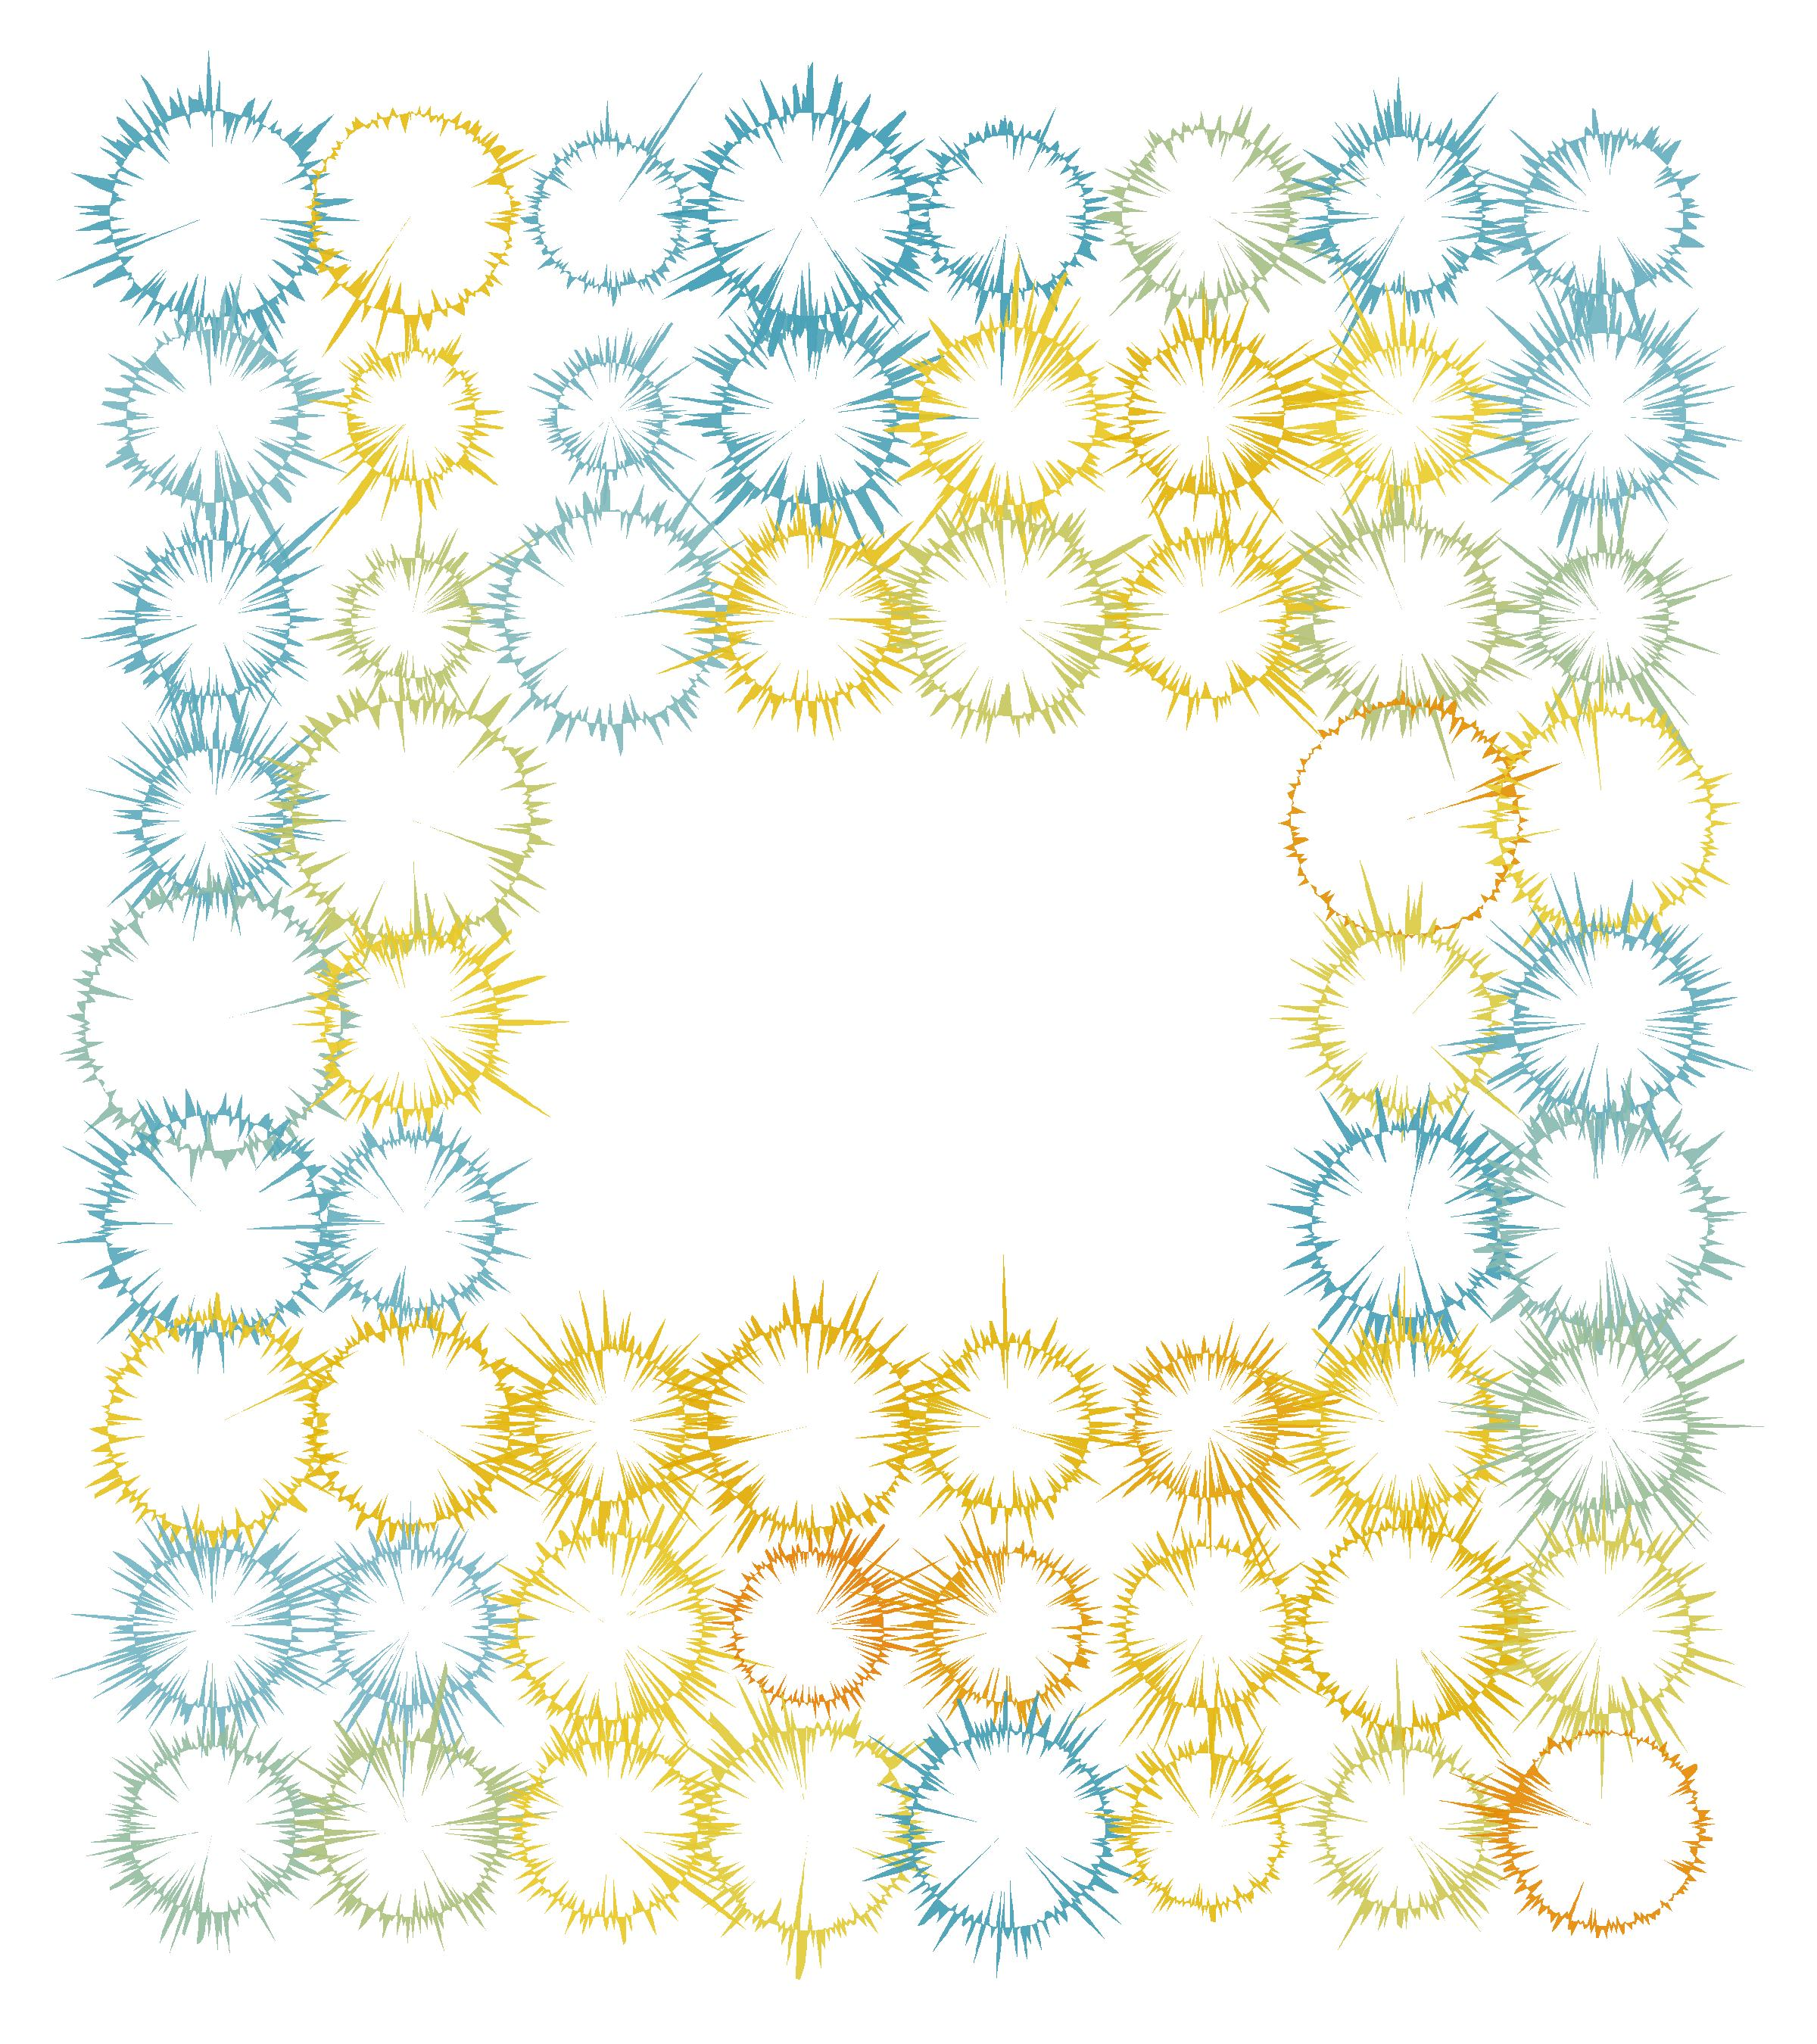
\includegraphics[width=2.60417in,height=\textheight]{cover.jpg}}

This website is the online version of \emph{Tidy Finance with R}, a book currently under development and intended for eventual print release. The book is the result of a joint effort of \href{https://christophscheuch.github.io/}{Christoph Scheuch}, \href{https://voigtstefan.me/}{Stefan Voigt}, and \href{https://sites.google.com/view/patrick-weiss}{Patrick Weiss}.

We are grateful for any kind of feedback on \emph{every} aspect of the book. So please get in touch with us via \href{mailto:contact@tidy-finance.org}{\nolinkurl{contact@tidy-finance.org}} if you spot typos, discover any issues that deserve more attention, or if you have suggestions for additional chapters and sections. Additionally, let us know if you found the text helpful. We look forward to hearing from you!

\hypertarget{why-does-this-book-exist}{%
\section*{Why does this book exist?}\label{why-does-this-book-exist}}


Financial economics is a vibrant area of research, a central part of all businesses activities, and at least implicitly relevant for our everyday life. Despite its relevance for our society and a vast number of empirical studies of financial phenomenons, one quickly learns that the actual implementation is typically rather opaque.
As graduate students, we were particularly surprised by the lack of public code for seminal papers or even textbooks on key concepts of financial economics. The lack of transparent code not only leads to numerous replication efforts (and their failures), but it also constitutes a waste of resources on problems that have already been solved by countless others in secrecy.

This book aims to lift the curtain on reproducible finance by providing a fully transparent code base for many common financial applications. We hope to inspire others to share their code publicly and take part in our journey towards more reproducible research in the future.

\hypertarget{who-should-read-this-book}{%
\section*{Who should read this book?}\label{who-should-read-this-book}}


We write this book for three audiences:

\begin{itemize}
\tightlist
\item
  Students who want to acquire the basic tools required to conduct financial research ranging from undergrad to graduate level. The book's structure is simple enough such that the material is sufficient for self-study purposes.
\item
  Instructors who look for materials to teach in empirical finance courses. We provide plenty of examples and (hopefully) intuitive explanations which can easily be adjusted or expanded.\\
\item
  Data analysts or statisticians who work on issues pertaining to financial data and need practical tools to do so.
\end{itemize}

Our book is close in spirit to \citet{Regenstein2018} and \citet{Coqueret2020} in that we provide fully reproducible code for useful applications and methods in finance.

The book ``Reproducible Finance with R'' provides an excellent introduction and discussion of different tools (based on the tidyverse, tidyquant, and xts) for standard applications in finance (e.g., how to compute returns and sample standard deviations of a time series of stock returns). Our book, in contrast, has a clear focus on applications of state-of-the-art for academic research in finance. We thus fill a niche that allows aspiring researchers or instructors to rely on a well-designed code base.

The book ``Machine Learning for Factor Investing'' is a great compendium to our book with respect to applications related to return prediction and portfolio formation. The book primarily targets practitioners and has a hands-on focus. Our book, in contrast, relies on the typical databases used in financial research and focuses on the preparation of such datasets for academic applications. In addition, our chapter on machine learning focuses on factor selection instead of return prediction.

\hypertarget{what-will-you-learn}{%
\section*{What will you learn?}\label{what-will-you-learn}}


The book is currently divided into 5 parts:

\begin{itemize}
\tightlist
\item
  Chapter 1 introduces you to important concepts around which our approach to Tidy Finance revolves.
\item
  Chapter 2 provides tools to organize your data and prepare the most common data sets used in financial research: CRSP and Compustat. We reuse the data from this chapter in all following chapters.
\item
  Chapters 3-7 deal with key concepts of empirical asset pricing such as beta estimation, portfolio sorts, and performance analysis.
\item
  Chapters 8-9 apply machine learning methods to problems in factor selection and option pricing.
\item
  Chapters 10-11 provide approaches for parametric, constrained portfolio optimization, and backtesting procedures.
\end{itemize}

Each chapter is self-contained and can be read individually. Yet the data chapter provides important background necessary for the data management in subsequent chapters. The number of chapters and covered content is subject to change as we will introduce additional material in the near future.

\hypertarget{what-wont-you-learn}{%
\section*{What won't you learn?}\label{what-wont-you-learn}}


This book is about empirical work. While we assume only basic knowledge in statistics and econometrics, we do not provide detailed treatments of the underlying theoretical models or methods applied in this book. Instead, you find references to the seminal academic work in journal articles and to more detailed treatments.
We believe that our comparative advantage is to provide a thorough implementation of portfolio sorts, backtesting procedures, machine learning methods, or other related topics in empirical finance and enrich these implementations with discussions of the needy-greedy choices you face while conducting empirical analyses. We hence refrain from deriving theoretical models or discussing the statistical properties of well-established tools.

\hypertarget{why-r}{%
\section*{Why R?}\label{why-r}}


We believe that R is among the best choices for a programming language in the area of finance. Some of our favorite features include:

\begin{itemize}
\tightlist
\item
  R is free and open-source so that you can use it in academic and professional contexts.
\item
  A diverse and active online community works on a broad range of tools.
\item
  A massive set of actively maintained packages for all kinds of applications exists, e.g., data manipulation, visualization, machine learning, etc.
\item
  Powerful tools for communication, e.g., Rmarkdown and shiny, are readily available.
\item
  RStudio is one of the best development environments for interactive data analysis.
\item
  Strong foundations of functional programming are provided.
\item
  Smooth integration with other programming languages, e.g., SQL, Python, C, C++, Fortran, etc.
\end{itemize}

For more information, we refer to \citet{Wickham2019}.

\hypertarget{why-tidy}{%
\section*{Why tidy?}\label{why-tidy}}


As you start working with data, you quickly realize that you spend a lot of time reading, cleaning, and transforming your data. In fact, it is often said that more than 80\% of data analysis is spent on preparing data. By \emph{tidying data}, we want to structure data sets to facilitate further analyses. As \citet{Wickham2014} puts it:

\begin{quote}
{[}T{]}idy datasets are all alike, but every messy dataset is messy in its own way. Tidy datasets provide a standardized way to link the structure of a dataset (its physical layout) with its semantics (its meaning).
\end{quote}

In its essence, tidy data follows these three principles:

\begin{enumerate}
\def\labelenumi{\arabic{enumi}.}
\tightlist
\item
  Every column is a variable.
\item
  Every row is an observation.
\item
  Every cell is a single value.
\end{enumerate}

Throughout this book, we try to follow these principles as best as we can. If you want to learn more about tidy data principles in an informal manner, we refer you to \href{https://cran.r-project.org/web/packages/tidyr/vignettes/tidy-data.html}{this vignette}.

In addition to the data layer, there are also tidy coding principles outlined in \href{https://tidyverse.tidyverse.org/articles/manifesto.html}{the tidy tools manifesto} that we try to follow:

\begin{enumerate}
\def\labelenumi{\arabic{enumi}.}
\tightlist
\item
  Reuse existing data structures.
\item
  Compose simple functions with the pipe.
\item
  Embrace functional programming.
\item
  Design for humans.
\end{enumerate}

In particular, we heavily draw on a set of packages called the \href{https://tidyverse.tidyverse.org/index.html}{\texttt{tidyverse}} \citep{Wickham2019}. The \texttt{tidyverse} is a consistent set of packages for all data analysis tasks, ranging from importing and wrangling to visualizing and modeling data with the same grammar. In addition to explicit tidy principles, the \texttt{tidyverse} has further benefits: (i) if you master one package, it is easier to master others, and (ii) the core packages are developed and maintained by the Public Benefit Company RStudio, Inc.~

Throughout the book we use the pipe \texttt{\textbar{}\textgreater{}}, a powerful tool to clearly express a sequence of operations. Readers familiar with the \texttt{tidyverse} may be used to the predecessor \texttt{\%\textgreater{}\%} by the \texttt{magrittr} package. For simple cases \texttt{\textbar{}\textgreater{}} and \texttt{\%\textgreater{}\%} behave identically, however, we follow Hadley Wickhams note ``the main advantage of \texttt{\textbar{}\textgreater{}} is that it does less than \texttt{\%\textgreater{}\%}, i.e.~it has what is important about the pipe with less of what is not important.'' For a more thorough discussion on the subtle differences, we refer to the \href{https://r4ds.hadley.nz/workflow-pipes.html}{second edition} of \citet{Wickham2016}.

\hypertarget{prerequisites}{%
\section*{Prerequisites}\label{prerequisites}}


Before we continue, make sure you have all the software you need for this book:

\begin{itemize}
\tightlist
\item
  \href{https://rstudio-education.github.io/hopr/starting.html\#starting}{Install R and RStudio}. To get a walk-through of the installation for every major operating system, follow the steps outlined \href{https://rstudio-education.github.io/hopr/starting.html\#starthng}{in this summary}. The whole process should be done in a few clicks. If you wonder about the difference: R is an open-source language and environment for statistical computing and graphics, free to download and use. While R runs the computations, RStudio is an integrated development environment that provides an interface by adding many convenient features and tools. We suggest doing all the coding in RStudio.
\item
  Open RStudio and \href{https://tidyverse.tidyverse.org/}{install the \texttt{tidyverse}}. Not sure how it works? You find helpful information on how to install packages in this \href{https://rstudio-education.github.io/hopr/packages2.html}{brief summary}.
\end{itemize}

If you are new to R, we recommend starting with the following sources:

\begin{itemize}
\tightlist
\item
  A very gentle and good introduction into the workings of R can be found in the form of the \href{https://rstudio-education.github.io/hopr/project-1-weighted-dice.html}{weighted dice project}. Once you are done setting up R on your machine, try to follow the instructions in this project.
\item
  The main book on the \texttt{tidyverse}, \citet{Wickham2016} is available online and for free: \href{https://r4ds.had.co.nz/introduction.html}{R for Data Science} by Hadley Wickham and Garrett Grolemund explains the majority of the tools we use in our book.
\item
  If you are an instructor searching for effectively teach R and data science methods, we recommend to take a look on the excellent \href{https://datasciencebox.org/}{data science toolbox} by \href{https://mine-cr.com/about/}{Mine Cetinkaya-Rundel}.
\item
  RStudio provides a range of excellent \href{https://www.rstudio.com/resources/cheatsheets/}{cheat sheets} with abundand information on how to use the \texttt{tidyverse} packages.
\end{itemize}

\hypertarget{about-the-authors}{%
\section*{About the authors}\label{about-the-authors}}


We met at the \href{https://www.vgsf.ac.at/}{Vienna Graduate School of Finance} from which each of us graduated with a different focus but a shared passion: coding with R. We continue to sharpen our R skills as part of our current occupations:

\begin{itemize}
\tightlist
\item
  \href{https://christophscheuch.github.io/}{Christoph Scheuch} is the Director of Product at the social trading platform \href{https://www.wikifolio.com/}{wikifolio.com} where he is responsible for product planning, execution, and monitoring. He also manages a team of data scientists to analyze user behavior and develop new products.
\item
  \href{https://voigtstefan.me/}{Stefan Voigt} is an Assistant Professor of Finance at the \href{https://www.economics.ku.dk/}{Department of Economics at the University in Copenhagen} and a research fellow at the \href{https://danishfinanceinstitute.dk/}{Danish Finance Institute}. His research focuses on blockchain technology, high-frequency trading, and financial econometrics. Stefan teaches parts of this book in his courses on empirical finance.
\item
  \href{https://sites.google.com/view/patrick-weiss}{Patrick Weiss} is a Post-Doc at the \href{https://www.wu.ac.at/en/}{Vienna University of Economics and Business}. His research centers around the intersection between asset pricing and corporate finance.
\end{itemize}

\hypertarget{license}{%
\section*{License}\label{license}}


This book is licensed to you under \href{https://creativecommons.org/licenses/by-nc-sa/4.0/}{Creative Commons Attribution-NonCommercial-ShareAlike 4.0 International CC BY-NC-SA 4.0}.

The code samples in this book are licensed under \href{https://creativecommons.org/publicdomain/zero/1.0/}{Creative Commons CC0 1.0 Universal (CC0 1.0), i.e., public domain}.

\hypertarget{colophon}{%
\section*{Colophon}\label{colophon}}


This book was written in RStudio using bookdown. The website is hosted with github pages and automatically updated after every commit. The complete source is \href{www.github.com/voigtstefan/tidy_finance}{available from GitHub}.
We generated all plots in this book using \texttt{ggplot2} and its classic dark-on-light theme (\texttt{theme\_bw()}).

This version of the book was built with R version 4.2.1 (2022-06-23, Funny-Looking Kid) and the following packages:

\begin{tabular}[t]{l|l}
\hline
Package & Version\\
\hline
alabama & 2022.4-1\\
\hline
bookdown & 0.27\\
\hline
broom & 1.0.0\\
\hline
dbplyr & 2.2.1\\
\hline
dplyr & 1.0.9\\
\hline
forcats & 0.5.1\\
\hline
frenchdata & 0.2.0\\
\hline
furrr & 0.3.0\\
\hline
ggplot2 & 3.3.6\\
\hline
glmnet & 4.1-4\\
\hline
googledrive & 2.0.0\\
\hline
hardhat & 1.2.0\\
\hline
jsonlite & 1.8.0\\
\hline
kableExtra & 1.3.4\\
\hline
keras & 2.9.0\\
\hline
knitr & 1.39\\
\hline
lmtest & 0.9-40\\
\hline
lubridate & 1.8.0\\
\hline
purrr & 0.3.4\\
\hline
quadprog & 1.5-8\\
\hline
ranger & 0.14.1\\
\hline
readr & 2.1.2\\
\hline
readxl & 1.4.0\\
\hline
renv & 0.15.5\\
\hline
rlang & 1.0.3\\
\hline
rmarkdown & 2.14\\
\hline
RPostgres & 1.4.4\\
\hline
RSQLite & 2.2.14\\
\hline
sandwich & 3.0-2\\
\hline
scales & 1.2.0\\
\hline
slider & 0.2.2\\
\hline
stringr & 1.4.0\\
\hline
tibble & 3.1.7\\
\hline
tidymodels & 0.2.0\\
\hline
tidyquant & 1.0.4\\
\hline
tidyr & 1.2.0\\
\hline
tidyverse & 1.3.1\\
\hline
timetk & 2.8.1\\
\hline
wesanderson & 0.3.6\\
\hline
\end{tabular}

\hypertarget{part-getting-started}{%
\part*{Getting started}\label{part-getting-started}}


\hypertarget{introduction-to-tidy-finance}{%
\chapter{Introduction to Tidy Finance}\label{introduction-to-tidy-finance}}

The main aim of this chapter is to familiarize yourself with the \texttt{tidyverse}. We start by downloading and visualizing stock data before moving to a simple portfolio choice problem. These examples introduce you to our approach of \emph{Tidy Finance}.

\hypertarget{working-with-stock-market-data}{%
\section{Working with stock market data}\label{working-with-stock-market-data}}

At the start of each session, we load the required packages.
Throughout the entire book, we always use the package \texttt{tidyverse}.
In this chapter, we also load the convenient \texttt{tidyquant} package to download price data.
You typically have to install a package once before you can load it. In case you have not done this yet, call \texttt{install.packages("tidyquant")}.
If you have trouble using \texttt{tidyquant}, check out the \href{https://cran.r-project.org/web/packages/tidyquant/vignettes/TQ01-core-functions-in-tidyquant.html\#yahoo-finance}{documentation}.

\begin{Shaded}
\begin{Highlighting}[]
\FunctionTok{library}\NormalTok{(tidyverse)}
\FunctionTok{library}\NormalTok{(tidyquant)}
\end{Highlighting}
\end{Shaded}

We first download daily prices for one stock market ticker, e.g., \emph{AAPL}, directly from the data provider Yahoo!Finance.
To download the data, you can use the command \texttt{tq\_get}. If you do not know how to use it, make sure you read the help file by calling \texttt{?tq\_get}.
We especially recommend taking a look at the documentation's examples section.

\begin{Shaded}
\begin{Highlighting}[]
\NormalTok{prices }\OtherTok{\textless{}{-}} \FunctionTok{tq\_get}\NormalTok{(}\StringTok{"AAPL"}\NormalTok{,}
  \AttributeTok{get =} \StringTok{"stock.prices"}\NormalTok{,}
  \AttributeTok{from =} \StringTok{"2000{-}01{-}01"}\NormalTok{,}
  \AttributeTok{to =} \StringTok{"2022{-}03{-}30"}
\NormalTok{)}
\NormalTok{prices}
\end{Highlighting}
\end{Shaded}

\begin{verbatim}
## # A tibble: 5,596 x 8
##   symbol date        open  high   low close    volume
##   <chr>  <date>     <dbl> <dbl> <dbl> <dbl>     <dbl>
## 1 AAPL   2000-01-03 0.936 1.00  0.908 0.999 535796800
## 2 AAPL   2000-01-04 0.967 0.988 0.903 0.915 512377600
## 3 AAPL   2000-01-05 0.926 0.987 0.920 0.929 778321600
## 4 AAPL   2000-01-06 0.948 0.955 0.848 0.848 767972800
## 5 AAPL   2000-01-07 0.862 0.902 0.853 0.888 460734400
## # ... with 5,591 more rows, and 1 more variable:
## #   adjusted <dbl>
\end{verbatim}

\texttt{tq\_get} downloads stock market data from Yahoo!Finance if you do not specify another data source. The function returns a tibble with eight quite self-explanatory columns: \emph{symbol}, \emph{date}, the market prices at the \emph{open, high, low} and \emph{close}, the daily \emph{volume} (in number of traded shares), and the \emph{adjusted} price in USD. The adjusted prices are corrected for anything that might affect the stock price after the market closes, e.g., stock splits and dividends. These actions affect the quoted prices, but they have no direct impact on the investors who hold the stock.

Next, we use \texttt{ggplot2} to visualize the time series of adjusted prices.

\begin{Shaded}
\begin{Highlighting}[]
\NormalTok{prices }\SpecialCharTok{|}\ErrorTok{\textgreater{}}
  \FunctionTok{ggplot}\NormalTok{(}\FunctionTok{aes}\NormalTok{(}\AttributeTok{x =}\NormalTok{ date, }\AttributeTok{y =}\NormalTok{ adjusted)) }\SpecialCharTok{+}
  \FunctionTok{geom\_line}\NormalTok{() }\SpecialCharTok{+}
  \FunctionTok{labs}\NormalTok{(}
    \AttributeTok{x =} \ConstantTok{NULL}\NormalTok{,}
    \AttributeTok{y =} \ConstantTok{NULL}\NormalTok{,}
    \AttributeTok{title =} \StringTok{"AAPL stock prices"}\NormalTok{,}
    \AttributeTok{subtitle =} \StringTok{"Prices in USD, adjusted for dividend payments and stock splits"}
\NormalTok{  )}
\end{Highlighting}
\end{Shaded}

\begin{center}\includegraphics{10_introduction_files/figure-latex/unnamed-chunk-3-1} \end{center}

Instead of analyzing prices, we compute daily returns defined as \((p_t - p_{t-1}) / p_{t-1}\) where \(p_t\) is the adjusted day \(t\) price. The function \texttt{lag} computes the previous value in a vector.

\begin{Shaded}
\begin{Highlighting}[]
\NormalTok{returns }\OtherTok{\textless{}{-}}\NormalTok{ prices }\SpecialCharTok{|}\ErrorTok{\textgreater{}}
  \FunctionTok{arrange}\NormalTok{(date) }\SpecialCharTok{|}\ErrorTok{\textgreater{}}
  \FunctionTok{mutate}\NormalTok{(}\AttributeTok{ret =}\NormalTok{ (adjusted }\SpecialCharTok{{-}} \FunctionTok{lag}\NormalTok{(adjusted)) }\SpecialCharTok{/} \FunctionTok{lag}\NormalTok{(adjusted)) }\SpecialCharTok{|}\ErrorTok{\textgreater{}}
  \FunctionTok{select}\NormalTok{(symbol, date, ret)}
\NormalTok{returns}
\end{Highlighting}
\end{Shaded}

\begin{verbatim}
## # A tibble: 5,596 x 3
##   symbol date           ret
##   <chr>  <date>       <dbl>
## 1 AAPL   2000-01-03 NA     
## 2 AAPL   2000-01-04 -0.0843
## 3 AAPL   2000-01-05  0.0146
## 4 AAPL   2000-01-06 -0.0865
## 5 AAPL   2000-01-07  0.0474
## # ... with 5,591 more rows
\end{verbatim}

The resulting tibble contains three columns where the last contains the daily returns. Note that the first entry naturally contains \texttt{NA} because there is no previous price. Additionally, the computations require that the time series is ordered by date.
Otherwise, \texttt{lag} would be meaningless.

For the upcoming examples, we remove missing values as these would require separate treatment when computing, e.g., sample averages. In general, however, make sure you understand why \texttt{NA} values occur and carefully examine if you can simply get rid of these observations.

\begin{Shaded}
\begin{Highlighting}[]
\NormalTok{returns }\OtherTok{\textless{}{-}}\NormalTok{ returns }\SpecialCharTok{|}\ErrorTok{\textgreater{}}
  \FunctionTok{drop\_na}\NormalTok{(ret)}
\end{Highlighting}
\end{Shaded}

Next, we visualize the distribution of daily returns in a histogram. For convenience, we multiply the returns by 100 to get returns in percent for the visualizations. Additionally, we also add a dashed red line that indicates the 5\% quantile of the daily returns to the histogram, which is a (crude) proxy for the worst return of the stock with a probability of at least 5\%.

\begin{Shaded}
\begin{Highlighting}[]
\NormalTok{quantile\_05 }\OtherTok{\textless{}{-}} \FunctionTok{quantile}\NormalTok{(returns }\SpecialCharTok{|}\ErrorTok{\textgreater{}} \FunctionTok{pull}\NormalTok{(ret) }\SpecialCharTok{*} \DecValTok{100}\NormalTok{, }\FloatTok{0.05}\NormalTok{)}

\NormalTok{returns }\SpecialCharTok{|}\ErrorTok{\textgreater{}}
  \FunctionTok{ggplot}\NormalTok{(}\FunctionTok{aes}\NormalTok{(}\AttributeTok{x =}\NormalTok{ ret }\SpecialCharTok{*} \DecValTok{100}\NormalTok{)) }\SpecialCharTok{+}
  \FunctionTok{geom\_histogram}\NormalTok{(}\AttributeTok{bins =} \DecValTok{100}\NormalTok{) }\SpecialCharTok{+}
  \FunctionTok{geom\_vline}\NormalTok{(}\FunctionTok{aes}\NormalTok{(}\AttributeTok{xintercept =}\NormalTok{ quantile\_05),}
    \AttributeTok{color =} \StringTok{"red"}\NormalTok{,}
    \AttributeTok{linetype =} \StringTok{"dashed"}
\NormalTok{  ) }\SpecialCharTok{+}
  \FunctionTok{labs}\NormalTok{(}
    \AttributeTok{x =} \ConstantTok{NULL}\NormalTok{,}
    \AttributeTok{y =} \ConstantTok{NULL}\NormalTok{,}
    \AttributeTok{title =} \StringTok{"Distribution of daily AAPL returns (in percent)"}\NormalTok{,}
    \AttributeTok{subtitle =} \StringTok{"The dotted vertical line indicates the historical 5\% quantile"}
\NormalTok{  )}
\end{Highlighting}
\end{Shaded}

\begin{center}\includegraphics{10_introduction_files/figure-latex/unnamed-chunk-6-1} \end{center}

Here, \texttt{bins\ =\ 100} determines the number of bins and hence implicitly the width of the bins.
Before proceeding, make sure you understand how to use the geom \texttt{geom\_vline()} to add a dotted red line that indicates the 5\% quantile of the daily returns.
A typical task before proceeding with \emph{any} data is to compute summary statistics for the main variables of interest.

\begin{Shaded}
\begin{Highlighting}[]
\NormalTok{returns }\SpecialCharTok{|}\ErrorTok{\textgreater{}}
  \FunctionTok{mutate}\NormalTok{(}\AttributeTok{ret =}\NormalTok{ ret }\SpecialCharTok{*} \DecValTok{100}\NormalTok{) }\SpecialCharTok{|}\ErrorTok{\textgreater{}}
  \FunctionTok{summarize}\NormalTok{(}\FunctionTok{across}\NormalTok{(}
\NormalTok{    ret,}
    \FunctionTok{list}\NormalTok{(}
      \AttributeTok{daily\_mean =}\NormalTok{ mean,}
      \AttributeTok{daily\_sd =}\NormalTok{ sd,}
      \AttributeTok{daily\_min =}\NormalTok{ min,}
      \AttributeTok{daily\_max =}\NormalTok{ max}
\NormalTok{    )}
\NormalTok{  ))}
\end{Highlighting}
\end{Shaded}

\begin{verbatim}
## # A tibble: 1 x 4
##   ret_daily_mean ret_daily_sd ret_daily_min
##            <dbl>        <dbl>         <dbl>
## 1          0.129         2.52         -51.9
## # ... with 1 more variable: ret_daily_max <dbl>
\end{verbatim}

We see that the maximum \emph{daily} return was around 13.905 percent.\\
You can also compute these summary statistics for each year by imposing \texttt{group\_by(year\ =\ year(date))}, where the call \texttt{year(date)} computes the year.

\begin{Shaded}
\begin{Highlighting}[]
\NormalTok{returns }\SpecialCharTok{|}\ErrorTok{\textgreater{}}
  \FunctionTok{mutate}\NormalTok{(}\AttributeTok{ret =}\NormalTok{ ret }\SpecialCharTok{*} \DecValTok{100}\NormalTok{) }\SpecialCharTok{|}\ErrorTok{\textgreater{}}
  \FunctionTok{group\_by}\NormalTok{(}\AttributeTok{year =} \FunctionTok{year}\NormalTok{(date)) }\SpecialCharTok{|}\ErrorTok{\textgreater{}}
  \FunctionTok{summarize}\NormalTok{(}\FunctionTok{across}\NormalTok{(}
\NormalTok{    ret,}
    \FunctionTok{list}\NormalTok{(}
      \AttributeTok{daily\_mean =}\NormalTok{ mean,}
      \AttributeTok{daily\_sd =}\NormalTok{ sd,}
      \AttributeTok{daily\_min =}\NormalTok{ min,}
      \AttributeTok{daily\_max =}\NormalTok{ max}
\NormalTok{    ),}
    \AttributeTok{.names =} \StringTok{"\{.fn\}"}
\NormalTok{  ))}
\end{Highlighting}
\end{Shaded}

\begin{verbatim}
## # A tibble: 23 x 5
##    year daily_mean daily_sd daily_min daily_max
##   <dbl>      <dbl>    <dbl>     <dbl>     <dbl>
## 1  2000     -0.346     5.49    -51.9      13.7 
## 2  2001      0.233     3.93    -17.2      12.9 
## 3  2002     -0.121     3.05    -15.0       8.46
## 4  2003      0.186     2.34     -8.14     11.3 
## 5  2004      0.470     2.55     -5.58     13.2 
## # ... with 18 more rows
\end{verbatim}

In case you wonder: the additional argument \texttt{.names\ =\ "\{.fn\}"} in \texttt{across()} determines how to name the output columns. The specification is rather flexible and allows almost arbitrary column names, which can be useful for reporting.

\hypertarget{scaling-up-the-analysis}{%
\section{Scaling up the analysis}\label{scaling-up-the-analysis}}

As a next step, we generalize the code from before such that all the computations can handle an arbitrary vector of tickers (e.g., all constituents of an index). Following tidy principles, it is quite easy to download the data, plot the price time series, and tabulate the summary statistics for an arbitrary number of assets.

This is where the \texttt{tidyverse} magic starts: tidy data makes it extremely easy to generalize the computations from before to as many assets you like. The following code takes any vector of tickers, e.g., \texttt{ticker\ \textless{}-\ c("AAPL",\ "MMM",\ "BA")}, and automates the download as well as the plot of the price time series. In the end, we create the table of summary statistics for an arbitrary number of assets. We perform the analysis with data from all current constituents of the \href{https://en.wikipedia.org/wiki/Dow_Jones_Industrial_Average}{Dow Jones Industrial Average index}.

\begin{Shaded}
\begin{Highlighting}[]
\NormalTok{ticker }\OtherTok{\textless{}{-}} \FunctionTok{tq\_index}\NormalTok{(}\StringTok{"DOW"}\NormalTok{)}
\NormalTok{index\_prices }\OtherTok{\textless{}{-}} \FunctionTok{tq\_get}\NormalTok{(ticker,}
  \AttributeTok{get =} \StringTok{"stock.prices"}\NormalTok{,}
  \AttributeTok{from =} \StringTok{"2000{-}01{-}01"}\NormalTok{,}
  \AttributeTok{to =} \StringTok{"2022{-}03{-}30"}
\NormalTok{)}
\end{Highlighting}
\end{Shaded}

The resulting file contains 159863 daily observations for in total 30 different corporations. The figure below illustrates the time series of downloaded \emph{adjusted} prices for each of the constituents of the Dow Jones index. Make sure you understand every single line of code! (What are the arguments of \texttt{aes()}? Which alternative geoms could you use to visualize the time series? Hint: if you do not know the answers try to change the code to see what difference your intervention causes).

\begin{Shaded}
\begin{Highlighting}[]
\NormalTok{index\_prices }\SpecialCharTok{|}\ErrorTok{\textgreater{}}
  \FunctionTok{ggplot}\NormalTok{(}\FunctionTok{aes}\NormalTok{(}
    \AttributeTok{x =}\NormalTok{ date,}
    \AttributeTok{y =}\NormalTok{ adjusted,}
    \AttributeTok{color =}\NormalTok{ symbol}
\NormalTok{  )) }\SpecialCharTok{+}
  \FunctionTok{geom\_line}\NormalTok{() }\SpecialCharTok{+}
  \FunctionTok{labs}\NormalTok{(}
    \AttributeTok{x =} \ConstantTok{NULL}\NormalTok{,}
    \AttributeTok{y =} \ConstantTok{NULL}\NormalTok{,}
    \AttributeTok{color =} \ConstantTok{NULL}\NormalTok{,}
    \AttributeTok{title =} \StringTok{"DOW index stock prices"}\NormalTok{,}
    \AttributeTok{subtitle =} \StringTok{"Prices in USD, adjusted for dividend payments and stock splits"}
\NormalTok{  ) }\SpecialCharTok{+}
  \FunctionTok{theme}\NormalTok{(}\AttributeTok{legend.position =} \StringTok{"none"}\NormalTok{)}
\end{Highlighting}
\end{Shaded}

\begin{center}\includegraphics{10_introduction_files/figure-latex/unnamed-chunk-9-1} \end{center}

Do you notice the small differences relative to the code we used before? \texttt{tq\_get(ticker)} returns a tibble for several symbols as well. All we need to do to illustrate all tickers simultaneously is to include \texttt{color\ =\ symbol} in the \texttt{ggplot2} aesthetics. In this way, we generate a separate line for each ticker. Of course, there are simply too many lines on this graph to properly identify the individual stocks, but it illustrates the point well.

The same holds for stock returns. Before computing the returns, we use \texttt{group\_by(symbol)} such that the \texttt{mutate} command is performed for each symbol individually. The same logic applies to the computation of summary statistics: \texttt{group\_by(symbol)} is the key to aggregating the time series into ticker-specific variables of interest.

\begin{Shaded}
\begin{Highlighting}[]
\NormalTok{all\_returns }\OtherTok{\textless{}{-}}\NormalTok{ index\_prices }\SpecialCharTok{|}\ErrorTok{\textgreater{}}
  \FunctionTok{group\_by}\NormalTok{(symbol) }\SpecialCharTok{|}\ErrorTok{\textgreater{}}
  \FunctionTok{mutate}\NormalTok{(}\AttributeTok{ret =}\NormalTok{ adjusted }\SpecialCharTok{/} \FunctionTok{lag}\NormalTok{(adjusted) }\SpecialCharTok{{-}} \DecValTok{1}\NormalTok{) }\SpecialCharTok{|}\ErrorTok{\textgreater{}}
  \FunctionTok{select}\NormalTok{(symbol, date, ret) }\SpecialCharTok{|}\ErrorTok{\textgreater{}}
  \FunctionTok{drop\_na}\NormalTok{(ret)}

\NormalTok{all\_returns }\SpecialCharTok{|}\ErrorTok{\textgreater{}}
  \FunctionTok{mutate}\NormalTok{(}\AttributeTok{ret =}\NormalTok{ ret }\SpecialCharTok{*} \DecValTok{100}\NormalTok{) }\SpecialCharTok{|}\ErrorTok{\textgreater{}}
  \FunctionTok{group\_by}\NormalTok{(symbol) }\SpecialCharTok{|}\ErrorTok{\textgreater{}}
  \FunctionTok{summarize}\NormalTok{(}\FunctionTok{across}\NormalTok{(}
\NormalTok{    ret,}
    \FunctionTok{list}\NormalTok{(}
      \AttributeTok{daily\_mean =}\NormalTok{ mean,}
      \AttributeTok{daily\_sd =}\NormalTok{ sd,}
      \AttributeTok{daily\_min =}\NormalTok{ min,}
      \AttributeTok{daily\_max =}\NormalTok{ max}
\NormalTok{    ),}
    \AttributeTok{.names =} \StringTok{"\{.fn\}"}
\NormalTok{  ))}
\end{Highlighting}
\end{Shaded}

\begin{verbatim}
## # A tibble: 30 x 5
##   symbol daily_mean daily_sd daily_min daily_max
##   <chr>       <dbl>    <dbl>     <dbl>     <dbl>
## 1 AAPL       0.129      2.52     -51.9      13.9
## 2 AMGN       0.0484     1.98     -13.4      15.1
## 3 AXP        0.0572     2.30     -17.6      21.9
## 4 BA         0.0603     2.20     -23.8      24.3
## 5 CAT        0.0707     2.03     -14.5      14.7
## # ... with 25 more rows
\end{verbatim}

Note that you are now also equipped with all tools to download price data for \emph{each} ticker listed in the S\&P 500 index with the same number of lines of code. Just use \texttt{ticker\ \textless{}-\ tq\_index("SP500")}, which provides you with a tibble that contains each symbol that is (currently) part of the S\&P 500. However, don't try this if you are not prepared to wait for a couple of minutes because this is quite some data to download!

\hypertarget{other-forms-of-data-aggregation}{%
\section{Other forms of data aggregation}\label{other-forms-of-data-aggregation}}

Of course, aggregation across other variables than \texttt{symbol} can make sense as well. For instance, suppose you are interested in answering the question: are days with high aggregate trading volume likely followed by days with high aggregate trading volume? To provide some initial analysis on this question, we take the downloaded prices and compute aggregate daily trading volume for all Dow Jones constituents in USD. Recall that the column \emph{volume} is denoted in the number of traded shares. Thus, we multiply the trading volume with the daily closing price to get a proxy for the aggregate trading volume in USD. Scaling by \texttt{1e9} denotes daily trading volume in billion USD.

\begin{Shaded}
\begin{Highlighting}[]
\NormalTok{volume }\OtherTok{\textless{}{-}}\NormalTok{ index\_prices }\SpecialCharTok{|}\ErrorTok{\textgreater{}}
  \FunctionTok{mutate}\NormalTok{(}\AttributeTok{volume\_usd =}\NormalTok{ volume }\SpecialCharTok{*}\NormalTok{ close }\SpecialCharTok{/} \FloatTok{1e9}\NormalTok{) }\SpecialCharTok{|}\ErrorTok{\textgreater{}}
  \FunctionTok{group\_by}\NormalTok{(date) }\SpecialCharTok{|}\ErrorTok{\textgreater{}}
  \FunctionTok{summarize}\NormalTok{(}\AttributeTok{volume =} \FunctionTok{sum}\NormalTok{(volume\_usd))}

\NormalTok{volume }\SpecialCharTok{|}\ErrorTok{\textgreater{}}
  \FunctionTok{ggplot}\NormalTok{(}\FunctionTok{aes}\NormalTok{(}\AttributeTok{x =}\NormalTok{ date, }\AttributeTok{y =}\NormalTok{ volume)) }\SpecialCharTok{+}
  \FunctionTok{geom\_line}\NormalTok{() }\SpecialCharTok{+}
  \FunctionTok{labs}\NormalTok{(}
    \AttributeTok{x =} \ConstantTok{NULL}\NormalTok{, }\AttributeTok{y =} \ConstantTok{NULL}\NormalTok{,}
    \AttributeTok{title =} \StringTok{"Aggregate daily trading volume (billion USD)"}
\NormalTok{  )}
\end{Highlighting}
\end{Shaded}

\begin{center}\includegraphics{10_introduction_files/figure-latex/unnamed-chunk-11-1} \end{center}

One way to illustrate the persistence of trading volume would be to plot volume on day \(t\) against volume on day \(t-1\) as in the example below. We add a 45°-line to indicate a hypothetical one-to-one relation by \texttt{geom\_abline}, addressing potential differences in the axes' scales.

\begin{Shaded}
\begin{Highlighting}[]
\NormalTok{volume }\SpecialCharTok{|}\ErrorTok{\textgreater{}}
  \FunctionTok{ggplot}\NormalTok{(}\FunctionTok{aes}\NormalTok{(}\AttributeTok{x =} \FunctionTok{lag}\NormalTok{(volume), }\AttributeTok{y =}\NormalTok{ volume)) }\SpecialCharTok{+}
  \FunctionTok{geom\_point}\NormalTok{() }\SpecialCharTok{+}
  \FunctionTok{geom\_abline}\NormalTok{(}\FunctionTok{aes}\NormalTok{(}\AttributeTok{intercept =} \DecValTok{0}\NormalTok{, }\AttributeTok{slope =} \DecValTok{1}\NormalTok{),}
    \AttributeTok{color =} \StringTok{"red"}\NormalTok{,}
    \AttributeTok{linetype =} \StringTok{"dotted"}
\NormalTok{  ) }\SpecialCharTok{+}
  \FunctionTok{labs}\NormalTok{(}
    \AttributeTok{x =} \StringTok{"Previous day aggregate trading volume (billion USD)"}\NormalTok{,}
    \AttributeTok{y =} \StringTok{"Aggregate trading volume (billion USD)"}\NormalTok{,}
    \AttributeTok{title =} \StringTok{"Persistence of trading volume"}
\NormalTok{  )}
\end{Highlighting}
\end{Shaded}

\begin{verbatim}
## Warning: Removed 1 rows containing missing values
## (geom_point).
\end{verbatim}

\begin{center}\includegraphics{10_introduction_files/figure-latex/unnamed-chunk-12-1} \end{center}

Do you understand where the warning \texttt{\#\#\ Warning:\ Removed\ 1\ rows\ containing\ missing\ values\ (geom\_point).} comes from and what it means? Purely eye-balling reveals that days with high trading volume are often followed by similarly high trading volume days.

\hypertarget{portfolio-choice-problems}{%
\section{Portfolio choice problems}\label{portfolio-choice-problems}}

In the previous part, we show how to download stock market data and inspect it with graphs and summary statistics. Now, we move to a typical question in Finance, namely, how to optimally allocate wealth across different assets. The standard framework for optimal portfolio selection considers investors that prefer higher future returns but dislike future return volatility (defined as the square root of the return variance): the \emph{mean-variance investor}.

An essential tool to evaluate portfolios in the mean-variance context is the \emph{efficient frontier}, the set of portfolios which satisfy the condition that no other portfolio exists with a higher expected return but with the same volatility (i.e., the risk). We compute and visualize the efficient frontier for several stocks.
First, we extract each asset's \emph{monthly} returns. In order to keep things simple, we work with a balanced panel and exclude tickers for which we do not observe a price on every single trading day since 2000.

\begin{Shaded}
\begin{Highlighting}[]
\NormalTok{index\_prices }\OtherTok{\textless{}{-}}\NormalTok{ index\_prices }\SpecialCharTok{|}\ErrorTok{\textgreater{}}
  \FunctionTok{group\_by}\NormalTok{(symbol) }\SpecialCharTok{|}\ErrorTok{\textgreater{}}
  \FunctionTok{mutate}\NormalTok{(}\AttributeTok{n =} \FunctionTok{n}\NormalTok{()) }\SpecialCharTok{|}\ErrorTok{\textgreater{}}
  \FunctionTok{ungroup}\NormalTok{() }\SpecialCharTok{|}\ErrorTok{\textgreater{}}
  \FunctionTok{filter}\NormalTok{(n }\SpecialCharTok{==} \FunctionTok{max}\NormalTok{(n)) }\SpecialCharTok{|}\ErrorTok{\textgreater{}}
  \FunctionTok{select}\NormalTok{(}\SpecialCharTok{{-}}\NormalTok{n)}

\NormalTok{returns }\OtherTok{\textless{}{-}}\NormalTok{ index\_prices }\SpecialCharTok{|}\ErrorTok{\textgreater{}}
  \FunctionTok{mutate}\NormalTok{(}\AttributeTok{month =} \FunctionTok{floor\_date}\NormalTok{(date, }\StringTok{"month"}\NormalTok{)) }\SpecialCharTok{|}\ErrorTok{\textgreater{}}
  \FunctionTok{group\_by}\NormalTok{(symbol, month) }\SpecialCharTok{|}\ErrorTok{\textgreater{}}
  \FunctionTok{summarize}\NormalTok{(}\AttributeTok{price =} \FunctionTok{last}\NormalTok{(adjusted), }\AttributeTok{.groups =} \StringTok{"drop\_last"}\NormalTok{) }\SpecialCharTok{|}\ErrorTok{\textgreater{}}
  \FunctionTok{mutate}\NormalTok{(}\AttributeTok{ret =}\NormalTok{ price }\SpecialCharTok{/} \FunctionTok{lag}\NormalTok{(price) }\SpecialCharTok{{-}} \DecValTok{1}\NormalTok{) }\SpecialCharTok{|}\ErrorTok{\textgreater{}}
  \FunctionTok{drop\_na}\NormalTok{(ret) }\SpecialCharTok{|}\ErrorTok{\textgreater{}}
  \FunctionTok{select}\NormalTok{(}\SpecialCharTok{{-}}\NormalTok{price)}
\end{Highlighting}
\end{Shaded}

Next, we transform the returns from a tidy tibble into a \((T \times N)\) matrix with one column for each of the \(N\) tickers to compute the covariance matrix \(\Sigma\) and also the expected return vector \(\mu\). We achieve this by using \texttt{pivot\_wider()} with the new column names from the column \texttt{symbol} and setting the values to \texttt{ret}.
We compute the vector of sample average returns and the sample variance-covariance matrix, which we consider as proxies for the parameters of future returns.

\begin{Shaded}
\begin{Highlighting}[]
\NormalTok{returns\_matrix }\OtherTok{\textless{}{-}}\NormalTok{ returns }\SpecialCharTok{|}\ErrorTok{\textgreater{}}
  \FunctionTok{pivot\_wider}\NormalTok{(}
    \AttributeTok{names\_from =}\NormalTok{ symbol,}
    \AttributeTok{values\_from =}\NormalTok{ ret}
\NormalTok{  ) }\SpecialCharTok{|}\ErrorTok{\textgreater{}}
  \FunctionTok{select}\NormalTok{(}\SpecialCharTok{{-}}\NormalTok{month)}

\NormalTok{sigma }\OtherTok{\textless{}{-}} \FunctionTok{cov}\NormalTok{(returns\_matrix)}
\NormalTok{mu }\OtherTok{\textless{}{-}} \FunctionTok{colMeans}\NormalTok{(returns\_matrix)}
\end{Highlighting}
\end{Shaded}

Then, we compute the minimum variance portfolio weights \(\omega_\text{mvp}\) as well as the expected return \(\omega_\text{mvp}'\mu\) and volatility \(\sqrt{\omega_\text{mvp}'\Sigma\omega_\text{mvp}}\) of this portfolio. Recall that the minimum variance portfolio is the vector of portfolio weights that are the solution to
\[\omega_\text{mvp} = \arg\min w'\Sigma w \text{ s.t. } \sum\limits_{i=1}^Nw_i = 1.\]
It is easy to show analytically, that \(\omega_\text{mvp} = \frac{\Sigma^{-1}\iota}{\iota'\Sigma^{-1}\iota}\) where \(\iota\) is a vector of ones.

\begin{Shaded}
\begin{Highlighting}[]
\NormalTok{N }\OtherTok{\textless{}{-}} \FunctionTok{ncol}\NormalTok{(returns\_matrix)}
\NormalTok{iota }\OtherTok{\textless{}{-}} \FunctionTok{rep}\NormalTok{(}\DecValTok{1}\NormalTok{, N)}
\NormalTok{mvp\_weights }\OtherTok{\textless{}{-}} \FunctionTok{solve}\NormalTok{(sigma) }\SpecialCharTok{\%*\%}\NormalTok{ iota}
\NormalTok{mvp\_weights }\OtherTok{\textless{}{-}}\NormalTok{ mvp\_weights }\SpecialCharTok{/} \FunctionTok{sum}\NormalTok{(mvp\_weights)}

\FunctionTok{tibble}\NormalTok{(}
  \AttributeTok{expected\_ret =} \FunctionTok{t}\NormalTok{(mvp\_weights) }\SpecialCharTok{\%*\%}\NormalTok{ mu,}
  \AttributeTok{volatility =} \FunctionTok{sqrt}\NormalTok{(}\FunctionTok{t}\NormalTok{(mvp\_weights) }\SpecialCharTok{\%*\%}\NormalTok{ sigma }\SpecialCharTok{\%*\%}\NormalTok{ mvp\_weights)}
\NormalTok{)}
\end{Highlighting}
\end{Shaded}

\begin{verbatim}
## # A tibble: 1 x 2
##   expected_ret[,1] volatility[,1]
##              <dbl>          <dbl>
## 1          0.00838         0.0314
\end{verbatim}

Note that the \emph{monthly} volatility of the minimum variance portfolio is of the same order of magnitude as the \emph{daily} standard deviation of the individual components. Thus, the diversification benefits in terms of risk reduction are tremendous!

Next, we set out to find the weights for a portfolio that achieves three times the expected return of the minimum variance portfolio. However, mean-variance investors are not interested in any portfolio that achieves the required return but rather in the efficient portfolio, i.e., the portfolio with the lowest standard deviation.
If you wonder where the solution \(\omega_\text{eff}\) comes from: The efficient portfolio is chosen by an investor who aims to achieve minimum variance \emph{given a minimum acceptable expected return} \(\bar{\mu}\). Hence, their objective function is to choose \(\omega_\text{eff}\) as the solution to
\[\omega_\text{eff}(\bar{\mu}) = \arg\min w'\Sigma w \text{ s.t. } w'\iota = 1 \text{ and } \omega'\mu \geq \bar{\mu}.\]
The code below implements the analytic solution to this optimization problem for a benchmark return \(\bar\mu\) which we set to 3 times the expected return of the minimum variance portfolio. We encourage you to verify that it is correct.

\begin{Shaded}
\begin{Highlighting}[]
\NormalTok{mu\_bar }\OtherTok{\textless{}{-}} \DecValTok{3} \SpecialCharTok{*} \FunctionTok{t}\NormalTok{(mvp\_weights) }\SpecialCharTok{\%*\%}\NormalTok{ mu}

\NormalTok{C }\OtherTok{\textless{}{-}} \FunctionTok{as.numeric}\NormalTok{(}\FunctionTok{t}\NormalTok{(iota) }\SpecialCharTok{\%*\%} \FunctionTok{solve}\NormalTok{(sigma) }\SpecialCharTok{\%*\%}\NormalTok{ iota)}
\NormalTok{D }\OtherTok{\textless{}{-}} \FunctionTok{as.numeric}\NormalTok{(}\FunctionTok{t}\NormalTok{(iota) }\SpecialCharTok{\%*\%} \FunctionTok{solve}\NormalTok{(sigma) }\SpecialCharTok{\%*\%}\NormalTok{ mu)}
\NormalTok{E }\OtherTok{\textless{}{-}} \FunctionTok{as.numeric}\NormalTok{(}\FunctionTok{t}\NormalTok{(mu) }\SpecialCharTok{\%*\%} \FunctionTok{solve}\NormalTok{(sigma) }\SpecialCharTok{\%*\%}\NormalTok{ mu)}

\NormalTok{lambda\_tilde }\OtherTok{\textless{}{-}} \FunctionTok{as.numeric}\NormalTok{(}\DecValTok{2} \SpecialCharTok{*}\NormalTok{ (mu\_bar }\SpecialCharTok{{-}}\NormalTok{ D }\SpecialCharTok{/}\NormalTok{ C) }\SpecialCharTok{/}\NormalTok{ (E }\SpecialCharTok{{-}}\NormalTok{ D}\SpecialCharTok{\^{}}\DecValTok{2} \SpecialCharTok{/}\NormalTok{ C))}
\NormalTok{efp\_weights }\OtherTok{\textless{}{-}}\NormalTok{ mvp\_weights }\SpecialCharTok{+}\NormalTok{ lambda\_tilde }\SpecialCharTok{/} \DecValTok{2} \SpecialCharTok{*}\NormalTok{ (}\FunctionTok{solve}\NormalTok{(sigma) }\SpecialCharTok{\%*\%}\NormalTok{ mu }\SpecialCharTok{{-}}\NormalTok{ D }\SpecialCharTok{/}\NormalTok{ C }\SpecialCharTok{*} \FunctionTok{solve}\NormalTok{(sigma) }\SpecialCharTok{\%*\%}\NormalTok{ iota)}
\end{Highlighting}
\end{Shaded}

\hypertarget{the-efficient-frontier}{%
\section{The efficient frontier}\label{the-efficient-frontier}}

The two mutual fund separation theorem states that as soon as we have two efficient portfolios (such as the minimum variance portfolio and the efficient portfolio for another required level of expected returns like above), we can characterize the entire efficient frontier by combining these two portfolios. The code below implements the construction of the \emph{efficient frontier}, which characterizes the highest expected return achievable at each level of risk. To understand the code better, make sure to familiarize yourself with the inner workings of the \texttt{for} loop.

\begin{Shaded}
\begin{Highlighting}[]
\NormalTok{c }\OtherTok{\textless{}{-}} \FunctionTok{seq}\NormalTok{(}\AttributeTok{from =} \SpecialCharTok{{-}}\FloatTok{0.4}\NormalTok{, }\AttributeTok{to =} \FloatTok{1.9}\NormalTok{, }\AttributeTok{by =} \FloatTok{0.01}\NormalTok{)}
\NormalTok{res }\OtherTok{\textless{}{-}} \FunctionTok{tibble}\NormalTok{(}
  \AttributeTok{c =}\NormalTok{ c,}
  \AttributeTok{mu =} \ConstantTok{NA}\NormalTok{,}
  \AttributeTok{sd =} \ConstantTok{NA}
\NormalTok{)}

\ControlFlowTok{for}\NormalTok{ (i }\ControlFlowTok{in} \FunctionTok{seq\_along}\NormalTok{(c)) \{}
\NormalTok{  w }\OtherTok{\textless{}{-}}\NormalTok{ (}\DecValTok{1} \SpecialCharTok{{-}}\NormalTok{ c[i]) }\SpecialCharTok{*}\NormalTok{ mvp\_weights }\SpecialCharTok{+}\NormalTok{ (c[i]) }\SpecialCharTok{*}\NormalTok{ efp\_weights}
\NormalTok{  res}\SpecialCharTok{$}\NormalTok{mu[i] }\OtherTok{\textless{}{-}} \DecValTok{12} \SpecialCharTok{*} \DecValTok{100} \SpecialCharTok{*} \FunctionTok{t}\NormalTok{(w) }\SpecialCharTok{\%*\%}\NormalTok{ mu}
\NormalTok{  res}\SpecialCharTok{$}\NormalTok{sd[i] }\OtherTok{\textless{}{-}} \DecValTok{12} \SpecialCharTok{*} \FunctionTok{sqrt}\NormalTok{(}\DecValTok{100}\NormalTok{) }\SpecialCharTok{*} \FunctionTok{sqrt}\NormalTok{(}\FunctionTok{t}\NormalTok{(w) }\SpecialCharTok{\%*\%}\NormalTok{ sigma }\SpecialCharTok{\%*\%}\NormalTok{ w)}
\NormalTok{\}}
\end{Highlighting}
\end{Shaded}

Finally, it is simple to visualize the efficient frontier alongside the two efficient portfolios within one, powerful figure using \texttt{ggplot2}. We also add the individual stocks in the same call.

\begin{Shaded}
\begin{Highlighting}[]
\NormalTok{res }\SpecialCharTok{|}\ErrorTok{\textgreater{}}
  \FunctionTok{ggplot}\NormalTok{(}\FunctionTok{aes}\NormalTok{(}\AttributeTok{x =}\NormalTok{ sd, }\AttributeTok{y =}\NormalTok{ mu)) }\SpecialCharTok{+}
  \FunctionTok{geom\_point}\NormalTok{() }\SpecialCharTok{+}
  \FunctionTok{geom\_point}\NormalTok{( }\CommentTok{\# locate the minimum variance and efficient portfolio}
    \AttributeTok{data =}\NormalTok{ res }\SpecialCharTok{|}\ErrorTok{\textgreater{}} \FunctionTok{filter}\NormalTok{(c }\SpecialCharTok{\%in\%} \FunctionTok{c}\NormalTok{(}\DecValTok{0}\NormalTok{, }\DecValTok{1}\NormalTok{)),}
    \AttributeTok{color =} \StringTok{"red"}\NormalTok{,}
    \AttributeTok{size =} \DecValTok{4}
\NormalTok{  ) }\SpecialCharTok{+}
  \FunctionTok{geom\_point}\NormalTok{( }\CommentTok{\# locate the individual assets}
    \AttributeTok{data =} \FunctionTok{tibble}\NormalTok{(}\AttributeTok{mu =} \DecValTok{12} \SpecialCharTok{*} \DecValTok{100} \SpecialCharTok{*}\NormalTok{ mu, }\AttributeTok{sd =} \DecValTok{12} \SpecialCharTok{*} \DecValTok{10} \SpecialCharTok{*} \FunctionTok{sqrt}\NormalTok{(}\FunctionTok{diag}\NormalTok{(sigma))),}
    \FunctionTok{aes}\NormalTok{(}\AttributeTok{y =}\NormalTok{ mu, }\AttributeTok{x =}\NormalTok{ sd), }\AttributeTok{color =} \StringTok{"blue"}\NormalTok{, }\AttributeTok{size =} \DecValTok{1}
\NormalTok{  ) }\SpecialCharTok{+}
  \FunctionTok{labs}\NormalTok{(}
    \AttributeTok{x =} \StringTok{"Annualized standard deviation (in percent)"}\NormalTok{,}
    \AttributeTok{y =} \StringTok{"Annualized expected return (in percent)"}\NormalTok{,}
    \AttributeTok{title =} \StringTok{"Dow Jones asset returns and efficient frontier"}\NormalTok{,}
    \AttributeTok{subtitle =} \StringTok{"Red dots indicate the location of the minimum variance and efficient tangency portfolio"}
\NormalTok{  )}
\end{Highlighting}
\end{Shaded}

\begin{center}\includegraphics{10_introduction_files/figure-latex/unnamed-chunk-18-1} \end{center}

The black line indicates the efficient frontier: the set of portfolios a mean-variance efficient investor would choose from. Compare the performance relative to the individual assets (the blue dots) - it should become clear that diversifying yields massive performance gains (at least as long as we take the parameters \(\Sigma\) and \(\mu\) as given).

\hypertarget{exercises}{%
\section{Exercises}\label{exercises}}

\begin{enumerate}
\def\labelenumi{\arabic{enumi}.}
\tightlist
\item
  Download daily prices for another stock market ticker of your choice from Yahoo!Finance with \texttt{tq\_get} from the \texttt{tidyquant} package. Plot two time series of the ticker's un-adjusted and adjusted closing prices. Explain the differences.
\item
  Compute daily net returns for the asset and visualize the distribution of daily returns in a histogram. Also, use \texttt{geom\_vline()} to add a dashed red line that indicates the 5\% quantile of the daily returns within the histogram. Compute summary statistics (mean, standard deviation, minimum and maximum) for the daily returns
\item
  Take your code from before and generalize it such that you can perform all the computations for an arbitrary vector of tickers (e.g., \texttt{ticker\ \textless{}-\ c("AAPL",\ "MMM",\ "BA")}). Automate the download, the plot of the price time series, and create a table of return summary statistics for this arbitrary number of assets.
\item
  Consider the research question: Are days with high aggregate trading volume often also days with large absolute price changes? Find an appropriate visualization to analyze the question.
\item
  Compute monthly returns from the downloaded stock market prices. Compute the vector of historical average returns and the sample variance-covariance matrix. After you compute the minimum variance portfolio weights and the portfolio volatility and average returns, visualize the mean-variance efficient frontier. Choose one of your assets and identify the portfolio which yields the same historical volatility but achieves the highest possible average return.
\item
  In the portfolio choice analysis, we restricted our sample to all assets that were trading on every single day since 2000. How is such a decision a problem when you want to infer future expected portfolio performance from the results?
\item
  The efficient frontier characterizes the portfolios with the highest expected return for different levels of risk, i.e., standard deviation. Identify the portfolio with the highest expected return per standard deviation. Hint: the ratio of expected return to standard deviation is an important concept in Finance.
\end{enumerate}

\hypertarget{part-financial-data}{%
\part*{Financial data}\label{part-financial-data}}


\hypertarget{accessing-managing-financial-data}{%
\chapter{Accessing \& managing financial data}\label{accessing-managing-financial-data}}

In this chapter, we propose a way to organize your financial data. Everybody, who has experience with data, is also familiar with storing data in various formats like CSV, XLS, XLSX, or other delimited value stores. Reading and saving data can become very cumbersome in the case of using different data formats, both across different projects, as well as across different programming languages. Moreover, storing data in delimited files often leads to problems with respect to column type consistency. For instance, date-type columns frequently lead to inconsistencies across different data formats and programming languages.

This chapter shows how to import different data sets. Specifically, our data comes from the application programming interface (API) of Yahoo!Finance, a downloaded standard CSV files, an XLSX file stored in a public Google drive repositories, and an SQL database connection. We store all the data in a \textbf{single} database, which serves as the only source of data in subsequent chapters.

First, we load the global packages that we use throughout this chapter. Later on, we load more packages in the sections where we need them.

\begin{Shaded}
\begin{Highlighting}[]
\FunctionTok{library}\NormalTok{(tidyverse)}
\FunctionTok{library}\NormalTok{(lubridate)}
\FunctionTok{library}\NormalTok{(scales)}
\end{Highlighting}
\end{Shaded}

Moreover, we initially define the date range for which we fetch and store the financial data, making future data updates tractable. In case you need another time frame, you need to adjust these dates. Our data starts with 1960 since most asset pricing studies use data from 1962 on.

\begin{Shaded}
\begin{Highlighting}[]
\NormalTok{start\_date }\OtherTok{\textless{}{-}} \FunctionTok{as.Date}\NormalTok{(}\StringTok{"1960{-}01{-}01"}\NormalTok{)}
\NormalTok{end\_date }\OtherTok{\textless{}{-}} \FunctionTok{as.Date}\NormalTok{(}\StringTok{"2020{-}12{-}31"}\NormalTok{)}
\end{Highlighting}
\end{Shaded}

\hypertarget{fama-french-data}{%
\section{Fama-French data}\label{fama-french-data}}

We start by downloading some famous Fama-French factors (e.g., \citet{Fama1993}) and portfolio returns commonly used in empirical asset pricing. Fortunately, there is a neat package by \href{https://github.com/nareal/frenchdata/}{Nelson Areal} that allows us to easily access the data: the \texttt{frenchdata} package provides functions to download and read data sets from \href{https://mba.tuck.dartmouth.edu/pages/faculty/ken.french/data_library.html}{Prof.~Kenneth French finance data library}.

\begin{Shaded}
\begin{Highlighting}[]
\FunctionTok{library}\NormalTok{(frenchdata)}
\end{Highlighting}
\end{Shaded}

We can use the main function of the package to download monthly Fama-French factors. The set \emph{3 Factors} includes the return time series of the market, size, and value factors alongside the risk-free rates. Note that we have to do some manual work to correctly parse all the columns and scale them appropriately as the raw Fama-French data comes in very unpractical data format. For precise descriptions of the variables, we suggest consulting \href{https://mba.tuck.dartmouth.edu/pages/faculty/ken.french/data_library.html}{Prof.~Kenneth French finance data library} directly. If you are on the site, check the raw data files to appreciate the time saved by \texttt{frenchdata}.

\begin{Shaded}
\begin{Highlighting}[]
\NormalTok{factors\_ff\_monthly }\OtherTok{\textless{}{-}} \FunctionTok{download\_french\_data}\NormalTok{(}\StringTok{"Fama/French 3 Factors"}\NormalTok{)}\SpecialCharTok{$}\NormalTok{subsets}\SpecialCharTok{$}\NormalTok{data[[}\DecValTok{1}\NormalTok{]] }\SpecialCharTok{|}\ErrorTok{\textgreater{}}
  \FunctionTok{transmute}\NormalTok{(}
    \AttributeTok{month =} \FunctionTok{floor\_date}\NormalTok{(}\FunctionTok{ymd}\NormalTok{(}\FunctionTok{paste0}\NormalTok{(date, }\StringTok{"01"}\NormalTok{)), }\StringTok{"month"}\NormalTok{),}
    \AttributeTok{rf =} \FunctionTok{as.numeric}\NormalTok{(RF) }\SpecialCharTok{/} \DecValTok{100}\NormalTok{,}
    \AttributeTok{mkt\_excess =} \FunctionTok{as.numeric}\NormalTok{(}\StringTok{\textasciigrave{}}\AttributeTok{Mkt{-}RF}\StringTok{\textasciigrave{}}\NormalTok{) }\SpecialCharTok{/} \DecValTok{100}\NormalTok{,}
    \AttributeTok{smb =} \FunctionTok{as.numeric}\NormalTok{(SMB) }\SpecialCharTok{/} \DecValTok{100}\NormalTok{,}
    \AttributeTok{hml =} \FunctionTok{as.numeric}\NormalTok{(HML) }\SpecialCharTok{/} \DecValTok{100}
\NormalTok{  ) }\SpecialCharTok{|}\ErrorTok{\textgreater{}}
  \FunctionTok{filter}\NormalTok{(month }\SpecialCharTok{\textgreater{}=}\NormalTok{ start\_date }\SpecialCharTok{\&}\NormalTok{ month }\SpecialCharTok{\textless{}=}\NormalTok{ end\_date)}
\end{Highlighting}
\end{Shaded}

It is straightforward to download the corresponding \emph{daily} Fama-French factors with the same function.

\begin{Shaded}
\begin{Highlighting}[]
\NormalTok{factors\_ff\_daily }\OtherTok{\textless{}{-}} \FunctionTok{download\_french\_data}\NormalTok{(}\StringTok{"Fama/French 3 Factors [Daily]"}\NormalTok{)}\SpecialCharTok{$}\NormalTok{subsets}\SpecialCharTok{$}\NormalTok{data[[}\DecValTok{1}\NormalTok{]] }\SpecialCharTok{|}\ErrorTok{\textgreater{}}
  \FunctionTok{transmute}\NormalTok{(}
    \AttributeTok{date =} \FunctionTok{ymd}\NormalTok{(date),}
    \AttributeTok{rf =} \FunctionTok{as.numeric}\NormalTok{(RF) }\SpecialCharTok{/} \DecValTok{100}\NormalTok{,}
    \AttributeTok{mkt\_excess =} \FunctionTok{as.numeric}\NormalTok{(}\StringTok{\textasciigrave{}}\AttributeTok{Mkt{-}RF}\StringTok{\textasciigrave{}}\NormalTok{) }\SpecialCharTok{/} \DecValTok{100}\NormalTok{,}
    \AttributeTok{smb =} \FunctionTok{as.numeric}\NormalTok{(SMB) }\SpecialCharTok{/} \DecValTok{100}\NormalTok{,}
    \AttributeTok{hml =} \FunctionTok{as.numeric}\NormalTok{(HML) }\SpecialCharTok{/} \DecValTok{100}
\NormalTok{  ) }\SpecialCharTok{|}\ErrorTok{\textgreater{}}
  \FunctionTok{filter}\NormalTok{(date }\SpecialCharTok{\textgreater{}=}\NormalTok{ start\_date }\SpecialCharTok{\&}\NormalTok{ date }\SpecialCharTok{\textless{}=}\NormalTok{ end\_date)}
\end{Highlighting}
\end{Shaded}

In a subsequent chapter, we also use the 10 monthly industry portfolios, so let us fetch that data, too.

\begin{Shaded}
\begin{Highlighting}[]
\NormalTok{industries\_ff\_monthly }\OtherTok{\textless{}{-}} \FunctionTok{download\_french\_data}\NormalTok{(}\StringTok{"10 Industry Portfolios"}\NormalTok{)}\SpecialCharTok{$}\NormalTok{subsets}\SpecialCharTok{$}\NormalTok{data[[}\DecValTok{1}\NormalTok{]] }\SpecialCharTok{|}\ErrorTok{\textgreater{}}
  \FunctionTok{mutate}\NormalTok{(}\AttributeTok{month =} \FunctionTok{floor\_date}\NormalTok{(}\FunctionTok{ymd}\NormalTok{(}\FunctionTok{paste0}\NormalTok{(date, }\StringTok{"01"}\NormalTok{)), }\StringTok{"month"}\NormalTok{)) }\SpecialCharTok{|}\ErrorTok{\textgreater{}}
  \FunctionTok{mutate}\NormalTok{(}\FunctionTok{across}\NormalTok{(}\FunctionTok{where}\NormalTok{(is.numeric), }\SpecialCharTok{\textasciitilde{}}\NormalTok{ . }\SpecialCharTok{/} \DecValTok{100}\NormalTok{)) }\SpecialCharTok{|}\ErrorTok{\textgreater{}}
  \FunctionTok{select}\NormalTok{(month, }\FunctionTok{everything}\NormalTok{(), }\SpecialCharTok{{-}}\NormalTok{date) }\SpecialCharTok{|}\ErrorTok{\textgreater{}}
  \FunctionTok{filter}\NormalTok{(month }\SpecialCharTok{\textgreater{}=}\NormalTok{ start\_date }\SpecialCharTok{\&}\NormalTok{ month }\SpecialCharTok{\textless{}=}\NormalTok{ end\_date)}
\end{Highlighting}
\end{Shaded}

It is worth taking a look at all available portfolio return time series from Kenneth French's homepage. You should check out the other sets by calling \texttt{frenchdata::get\_french\_data\_list()}.

\hypertarget{q-factors}{%
\section{q-factors}\label{q-factors}}

In recent years, the academic discourse experienced the rise of alternative factor models, e.g., in the form of the \citet{Hou2015} \emph{q}-factor model. We refer to the \href{http://global-q.org/background.html}{extended background} information provided by the original authors for further information. The \emph{q} factors can be downloaded directly from the authors' homepage from within \texttt{read\_csv()}.

We also need to adjust this data. First, we discard information we will not use here. Then, we rename the columns with the ``R\_''-prescript using regular expressions and write all column names in lower case. You can try sticking to a consistent style for naming objects, which we try to illustrate here - the emphasis is on \emph{try}. You can check out style guides available online, e.g., \href{https://style.tidyverse.org/index.html}{Hadley Wickham's \texttt{tidyverse} style guide}.

\begin{Shaded}
\begin{Highlighting}[]
\NormalTok{factors\_q\_monthly }\OtherTok{\textless{}{-}} \FunctionTok{read\_csv}\NormalTok{(}\StringTok{"http://global{-}q.org/uploads/1/2/2/6/122679606/q5\_factors\_monthly\_2020.csv"}\NormalTok{) }\SpecialCharTok{|}\ErrorTok{\textgreater{}}
  \FunctionTok{mutate}\NormalTok{(}\AttributeTok{month =} \FunctionTok{as.Date}\NormalTok{(}\FunctionTok{paste}\NormalTok{(year, month, }\StringTok{"01"}\NormalTok{, }\AttributeTok{sep =} \StringTok{"{-}"}\NormalTok{))) }\SpecialCharTok{|}\ErrorTok{\textgreater{}}
  \FunctionTok{select}\NormalTok{(}\SpecialCharTok{{-}}\NormalTok{R\_F, }\SpecialCharTok{{-}}\NormalTok{R\_MKT, }\SpecialCharTok{{-}}\NormalTok{year) }\SpecialCharTok{|}\ErrorTok{\textgreater{}}
  \FunctionTok{rename\_with}\NormalTok{(}\SpecialCharTok{\textasciitilde{}} \FunctionTok{gsub}\NormalTok{(}\StringTok{"R\_"}\NormalTok{, }\StringTok{""}\NormalTok{, .)) }\SpecialCharTok{|}\ErrorTok{\textgreater{}}
  \FunctionTok{rename\_with}\NormalTok{(}\SpecialCharTok{\textasciitilde{}} \FunctionTok{str\_to\_lower}\NormalTok{(.)) }\SpecialCharTok{|}\ErrorTok{\textgreater{}}
  \FunctionTok{mutate}\NormalTok{(}\FunctionTok{across}\NormalTok{(}\SpecialCharTok{{-}}\NormalTok{month, }\SpecialCharTok{\textasciitilde{}}\NormalTok{ . }\SpecialCharTok{/} \DecValTok{100}\NormalTok{)) }\SpecialCharTok{|}\ErrorTok{\textgreater{}}
  \FunctionTok{filter}\NormalTok{(month }\SpecialCharTok{\textgreater{}=}\NormalTok{ start\_date }\SpecialCharTok{\&}\NormalTok{ month }\SpecialCharTok{\textless{}=}\NormalTok{ end\_date)}
\end{Highlighting}
\end{Shaded}

\hypertarget{macroeconomic-predictors}{%
\section{Macroeconomic predictors}\label{macroeconomic-predictors}}

Our next data source is a set of macroeconomic variables often used as predictors for the equity premium. \citet{Goyal2008} comprehensively reexamine the performance of variables suggested by the academic literature to be good predictors of the equity premium. The authors host the data updated to 2020 on \href{https://sites.google.com/view/agoyal145}{Amit Goyal's website}. Since the data is a .xlsx-file stored on a public Google drive location, we need additional packages to access the data directly from our R session. Therefore, we load \texttt{readxl} to read the .xlsx-file and \texttt{googledrive} for the Google drive connection.

\begin{Shaded}
\begin{Highlighting}[]
\FunctionTok{library}\NormalTok{(readxl)}
\FunctionTok{library}\NormalTok{(googledrive)}
\end{Highlighting}
\end{Shaded}

Usually, you need to authenticate if you interact with Google drive directly in R. Since the data is stored via a public link, we can proceed without any authentication.

\begin{Shaded}
\begin{Highlighting}[]
\FunctionTok{drive\_deauth}\NormalTok{()}
\end{Highlighting}
\end{Shaded}

The \texttt{drive\_download()} function from the \texttt{googledrive} package allows us to download the data and store it locally.

\begin{Shaded}
\begin{Highlighting}[]
\FunctionTok{drive\_download}\NormalTok{(}\StringTok{"https://drive.google.com/file/d/1ACbhdnIy0VbCWgsnXkjcddiV8HF4feWv/view"}\NormalTok{,}
  \AttributeTok{path =} \StringTok{"data/macro\_predictors.xlsx"}
\NormalTok{)}
\end{Highlighting}
\end{Shaded}

Next, we read in the new data and transform the columns to the variables that we later use. You can consult the material on \href{https://sites.google.com/view/agoyal145}{Amit Goyal's website} for the definitions of the variables and the transformations.

\begin{Shaded}
\begin{Highlighting}[]
\NormalTok{macro\_predictors }\OtherTok{\textless{}{-}} \FunctionTok{read\_xlsx}\NormalTok{(}\StringTok{"data/macro\_predictors.xlsx"}\NormalTok{, }
                              \AttributeTok{sheet =} \StringTok{"Monthly"}\NormalTok{) }\SpecialCharTok{|}\ErrorTok{\textgreater{}}
  \FunctionTok{mutate}\NormalTok{(}\AttributeTok{month =} \FunctionTok{ym}\NormalTok{(yyyymm)) }\SpecialCharTok{|}\ErrorTok{\textgreater{}}
  \FunctionTok{filter}\NormalTok{(month }\SpecialCharTok{\textgreater{}=}\NormalTok{ start\_date }\SpecialCharTok{\&}\NormalTok{ month }\SpecialCharTok{\textless{}=}\NormalTok{ end\_date) }\SpecialCharTok{|}\ErrorTok{\textgreater{}}
  \FunctionTok{mutate}\NormalTok{(}\FunctionTok{across}\NormalTok{(}\FunctionTok{where}\NormalTok{(is.character), as.numeric)) }\SpecialCharTok{|}\ErrorTok{\textgreater{}}
  \FunctionTok{mutate}\NormalTok{(}
    \AttributeTok{IndexDiv =}\NormalTok{ Index }\SpecialCharTok{+}\NormalTok{ D12,}
    \AttributeTok{logret =} \FunctionTok{log}\NormalTok{(IndexDiv) }\SpecialCharTok{{-}} \FunctionTok{log}\NormalTok{(}\FunctionTok{lag}\NormalTok{(IndexDiv)),}
    \AttributeTok{Rfree =} \FunctionTok{log}\NormalTok{(Rfree }\SpecialCharTok{+} \DecValTok{1}\NormalTok{),}
    \AttributeTok{rp\_div =} \FunctionTok{lead}\NormalTok{(logret }\SpecialCharTok{{-}}\NormalTok{ Rfree, }\DecValTok{1}\NormalTok{), }\CommentTok{\# Future excess market return}
    \AttributeTok{dp =} \FunctionTok{log}\NormalTok{(D12) }\SpecialCharTok{{-}} \FunctionTok{log}\NormalTok{(Index), }\CommentTok{\# Dividend Price ratio}
    \AttributeTok{dy =} \FunctionTok{log}\NormalTok{(D12) }\SpecialCharTok{{-}} \FunctionTok{log}\NormalTok{(}\FunctionTok{lag}\NormalTok{(Index)), }\CommentTok{\# Dividend yield}
    \AttributeTok{ep =} \FunctionTok{log}\NormalTok{(E12) }\SpecialCharTok{{-}} \FunctionTok{log}\NormalTok{(Index), }\CommentTok{\# Earnings price ratio}
    \AttributeTok{de =} \FunctionTok{log}\NormalTok{(D12) }\SpecialCharTok{{-}} \FunctionTok{log}\NormalTok{(E12), }\CommentTok{\# Dividend payout ratio}
    \AttributeTok{tms =}\NormalTok{ lty }\SpecialCharTok{{-}}\NormalTok{ tbl, }\CommentTok{\# Term spread}
    \AttributeTok{dfy =}\NormalTok{ BAA }\SpecialCharTok{{-}}\NormalTok{ AAA }\CommentTok{\# Default yield spread}
\NormalTok{  ) }\SpecialCharTok{|}\ErrorTok{\textgreater{}}
  \FunctionTok{select}\NormalTok{(month, rp\_div, dp, dy, ep, de, svar,}
    \AttributeTok{bm =} \StringTok{\textasciigrave{}}\AttributeTok{b/m}\StringTok{\textasciigrave{}}\NormalTok{, ntis, tbl, lty, ltr,}
\NormalTok{    tms, dfy, infl}
\NormalTok{  ) }\SpecialCharTok{|}\ErrorTok{\textgreater{}}
  \FunctionTok{drop\_na}\NormalTok{()}
\end{Highlighting}
\end{Shaded}

Finally, after reading in the macro predictors to our memory, we remove the raw data file from our temporary storage.

\begin{Shaded}
\begin{Highlighting}[]
\FunctionTok{file.remove}\NormalTok{(}\StringTok{"data/macro\_predictors.xlsx"}\NormalTok{)}
\end{Highlighting}
\end{Shaded}

\begin{verbatim}
## [1] TRUE
\end{verbatim}

\hypertarget{setting-up-a-database}{%
\section{Setting up a database}\label{setting-up-a-database}}

Now that we have downloaded some data from the web into the memory of our R session, let us set up a database to store that information for future use. We will use the data stored in this database throughout the following chapters, but you could alternatively implement a different strategy and replace the respective code.

There are many ways to set up and organize a database, depending on the use case. For our purpose, the most efficient way is to use an \href{https://www.sqlite.org/index.html}{SQLite} database, which is the C-language library that implements a small, fast, self-contained, high-reliability, full-featured, SQL database engine. Note that \href{https://en.wikipedia.org/wiki/SQL}{SQL} (Structured Query Language) is a standard language for accessing and manipulating databases, and it heavily inspired the \texttt{dplyr} functions. We refer to \href{https://www.w3schools.com/sql/sql_intro.asp}{this tutorial} for more information on SQL.

There are two packages that make working with SQLite in R very simple: \texttt{RSQLite} embeds the SQLite database engine in R and \texttt{dbplyr} is the database back-end for \texttt{dplyr}. These packages allow to set up a database to remotely store tables and use these remote database tables as if they are in-memory data frames by automatically converting \texttt{dplyr} into SQL. Check out the \href{https://cran.r-project.org/web/packages/RSQLite/vignettes/RSQLite.html}{RSQLite} and \href{https://db.rstudio.com/databases/sqlite/}{dbplyr vignettes} for more information.

\begin{Shaded}
\begin{Highlighting}[]
\FunctionTok{library}\NormalTok{(RSQLite)}
\FunctionTok{library}\NormalTok{(dbplyr)}
\end{Highlighting}
\end{Shaded}

A SQLite database is easily created - the code below is really all there is. Note that we use the \texttt{extended\_types} option to enable date types when storing and fetching data, otherwise date columns are stored as integer values.

\begin{Shaded}
\begin{Highlighting}[]
\NormalTok{tidy\_finance }\OtherTok{\textless{}{-}} \FunctionTok{dbConnect}\NormalTok{(}\FunctionTok{SQLite}\NormalTok{(), }
                          \StringTok{"data/tidy\_finance.sqlite"}\NormalTok{, }
                          \AttributeTok{extended\_types =} \ConstantTok{TRUE}\NormalTok{)}
\end{Highlighting}
\end{Shaded}

Next, we create a remote table with the monthly Fama-French factor data. Notice that we use the base R pipe placeholder \texttt{\_} and a named argument to pipe \texttt{factors\_ff\_monthly} to the argument \texttt{value\ =}.

\begin{Shaded}
\begin{Highlighting}[]
\NormalTok{factors\_ff\_monthly }\SpecialCharTok{|}\ErrorTok{\textgreater{}}
  \FunctionTok{dbWriteTable}\NormalTok{(tidy\_finance, }
               \StringTok{"factors\_ff\_monthly"}\NormalTok{, }
               \AttributeTok{value =}\NormalTok{ \_, }
               \AttributeTok{overwrite =} \ConstantTok{TRUE}\NormalTok{)}
\end{Highlighting}
\end{Shaded}

We can use the remote table as an in-memory data frame by building a connection via \texttt{tbl()}.

\begin{Shaded}
\begin{Highlighting}[]
\NormalTok{factors\_ff\_monthly\_db }\OtherTok{\textless{}{-}} \FunctionTok{tbl}\NormalTok{(tidy\_finance, }
                             \StringTok{"factors\_ff\_monthly"}\NormalTok{)}
\end{Highlighting}
\end{Shaded}

All \texttt{dplyr} calls are evaluated lazily, i.e., the data is not in the memory of our R session, and actually, the database does most of the work. You can see that by noticing that the output below does not show the number of rows. In fact, the following code chunk only fetches the top 10 rows from the database for printing.

\begin{Shaded}
\begin{Highlighting}[]
\NormalTok{factors\_ff\_monthly\_db }\SpecialCharTok{|}\ErrorTok{\textgreater{}}
  \FunctionTok{select}\NormalTok{(month, rf)}
\end{Highlighting}
\end{Shaded}

\begin{verbatim}
## # Source:   SQL [?? x 2]
## # Database: sqlite 3.38.5 [C:\Users\christoph.scheuch\Documents\GitHub\tidy_finance\data\tidy_finance.sqlite]
##   month          rf
##   <date>      <dbl>
## 1 1960-01-01 0.0033
## 2 1960-02-01 0.0029
## 3 1960-03-01 0.0035
## 4 1960-04-01 0.0019
## 5 1960-05-01 0.0027
## # ... with more rows
\end{verbatim}

If we want to have the whole table in memory, we need to \texttt{collect()} it. You will see that we regularly load the data into the memory in the next chapters.

\begin{Shaded}
\begin{Highlighting}[]
\NormalTok{factors\_ff\_monthly\_db }\SpecialCharTok{|}\ErrorTok{\textgreater{}}
  \FunctionTok{select}\NormalTok{(month, rf) }\SpecialCharTok{|}\ErrorTok{\textgreater{}}
  \FunctionTok{collect}\NormalTok{()}
\end{Highlighting}
\end{Shaded}

\begin{verbatim}
## # A tibble: 732 x 2
##   month          rf
##   <date>      <dbl>
## 1 1960-01-01 0.0033
## 2 1960-02-01 0.0029
## 3 1960-03-01 0.0035
## 4 1960-04-01 0.0019
## 5 1960-05-01 0.0027
## # ... with 727 more rows
\end{verbatim}

The last couple of code chunks are really all there is to organize a simple database! You can also share the SQLite database across devices and programming languages.

Before we move on to the next data source, let us also store the other four tables in our new SQLite database.

\begin{Shaded}
\begin{Highlighting}[]
\NormalTok{factors\_ff\_daily }\SpecialCharTok{|}\ErrorTok{\textgreater{}}
  \FunctionTok{dbWriteTable}\NormalTok{(tidy\_finance, }
               \StringTok{"factors\_ff\_daily"}\NormalTok{, }
               \AttributeTok{value =}\NormalTok{ \_, }
               \AttributeTok{overwrite =} \ConstantTok{TRUE}\NormalTok{)}

\NormalTok{industries\_ff\_monthly }\SpecialCharTok{|}\ErrorTok{\textgreater{}}
  \FunctionTok{dbWriteTable}\NormalTok{(tidy\_finance, }
               \StringTok{"industries\_ff\_monthly"}\NormalTok{, }
               \AttributeTok{value =}\NormalTok{ \_, }
               \AttributeTok{overwrite =} \ConstantTok{TRUE}\NormalTok{)}

\NormalTok{factors\_q\_monthly }\SpecialCharTok{|}\ErrorTok{\textgreater{}}
  \FunctionTok{dbWriteTable}\NormalTok{(tidy\_finance, }
               \StringTok{"factors\_q\_monthly"}\NormalTok{, }
               \AttributeTok{value =}\NormalTok{ \_, }
               \AttributeTok{overwrite =} \ConstantTok{TRUE}\NormalTok{)}

\NormalTok{macro\_predictors }\SpecialCharTok{|}\ErrorTok{\textgreater{}}
  \FunctionTok{dbWriteTable}\NormalTok{(tidy\_finance, }
               \StringTok{"macro\_predictors"}\NormalTok{, }
               \AttributeTok{value =}\NormalTok{ \_, }
               \AttributeTok{overwrite =} \ConstantTok{TRUE}\NormalTok{)}
\end{Highlighting}
\end{Shaded}

From now on, all you need to do to access data that is stored in the database is to follow three steps: (i) Establish the connection to the SQLite database, (ii) call the table you want to extract, and (iii) collect the data. For your convenience, the following steps show all you need in a compact fashion.

\begin{Shaded}
\begin{Highlighting}[]
\FunctionTok{library}\NormalTok{(tidyverse)}
\FunctionTok{library}\NormalTok{(RSQLite)}
\NormalTok{tidy\_finance }\OtherTok{\textless{}{-}} \FunctionTok{dbConnect}\NormalTok{(}\FunctionTok{SQLite}\NormalTok{(), }
                          \StringTok{"data/tidy\_finance.sqlite"}\NormalTok{, }
                          \AttributeTok{extended\_types =} \ConstantTok{TRUE}\NormalTok{)}
\NormalTok{factors\_q\_monthly }\OtherTok{\textless{}{-}} \FunctionTok{tbl}\NormalTok{(tidy\_finance, }
                         \StringTok{"factors\_q\_monthly"}\NormalTok{)}
\NormalTok{factors\_q\_monthly }\OtherTok{\textless{}{-}}\NormalTok{ factors\_q\_monthly }\SpecialCharTok{|}\ErrorTok{\textgreater{}} \FunctionTok{collect}\NormalTok{()}
\end{Highlighting}
\end{Shaded}

\hypertarget{managing-sqlite-databases}{%
\section{Managing SQLite databases}\label{managing-sqlite-databases}}

Finally, at the end of our data chapter, we revisit the SQLite database itself. When you drop database objects such as tables or delete data from tables, the database file size remains unchanged because SQLite just marks the deleted objects as free and reserves their space for the future uses. As a result, the database file always grows in size.

To optimize the database file, you can run the \texttt{VACUUM} command in the database, which rebuilds the database and frees up unused space. You can execute the command in the database using the \texttt{dbSendQuery()} function.

\begin{Shaded}
\begin{Highlighting}[]
\FunctionTok{dbSendQuery}\NormalTok{(tidy\_finance, }\StringTok{"VACUUM"}\NormalTok{)}
\end{Highlighting}
\end{Shaded}

\begin{verbatim}
## <SQLiteResult>
##   SQL  VACUUM
##   ROWS Fetched: 0 [complete]
##        Changed: 0
\end{verbatim}

The \texttt{VACUUM} command actually performs a couple of additional cleaning steps, which you can read up in \href{https://www.sqlitetutorial.net/sqlite-vacuum/}{this tutorial}.

Apart from cleaning up, you might be interested in listing all the tables that are currently in your database. You can do this via the \texttt{dbListTables()} function.

\begin{Shaded}
\begin{Highlighting}[]
\FunctionTok{dbListTables}\NormalTok{(tidy\_finance)}
\end{Highlighting}
\end{Shaded}

\begin{verbatim}
## Warning: Closing open result set, pending rows
\end{verbatim}

\begin{verbatim}
##  [1] "beta"                  "compustat"            
##  [3] "cpi_monthly"           "crsp_daily"           
##  [5] "crsp_monthly"          "factors_ff_daily"     
##  [7] "factors_ff_monthly"    "factors_q_monthly"    
##  [9] "industries_ff_monthly" "macro_predictors"
\end{verbatim}

This function comes in handy if you are unsure about the correct naming of the tables in your database.

\hypertarget{some-tricks-for-postgresql-databases}{%
\section{Some tricks for PostgreSQL databases}\label{some-tricks-for-postgresql-databases}}

As we mentioned above, the WRDS database runs on PostgreSQL rather than SQLite. Finding the right tables for your data needs can be tricky in the WRDS PostgreSQL instance, as the tables are organized in schemas. If you wonder what the purpose of schemas is, check out \href{https://www.postgresql.org/docs/9.1/ddl-schemas.html}{this documetation}. For instance, if you want to find all tables that live in the \texttt{crsp} schema, you run

\begin{Shaded}
\begin{Highlighting}[]
\FunctionTok{dbListObjects}\NormalTok{(wrds, }\FunctionTok{Id}\NormalTok{(}\AttributeTok{schema =} \StringTok{"crsp"}\NormalTok{))}
\end{Highlighting}
\end{Shaded}

This operation returns a list of all tables that belong to the \texttt{crsp} family on WRSD, e.g.~\texttt{\textless{}Id\textgreater{}\ schema\ =\ crsp,\ table\ =\ msenames}. Similarly, you can fetch a list of all tables that belong to the \texttt{comp} family via

\begin{Shaded}
\begin{Highlighting}[]
\FunctionTok{dbListObjects}\NormalTok{(wrds, }\FunctionTok{Id}\NormalTok{(}\AttributeTok{schema =} \StringTok{"comp"}\NormalTok{))}
\end{Highlighting}
\end{Shaded}

If you want to get all schemas, then run

\begin{Shaded}
\begin{Highlighting}[]
\FunctionTok{dbListObjects}\NormalTok{(wrds)}
\end{Highlighting}
\end{Shaded}

\hypertarget{exercises-1}{%
\section{Exercises}\label{exercises-1}}

\begin{enumerate}
\def\labelenumi{\arabic{enumi}.}
\tightlist
\item
  Download the monthly Fama-French factors manually from \href{https://mba.tuck.dartmouth.edu/pages/faculty/ken.french/data_library.html}{Ken French's data library} and read them in via \texttt{read\_csv()}. Validate that you get the same data as via the \texttt{frenchdata} package.
\item
  Download the Fama-French 5 factors using the package. Then, compare the estimates of the three factors that are common to the Three-Factor model. Explain your findings.
\end{enumerate}

\hypertarget{wrds-crsp-and-compustat}{%
\chapter{WRDS, CRSP, and Compustat}\label{wrds-crsp-and-compustat}}

This chapter shows how to connect to WRDS from within R. Then, we use this connection to download the most commonly used databases, i.e., CRSP and Compustat, from WRDS. We show you how to prepare and merge the databases and store them in the \texttt{SQLite}-database introduced in our previous chapter on \emph{``Accessing \& managing financial data''}.

First, we load the global packages that we use throughout this chapter. Later on, we load more packages in the sections where we need them.

\begin{Shaded}
\begin{Highlighting}[]
\FunctionTok{library}\NormalTok{(tidyverse)}
\FunctionTok{library}\NormalTok{(lubridate)}
\FunctionTok{library}\NormalTok{(scales)}
\FunctionTok{library}\NormalTok{(RSQLite)}
\FunctionTok{library}\NormalTok{(dbplyr)}
\end{Highlighting}
\end{Shaded}

We use the same date range as in the previous chapter to ensure consistency.

\begin{Shaded}
\begin{Highlighting}[]
\NormalTok{start\_date }\OtherTok{\textless{}{-}} \FunctionTok{as.Date}\NormalTok{(}\StringTok{"1960{-}01{-}01"}\NormalTok{)}
\NormalTok{end\_date }\OtherTok{\textless{}{-}} \FunctionTok{as.Date}\NormalTok{(}\StringTok{"2020{-}12{-}31"}\NormalTok{)}
\end{Highlighting}
\end{Shaded}

\hypertarget{accessing-wrds}{%
\section{Accessing WRDS}\label{accessing-wrds}}

\href{https://wrds-www.wharton.upenn.edu/}{Wharton Research Data Services (WRDS)} is the most widely used source for asset and firm-specific financial data used in academic settings. WRDS is a data platform that provides data validation, flexible delivery options, and access to many different data sources. The data at WRDS is also organized in an SQL database, although they use the \href{https://www.postgresql.org/}{PostgreSQL} engine. This database engine is just as easy to handle with R as SQLite. We use the \texttt{RPostgres} package to establish a connection to the WRDS database. Note that you could also use the \texttt{odbc} package to connect to a PostgreSQL database, but then you need to install the appropriate drivers yourself. \texttt{RPostgres} already contains a suitable driver.

\begin{Shaded}
\begin{Highlighting}[]
\FunctionTok{library}\NormalTok{(RPostgres)}
\end{Highlighting}
\end{Shaded}

To establish a connection, you use the function \texttt{dbConnect()} with the following arguments. Note that you need to replace the \texttt{user} and \texttt{password} fields with your own credentials. We defined system variables for the purpose of this book because we obviously do not want to share our credentials with the rest of the world.

\begin{Shaded}
\begin{Highlighting}[]
\NormalTok{wrds }\OtherTok{\textless{}{-}} \FunctionTok{dbConnect}\NormalTok{(}
  \FunctionTok{Postgres}\NormalTok{(),}
  \AttributeTok{host =} \StringTok{"wrds{-}pgdata.wharton.upenn.edu"}\NormalTok{,}
  \AttributeTok{dbname =} \StringTok{"wrds"}\NormalTok{,}
  \AttributeTok{port =} \DecValTok{9737}\NormalTok{,}
  \AttributeTok{sslmode =} \StringTok{"require"}\NormalTok{,}
  \AttributeTok{user =} \FunctionTok{Sys.getenv}\NormalTok{(}\StringTok{"user"}\NormalTok{),}
  \AttributeTok{password =} \FunctionTok{Sys.getenv}\NormalTok{(}\StringTok{"password"}\NormalTok{)}
\NormalTok{)}
\end{Highlighting}
\end{Shaded}

The remote connection to WRDS is very useful. Yet, the database itself contains many different databases and tables. You can check the WRDS homepage to identify the table's name you are looking for (if you go beyond our exposition). Alternatively, you can also query the data structure with the function \texttt{dbSendQuery()}. If you are interested, there is an exercise below that is based on WRDS' tutorial on \href{https://wrds-www.wharton.upenn.edu/pages/support/programming-wrds/programming-r/querying-wrds-data-r/}{``Querying WRDS Data using R''}. Furthermore, the penultimate section of this chapter shows how to investigate the structure of databases.

\hypertarget{downloading-and-preparing-crsp}{%
\section{Downloading and preparing CRSP}\label{downloading-and-preparing-crsp}}

\href{https://crsp.org/}{The Center for Research in Security Prices (CRSP)} provides the most widely used data for US stocks. We use the \texttt{wrds} connection object that we just created to first access monthly CRSP return data. Actually, we need three tables to get the desired data: (i) the CRSP monthly security file,

\begin{Shaded}
\begin{Highlighting}[]
\NormalTok{msf\_db }\OtherTok{\textless{}{-}} \FunctionTok{tbl}\NormalTok{(wrds, }\FunctionTok{in\_schema}\NormalTok{(}\StringTok{"crsp"}\NormalTok{, }\StringTok{"msf"}\NormalTok{))}
\NormalTok{msf\_db}
\end{Highlighting}
\end{Shaded}

\begin{verbatim}
## # Source:   table<"crsp"."msf"> [?? x 21]
## # Database: postgres  [pweiss@wrds-pgdata.wharton.upenn.edu:9737/wrds]
##   cusip    permno permco issuno hexcd hsiccd date      
##   <chr>     <dbl>  <dbl>  <dbl> <dbl>  <dbl> <date>    
## 1 68391610  10000   7952  10396     3   3990 1985-12-31
## 2 68391610  10000   7952  10396     3   3990 1986-01-31
## 3 68391610  10000   7952  10396     3   3990 1986-02-28
## 4 68391610  10000   7952  10396     3   3990 1986-03-31
## 5 68391610  10000   7952  10396     3   3990 1986-04-30
## # ... with more rows, and 14 more variables:
## #   bidlo <dbl>, askhi <dbl>, prc <dbl>, vol <dbl>,
## #   ret <dbl>, bid <dbl>, ask <dbl>, shrout <dbl>,
## #   cfacpr <dbl>, cfacshr <dbl>, altprc <dbl>,
## #   spread <dbl>, altprcdt <date>, retx <dbl>
\end{verbatim}

\begin{enumerate}
\def\labelenumi{(\roman{enumi})}
\setcounter{enumi}{1}
\tightlist
\item
  the identifying information,
\end{enumerate}

\begin{Shaded}
\begin{Highlighting}[]
\NormalTok{msenames\_db }\OtherTok{\textless{}{-}} \FunctionTok{tbl}\NormalTok{(wrds, }\FunctionTok{in\_schema}\NormalTok{(}\StringTok{"crsp"}\NormalTok{, }\StringTok{"msenames"}\NormalTok{))}
\NormalTok{msenames\_db}
\end{Highlighting}
\end{Shaded}

\begin{verbatim}
## # Source:   table<"crsp"."msenames"> [?? x 21]
## # Database: postgres  [pweiss@wrds-pgdata.wharton.upenn.edu:9737/wrds]
##   permno namedt     nameendt   shrcd exchcd siccd
##    <dbl> <date>     <date>     <dbl>  <dbl> <dbl>
## 1  10000 1986-01-07 1986-12-03    10      3  3990
## 2  10000 1986-12-04 1987-03-09    10      3  3990
## 3  10000 1987-03-10 1987-06-11    10      3  3990
## 4  10001 1986-01-09 1993-11-21    11      3  4920
## 5  10001 1993-11-22 2004-06-09    11      3  4920
## # ... with more rows, and 15 more variables:
## #   ncusip <chr>, ticker <chr>, comnam <chr>,
## #   shrcls <chr>, tsymbol <chr>, naics <chr>,
## #   primexch <chr>, trdstat <chr>, secstat <chr>,
## #   permco <dbl>, compno <dbl>, issuno <dbl>,
## #   hexcd <dbl>, hsiccd <dbl>, cusip <chr>
\end{verbatim}

and (iii) the delisting information.

\begin{Shaded}
\begin{Highlighting}[]
\NormalTok{msedelist\_db }\OtherTok{\textless{}{-}} \FunctionTok{tbl}\NormalTok{(wrds, }\FunctionTok{in\_schema}\NormalTok{(}\StringTok{"crsp"}\NormalTok{, }\StringTok{"msedelist"}\NormalTok{))}
\NormalTok{msedelist\_db}
\end{Highlighting}
\end{Shaded}

\begin{verbatim}
## # Source:   table<"crsp"."msedelist"> [?? x 19]
## # Database: postgres  [pweiss@wrds-pgdata.wharton.upenn.edu:9737/wrds]
##   permno dlstdt     dlstcd nwperm nwcomp nextdt    
##    <dbl> <date>      <dbl>  <dbl>  <dbl> <date>    
## 1  10000 1987-06-11    560      0      0 1987-06-12
## 2  10001 2017-08-03    233      0      0 NA        
## 3  10002 2013-02-15    231  35263   1658 NA        
## 4  10003 1995-12-15    231  10569   8477 NA        
## 5  10005 1991-07-11    560      0      0 1991-07-12
## # ... with more rows, and 13 more variables:
## #   dlamt <dbl>, dlretx <dbl>, dlprc <dbl>,
## #   dlpdt <date>, dlret <dbl>, permco <dbl>,
## #   compno <dbl>, issuno <dbl>, hexcd <dbl>,
## #   hsiccd <dbl>, cusip <chr>, acperm <dbl>,
## #   accomp <dbl>
\end{verbatim}

We use the three remote tables to fetch the data we want to put into our local database. Just as above, the idea is that we let the WRDS database do all the work and just download the data that we actually need. We apply common filters and data selection criteria to narrow down our data of interest: (i) we keep only data in the time windows of interest, (ii) we keep only US-listed stocks as identified via share codes 10 and 11, and (iii) we keep only months with valid permno-specific information from \texttt{msenames}. In addition, we add delisting reasons and returns. You can read up in the great textbook of \citet{BaliEngleMurray2016} (BEM) for an extensive discussion on the filters we apply in the code below.

\begin{Shaded}
\begin{Highlighting}[]
\NormalTok{crsp\_monthly }\OtherTok{\textless{}{-}}\NormalTok{ msf\_db }\SpecialCharTok{|}\ErrorTok{\textgreater{}}
  \FunctionTok{filter}\NormalTok{(date }\SpecialCharTok{\textgreater{}=}\NormalTok{ start\_date }\SpecialCharTok{\&}\NormalTok{ date }\SpecialCharTok{\textless{}=}\NormalTok{ end\_date) }\SpecialCharTok{|}\ErrorTok{\textgreater{}}
  \FunctionTok{inner\_join}\NormalTok{(}
\NormalTok{    msenames\_db }\SpecialCharTok{|}\ErrorTok{\textgreater{}}
      \FunctionTok{filter}\NormalTok{(shrcd }\SpecialCharTok{\%in\%} \FunctionTok{c}\NormalTok{(}\DecValTok{10}\NormalTok{, }\DecValTok{11}\NormalTok{)) }\SpecialCharTok{|}\ErrorTok{\textgreater{}}
      \FunctionTok{select}\NormalTok{(permno, exchcd, siccd, namedt, nameendt), }
    \AttributeTok{by =} \FunctionTok{c}\NormalTok{(}\StringTok{"permno"}\NormalTok{)) }\SpecialCharTok{|}\ErrorTok{\textgreater{}}
  \FunctionTok{filter}\NormalTok{(date }\SpecialCharTok{\textgreater{}=}\NormalTok{ namedt }\SpecialCharTok{\&}\NormalTok{ date }\SpecialCharTok{\textless{}=}\NormalTok{ nameendt) }\SpecialCharTok{|}\ErrorTok{\textgreater{}}
  \FunctionTok{mutate}\NormalTok{(}\AttributeTok{month =} \FunctionTok{floor\_date}\NormalTok{(date, }\StringTok{"month"}\NormalTok{)) }\SpecialCharTok{|}\ErrorTok{\textgreater{}}
  \FunctionTok{left\_join}\NormalTok{(}
\NormalTok{    msedelist\_db }\SpecialCharTok{|}\ErrorTok{\textgreater{}}
      \FunctionTok{select}\NormalTok{(permno, dlstdt, dlret, dlstcd) }\SpecialCharTok{|}\ErrorTok{\textgreater{}}
      \FunctionTok{mutate}\NormalTok{(}\AttributeTok{month =} \FunctionTok{floor\_date}\NormalTok{(dlstdt, }\StringTok{"month"}\NormalTok{)), }
    \AttributeTok{by =} \FunctionTok{c}\NormalTok{(}\StringTok{"permno"}\NormalTok{, }\StringTok{"month"}\NormalTok{)) }\SpecialCharTok{|}\ErrorTok{\textgreater{}}
  \FunctionTok{select}\NormalTok{(}
\NormalTok{    permno, }\CommentTok{\# Security identifier}
\NormalTok{    date, }\CommentTok{\# Date of the observation}
\NormalTok{    month, }\CommentTok{\# Month of the observation}
\NormalTok{    ret, }\CommentTok{\# Return}
\NormalTok{    shrout, }\CommentTok{\# Shares outstanding (in thousands)}
\NormalTok{    altprc, }\CommentTok{\# Last traded price in a month}
\NormalTok{    exchcd, }\CommentTok{\# Exchange code}
\NormalTok{    siccd, }\CommentTok{\# Industry code}
\NormalTok{    dlret, }\CommentTok{\# Delisting return}
\NormalTok{    dlstcd }\CommentTok{\# Delisting code}
\NormalTok{  ) }\SpecialCharTok{|}\ErrorTok{\textgreater{}}
  \FunctionTok{mutate}\NormalTok{(}
    \AttributeTok{month =} \FunctionTok{as.Date}\NormalTok{(month),}
    \AttributeTok{shrout =}\NormalTok{ shrout }\SpecialCharTok{*} \DecValTok{1000}
\NormalTok{  ) }\SpecialCharTok{|}\ErrorTok{\textgreater{}}
  \FunctionTok{collect}\NormalTok{()}
\end{Highlighting}
\end{Shaded}

Now, we have all the relevant monthly return data in memory and proceed with preparing the data for future analyses. We perform the preparation step at the current stage since we want to avoid executing the same mutations every time we use the data in subsequent chapters.

The first additional variable we create is market capitalization (\texttt{mktcap}). Note that we keep market cap in millions of US dollars just for convenience (we do not want to print huge numbers in our figures and tables). Moreover, we set zero market cap to missing as it makes conceptually little sense (i.e., the firm would be bankrupt).

\begin{Shaded}
\begin{Highlighting}[]
\NormalTok{crsp\_monthly }\OtherTok{\textless{}{-}}\NormalTok{ crsp\_monthly }\SpecialCharTok{|}\ErrorTok{\textgreater{}}
  \FunctionTok{mutate}\NormalTok{(}
    \AttributeTok{mktcap =} \FunctionTok{abs}\NormalTok{(shrout }\SpecialCharTok{*}\NormalTok{ altprc) }\SpecialCharTok{/} \DecValTok{1000000}\NormalTok{,}
    \AttributeTok{mktcap =} \FunctionTok{if\_else}\NormalTok{(mktcap }\SpecialCharTok{==} \DecValTok{0}\NormalTok{, }
                     \FunctionTok{as.numeric}\NormalTok{(}\ConstantTok{NA}\NormalTok{), }
\NormalTok{                     mktcap)}
\NormalTok{  )}
\end{Highlighting}
\end{Shaded}

The next variable we frequently use is the one-month \emph{lagged} market capitalization. Lagged market capitalization is typically used to compute value-weighted portfolio returns, as we demonstrate in a later chapter. The most simple and consistent way to add a column with lagged market cap values is to add one month to each observation and then join the information to our monthly CRSP data.

\begin{Shaded}
\begin{Highlighting}[]
\NormalTok{mktcap\_lag }\OtherTok{\textless{}{-}}\NormalTok{ crsp\_monthly }\SpecialCharTok{|}\ErrorTok{\textgreater{}}
  \FunctionTok{mutate}\NormalTok{(}\AttributeTok{month =}\NormalTok{ month }\SpecialCharTok{\%m+\%} \FunctionTok{months}\NormalTok{(}\DecValTok{1}\NormalTok{)) }\SpecialCharTok{|}\ErrorTok{\textgreater{}}
  \FunctionTok{select}\NormalTok{(permno, month, }\AttributeTok{mktcap\_lag =}\NormalTok{ mktcap)}

\NormalTok{crsp\_monthly }\OtherTok{\textless{}{-}}\NormalTok{ crsp\_monthly }\SpecialCharTok{|}\ErrorTok{\textgreater{}}
  \FunctionTok{left\_join}\NormalTok{(mktcap\_lag, }\AttributeTok{by =} \FunctionTok{c}\NormalTok{(}\StringTok{"permno"}\NormalTok{, }\StringTok{"month"}\NormalTok{))}
\end{Highlighting}
\end{Shaded}

If you wonder why we do not use the \texttt{lag()} function, e.g., via \texttt{crsp\_monthly\ \textbar{}\textgreater{}\ group\_by(permno)\ \textbar{}\textgreater{}\ mutate(mktcap\_lag\ =\ lag(mktcap))}, take a look at the exercises.

Next, we follow BEM in transforming listing exchange codes to explicit exchange names.

\begin{Shaded}
\begin{Highlighting}[]
\NormalTok{crsp\_monthly }\OtherTok{\textless{}{-}}\NormalTok{ crsp\_monthly }\SpecialCharTok{|}\ErrorTok{\textgreater{}}
  \FunctionTok{mutate}\NormalTok{(}\AttributeTok{exchange =} \FunctionTok{case\_when}\NormalTok{(}
\NormalTok{    exchcd }\SpecialCharTok{\%in\%} \FunctionTok{c}\NormalTok{(}\DecValTok{1}\NormalTok{, }\DecValTok{31}\NormalTok{) }\SpecialCharTok{\textasciitilde{}} \StringTok{"NYSE"}\NormalTok{,}
\NormalTok{    exchcd }\SpecialCharTok{\%in\%} \FunctionTok{c}\NormalTok{(}\DecValTok{2}\NormalTok{, }\DecValTok{32}\NormalTok{) }\SpecialCharTok{\textasciitilde{}} \StringTok{"AMEX"}\NormalTok{,}
\NormalTok{    exchcd }\SpecialCharTok{\%in\%} \FunctionTok{c}\NormalTok{(}\DecValTok{3}\NormalTok{, }\DecValTok{33}\NormalTok{) }\SpecialCharTok{\textasciitilde{}} \StringTok{"NASDAQ"}\NormalTok{,}
    \ConstantTok{TRUE} \SpecialCharTok{\textasciitilde{}} \StringTok{"Other"}
\NormalTok{  ))}
\end{Highlighting}
\end{Shaded}

Similarly, we transform industry codes to industry descriptions following BEM. Notice that there are also other categorizations of industries (e.g., by Eugene Fama and Kenneth French) that are commonly used.

\begin{Shaded}
\begin{Highlighting}[]
\NormalTok{crsp\_monthly }\OtherTok{\textless{}{-}}\NormalTok{ crsp\_monthly }\SpecialCharTok{|}\ErrorTok{\textgreater{}}
  \FunctionTok{mutate}\NormalTok{(}\AttributeTok{industry =} \FunctionTok{case\_when}\NormalTok{(}
\NormalTok{    siccd }\SpecialCharTok{\textgreater{}=} \DecValTok{1} \SpecialCharTok{\&}\NormalTok{ siccd }\SpecialCharTok{\textless{}=} \DecValTok{999} \SpecialCharTok{\textasciitilde{}} \StringTok{"Agriculture"}\NormalTok{,}
\NormalTok{    siccd }\SpecialCharTok{\textgreater{}=} \DecValTok{1000} \SpecialCharTok{\&}\NormalTok{ siccd }\SpecialCharTok{\textless{}=} \DecValTok{1499} \SpecialCharTok{\textasciitilde{}} \StringTok{"Mining"}\NormalTok{,}
\NormalTok{    siccd }\SpecialCharTok{\textgreater{}=} \DecValTok{1500} \SpecialCharTok{\&}\NormalTok{ siccd }\SpecialCharTok{\textless{}=} \DecValTok{1799} \SpecialCharTok{\textasciitilde{}} \StringTok{"Construction"}\NormalTok{,}
\NormalTok{    siccd }\SpecialCharTok{\textgreater{}=} \DecValTok{2000} \SpecialCharTok{\&}\NormalTok{ siccd }\SpecialCharTok{\textless{}=} \DecValTok{3999} \SpecialCharTok{\textasciitilde{}} \StringTok{"Manufacturing"}\NormalTok{,}
\NormalTok{    siccd }\SpecialCharTok{\textgreater{}=} \DecValTok{4000} \SpecialCharTok{\&}\NormalTok{ siccd }\SpecialCharTok{\textless{}=} \DecValTok{4899} \SpecialCharTok{\textasciitilde{}} \StringTok{"Transportation"}\NormalTok{,}
\NormalTok{    siccd }\SpecialCharTok{\textgreater{}=} \DecValTok{4900} \SpecialCharTok{\&}\NormalTok{ siccd }\SpecialCharTok{\textless{}=} \DecValTok{4999} \SpecialCharTok{\textasciitilde{}} \StringTok{"Utilities"}\NormalTok{,}
\NormalTok{    siccd }\SpecialCharTok{\textgreater{}=} \DecValTok{5000} \SpecialCharTok{\&}\NormalTok{ siccd }\SpecialCharTok{\textless{}=} \DecValTok{5199} \SpecialCharTok{\textasciitilde{}} \StringTok{"Wholesale"}\NormalTok{,}
\NormalTok{    siccd }\SpecialCharTok{\textgreater{}=} \DecValTok{5200} \SpecialCharTok{\&}\NormalTok{ siccd }\SpecialCharTok{\textless{}=} \DecValTok{5999} \SpecialCharTok{\textasciitilde{}} \StringTok{"Retail"}\NormalTok{,}
\NormalTok{    siccd }\SpecialCharTok{\textgreater{}=} \DecValTok{6000} \SpecialCharTok{\&}\NormalTok{ siccd }\SpecialCharTok{\textless{}=} \DecValTok{6799} \SpecialCharTok{\textasciitilde{}} \StringTok{"Finance"}\NormalTok{,}
\NormalTok{    siccd }\SpecialCharTok{\textgreater{}=} \DecValTok{7000} \SpecialCharTok{\&}\NormalTok{ siccd }\SpecialCharTok{\textless{}=} \DecValTok{8999} \SpecialCharTok{\textasciitilde{}} \StringTok{"Services"}\NormalTok{,}
\NormalTok{    siccd }\SpecialCharTok{\textgreater{}=} \DecValTok{9000} \SpecialCharTok{\&}\NormalTok{ siccd }\SpecialCharTok{\textless{}=} \DecValTok{9999} \SpecialCharTok{\textasciitilde{}} \StringTok{"Public"}\NormalTok{,}
    \ConstantTok{TRUE} \SpecialCharTok{\textasciitilde{}} \StringTok{"Missing"}
\NormalTok{  ))}
\end{Highlighting}
\end{Shaded}

We also construct returns adjusted for delistings as described by BEM. After this transformation, we can drop the delisting returns and codes.

\begin{Shaded}
\begin{Highlighting}[]
\NormalTok{crsp\_monthly }\OtherTok{\textless{}{-}}\NormalTok{ crsp\_monthly }\SpecialCharTok{|}\ErrorTok{\textgreater{}}
  \FunctionTok{mutate}\NormalTok{(}\AttributeTok{ret\_adj =} \FunctionTok{case\_when}\NormalTok{(}
    \FunctionTok{is.na}\NormalTok{(dlstcd) }\SpecialCharTok{\textasciitilde{}}\NormalTok{ ret,}
    \SpecialCharTok{!}\FunctionTok{is.na}\NormalTok{(dlstcd) }\SpecialCharTok{\&} \SpecialCharTok{!}\FunctionTok{is.na}\NormalTok{(dlret) }\SpecialCharTok{\textasciitilde{}}\NormalTok{ dlret,}
\NormalTok{    dlstcd }\SpecialCharTok{\%in\%} \FunctionTok{c}\NormalTok{(}\DecValTok{500}\NormalTok{, }\DecValTok{520}\NormalTok{, }\DecValTok{580}\NormalTok{, }\DecValTok{584}\NormalTok{) }\SpecialCharTok{|}
\NormalTok{      (dlstcd }\SpecialCharTok{\textgreater{}=} \DecValTok{551} \SpecialCharTok{\&}\NormalTok{ dlstcd }\SpecialCharTok{\textless{}=} \DecValTok{574}\NormalTok{) }\SpecialCharTok{\textasciitilde{}} \SpecialCharTok{{-}}\FloatTok{0.30}\NormalTok{,}
\NormalTok{    dlstcd }\SpecialCharTok{==} \DecValTok{100} \SpecialCharTok{\textasciitilde{}}\NormalTok{ ret,}
    \ConstantTok{TRUE} \SpecialCharTok{\textasciitilde{}} \SpecialCharTok{{-}}\DecValTok{1}
\NormalTok{  )) }\SpecialCharTok{|}\ErrorTok{\textgreater{}}
  \FunctionTok{select}\NormalTok{(}\SpecialCharTok{{-}}\FunctionTok{c}\NormalTok{(dlret, dlstcd))}
\end{Highlighting}
\end{Shaded}

Next, we compute excess returns by subtracting the monthly risk-free rate provided by our Fama-French data. As we base all our analyses on the excess returns, we can drop adjusted returns and the risk-free rate from our tibble. Note that we ensure that excess returns are bounded by -1 from below as less than -100\% return make conceptually no sense. Before we can adjust the returns, we have to connect to our database and load the tibble \texttt{factors\_ff\_monthly}.

\begin{Shaded}
\begin{Highlighting}[]
\NormalTok{tidy\_finance }\OtherTok{\textless{}{-}} \FunctionTok{dbConnect}\NormalTok{(}
  \FunctionTok{SQLite}\NormalTok{(), }\StringTok{"data/tidy\_finance.sqlite"}\NormalTok{, }\AttributeTok{extended\_types =} \ConstantTok{TRUE}
\NormalTok{)}

\NormalTok{factors\_ff\_monthly }\OtherTok{\textless{}{-}} \FunctionTok{tbl}\NormalTok{(tidy\_finance, }\StringTok{"factors\_ff\_monthly"}\NormalTok{) }\SpecialCharTok{|}\ErrorTok{\textgreater{}}
  \FunctionTok{collect}\NormalTok{()}
\end{Highlighting}
\end{Shaded}

\begin{Shaded}
\begin{Highlighting}[]
\NormalTok{crsp\_monthly }\OtherTok{\textless{}{-}}\NormalTok{ crsp\_monthly }\SpecialCharTok{|}\ErrorTok{\textgreater{}}
  \FunctionTok{left\_join}\NormalTok{(factors\_ff\_monthly }\SpecialCharTok{|}\ErrorTok{\textgreater{}} \FunctionTok{select}\NormalTok{(month, rf), }
            \AttributeTok{by =} \StringTok{"month"}\NormalTok{) }\SpecialCharTok{|}\ErrorTok{\textgreater{}}
  \FunctionTok{mutate}\NormalTok{(}
    \AttributeTok{ret\_excess =}\NormalTok{ ret\_adj }\SpecialCharTok{{-}}\NormalTok{ rf,}
    \AttributeTok{ret\_excess =} \FunctionTok{pmax}\NormalTok{(ret\_excess, }\SpecialCharTok{{-}}\DecValTok{1}\NormalTok{)}
\NormalTok{  ) }\SpecialCharTok{|}\ErrorTok{\textgreater{}}
  \FunctionTok{select}\NormalTok{(}\SpecialCharTok{{-}}\NormalTok{ret\_adj, }\SpecialCharTok{{-}}\NormalTok{rf)}
\end{Highlighting}
\end{Shaded}

Since excess returns and market capitalization are crucial for all our analyses, we can safely exclude all observations with missing returns or market capitalization.

\begin{Shaded}
\begin{Highlighting}[]
\NormalTok{crsp\_monthly }\OtherTok{\textless{}{-}}\NormalTok{ crsp\_monthly }\SpecialCharTok{|}\ErrorTok{\textgreater{}}
  \FunctionTok{drop\_na}\NormalTok{(ret\_excess, mktcap, mktcap\_lag)}
\end{Highlighting}
\end{Shaded}

Finally, we store the monthly CRSP file in our database.

\begin{Shaded}
\begin{Highlighting}[]
\NormalTok{crsp\_monthly }\SpecialCharTok{|}\ErrorTok{\textgreater{}}
  \FunctionTok{dbWriteTable}\NormalTok{(tidy\_finance, }\StringTok{"crsp\_monthly"}\NormalTok{, }\AttributeTok{value =}\NormalTok{ \_, }\AttributeTok{overwrite =} \ConstantTok{TRUE}\NormalTok{)}
\end{Highlighting}
\end{Shaded}

\hypertarget{first-glimpse-of-the-crsp-sample}{%
\section{First glimpse of the CRSP sample}\label{first-glimpse-of-the-crsp-sample}}

Before we move on to other data sources, let us look at some descriptive statistics of the CRSP sample, which is our main source for stock returns.

The figure below shows the monthly number of securities by listing exchange over time. NYSE has the longest history in the data, but NASDAQ exhibits a considerable large number of stocks. The number of stocks on AMEX is decreasing steadily over the last couple of decades. By the end of 2020, there are 2300 stocks on NASDAQ, 1244 on NYSE, 147 on AMEX and only 1 belongs to the other category.

\begin{Shaded}
\begin{Highlighting}[]
\NormalTok{crsp\_monthly }\SpecialCharTok{|}\ErrorTok{\textgreater{}}
  \FunctionTok{count}\NormalTok{(exchange, date) }\SpecialCharTok{|}\ErrorTok{\textgreater{}}
  \FunctionTok{ggplot}\NormalTok{(}\FunctionTok{aes}\NormalTok{(}\AttributeTok{x =}\NormalTok{ date, }\AttributeTok{y =}\NormalTok{ n, }\AttributeTok{color =}\NormalTok{ exchange, }\AttributeTok{linetype =}\NormalTok{ exchange)) }\SpecialCharTok{+}
  \FunctionTok{geom\_line}\NormalTok{() }\SpecialCharTok{+}
  \FunctionTok{labs}\NormalTok{(}
    \AttributeTok{x =} \ConstantTok{NULL}\NormalTok{, }\AttributeTok{y =} \ConstantTok{NULL}\NormalTok{, }\AttributeTok{color =} \ConstantTok{NULL}\NormalTok{, }\AttributeTok{linetype =} \ConstantTok{NULL}\NormalTok{,}
    \AttributeTok{title =} \StringTok{"Monthly number of securities by exchange"}
\NormalTok{  ) }\SpecialCharTok{+}
  \FunctionTok{scale\_x\_date}\NormalTok{(}\AttributeTok{date\_breaks =} \StringTok{"10 years"}\NormalTok{, }\AttributeTok{date\_labels =} \StringTok{"\%Y"}\NormalTok{) }\SpecialCharTok{+}
  \FunctionTok{scale\_y\_continuous}\NormalTok{(}\AttributeTok{labels =}\NormalTok{ comma)}
\end{Highlighting}
\end{Shaded}

\begin{center}\includegraphics{21_WRDS_files/figure-latex/unnamed-chunk-18-1} \end{center}

Next, we look at the aggregate market capitalization of the respective listing exchanges. To ensure that we look at meaningful data which is comparable over time, we adjust the nominal values for inflation. We use the familiar \texttt{tidyquant} package to fetch consumer price index (CPI) data from the \href{https://fred.stlouisfed.org/series/CPIAUCNS}{Federal Reserve Economic Data (FRED)}.

\begin{Shaded}
\begin{Highlighting}[]
\FunctionTok{library}\NormalTok{(tidyquant)}

\NormalTok{cpi\_monthly }\OtherTok{\textless{}{-}} \FunctionTok{tq\_get}\NormalTok{(}\StringTok{"CPIAUCNS"}\NormalTok{,}
  \AttributeTok{get =} \StringTok{"economic.data"}\NormalTok{,}
  \AttributeTok{from =}\NormalTok{ start\_date, }\AttributeTok{to =}\NormalTok{ end\_date}
\NormalTok{) }\SpecialCharTok{|}\ErrorTok{\textgreater{}}
  \FunctionTok{transmute}\NormalTok{(}
    \AttributeTok{month =} \FunctionTok{floor\_date}\NormalTok{(date, }\StringTok{"month"}\NormalTok{),}
    \AttributeTok{cpi =}\NormalTok{ price }\SpecialCharTok{/}\NormalTok{ price[month }\SpecialCharTok{==} \FunctionTok{max}\NormalTok{(crsp\_monthly}\SpecialCharTok{$}\NormalTok{month)]}
\NormalTok{  )}
\end{Highlighting}
\end{Shaded}

As the CPI data might come in handy at some point, we also put it into our local database.

\begin{Shaded}
\begin{Highlighting}[]
\NormalTok{cpi\_monthly }\SpecialCharTok{|}\ErrorTok{\textgreater{}}
  \FunctionTok{dbWriteTable}\NormalTok{(tidy\_finance, }\StringTok{"cpi\_monthly"}\NormalTok{, }\AttributeTok{value =}\NormalTok{ \_, }\AttributeTok{overwrite =} \ConstantTok{TRUE}\NormalTok{)}
\end{Highlighting}
\end{Shaded}

In fact, we can use the tables in our database to calculate aggregate market caps by listing exchange and plotting it just as if it were in memory. All values are in end of \texttt{year(end\_date)} dollars to ensure inter-temporal comparability. NYSE-listed stocks have by far the largest market capitalization, followed by NASDAQ-listed stocks.

\begin{Shaded}
\begin{Highlighting}[]
\FunctionTok{tbl}\NormalTok{(tidy\_finance, }\StringTok{"crsp\_monthly"}\NormalTok{) }\SpecialCharTok{|}\ErrorTok{\textgreater{}}
  \FunctionTok{left\_join}\NormalTok{(}\FunctionTok{tbl}\NormalTok{(tidy\_finance, }\StringTok{"cpi\_monthly"}\NormalTok{), }\AttributeTok{by =} \StringTok{"month"}\NormalTok{) }\SpecialCharTok{|}\ErrorTok{\textgreater{}}
  \FunctionTok{group\_by}\NormalTok{(month, exchange) }\SpecialCharTok{|}\ErrorTok{\textgreater{}}
  \FunctionTok{summarize}\NormalTok{(}
    \AttributeTok{securities =} \FunctionTok{n\_distinct}\NormalTok{(permno),}
    \AttributeTok{mktcap =} \FunctionTok{sum}\NormalTok{(mktcap, }\AttributeTok{na.rm =} \ConstantTok{TRUE}\NormalTok{) }\SpecialCharTok{/}\NormalTok{ cpi,}
    \AttributeTok{.groups =} \StringTok{\textquotesingle{}drop\textquotesingle{}}
\NormalTok{  ) }\SpecialCharTok{|}\ErrorTok{\textgreater{}}
  \FunctionTok{collect}\NormalTok{() }\SpecialCharTok{|}\ErrorTok{\textgreater{}}
  \FunctionTok{mutate}\NormalTok{(}\AttributeTok{month =} \FunctionTok{as.Date}\NormalTok{(month)) }\SpecialCharTok{|}\ErrorTok{\textgreater{}}
  \FunctionTok{ggplot}\NormalTok{(}\FunctionTok{aes}\NormalTok{(}\AttributeTok{x =}\NormalTok{ month, }\AttributeTok{y =}\NormalTok{ mktcap }\SpecialCharTok{/} \DecValTok{1000}\NormalTok{, }\AttributeTok{color =}\NormalTok{ exchange, }\AttributeTok{linetype =}\NormalTok{ exchange)) }\SpecialCharTok{+}
  \FunctionTok{geom\_line}\NormalTok{() }\SpecialCharTok{+}
  \FunctionTok{labs}\NormalTok{(}
    \AttributeTok{x =} \ConstantTok{NULL}\NormalTok{, }\AttributeTok{y =} \ConstantTok{NULL}\NormalTok{, }\AttributeTok{color =} \ConstantTok{NULL}\NormalTok{, }\AttributeTok{linetype =} \ConstantTok{NULL}\NormalTok{,}
    \AttributeTok{title =} \StringTok{"Monthly total market value (billions of Dec 2020 Dollars) by listing exchange"}
\NormalTok{  ) }\SpecialCharTok{+}
  \FunctionTok{scale\_x\_date}\NormalTok{(}\AttributeTok{date\_breaks =} \StringTok{"10 years"}\NormalTok{, }\AttributeTok{date\_labels =} \StringTok{"\%Y"}\NormalTok{) }\SpecialCharTok{+}
  \FunctionTok{scale\_y\_continuous}\NormalTok{(}\AttributeTok{labels =}\NormalTok{ comma)}
\end{Highlighting}
\end{Shaded}

\begin{center}\includegraphics{21_WRDS_files/figure-latex/unnamed-chunk-21-1} \end{center}

Of course, performing the computation in the database is not really meaningful because we already have all the required data in memory. The code chunk above is slower than performing the same steps on tables that are already in memory. However, we just want to illustrate that you can perform many things in the database before loading the data into your memory.

Next, we look at the same descriptive statistics by industry. The figure below plots the number of stocks in the sample for each of the SIC industry classifiers. For most of the sample period, the largest share of stocks is apparently in Manufacturing, albeit the number peaked somewhere in the 90s. The number of firms associated with public administration seems to be the only category on the rise in recent years, even surpassing Manufacturing at the end of our sample period.

\begin{Shaded}
\begin{Highlighting}[]
\NormalTok{crsp\_monthly\_industry }\OtherTok{\textless{}{-}}\NormalTok{ crsp\_monthly }\SpecialCharTok{|}\ErrorTok{\textgreater{}}
  \FunctionTok{left\_join}\NormalTok{(cpi\_monthly, }\AttributeTok{by =} \StringTok{"month"}\NormalTok{) }\SpecialCharTok{|}\ErrorTok{\textgreater{}}
  \FunctionTok{group\_by}\NormalTok{(month, industry) }\SpecialCharTok{|}\ErrorTok{\textgreater{}}
  \FunctionTok{summarize}\NormalTok{(}
    \AttributeTok{securities =} \FunctionTok{n\_distinct}\NormalTok{(permno),}
    \AttributeTok{mktcap =} \FunctionTok{sum}\NormalTok{(mktcap) }\SpecialCharTok{/} \FunctionTok{mean}\NormalTok{(cpi),}
    \AttributeTok{.groups =} \StringTok{"drop"}
\NormalTok{  )}

\NormalTok{crsp\_monthly\_industry }\SpecialCharTok{|}\ErrorTok{\textgreater{}}
  \FunctionTok{ggplot}\NormalTok{(}\FunctionTok{aes}\NormalTok{(}\AttributeTok{x =}\NormalTok{ month, }
             \AttributeTok{y =}\NormalTok{ securities, }
             \AttributeTok{color =}\NormalTok{ industry, }
             \AttributeTok{linetype =}\NormalTok{ industry)) }\SpecialCharTok{+}
  \FunctionTok{geom\_line}\NormalTok{() }\SpecialCharTok{+}
  \FunctionTok{labs}\NormalTok{(}
    \AttributeTok{x =} \ConstantTok{NULL}\NormalTok{, }\AttributeTok{y =} \ConstantTok{NULL}\NormalTok{, }\AttributeTok{color =} \ConstantTok{NULL}\NormalTok{, }\AttributeTok{linetype =} \ConstantTok{NULL}\NormalTok{,}
    \AttributeTok{title =} \StringTok{"Monthly number of securities by industry"}
\NormalTok{  ) }\SpecialCharTok{+}
  \FunctionTok{scale\_x\_date}\NormalTok{(}\AttributeTok{date\_breaks =} \StringTok{"10 years"}\NormalTok{, }\AttributeTok{date\_labels =} \StringTok{"\%Y"}\NormalTok{) }\SpecialCharTok{+}
  \FunctionTok{scale\_y\_continuous}\NormalTok{(}\AttributeTok{labels =}\NormalTok{ comma)}
\end{Highlighting}
\end{Shaded}

\begin{center}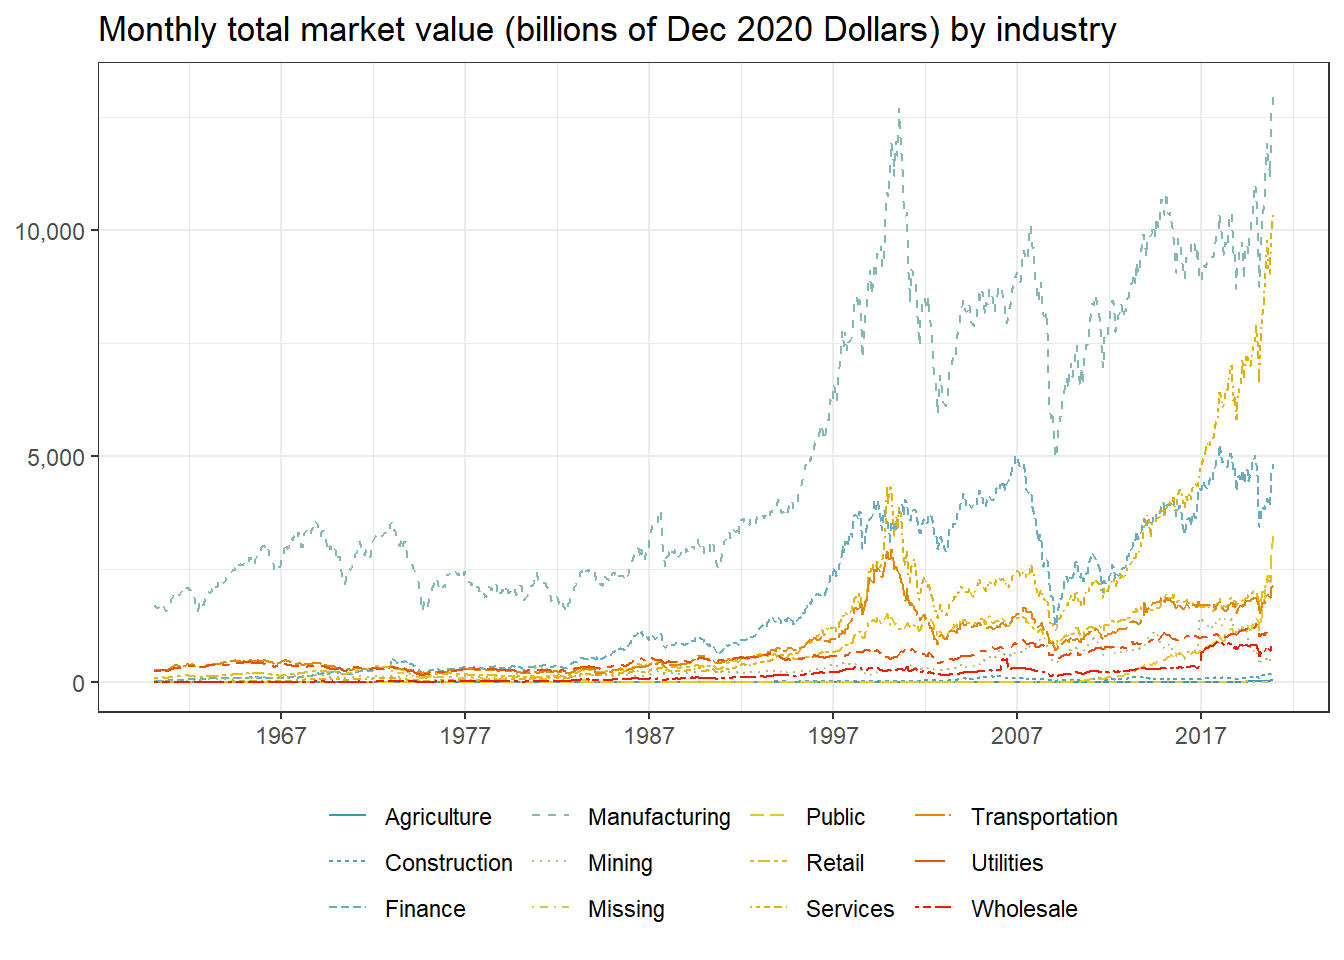
\includegraphics{21_WRDS_files/figure-latex/unnamed-chunk-22-1} \end{center}

We also compute the market value of all stocks belonging to the respective industries. All values are again in terms of billions of end of 2020 dollars. At all points in time, manufacturing firms comprise of the largest portion of market capitalization. Towards the end of the sample, however, financial firms and services begin to make up a substantial portion of the market value.

\begin{Shaded}
\begin{Highlighting}[]
\NormalTok{crsp\_monthly\_industry }\SpecialCharTok{|}\ErrorTok{\textgreater{}}
  \FunctionTok{ggplot}\NormalTok{(}\FunctionTok{aes}\NormalTok{(}\AttributeTok{x =}\NormalTok{ month, }
             \AttributeTok{y =}\NormalTok{ mktcap }\SpecialCharTok{/} \DecValTok{1000}\NormalTok{, }
             \AttributeTok{color =}\NormalTok{ industry, }
             \AttributeTok{linetype =}\NormalTok{ industry)) }\SpecialCharTok{+}
  \FunctionTok{geom\_line}\NormalTok{() }\SpecialCharTok{+}
  \FunctionTok{labs}\NormalTok{(}
    \AttributeTok{x =} \ConstantTok{NULL}\NormalTok{, }\AttributeTok{y =} \ConstantTok{NULL}\NormalTok{, }\AttributeTok{color =} \ConstantTok{NULL}\NormalTok{, }\AttributeTok{linetype =} \ConstantTok{NULL}\NormalTok{,}
    \AttributeTok{title =} \StringTok{"Monthly total market value (billions of Dec 2020 Dollars) by industry"}
\NormalTok{  ) }\SpecialCharTok{+}
  \FunctionTok{scale\_x\_date}\NormalTok{(}\AttributeTok{date\_breaks =} \StringTok{"10 years"}\NormalTok{, }\AttributeTok{date\_labels =} \StringTok{"\%Y"}\NormalTok{) }\SpecialCharTok{+}
  \FunctionTok{scale\_y\_continuous}\NormalTok{(}\AttributeTok{labels =}\NormalTok{ comma)}
\end{Highlighting}
\end{Shaded}

\begin{center}\includegraphics{21_WRDS_files/figure-latex/unnamed-chunk-23-1} \end{center}

\hypertarget{daily-crsp-data}{%
\section{Daily CRSP data}\label{daily-crsp-data}}

Before we turn to accounting data, we also want to provide a proposal for downloading daily CRSP data. While the monthly data from above typically fit into your memory and can be downloaded in a meaningful amount of time, this is usually not true for daily return data. The daily CRSP data file is substantially larger than monthly data and can exceed 20GB. This has two important implications: You cannot hold all the daily return data in your memory (hence it is not possible to copy the entire data set to your local database), and in our experience, the download usually crashes (or never stops) because it is too much data for the WRDS cloud to prepare and send to your R session.

There is a solution to this challenge. As with many `big data' problems, you can split up the big task into several smaller tasks that are easy to handle. That is, instead of downloading data about many stocks all at once, download the data in small batches for each stock consecutively. Such operations can be implemented in \texttt{for} loops, where we download, prepare, and store the data for a single stock in each iteration. This operation might nonetheless take a couple of hours, so you have to be patient either way (we often run such code overnight). To keep track of the progress, you can use \texttt{txtProgressBar()}. Eventually, we end up with more than 68 million rows of daily return data. Note that we only store the identifying information that we actually need, namely \texttt{permno}, \texttt{date}, and \texttt{month} alongside the excess returns. We thus ensure that our local database contains only the data we actually use and that we can load the full daily data into our memory later.

\begin{Shaded}
\begin{Highlighting}[]
\NormalTok{dsf\_db }\OtherTok{\textless{}{-}} \FunctionTok{tbl}\NormalTok{(wrds, }\FunctionTok{in\_schema}\NormalTok{(}\StringTok{"crsp"}\NormalTok{, }\StringTok{"dsf"}\NormalTok{))}
\NormalTok{permnos }\OtherTok{\textless{}{-}} \FunctionTok{tbl}\NormalTok{(tidy\_finance, }\StringTok{"crsp\_monthly"}\NormalTok{) }\SpecialCharTok{|}\ErrorTok{\textgreater{}}
  \FunctionTok{distinct}\NormalTok{(permno) }\SpecialCharTok{|}\ErrorTok{\textgreater{}}
  \FunctionTok{pull}\NormalTok{()}

\NormalTok{progress }\OtherTok{\textless{}{-}} \FunctionTok{txtProgressBar}\NormalTok{(}\AttributeTok{min =} \DecValTok{0}\NormalTok{, }
                           \AttributeTok{max =} \FunctionTok{length}\NormalTok{(permnos), }
                           \AttributeTok{initial =} \DecValTok{0}\NormalTok{, }
                           \AttributeTok{style =} \DecValTok{3}\NormalTok{)}
\ControlFlowTok{for}\NormalTok{ (j }\ControlFlowTok{in} \DecValTok{1}\SpecialCharTok{:}\FunctionTok{length}\NormalTok{(permnos)) \{}
\NormalTok{  permno\_sub }\OtherTok{\textless{}{-}}\NormalTok{ permnos[j]}
\NormalTok{  crsp\_daily\_sub }\OtherTok{\textless{}{-}}\NormalTok{ dsf\_db }\SpecialCharTok{|}\ErrorTok{\textgreater{}}
    \FunctionTok{filter}\NormalTok{(permno }\SpecialCharTok{==}\NormalTok{ permno\_sub }\SpecialCharTok{\&}
\NormalTok{      date }\SpecialCharTok{\textgreater{}=}\NormalTok{ start\_date }\SpecialCharTok{\&}\NormalTok{ date }\SpecialCharTok{\textless{}=}\NormalTok{ end\_date) }\SpecialCharTok{|}\ErrorTok{\textgreater{}}
    \FunctionTok{select}\NormalTok{(permno, date, ret) }\SpecialCharTok{|}\ErrorTok{\textgreater{}}
    \FunctionTok{collect}\NormalTok{() }\SpecialCharTok{|}\ErrorTok{\textgreater{}}
    \FunctionTok{drop\_na}\NormalTok{()}

  \ControlFlowTok{if}\NormalTok{ (}\FunctionTok{nrow}\NormalTok{(crsp\_daily\_sub)) \{}
\NormalTok{    crsp\_daily\_sub }\OtherTok{\textless{}{-}}\NormalTok{ crsp\_daily\_sub }\SpecialCharTok{|}\ErrorTok{\textgreater{}}
      \FunctionTok{mutate}\NormalTok{(}\AttributeTok{month =} \FunctionTok{floor\_date}\NormalTok{(date, }\StringTok{"month"}\NormalTok{)) }\SpecialCharTok{|}\ErrorTok{\textgreater{}}
      \FunctionTok{left\_join}\NormalTok{(factors\_ff\_daily }\SpecialCharTok{|}\ErrorTok{\textgreater{}}
        \FunctionTok{select}\NormalTok{(date, rf), }\AttributeTok{by =} \StringTok{"date"}\NormalTok{) }\SpecialCharTok{|}\ErrorTok{\textgreater{}}
      \FunctionTok{mutate}\NormalTok{(}
        \AttributeTok{ret\_excess =}\NormalTok{ ret }\SpecialCharTok{{-}}\NormalTok{ rf,}
        \AttributeTok{ret\_excess =} \FunctionTok{pmax}\NormalTok{(ret\_excess, }\SpecialCharTok{{-}}\DecValTok{1}\NormalTok{)}
\NormalTok{      ) }\SpecialCharTok{|}\ErrorTok{\textgreater{}}
      \FunctionTok{select}\NormalTok{(permno, date, month, ret\_excess)}

    \ControlFlowTok{if}\NormalTok{ (j }\SpecialCharTok{==} \DecValTok{1}\NormalTok{) \{}
\NormalTok{      overwrite }\OtherTok{\textless{}{-}} \ConstantTok{TRUE}
\NormalTok{      append }\OtherTok{\textless{}{-}} \ConstantTok{FALSE}
\NormalTok{    \} }\ControlFlowTok{else}\NormalTok{ \{}
\NormalTok{      overwrite }\OtherTok{\textless{}{-}} \ConstantTok{FALSE}
\NormalTok{      append }\OtherTok{\textless{}{-}} \ConstantTok{TRUE}
\NormalTok{    \}}

\NormalTok{    crsp\_daily\_sub }\SpecialCharTok{|}\ErrorTok{\textgreater{}}
      \FunctionTok{dbWriteTable}\NormalTok{(tidy\_finance, }
                   \StringTok{"crsp\_daily"}\NormalTok{, }
                   \AttributeTok{value =}\NormalTok{ \_, }
                   \AttributeTok{overwrite =}\NormalTok{ overwrite, }
                   \AttributeTok{append =}\NormalTok{ append)}
\NormalTok{  \}}
  \FunctionTok{setTxtProgressBar}\NormalTok{(progress, j)}
\NormalTok{\}}
\FunctionTok{close}\NormalTok{(progress)}

\NormalTok{crsp\_daily\_db }\OtherTok{\textless{}{-}} \FunctionTok{tbl}\NormalTok{(tidy\_finance, }\StringTok{"crsp\_daily"}\NormalTok{)}
\end{Highlighting}
\end{Shaded}

\hypertarget{preparing-compustat-data}{%
\section{Preparing Compustat data}\label{preparing-compustat-data}}

Firm accounting data are an important source of information that we use in portfolio analyses in subsequent chapters. The commonly used source for firm financial information is Compustat provided by \href{https://www.spglobal.com/marketintelligence/en/}{S\&P Global Market Intelligence}, which is a global data vendor that provides financial, statistical, and market information on active and inactive companies throughout the world. For US and Canadian companies, annual history is available back to 1950 and quarterly as well as monthly histories date back to 1962.

To access Compustat data, we can again tap WRDS, which hosts the \texttt{funda} table that contains annual firm-level information on North American companies.

\begin{Shaded}
\begin{Highlighting}[]
\NormalTok{funda\_db }\OtherTok{\textless{}{-}} \FunctionTok{tbl}\NormalTok{(wrds, }\FunctionTok{in\_schema}\NormalTok{(}\StringTok{"comp"}\NormalTok{, }\StringTok{"funda"}\NormalTok{))}
\end{Highlighting}
\end{Shaded}

We follow the typical filter conventions and pull only data that we actually need: (i) we get only industrial fundamental data (i.e., ignore financial services) (ii) in the standard format (i.e., consolidated information in standard presentation), and (iii) only data in the desired time window.

\begin{Shaded}
\begin{Highlighting}[]
\NormalTok{compustat }\OtherTok{\textless{}{-}}\NormalTok{ funda\_db }\SpecialCharTok{|}\ErrorTok{\textgreater{}}
  \FunctionTok{filter}\NormalTok{(}
\NormalTok{    indfmt }\SpecialCharTok{==} \StringTok{"INDL"} \SpecialCharTok{\&}
\NormalTok{      datafmt }\SpecialCharTok{==} \StringTok{"STD"} \SpecialCharTok{\&}
\NormalTok{      consol }\SpecialCharTok{==} \StringTok{"C"} \SpecialCharTok{\&}
\NormalTok{      datadate }\SpecialCharTok{\textgreater{}=}\NormalTok{ start\_date }\SpecialCharTok{\&}\NormalTok{ datadate }\SpecialCharTok{\textless{}=}\NormalTok{ end\_date}
\NormalTok{  ) }\SpecialCharTok{|}\ErrorTok{\textgreater{}}
  \FunctionTok{select}\NormalTok{(}
\NormalTok{    gvkey, }\CommentTok{\# Firm identifier}
\NormalTok{    datadate, }\CommentTok{\# Date of the accounting data}
\NormalTok{    seq, }\CommentTok{\# Stockholders\textquotesingle{} equity}
\NormalTok{    ceq, }\CommentTok{\# Total common/ordinary equity}
\NormalTok{    at, }\CommentTok{\# Total assets}
\NormalTok{    lt, }\CommentTok{\# Total liabilities}
\NormalTok{    txditc, }\CommentTok{\# Deferred taxes and investment tax credit}
\NormalTok{    txdb, }\CommentTok{\# Deferred taxes}
\NormalTok{    itcb, }\CommentTok{\# Investment tax credit}
\NormalTok{    pstkrv, }\CommentTok{\# Preferred stock redemption value}
\NormalTok{    pstkl, }\CommentTok{\# Preferred stock liquidating value}
\NormalTok{    pstk }\CommentTok{\# Preferred stock par value}
\NormalTok{  ) }\SpecialCharTok{|}\ErrorTok{\textgreater{}}
  \FunctionTok{collect}\NormalTok{()}
\end{Highlighting}
\end{Shaded}

Next, we calculate the book value of preferred stock and equity inspired by the \href{https://mba.tuck.dartmouth.edu/pages/faculty/ken.french/Data_Library/variable_definitions.html}{variable definition in Ken French's data library}. Note that we set negative or zero equity to missing as it makes conceptually little sense (i.e., the firm would be bankrupt).

\begin{Shaded}
\begin{Highlighting}[]
\NormalTok{compustat }\OtherTok{\textless{}{-}}\NormalTok{ compustat }\SpecialCharTok{|}\ErrorTok{\textgreater{}}
  \FunctionTok{mutate}\NormalTok{(}
    \AttributeTok{be =} \FunctionTok{coalesce}\NormalTok{(seq, ceq }\SpecialCharTok{+}\NormalTok{ pstk, at }\SpecialCharTok{{-}}\NormalTok{ lt) }\SpecialCharTok{+}
      \FunctionTok{coalesce}\NormalTok{(txditc, txdb }\SpecialCharTok{+}\NormalTok{ itcb, }\DecValTok{0}\NormalTok{) }\SpecialCharTok{{-}}
      \FunctionTok{coalesce}\NormalTok{(pstkrv, pstkl, pstk, }\DecValTok{0}\NormalTok{),}
    \AttributeTok{be =} \FunctionTok{if\_else}\NormalTok{(be }\SpecialCharTok{\textless{}=} \DecValTok{0}\NormalTok{, }\FunctionTok{as.numeric}\NormalTok{(}\ConstantTok{NA}\NormalTok{), be)}
\NormalTok{  )}
\end{Highlighting}
\end{Shaded}

We keep only the last available information for each firm-year group. Note that \texttt{datadate} defines the time the corresponding financial data refers to (e.g., annual report as of December 31, 2020). Therefore, \texttt{datadate} is not the date when data was made available to the public. Check out the exercises for more insights into the peculiarities of \texttt{datadate}.

\begin{Shaded}
\begin{Highlighting}[]
\NormalTok{compustat }\OtherTok{\textless{}{-}}\NormalTok{ compustat }\SpecialCharTok{|}\ErrorTok{\textgreater{}}
  \FunctionTok{mutate}\NormalTok{(}\AttributeTok{year =} \FunctionTok{year}\NormalTok{(datadate)) }\SpecialCharTok{|}\ErrorTok{\textgreater{}}
  \FunctionTok{group\_by}\NormalTok{(gvkey, year) }\SpecialCharTok{|}\ErrorTok{\textgreater{}}
  \FunctionTok{filter}\NormalTok{(datadate }\SpecialCharTok{==} \FunctionTok{max}\NormalTok{(datadate)) }\SpecialCharTok{|}\ErrorTok{\textgreater{}}
  \FunctionTok{ungroup}\NormalTok{()}
\end{Highlighting}
\end{Shaded}

With the last step, we are already done preparing the firm fundamentals. Thus, we can store them in our local database.

\begin{Shaded}
\begin{Highlighting}[]
\NormalTok{compustat }\SpecialCharTok{|}\ErrorTok{\textgreater{}}
  \FunctionTok{dbWriteTable}\NormalTok{(tidy\_finance, }
               \StringTok{"compustat"}\NormalTok{, }
               \AttributeTok{value =}\NormalTok{ \_, }
               \AttributeTok{overwrite =} \ConstantTok{TRUE}\NormalTok{)}
\end{Highlighting}
\end{Shaded}

\hypertarget{merging-crsp-with-compustat}{%
\section{Merging CRSP with Compustat}\label{merging-crsp-with-compustat}}

Unfortunately, CRSP and Compustat use different keys to identify stocks and firms. CRSP uses \texttt{permno} for stocks, while Compustat uses \texttt{gvkey} to identify firms. Fortunately, a curated matching table on WRDS allows us to merge CRSP and Compustat, so we create a connection to the \emph{CRSP-Compustat Merged} table (provided by CRSP).

\begin{Shaded}
\begin{Highlighting}[]
\NormalTok{ccmxpf\_linktable\_db }\OtherTok{\textless{}{-}} \FunctionTok{tbl}\NormalTok{(wrds, }
                           \FunctionTok{in\_schema}\NormalTok{(}\StringTok{"crsp"}\NormalTok{, }\StringTok{"ccmxpf\_linktable"}\NormalTok{))}
\end{Highlighting}
\end{Shaded}

The linking table contains links between CRSP and Compustat identifiers from various approaches. However, we need to make sure that we keep only relevant and correct links, again following the description outlined in BEM. Note also that currently active links have no end date, so we just enter the current date via \texttt{Sys.Date()}.

\begin{Shaded}
\begin{Highlighting}[]
\NormalTok{ccmxpf\_linktable }\OtherTok{\textless{}{-}}\NormalTok{ ccmxpf\_linktable\_db }\SpecialCharTok{|}\ErrorTok{\textgreater{}}
  \FunctionTok{filter}\NormalTok{(linktype }\SpecialCharTok{\%in\%} \FunctionTok{c}\NormalTok{(}\StringTok{"LU"}\NormalTok{, }\StringTok{"LC"}\NormalTok{) }\SpecialCharTok{\&}
\NormalTok{    linkprim }\SpecialCharTok{\%in\%} \FunctionTok{c}\NormalTok{(}\StringTok{"P"}\NormalTok{, }\StringTok{"C"}\NormalTok{) }\SpecialCharTok{\&}
\NormalTok{    usedflag }\SpecialCharTok{==} \DecValTok{1}\NormalTok{) }\SpecialCharTok{|}\ErrorTok{\textgreater{}}
  \FunctionTok{select}\NormalTok{(}\AttributeTok{permno =}\NormalTok{ lpermno, gvkey, linkdt, linkenddt) }\SpecialCharTok{|}\ErrorTok{\textgreater{}}
  \FunctionTok{collect}\NormalTok{() }\SpecialCharTok{|}\ErrorTok{\textgreater{}}
  \FunctionTok{mutate}\NormalTok{(}\AttributeTok{linkenddt =} \FunctionTok{replace\_na}\NormalTok{(linkenddt, }\FunctionTok{Sys.Date}\NormalTok{()))}
\NormalTok{ccmxpf\_linktable}
\end{Highlighting}
\end{Shaded}

\begin{verbatim}
## # A tibble: 31,770 x 4
##   permno gvkey  linkdt     linkenddt 
##    <dbl> <chr>  <date>     <date>    
## 1  25881 001000 1970-11-13 1978-06-30
## 2  10015 001001 1983-09-20 1986-07-31
## 3  10023 001002 1972-12-14 1973-06-05
## 4  10031 001003 1983-12-07 1989-08-16
## 5  54594 001004 1972-04-24 2022-07-11
## # ... with 31,765 more rows
\end{verbatim}

We use these links to create a new table with a mapping between stock identifier, firm identifier, and month. We then add these links to the Compustat \texttt{gvkey} to our monthly stock data.

\begin{Shaded}
\begin{Highlighting}[]
\NormalTok{ccm\_links }\OtherTok{\textless{}{-}}\NormalTok{ crsp\_monthly }\SpecialCharTok{|}\ErrorTok{\textgreater{}}
  \FunctionTok{inner\_join}\NormalTok{(ccmxpf\_linktable, }\AttributeTok{by =} \StringTok{"permno"}\NormalTok{) }\SpecialCharTok{|}\ErrorTok{\textgreater{}}
  \FunctionTok{filter}\NormalTok{(}\SpecialCharTok{!}\FunctionTok{is.na}\NormalTok{(gvkey) }\SpecialCharTok{\&}\NormalTok{ (date }\SpecialCharTok{\textgreater{}=}\NormalTok{ linkdt }\SpecialCharTok{\&}\NormalTok{ date }\SpecialCharTok{\textless{}=}\NormalTok{ linkenddt)) }\SpecialCharTok{|}\ErrorTok{\textgreater{}}
  \FunctionTok{select}\NormalTok{(permno, gvkey, date)}

\NormalTok{crsp\_monthly }\OtherTok{\textless{}{-}}\NormalTok{ crsp\_monthly }\SpecialCharTok{|}\ErrorTok{\textgreater{}}
  \FunctionTok{left\_join}\NormalTok{(ccm\_links, }\AttributeTok{by =} \FunctionTok{c}\NormalTok{(}\StringTok{"permno"}\NormalTok{, }\StringTok{"date"}\NormalTok{))}
\end{Highlighting}
\end{Shaded}

As the last step, we update the previously prepared monthly CRSP file with the linking information in our local database.

\begin{Shaded}
\begin{Highlighting}[]
\NormalTok{crsp\_monthly }\SpecialCharTok{|}\ErrorTok{\textgreater{}}
  \FunctionTok{dbWriteTable}\NormalTok{(tidy\_finance, }
               \StringTok{"crsp\_monthly"}\NormalTok{, }
               \AttributeTok{value =}\NormalTok{ \_, }
               \AttributeTok{overwrite =} \ConstantTok{TRUE}\NormalTok{)}
\end{Highlighting}
\end{Shaded}

Before we close this chapter, let us look at an interesting descriptive statistic of our data. As the book value of equity plays a crucial role in many asset pricing applications, it is interesting to know for how many of our stocks this information is available. Hence, the figure below plots the share of securities with book equity values for each exchange. It turns out that the coverage is pretty bad for AMEX- and NYSE-listed stocks in the 60s but hovers around 80\% for all periods thereafter. We can ignore the erratic coverage of securities that belong to the other category since there is only a handful of them anyway in our sample.

\begin{Shaded}
\begin{Highlighting}[]
\NormalTok{crsp\_monthly }\SpecialCharTok{|}\ErrorTok{\textgreater{}}
  \FunctionTok{group\_by}\NormalTok{(permno, }\AttributeTok{year =} \FunctionTok{year}\NormalTok{(month)) }\SpecialCharTok{|}\ErrorTok{\textgreater{}}
  \FunctionTok{filter}\NormalTok{(date }\SpecialCharTok{==} \FunctionTok{max}\NormalTok{(date)) }\SpecialCharTok{|}\ErrorTok{\textgreater{}}
  \FunctionTok{ungroup}\NormalTok{() }\SpecialCharTok{|}\ErrorTok{\textgreater{}}
  \FunctionTok{left\_join}\NormalTok{(compustat, }\AttributeTok{by =} \FunctionTok{c}\NormalTok{(}\StringTok{"gvkey"}\NormalTok{, }\StringTok{"year"}\NormalTok{)) }\SpecialCharTok{|}\ErrorTok{\textgreater{}}
  \FunctionTok{group\_by}\NormalTok{(exchange, year) }\SpecialCharTok{|}\ErrorTok{\textgreater{}}
  \FunctionTok{summarize}\NormalTok{(}\AttributeTok{share =} \FunctionTok{n\_distinct}\NormalTok{(permno[}\SpecialCharTok{!}\FunctionTok{is.na}\NormalTok{(be)]) }\SpecialCharTok{/} \FunctionTok{n\_distinct}\NormalTok{(permno),}
            \AttributeTok{.groups =} \StringTok{\textquotesingle{}drop\textquotesingle{}}\NormalTok{) }\SpecialCharTok{|}\ErrorTok{\textgreater{}}
  \FunctionTok{ggplot}\NormalTok{(}\FunctionTok{aes}\NormalTok{(}\AttributeTok{x =}\NormalTok{ year, }\AttributeTok{y =}\NormalTok{ share, }\AttributeTok{color =}\NormalTok{ exchange)) }\SpecialCharTok{+}
  \FunctionTok{geom\_line}\NormalTok{() }\SpecialCharTok{+}
  \FunctionTok{labs}\NormalTok{(}
    \AttributeTok{x =} \ConstantTok{NULL}\NormalTok{, }\AttributeTok{y =} \ConstantTok{NULL}\NormalTok{, }\AttributeTok{color =} \ConstantTok{NULL}\NormalTok{, }\AttributeTok{linetype =} \ConstantTok{NULL}\NormalTok{,}
    \AttributeTok{title =} \StringTok{"End{-}of{-}year share of securities with book equity values by exchange"}
\NormalTok{  ) }\SpecialCharTok{+}
  \FunctionTok{scale\_y\_continuous}\NormalTok{(}\AttributeTok{labels =}\NormalTok{ percent) }\SpecialCharTok{+} 
  \FunctionTok{coord\_cartesian}\NormalTok{(}\AttributeTok{ylim =} \FunctionTok{c}\NormalTok{(}\DecValTok{0}\NormalTok{, }\DecValTok{1}\NormalTok{))}
\end{Highlighting}
\end{Shaded}

\begin{center}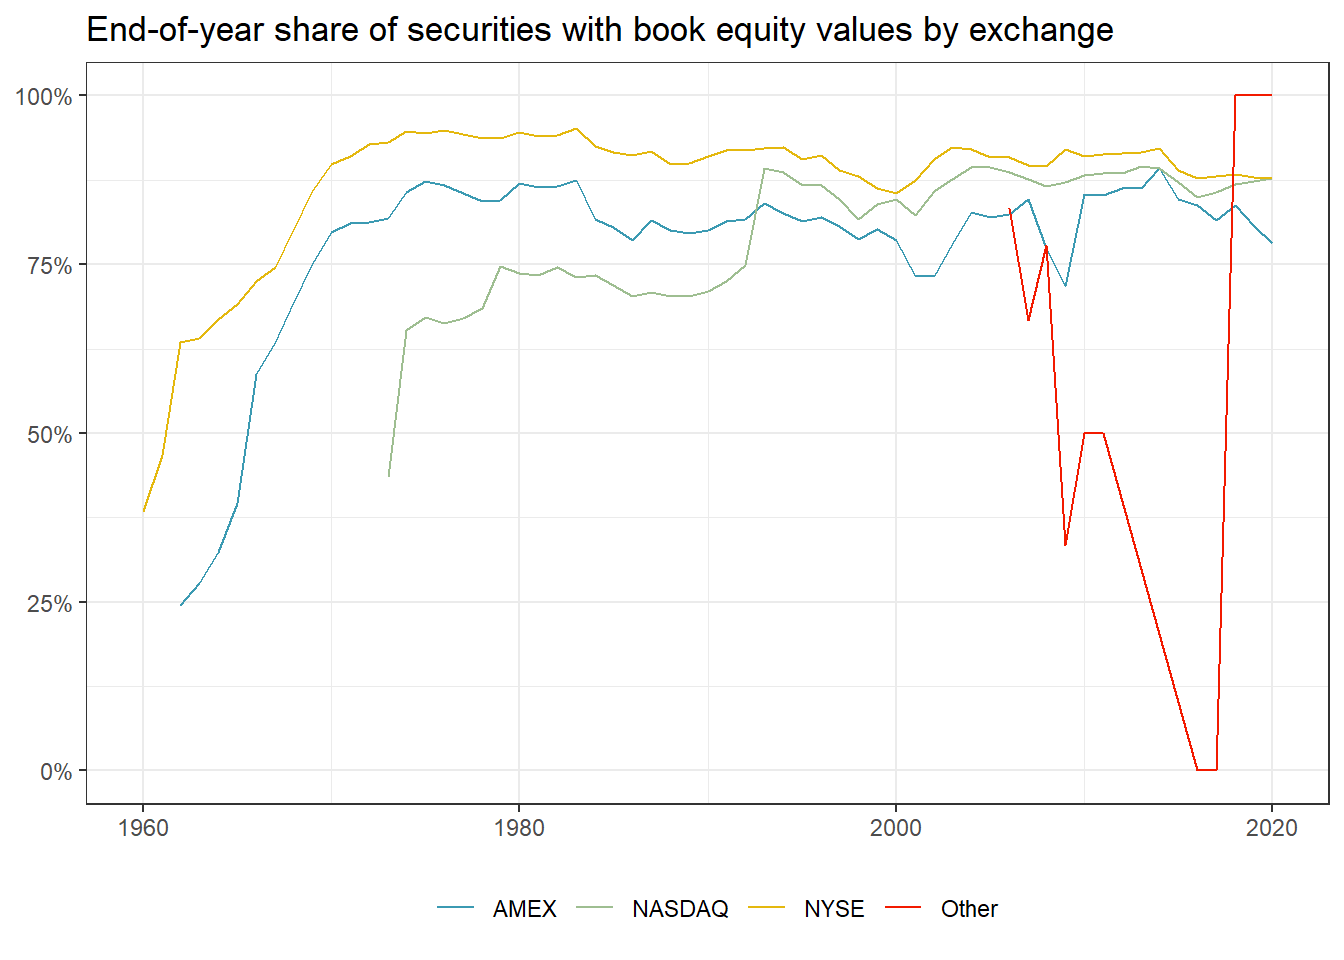
\includegraphics{21_WRDS_files/figure-latex/unnamed-chunk-34-1} \end{center}

\hypertarget{exercises-2}{%
\section{Exercises}\label{exercises-2}}

\begin{enumerate}
\def\labelenumi{\arabic{enumi}.}
\tightlist
\item
  Check out the structure of the WRDS database by sending queries in the spirit of \href{https://wrds-www.wharton.upenn.edu/pages/support/programming-wrds/programming-r/querying-wrds-data-r/}{``Querying WRDS Data using R''} and verify the output with \texttt{dbListObjects()}. How many tables are associated with CRSP? Can you identify what is stored within \emph{msp500}?
\item
  Compute \texttt{mkt\_cap\_lag} using \texttt{lag(mktcap)} rather than joins as above. Filter out all the rows where the lag-based market capitalization measure is different from the one we computed above. Why are they different?
\item
  In the main part, we look at the distribution of market capitalization across exchanges and industries. Now, plot the average market capitalization of firms for each exchange and industry. What do you find?
\item
  \texttt{datadate} refers to the date to which the fiscal year of a corresponding firm refers to. Count the number of observations in Compustat by \emph{month} of this date variable. What do you find? What does the finding suggest about pooling observations with the same fiscal year?
\item
  Go back to the original Compustat data in \texttt{funda\_db} and extract rows where the same firm has multiple rows for the same fiscal year. What is the reason for these observations?
\item
  Repeat the analysis of market capitalization for book equity, which we computed from the Compustat data. Then, used the matched sample to plot book equity against market capitalization. How are these two variables related?
\end{enumerate}

\hypertarget{part-asset-pricing}{%
\part*{Asset pricing}\label{part-asset-pricing}}


\hypertarget{beta-estimation}{%
\chapter{Beta estimation}\label{beta-estimation}}

In this chapter, we introduce you to an important concept in financial economics: the exposure of an individual stock to changes in the market portfolio. According to the Capital Asset Pricing Model (CAPM), cross-sectional variation in expected asset returns should be a function of the covariance between the excess return of the asset and the excess return on the market portfolio. The regression coefficient of market returns on excess returns is usually called the market beta. We show an estimation procedure for the market betas. We do not go into details about the foundations of market beta but simply refer to any treatment of the \href{https://en.wikipedia.org/wiki/Capital_asset_pricing_model}{CAPM} for further information. Instead, we provide details about all the functions that we use to compute the results. In particular, we leverage useful computational concepts: rolling-window estimation and parallelization.

We use the following packages throughout this chapter:

\begin{Shaded}
\begin{Highlighting}[]
\FunctionTok{library}\NormalTok{(tidyverse)}
\FunctionTok{library}\NormalTok{(RSQLite)}
\FunctionTok{library}\NormalTok{(slider)}
\FunctionTok{library}\NormalTok{(scales)}
\FunctionTok{library}\NormalTok{(furrr)}
\end{Highlighting}
\end{Shaded}

\hypertarget{estimating-beta-using-monthly-returns}{%
\section{Estimating beta using monthly returns}\label{estimating-beta-using-monthly-returns}}

The estimation procedure is based on a rolling-window estimation where we may use either monthly or daily returns and different window lengths. First, let us start with loading the monthly data we prepared in the previous chapter from our \texttt{SQLite}-database introduced in our chapter on \emph{``Accessing \& managing financial data''}.

\begin{Shaded}
\begin{Highlighting}[]
\NormalTok{tidy\_finance }\OtherTok{\textless{}{-}} \FunctionTok{dbConnect}\NormalTok{(}
  \FunctionTok{SQLite}\NormalTok{(), }\StringTok{"data/tidy\_finance.sqlite"}\NormalTok{, }\AttributeTok{extended\_types =} \ConstantTok{TRUE}
\NormalTok{)}

\NormalTok{crsp\_monthly }\OtherTok{\textless{}{-}} \FunctionTok{tbl}\NormalTok{(tidy\_finance, }\StringTok{"crsp\_monthly"}\NormalTok{) }\SpecialCharTok{|}\ErrorTok{\textgreater{}}
  \FunctionTok{collect}\NormalTok{()}

\NormalTok{factors\_ff\_monthly }\OtherTok{\textless{}{-}} \FunctionTok{tbl}\NormalTok{(tidy\_finance, }\StringTok{"factors\_ff\_monthly"}\NormalTok{) }\SpecialCharTok{|}\ErrorTok{\textgreater{}}
  \FunctionTok{collect}\NormalTok{()}

\NormalTok{crsp\_monthly }\OtherTok{\textless{}{-}}\NormalTok{ crsp\_monthly }\SpecialCharTok{|}\ErrorTok{\textgreater{}}
  \FunctionTok{left\_join}\NormalTok{(factors\_ff\_monthly, }\AttributeTok{by =} \StringTok{"month"}\NormalTok{) }\SpecialCharTok{|}\ErrorTok{\textgreater{}}
  \FunctionTok{select}\NormalTok{(permno, month, industry, ret\_excess, mkt\_excess)}
\end{Highlighting}
\end{Shaded}

To estimate the CAPM equation
\[
r_{i, t} - r_{f, t} = \alpha_i + \beta_i(r_{m, t}-r_{f,t})+\varepsilon_{i, t}
\]
we regress excess stock returns \texttt{ret\_excess} on excess returns of the market portfolio \texttt{mkt\_excess}.
R provides a simple solution to estimate (linear) models with the function \texttt{lm()}. \texttt{lm()} requires a formula as input that is specified in a compact symbolic form. An expression of the form \texttt{y\ \textasciitilde{}\ model} is interpreted as a specification that the response \texttt{y} is modeled by a linear predictor specified symbolically by \texttt{model}. Such a model consists of a series of terms separated by \texttt{+} operators. In addition to standard linear models, \texttt{lm()} provides a lot of flexibility. You should check out the documentation for more information. To start, we restrict the data only to the time series of observations in CRSP that correspond to Apple's stock (i.e., to \texttt{permno} 14593 for Apple) and compute \(\alpha_i\) as well as \(\beta_i\).

\begin{Shaded}
\begin{Highlighting}[]
\NormalTok{fit }\OtherTok{\textless{}{-}} \FunctionTok{lm}\NormalTok{(ret\_excess }\SpecialCharTok{\textasciitilde{}}\NormalTok{ mkt\_excess,}
  \AttributeTok{data =}\NormalTok{ crsp\_monthly }\SpecialCharTok{|}\ErrorTok{\textgreater{}}
    \FunctionTok{filter}\NormalTok{(permno }\SpecialCharTok{==} \StringTok{"14593"}\NormalTok{)}
\NormalTok{)}

\FunctionTok{summary}\NormalTok{(fit)}
\end{Highlighting}
\end{Shaded}

\begin{verbatim}
## 
## Call:
## lm(formula = ret_excess ~ mkt_excess, data = filter(crsp_monthly, 
##     permno == "14593"))
## 
## Residuals:
##     Min      1Q  Median      3Q     Max 
## -0.5167 -0.0610  0.0009  0.0643  0.3940 
## 
## Coefficients:
##             Estimate Std. Error t value Pr(>|t|)    
## (Intercept)  0.01051    0.00532    1.98    0.049 *  
## mkt_excess   1.40081    0.11748   11.92   <2e-16 ***
## ---
## Signif. codes:  
## 0 '***' 0.001 '**' 0.01 '*' 0.05 '.' 0.1 ' ' 1
## 
## Residual standard error: 0.115 on 478 degrees of freedom
## Multiple R-squared:  0.229,  Adjusted R-squared:  0.228 
## F-statistic:  142 on 1 and 478 DF,  p-value: <2e-16
\end{verbatim}

\texttt{lm()} returns an object of class \texttt{lm} which contains all information we usually care about with linear models. \texttt{summary()} returns an overview of the estimated parameters. \texttt{coefficients(fit)} would return only the estimated coefficients. The output above indicates that Apple moves excessively with the market as the estimated \(\beta_i\) is above one (\(\hat\beta_i\) = 1.4).

\hypertarget{rolling-window-estimation}{%
\section{Rolling-window estimation}\label{rolling-window-estimation}}

After we estimated the regression coefficients on an example, we scale the estimation of \(\beta_i\) to a whole different level and perform rolling-window estimations for the entire CRSP sample. The following function implements the CAPM regression for a data frame (or a part thereof) containing at least \texttt{min\_obs} observations to avoid huge fluctuations if the time series is too short. If the condition is violated, the function returns a missing value.

\begin{Shaded}
\begin{Highlighting}[]
\NormalTok{estimate\_capm }\OtherTok{\textless{}{-}} \ControlFlowTok{function}\NormalTok{(data, }\AttributeTok{min\_obs =} \DecValTok{1}\NormalTok{) \{}
  \ControlFlowTok{if}\NormalTok{ (}\FunctionTok{nrow}\NormalTok{(data) }\SpecialCharTok{\textless{}}\NormalTok{ min\_obs) \{}
\NormalTok{    beta }\OtherTok{\textless{}{-}} \FunctionTok{as.numeric}\NormalTok{(}\ConstantTok{NA}\NormalTok{)}
\NormalTok{  \} }\ControlFlowTok{else}\NormalTok{ \{}
\NormalTok{    fit }\OtherTok{\textless{}{-}} \FunctionTok{lm}\NormalTok{(ret\_excess }\SpecialCharTok{\textasciitilde{}}\NormalTok{ mkt\_excess, }\AttributeTok{data =}\NormalTok{ data)}
\NormalTok{    beta }\OtherTok{\textless{}{-}} \FunctionTok{as.numeric}\NormalTok{(fit}\SpecialCharTok{$}\NormalTok{coefficients[}\DecValTok{2}\NormalTok{])}
\NormalTok{  \}}
  \FunctionTok{return}\NormalTok{(beta)}
\NormalTok{\}}
\end{Highlighting}
\end{Shaded}

Next, we define a function that does the rolling estimation. To perform the rolling-window estimation, we use the \texttt{slider} package of \href{https://github.com/DavisVaughan/slider}{Davis Vaughan}. The \texttt{slide\_period} function is able to handle months in its window input in a straightforward manner. We thus avoid using any time-series package (e.g., \texttt{zoo}) and converting the data to fit the package functions, but rather stay in the world of tibbles.

The following function takes input data and slides across the month vector, considering only a total of \texttt{months} months. The function essentially performs three steps: (i) combine all rows into a single data frame (which comes in handy in the case of daily data), (ii) compute betas by sliding across months, and (iii) return a tibble with months and corresponding beta estimates (again particularly useful in the case of daily data).
As we demonstrate further below, we can also apply the same function to daily returns data.

\begin{Shaded}
\begin{Highlighting}[]
\NormalTok{roll\_capm\_estimation }\OtherTok{\textless{}{-}} \ControlFlowTok{function}\NormalTok{(data, months, min\_obs) \{}
\NormalTok{  data }\OtherTok{\textless{}{-}} \FunctionTok{bind\_rows}\NormalTok{(data) }\SpecialCharTok{|}\ErrorTok{\textgreater{}}
    \FunctionTok{arrange}\NormalTok{(month)}

\NormalTok{  betas }\OtherTok{\textless{}{-}} \FunctionTok{slide\_period\_vec}\NormalTok{(}
    \AttributeTok{.x =}\NormalTok{ data,}
    \AttributeTok{.i =}\NormalTok{ data}\SpecialCharTok{$}\NormalTok{month,}
    \AttributeTok{.period =} \StringTok{"month"}\NormalTok{,}
    \AttributeTok{.f =} \SpecialCharTok{\textasciitilde{}}\FunctionTok{estimate\_capm}\NormalTok{(., min\_obs),}
    \AttributeTok{.before =}\NormalTok{ months }\SpecialCharTok{{-}} \DecValTok{1}\NormalTok{,}
    \AttributeTok{.complete =} \ConstantTok{FALSE}
\NormalTok{  )}

  \FunctionTok{tibble}\NormalTok{(}
    \AttributeTok{month =} \FunctionTok{unique}\NormalTok{(data}\SpecialCharTok{$}\NormalTok{month),}
    \AttributeTok{beta =}\NormalTok{ betas}
\NormalTok{  )}
\NormalTok{\}}
\end{Highlighting}
\end{Shaded}

Before we attack the whole CRSP sample, let us focus on a couple of examples for well-known firms.

\begin{Shaded}
\begin{Highlighting}[]
\NormalTok{examples }\OtherTok{\textless{}{-}} \FunctionTok{tribble}\NormalTok{(}
  \SpecialCharTok{\textasciitilde{}}\NormalTok{permno, }\SpecialCharTok{\textasciitilde{}}\NormalTok{company,}
  \DecValTok{14593}\NormalTok{, }\StringTok{"Apple"}\NormalTok{,}
  \DecValTok{10107}\NormalTok{, }\StringTok{"Microsoft"}\NormalTok{,}
  \DecValTok{93436}\NormalTok{, }\StringTok{"Tesla"}\NormalTok{,}
  \DecValTok{17778}\NormalTok{, }\StringTok{"Berkshire Hathaway"}
\NormalTok{)}
\end{Highlighting}
\end{Shaded}

If we want to estimate rolling betas for Apple, we can use \texttt{mutate()}.
We take a total of 5 years of data and require at least 48 months with return data to compute our betas.
Check out the exercises if you want ot compute beta for different time periods.

\begin{Shaded}
\begin{Highlighting}[]
\NormalTok{beta\_example }\OtherTok{\textless{}{-}}\NormalTok{ crsp\_monthly }\SpecialCharTok{|}\ErrorTok{\textgreater{}}
  \FunctionTok{filter}\NormalTok{(permno }\SpecialCharTok{==}\NormalTok{ examples}\SpecialCharTok{$}\NormalTok{permno[}\DecValTok{1}\NormalTok{]) }\SpecialCharTok{|}\ErrorTok{\textgreater{}}
  \FunctionTok{mutate}\NormalTok{(}\FunctionTok{roll\_capm\_estimation}\NormalTok{(}\FunctionTok{cur\_data}\NormalTok{(), }\AttributeTok{months =} \DecValTok{60}\NormalTok{, }\AttributeTok{min\_obs =} \DecValTok{48}\NormalTok{)) }\SpecialCharTok{|}\ErrorTok{\textgreater{}}
  \FunctionTok{drop\_na}\NormalTok{()}
\NormalTok{beta\_example}
\end{Highlighting}
\end{Shaded}

\begin{verbatim}
## # A tibble: 433 x 6
##   permno month      industry      ret_excess mkt_excess
##    <dbl> <date>     <chr>              <dbl>      <dbl>
## 1  14593 1984-12-01 Manufacturing     0.170      0.0184
## 2  14593 1985-01-01 Manufacturing    -0.0108     0.0799
## 3  14593 1985-02-01 Manufacturing    -0.152      0.0122
## 4  14593 1985-03-01 Manufacturing    -0.112     -0.0084
## 5  14593 1985-04-01 Manufacturing    -0.0467    -0.0096
## # ... with 428 more rows, and 1 more variable:
## #   beta <dbl>
\end{verbatim}

It is actually quite simple to perform the rolling-window estimation for an arbitrary number of stocks, which we visualize in the following code chunk.

\begin{Shaded}
\begin{Highlighting}[]
\NormalTok{beta\_examples }\OtherTok{\textless{}{-}}\NormalTok{ crsp\_monthly }\SpecialCharTok{|}\ErrorTok{\textgreater{}}
  \FunctionTok{inner\_join}\NormalTok{(examples, }\AttributeTok{by =} \StringTok{"permno"}\NormalTok{) }\SpecialCharTok{|}\ErrorTok{\textgreater{}}
  \FunctionTok{group\_by}\NormalTok{(permno) }\SpecialCharTok{|}\ErrorTok{\textgreater{}}
  \FunctionTok{mutate}\NormalTok{(}\FunctionTok{roll\_capm\_estimation}\NormalTok{(}\FunctionTok{cur\_data}\NormalTok{(), }\AttributeTok{months =} \DecValTok{60}\NormalTok{, }\AttributeTok{min\_obs =} \DecValTok{48}\NormalTok{)) }\SpecialCharTok{|}\ErrorTok{\textgreater{}}
  \FunctionTok{ungroup}\NormalTok{() }\SpecialCharTok{|}\ErrorTok{\textgreater{}}
  \FunctionTok{select}\NormalTok{(permno, company, month, }\AttributeTok{beta\_monthly =}\NormalTok{ beta) }\SpecialCharTok{|}\ErrorTok{\textgreater{}}
  \FunctionTok{drop\_na}\NormalTok{()}

\NormalTok{beta\_examples }\SpecialCharTok{|}\ErrorTok{\textgreater{}}
  \FunctionTok{ggplot}\NormalTok{(}\FunctionTok{aes}\NormalTok{(}\AttributeTok{x =}\NormalTok{ month, }\AttributeTok{y =}\NormalTok{ beta\_monthly, }\AttributeTok{color =}\NormalTok{ company)) }\SpecialCharTok{+}
  \FunctionTok{geom\_line}\NormalTok{() }\SpecialCharTok{+}
  \FunctionTok{labs}\NormalTok{(}
    \AttributeTok{x =} \ConstantTok{NULL}\NormalTok{, }\AttributeTok{y =} \ConstantTok{NULL}\NormalTok{, }\AttributeTok{color =} \ConstantTok{NULL}\NormalTok{,}
    \AttributeTok{title =} \StringTok{"Monthly beta estimates for example stocks using 5 years of data"}
\NormalTok{  )}
\end{Highlighting}
\end{Shaded}

\begin{center}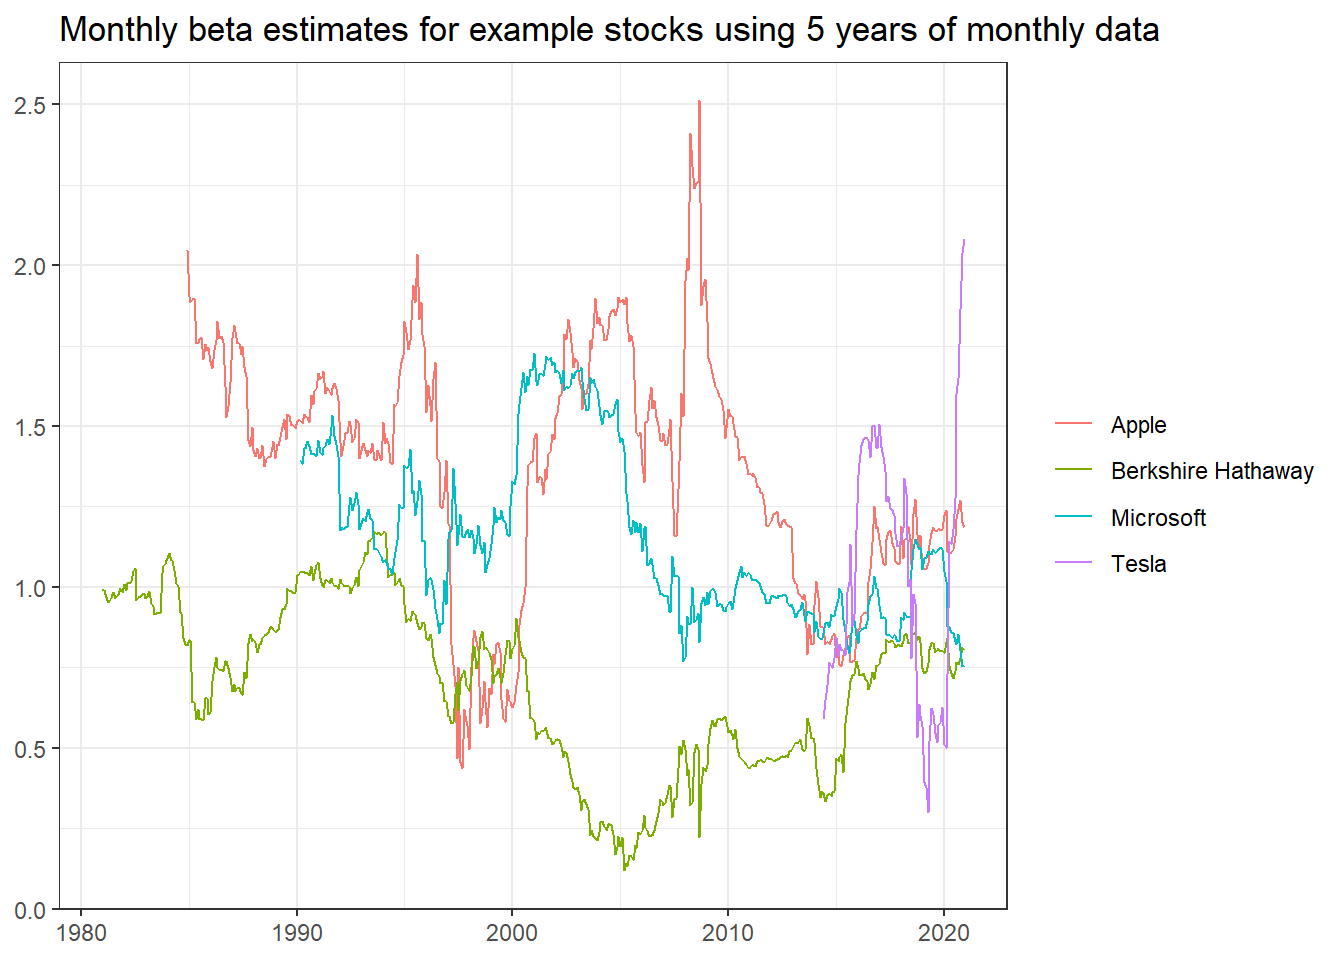
\includegraphics{31_beta_files/figure-latex/unnamed-chunk-8-1} \end{center}

\hypertarget{parallelized-rolling-window-estimation}{%
\section{Parallelized rolling-window estimation}\label{parallelized-rolling-window-estimation}}

Even though we could now just apply the function using \texttt{group\_by()} on the whole CRSP sample, we advise against doing it as it is computationally quite expensive.
Remember that we have to perform rolling-window estimations across all stocks and time periods.
However, this estimation problem is an ideal scenario to employ the power of parallelization.
Parallelization means that we split the tasks which perform rolling-window estimations across different workers (or cores on your local machine).

First, we \texttt{nest()} the data by \texttt{permno}. Nested data means we now have a list of \texttt{permno} with corresponding time series data.

\begin{Shaded}
\begin{Highlighting}[]
\NormalTok{crsp\_monthly\_nested }\OtherTok{\textless{}{-}}\NormalTok{ crsp\_monthly }\SpecialCharTok{|}\ErrorTok{\textgreater{}}
  \FunctionTok{nest}\NormalTok{(}\AttributeTok{data =} \FunctionTok{c}\NormalTok{(month, ret\_excess, mkt\_excess))}
\NormalTok{crsp\_monthly\_nested}
\end{Highlighting}
\end{Shaded}

\begin{verbatim}
## # A tibble: 29,203 x 3
##   permno industry      data              
##    <dbl> <chr>         <list>            
## 1  10000 Manufacturing <tibble [16 x 3]> 
## 2  10001 Utilities     <tibble [378 x 3]>
## 3  10002 Finance       <tibble [324 x 3]>
## 4  10003 Finance       <tibble [118 x 3]>
## 5  10005 Mining        <tibble [65 x 3]> 
## # ... with 29,198 more rows
\end{verbatim}

Next, we ant to apply the \texttt{roll\_capm\_estimation()} function to each stock. This situation is an ideal use case for \texttt{map()}, which takes a list or vector as input and returns an object of the same length as the input. In our case, \texttt{map()} returns a single data frame with a time series of beta estimates for each stock. Therefore, we use \texttt{unnest()} to transform the list of outputs to a tidy data frame.

\begin{Shaded}
\begin{Highlighting}[]
\NormalTok{crsp\_monthly\_nested }\SpecialCharTok{|}\ErrorTok{\textgreater{}}
  \FunctionTok{inner\_join}\NormalTok{(examples, }\AttributeTok{by =} \StringTok{"permno"}\NormalTok{) }\SpecialCharTok{|}\ErrorTok{\textgreater{}}
  \FunctionTok{mutate}\NormalTok{(}\AttributeTok{beta =} \FunctionTok{map}\NormalTok{(}
\NormalTok{    data, }
    \SpecialCharTok{\textasciitilde{}}\FunctionTok{roll\_capm\_estimation}\NormalTok{(., }\AttributeTok{months =} \DecValTok{60}\NormalTok{, }\AttributeTok{min\_obs =} \DecValTok{48}\NormalTok{))}
\NormalTok{    ) }\SpecialCharTok{|}\ErrorTok{\textgreater{}}
  \FunctionTok{unnest}\NormalTok{(}\FunctionTok{c}\NormalTok{(beta)) }\SpecialCharTok{|}\ErrorTok{\textgreater{}}
  \FunctionTok{select}\NormalTok{(permno, month, }\AttributeTok{beta\_monthly =}\NormalTok{ beta) }\SpecialCharTok{|}\ErrorTok{\textgreater{}}
  \FunctionTok{drop\_na}\NormalTok{()}
\end{Highlighting}
\end{Shaded}

\begin{verbatim}
## # A tibble: 1,362 x 3
##   permno month      beta_monthly
##    <dbl> <date>            <dbl>
## 1  10107 1990-03-01         1.39
## 2  10107 1990-04-01         1.38
## 3  10107 1990-05-01         1.43
## 4  10107 1990-06-01         1.43
## 5  10107 1990-07-01         1.45
## # ... with 1,357 more rows
\end{verbatim}

However, instead, we want to perform the estimations of rolling betas for different stocks in parallel. We can use the flexibility of the \texttt{future} package, which we use to define how we want to perform the parallel estimation. If you have a Windows machine, it makes most sense to define \texttt{multisession}, which means that separate R processes are running in the background on the same machine to perform the individual jobs. If you check out the documentation of \texttt{plan()}, you can also see other ways to resolve the parallelization.

\begin{Shaded}
\begin{Highlighting}[]
\FunctionTok{plan}\NormalTok{(multisession, }\AttributeTok{workers =} \FunctionTok{availableCores}\NormalTok{())}
\end{Highlighting}
\end{Shaded}

Using eight cores, the estimation for our sample of around 25k stocks takes around 20 minutes. Of course, you can speed up things considerably by having more cores available to share the workload or by having more powerful cores. Notice the difference in the code below? All you need to do is to replace \texttt{map()} with \texttt{future\_map()}.

\begin{Shaded}
\begin{Highlighting}[]
\NormalTok{beta\_monthly }\OtherTok{\textless{}{-}}\NormalTok{ crsp\_monthly\_nested }\SpecialCharTok{|}\ErrorTok{\textgreater{}}
  \FunctionTok{mutate}\NormalTok{(}\AttributeTok{beta =} \FunctionTok{future\_map}\NormalTok{(}
\NormalTok{    data, }\SpecialCharTok{\textasciitilde{}}\FunctionTok{roll\_capm\_estimation}\NormalTok{(., }\AttributeTok{months =} \DecValTok{60}\NormalTok{, }\AttributeTok{min\_obs =} \DecValTok{48}\NormalTok{))}
\NormalTok{    ) }\SpecialCharTok{|}\ErrorTok{\textgreater{}}
  \FunctionTok{unnest}\NormalTok{(}\FunctionTok{c}\NormalTok{(beta)) }\SpecialCharTok{|}\ErrorTok{\textgreater{}}
  \FunctionTok{select}\NormalTok{(permno, month, }\AttributeTok{beta\_monthly =}\NormalTok{ beta) }\SpecialCharTok{|}\ErrorTok{\textgreater{}}
  \FunctionTok{drop\_na}\NormalTok{()}
\end{Highlighting}
\end{Shaded}

\hypertarget{estimating-beta-using-daily-returns}{%
\section{Estimating beta using daily returns}\label{estimating-beta-using-daily-returns}}

Before we provide some descriptive statistics of our beta estimates, we implement the estimation for the daily CRSP sample as well.
Depending on the application, you might either use longer horizon beta estimates based on monthly data or shorter horizon estimates based on daily returns.

First, we load daily CRSP data.
Note that the sample is large compared to the monthly data, so make sure to have enough memory available.

\begin{Shaded}
\begin{Highlighting}[]
\NormalTok{crsp\_daily }\OtherTok{\textless{}{-}} \FunctionTok{tbl}\NormalTok{(tidy\_finance, }\StringTok{"crsp\_daily"}\NormalTok{) }\SpecialCharTok{|}\ErrorTok{\textgreater{}}
  \FunctionTok{collect}\NormalTok{()}
\end{Highlighting}
\end{Shaded}

We also need the daily Fama-French market excess returns.

\begin{Shaded}
\begin{Highlighting}[]
\NormalTok{factors\_ff\_daily }\OtherTok{\textless{}{-}} \FunctionTok{tbl}\NormalTok{(tidy\_finance, }\StringTok{"factors\_ff\_daily"}\NormalTok{) }\SpecialCharTok{|}\ErrorTok{\textgreater{}}
  \FunctionTok{collect}\NormalTok{()}
\end{Highlighting}
\end{Shaded}

We make sure to keep only relevant data to save memory space.
However, note that your machine might not have enough memory to read the whole daily CRSP sample. In this case, we refer you to the exercises and try working with loops as in chapter 2.

\begin{Shaded}
\begin{Highlighting}[]
\NormalTok{crsp\_daily }\OtherTok{\textless{}{-}}\NormalTok{ crsp\_daily }\SpecialCharTok{|}\ErrorTok{\textgreater{}}
  \FunctionTok{inner\_join}\NormalTok{(factors\_ff\_daily, }\AttributeTok{by =} \StringTok{"date"}\NormalTok{) }\SpecialCharTok{|}\ErrorTok{\textgreater{}}
  \FunctionTok{select}\NormalTok{(permno, month, ret\_excess, mkt\_excess)}
\end{Highlighting}
\end{Shaded}

Just like above, we nest the data by \texttt{permno} for parallelization.

\begin{Shaded}
\begin{Highlighting}[]
\NormalTok{crsp\_daily\_nested }\OtherTok{\textless{}{-}}\NormalTok{ crsp\_daily }\SpecialCharTok{|}\ErrorTok{\textgreater{}}
  \FunctionTok{nest}\NormalTok{(}\AttributeTok{data =} \FunctionTok{c}\NormalTok{(month, ret\_excess, mkt\_excess))}
\end{Highlighting}
\end{Shaded}

This is what the estimation looks like for a couple of examples using \texttt{map()}.
For the daily data, we use the same function as above but only take 3 months of data and require at least 50 daily return observations in these months.
These restrictions help us to retrieve somehow smooth coefficient estimates.

\begin{Shaded}
\begin{Highlighting}[]
\NormalTok{crsp\_daily\_nested }\SpecialCharTok{|}\ErrorTok{\textgreater{}}
  \FunctionTok{inner\_join}\NormalTok{(examples, }\AttributeTok{by =} \StringTok{"permno"}\NormalTok{) }\SpecialCharTok{|}\ErrorTok{\textgreater{}}
  \FunctionTok{mutate}\NormalTok{(}\AttributeTok{beta\_daily =} \FunctionTok{map}\NormalTok{(}
\NormalTok{    data, }
    \SpecialCharTok{\textasciitilde{}}\FunctionTok{roll\_capm\_estimation}\NormalTok{(., }\AttributeTok{months =} \DecValTok{3}\NormalTok{, }\AttributeTok{min\_obs =} \DecValTok{50}\NormalTok{))}
\NormalTok{    ) }\SpecialCharTok{|}\ErrorTok{\textgreater{}}
  \FunctionTok{unnest}\NormalTok{(}\FunctionTok{c}\NormalTok{(beta\_daily)) }\SpecialCharTok{|}\ErrorTok{\textgreater{}}
  \FunctionTok{select}\NormalTok{(permno, month, }\AttributeTok{beta\_daily =}\NormalTok{ beta) }\SpecialCharTok{|}\ErrorTok{\textgreater{}}
  \FunctionTok{drop\_na}\NormalTok{()}
\end{Highlighting}
\end{Shaded}

\begin{verbatim}
## # A tibble: 1,543 x 3
##   permno month      beta_daily
##    <dbl> <date>          <dbl>
## 1  10107 1986-05-01      0.898
## 2  10107 1986-06-01      0.906
## 3  10107 1986-07-01      0.822
## 4  10107 1986-08-01      0.900
## 5  10107 1986-09-01      1.01 
## # ... with 1,538 more rows
\end{verbatim}

For the sake of completeness, we tell our session again to use multiple workers for parallelization.

\begin{Shaded}
\begin{Highlighting}[]
\FunctionTok{plan}\NormalTok{(multisession, }\AttributeTok{workers =} \FunctionTok{availableCores}\NormalTok{())}
\end{Highlighting}
\end{Shaded}

The code chunk for beta estimation using daily returns now looks very similar to the one for monthly data. The whole estimation takes around 30 minutes using eight cores and 32gb memory.

\begin{Shaded}
\begin{Highlighting}[]
\NormalTok{beta\_daily }\OtherTok{\textless{}{-}}\NormalTok{ crsp\_daily\_nested }\SpecialCharTok{|}\ErrorTok{\textgreater{}}
  \FunctionTok{mutate}\NormalTok{(}\AttributeTok{beta\_daily =} \FunctionTok{future\_map}\NormalTok{(}
\NormalTok{    data, }\SpecialCharTok{\textasciitilde{}}\FunctionTok{roll\_capm\_estimation}\NormalTok{(., }\AttributeTok{months =} \DecValTok{3}\NormalTok{, }\AttributeTok{min\_obs =} \DecValTok{50}\NormalTok{))}
\NormalTok{    ) }\SpecialCharTok{|}\ErrorTok{\textgreater{}}
  \FunctionTok{unnest}\NormalTok{(}\FunctionTok{c}\NormalTok{(beta\_daily)) }\SpecialCharTok{|}\ErrorTok{\textgreater{}}
  \FunctionTok{select}\NormalTok{(permno, month, }\AttributeTok{beta\_daily =}\NormalTok{ beta) }\SpecialCharTok{|}\ErrorTok{\textgreater{}}
  \FunctionTok{drop\_na}\NormalTok{()}
\end{Highlighting}
\end{Shaded}

\hypertarget{comparing-beta-estimates}{%
\section{Comparing beta estimates}\label{comparing-beta-estimates}}

What is a typical value for stock betas? To get some feeling, we illustrate the dispersion of the estimated \(\hat\beta_i\) across different industries and across time below. The first figure below shows that typical business models across industries imply different exposure to the general market economy. However, there are barely any firms that exhibit a negative exposure to the market factor.

\begin{Shaded}
\begin{Highlighting}[]
\NormalTok{crsp\_monthly }\SpecialCharTok{|}\ErrorTok{\textgreater{}}
  \FunctionTok{left\_join}\NormalTok{(beta\_monthly, }\AttributeTok{by =} \FunctionTok{c}\NormalTok{(}\StringTok{"permno"}\NormalTok{, }\StringTok{"month"}\NormalTok{)) }\SpecialCharTok{|}\ErrorTok{\textgreater{}}
  \FunctionTok{drop\_na}\NormalTok{(beta\_monthly) }\SpecialCharTok{|}\ErrorTok{\textgreater{}}
  \FunctionTok{group\_by}\NormalTok{(industry, permno) }\SpecialCharTok{|}\ErrorTok{\textgreater{}}
  \FunctionTok{summarize}\NormalTok{(}\AttributeTok{beta =} \FunctionTok{mean}\NormalTok{(beta\_monthly)) }\SpecialCharTok{|}\ErrorTok{\textgreater{}}
  \FunctionTok{ggplot}\NormalTok{(}\FunctionTok{aes}\NormalTok{(}\AttributeTok{x =} \FunctionTok{reorder}\NormalTok{(industry, beta, }\AttributeTok{FUN =}\NormalTok{ median), }\AttributeTok{y =}\NormalTok{ beta)) }\SpecialCharTok{+}
  \FunctionTok{geom\_boxplot}\NormalTok{() }\SpecialCharTok{+}
  \FunctionTok{coord\_flip}\NormalTok{() }\SpecialCharTok{+}
  \FunctionTok{labs}\NormalTok{(}
    \AttributeTok{x =} \ConstantTok{NULL}\NormalTok{, }\AttributeTok{y =} \ConstantTok{NULL}\NormalTok{,}
    \AttributeTok{title =} \StringTok{"Average beta estimates by industry"}
\NormalTok{  )}
\end{Highlighting}
\end{Shaded}

\begin{center}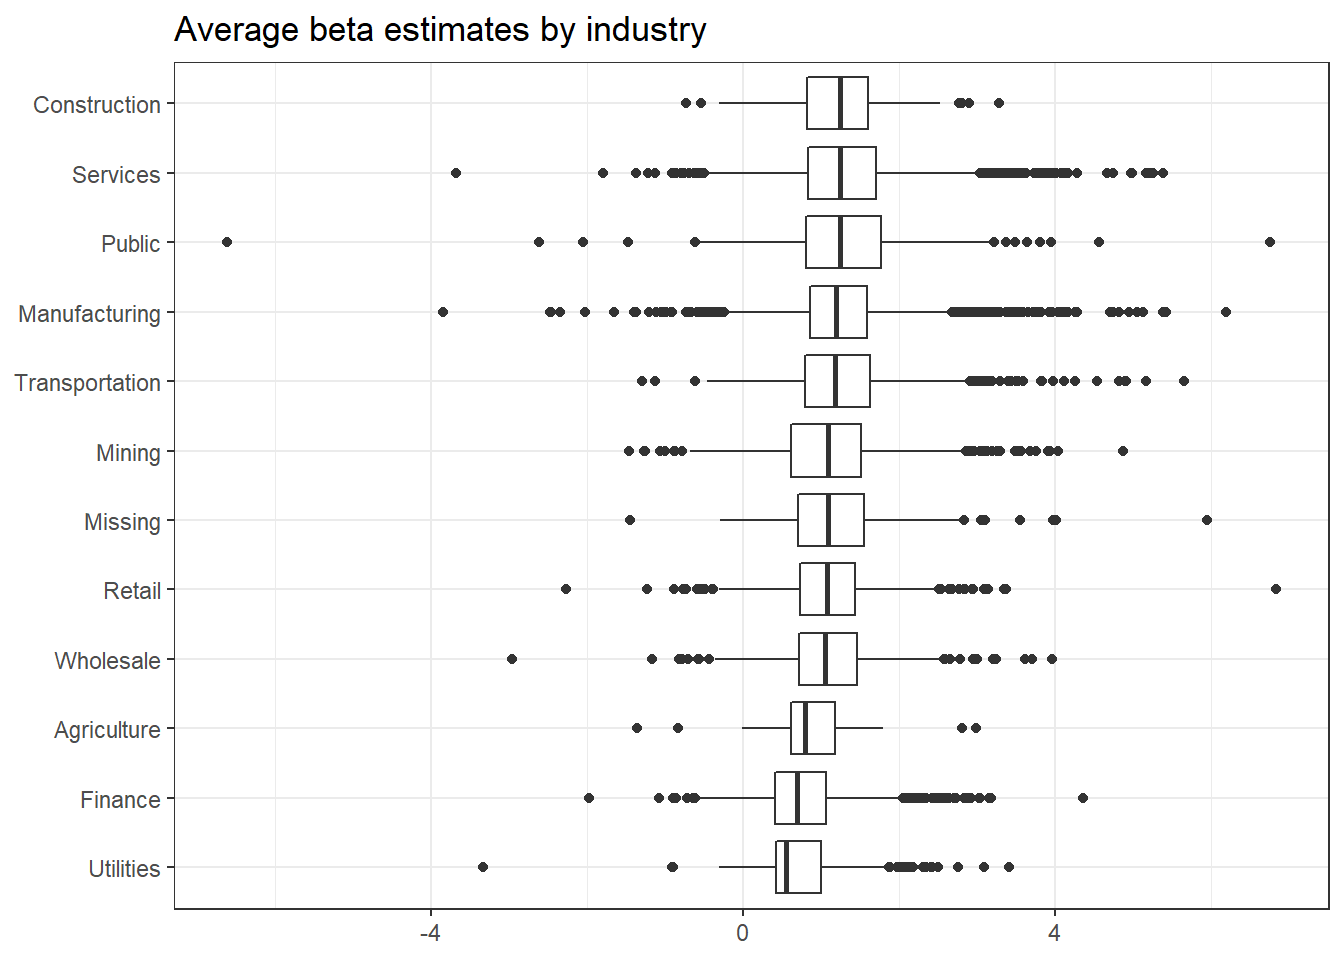
\includegraphics{31_beta_files/figure-latex/unnamed-chunk-19-1} \end{center}

Next, we illustrate the time-variation in the cross-section of estimated betas. The figure below shows the monthly deciles of estimated betas (based on monthly data) and indicates an interesting pattern: First, betas seem to vary over time in the sense that during some periods, there is a clear trend across all deciles. Second, the sample exhibits periods where the dispersion across stocks increases in the sense that the lower decile decreases and the upper decile increases, which indicates that for some stocks the correlation with the market increases while for others it decreases. Note also here: stocks with negative betas are an extremely rare exception.

\begin{Shaded}
\begin{Highlighting}[]
\NormalTok{beta\_monthly }\SpecialCharTok{|}\ErrorTok{\textgreater{}}
  \FunctionTok{drop\_na}\NormalTok{(beta\_monthly) }\SpecialCharTok{|}\ErrorTok{\textgreater{}}
  \FunctionTok{group\_by}\NormalTok{(month) }\SpecialCharTok{|}\ErrorTok{\textgreater{}}
  \FunctionTok{summarize}\NormalTok{(}
    \AttributeTok{x =} \FunctionTok{quantile}\NormalTok{(beta\_monthly, }\FunctionTok{seq}\NormalTok{(}\FloatTok{0.1}\NormalTok{, }\FloatTok{0.9}\NormalTok{, }\FloatTok{0.1}\NormalTok{)),}
    \AttributeTok{quantile =} \DecValTok{100} \SpecialCharTok{*} \FunctionTok{seq}\NormalTok{(}\FloatTok{0.1}\NormalTok{, }\FloatTok{0.9}\NormalTok{, }\FloatTok{0.1}\NormalTok{),}
    \AttributeTok{.groups =} \StringTok{"drop"}
\NormalTok{  ) }\SpecialCharTok{|}\ErrorTok{\textgreater{}}
  \FunctionTok{ggplot}\NormalTok{(}\FunctionTok{aes}\NormalTok{(}\AttributeTok{x =}\NormalTok{ month, }\AttributeTok{y =}\NormalTok{ x, }\AttributeTok{color =} \FunctionTok{as\_factor}\NormalTok{(quantile))) }\SpecialCharTok{+}
  \FunctionTok{geom\_line}\NormalTok{() }\SpecialCharTok{+}
  \FunctionTok{labs}\NormalTok{(}
    \AttributeTok{x =} \ConstantTok{NULL}\NormalTok{, }\AttributeTok{y =} \StringTok{"Beta"}\NormalTok{, }\AttributeTok{color =} \ConstantTok{NULL}\NormalTok{,}
    \AttributeTok{title =} \StringTok{"Distribution of estimated betas"}\NormalTok{,}
    \AttributeTok{subtitle =} \StringTok{"Monthly deciles for CRSP cross{-}section"}
\NormalTok{  )}
\end{Highlighting}
\end{Shaded}

\begin{center}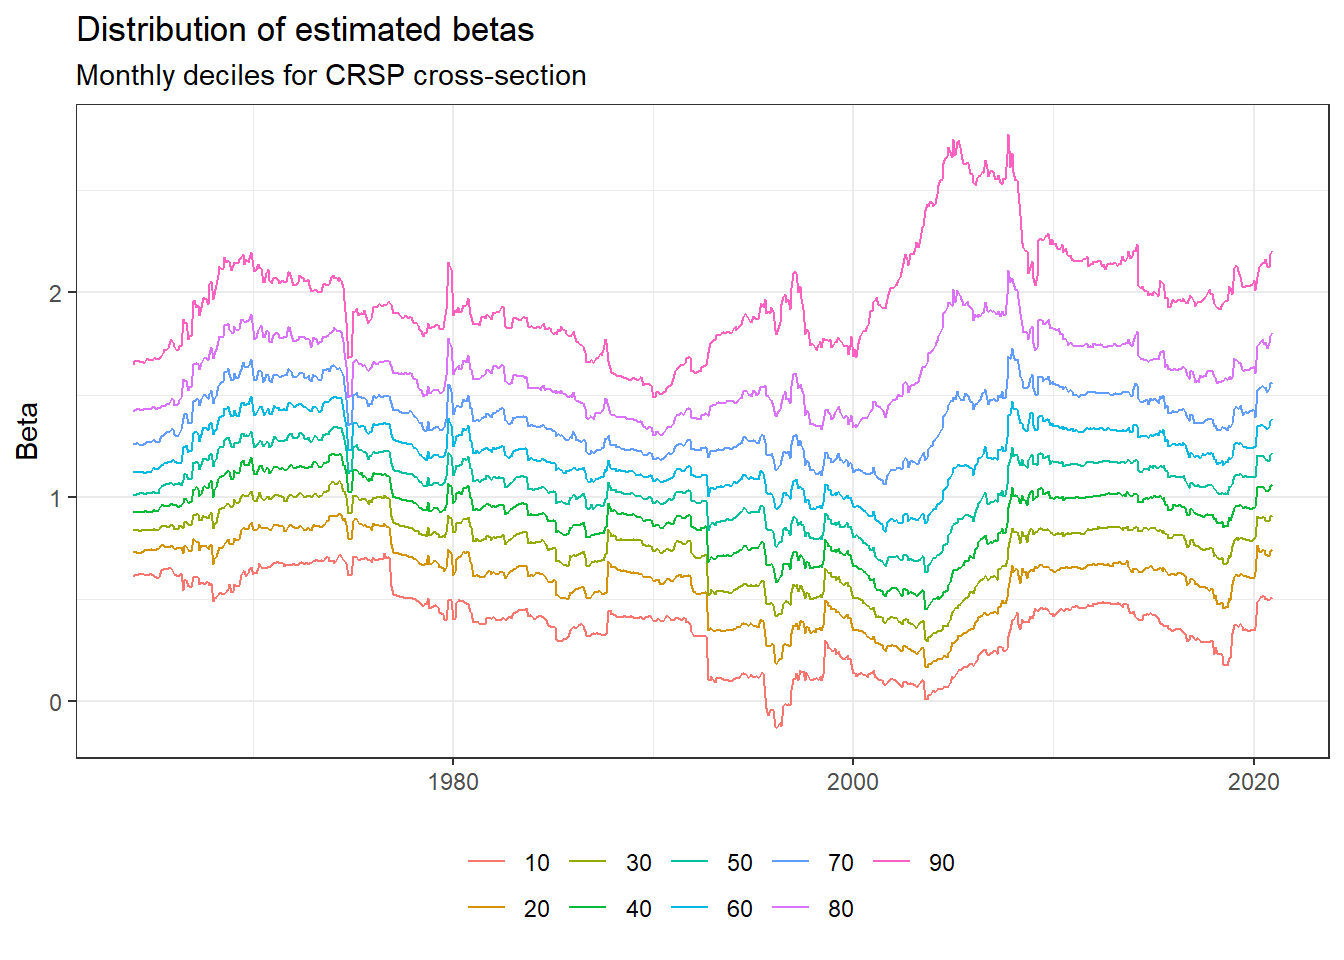
\includegraphics{31_beta_files/figure-latex/unnamed-chunk-20-1} \end{center}

To compare the difference between daily and monthly data, we combine beta estimates to a single table. Then, we use the table to plot a comparison of beta estimates for our example stocks.

\begin{Shaded}
\begin{Highlighting}[]
\NormalTok{beta }\OtherTok{\textless{}{-}}\NormalTok{ beta\_monthly }\SpecialCharTok{|}\ErrorTok{\textgreater{}}
  \FunctionTok{full\_join}\NormalTok{(beta\_daily, }\AttributeTok{by =} \FunctionTok{c}\NormalTok{(}\StringTok{"permno"}\NormalTok{, }\StringTok{"month"}\NormalTok{)) }\SpecialCharTok{|}\ErrorTok{\textgreater{}}
  \FunctionTok{arrange}\NormalTok{(permno, month)}

\NormalTok{beta }\SpecialCharTok{|}\ErrorTok{\textgreater{}}
  \FunctionTok{inner\_join}\NormalTok{(examples, }\AttributeTok{by =} \StringTok{"permno"}\NormalTok{) }\SpecialCharTok{|}\ErrorTok{\textgreater{}}
  \FunctionTok{pivot\_longer}\NormalTok{(}\AttributeTok{cols =} \FunctionTok{c}\NormalTok{(beta\_monthly, beta\_daily)) }\SpecialCharTok{|}\ErrorTok{\textgreater{}}
  \FunctionTok{ggplot}\NormalTok{(}\FunctionTok{aes}\NormalTok{(}\AttributeTok{x =}\NormalTok{ month, }\AttributeTok{y =}\NormalTok{ value, }\AttributeTok{color =}\NormalTok{ name)) }\SpecialCharTok{+}
  \FunctionTok{geom\_line}\NormalTok{() }\SpecialCharTok{+}
  \FunctionTok{facet\_wrap}\NormalTok{(}\SpecialCharTok{\textasciitilde{}}\NormalTok{company, }\AttributeTok{ncol =} \DecValTok{1}\NormalTok{) }\SpecialCharTok{+}
  \FunctionTok{labs}\NormalTok{(}
    \AttributeTok{x =} \ConstantTok{NULL}\NormalTok{, }\AttributeTok{y =} \ConstantTok{NULL}\NormalTok{, }\AttributeTok{color =} \ConstantTok{NULL}\NormalTok{,}
    \AttributeTok{title =} \StringTok{"Comparison of beta estimates using 5 years of monthly and 3 months of daily data"}
\NormalTok{  )}
\end{Highlighting}
\end{Shaded}

\begin{verbatim}
## Warning: Removed 46 row(s) containing missing values
## (geom_path).
\end{verbatim}

\begin{center}\includegraphics{31_beta_files/figure-latex/unnamed-chunk-21-1} \end{center}

The estimates look as expected. As you can see, it really depends on the estimation window and data frequency how your beta estimates turn out.

Finally, we write the estimates to our database such that we can use them in later chapters.

\begin{Shaded}
\begin{Highlighting}[]
\NormalTok{beta }\SpecialCharTok{|}\ErrorTok{\textgreater{}}
  \FunctionTok{dbWriteTable}\NormalTok{(tidy\_finance, }
               \StringTok{"beta"}\NormalTok{, }
               \AttributeTok{value =}\NormalTok{ \_, }
               \AttributeTok{overwrite =} \ConstantTok{TRUE}\NormalTok{)}
\end{Highlighting}
\end{Shaded}

Whenever you perform some kind of estimation, it also makes sense to do rough plausibility tests. A possible check is to plot the share of stocks with beta estimates over time.
This descriptive helps us discover potential errors in our data preparation or estimation procedure.
For instance, suppose there was a gap in our output where we do not have any betas.
In this case, we would have to go back and check all previous steps.

\begin{Shaded}
\begin{Highlighting}[]
\NormalTok{beta\_long }\OtherTok{\textless{}{-}}\NormalTok{ crsp\_monthly }\SpecialCharTok{|}\ErrorTok{\textgreater{}}
  \FunctionTok{left\_join}\NormalTok{(beta, }\AttributeTok{by =} \FunctionTok{c}\NormalTok{(}\StringTok{"permno"}\NormalTok{, }\StringTok{"month"}\NormalTok{)) }\SpecialCharTok{|}\ErrorTok{\textgreater{}}
  \FunctionTok{pivot\_longer}\NormalTok{(}\AttributeTok{cols =} \FunctionTok{c}\NormalTok{(beta\_monthly, beta\_daily))}

\NormalTok{beta\_long }\SpecialCharTok{|}\ErrorTok{\textgreater{}}
  \FunctionTok{group\_by}\NormalTok{(month, name) }\SpecialCharTok{|}\ErrorTok{\textgreater{}}
  \FunctionTok{summarize}\NormalTok{(}\AttributeTok{share =} \FunctionTok{sum}\NormalTok{(}\SpecialCharTok{!}\FunctionTok{is.na}\NormalTok{(value)) }\SpecialCharTok{/} \FunctionTok{n}\NormalTok{()) }\SpecialCharTok{|}\ErrorTok{\textgreater{}}
  \FunctionTok{ggplot}\NormalTok{(}\FunctionTok{aes}\NormalTok{(}\AttributeTok{x =}\NormalTok{ month, }\AttributeTok{y =}\NormalTok{ share, }\AttributeTok{color =}\NormalTok{ name)) }\SpecialCharTok{+}
  \FunctionTok{geom\_line}\NormalTok{() }\SpecialCharTok{+}
  \FunctionTok{scale\_y\_continuous}\NormalTok{(}\AttributeTok{labels =}\NormalTok{ percent) }\SpecialCharTok{+}
  \FunctionTok{labs}\NormalTok{(}
    \AttributeTok{x =} \ConstantTok{NULL}\NormalTok{, }\AttributeTok{y =} \ConstantTok{NULL}\NormalTok{, }\AttributeTok{color =} \ConstantTok{NULL}\NormalTok{,}
    \AttributeTok{title =} \StringTok{"End{-}of{-}month share of securities with beta estimates"}
\NormalTok{  ) }\SpecialCharTok{+}
  \FunctionTok{coord\_cartesian}\NormalTok{(}\AttributeTok{ylim =} \FunctionTok{c}\NormalTok{(}\DecValTok{0}\NormalTok{, }\DecValTok{1}\NormalTok{))}
\end{Highlighting}
\end{Shaded}

\begin{center}\includegraphics{31_beta_files/figure-latex/unnamed-chunk-23-1} \end{center}

The figure above does not indicate any troubles, so let us move on to the next check.

We also encourage everyone to always look at the distributional summary statistics of variables. You can easily spot outliers or weird distributions when looking at such tables.

\begin{Shaded}
\begin{Highlighting}[]
\NormalTok{beta\_long }\SpecialCharTok{|}\ErrorTok{\textgreater{}}
  \FunctionTok{select}\NormalTok{(name, value) }\SpecialCharTok{|}\ErrorTok{\textgreater{}}
  \FunctionTok{drop\_na}\NormalTok{() }\SpecialCharTok{|}\ErrorTok{\textgreater{}}
  \FunctionTok{group\_by}\NormalTok{(name) }\SpecialCharTok{|}\ErrorTok{\textgreater{}}
  \FunctionTok{summarize}\NormalTok{(}
    \AttributeTok{mean =} \FunctionTok{mean}\NormalTok{(value),}
    \AttributeTok{sd =} \FunctionTok{sd}\NormalTok{(value),}
    \AttributeTok{min =} \FunctionTok{min}\NormalTok{(value),}
    \AttributeTok{q05 =} \FunctionTok{quantile}\NormalTok{(value, }\FloatTok{0.05}\NormalTok{),}
    \AttributeTok{q25 =} \FunctionTok{quantile}\NormalTok{(value, }\FloatTok{0.25}\NormalTok{),}
    \AttributeTok{q50 =} \FunctionTok{quantile}\NormalTok{(value, }\FloatTok{0.50}\NormalTok{),}
    \AttributeTok{q75 =} \FunctionTok{quantile}\NormalTok{(value, }\FloatTok{0.75}\NormalTok{),}
    \AttributeTok{q95 =} \FunctionTok{quantile}\NormalTok{(value, }\FloatTok{0.95}\NormalTok{),}
    \AttributeTok{max =} \FunctionTok{max}\NormalTok{(value),}
    \AttributeTok{n =} \FunctionTok{n}\NormalTok{()}
\NormalTok{  )}
\end{Highlighting}
\end{Shaded}

\begin{verbatim}
## # A tibble: 2 x 11
##   name        mean    sd   min    q05   q25   q50   q75
##   <chr>      <dbl> <dbl> <dbl>  <dbl> <dbl> <dbl> <dbl>
## 1 beta_daily 0.743 0.925 -43.7 -0.452 0.203 0.679  1.22
## 2 beta_mont~ 1.10  0.711 -13.0  0.123 0.631 1.03   1.47
## # ... with 3 more variables: q95 <dbl>, max <dbl>,
## #   n <int>
\end{verbatim}

Finally, since we have two different estimators for the same theoretical object, we expect the estimators should be at least positively correlated (although not perfectly as the estimators are based on different sample periods).

\begin{Shaded}
\begin{Highlighting}[]
\NormalTok{beta }\SpecialCharTok{|}\ErrorTok{\textgreater{}}
  \FunctionTok{select}\NormalTok{(beta\_daily, beta\_monthly) }\SpecialCharTok{|}\ErrorTok{\textgreater{}}
  \FunctionTok{cor}\NormalTok{(}\AttributeTok{use =} \StringTok{"complete.obs"}\NormalTok{)}
\end{Highlighting}
\end{Shaded}

\begin{verbatim}
##              beta_daily beta_monthly
## beta_daily        1.000        0.322
## beta_monthly      0.322        1.000
\end{verbatim}

Indeed, we find a positive correlation between our beta estimates. In the subsequent chapters, we mainly use the estimates based on monthly data as most readers should be able to replicate them due to potential memory limitations that might arise with the daily data.

\hypertarget{exercises-3}{%
\section{Exercises}\label{exercises-3}}

\begin{enumerate}
\def\labelenumi{\arabic{enumi}.}
\tightlist
\item
  Compute beta estimates based on monthly data using 1, 3, and 5 years of data and impose a minimum number of observations of 10, 28, and 48 months with return data, respectively. How strongly correlated are the estimated betas?
\item
  Compute beta estimates based on monthly data using 5 years of data and impose different numbers of minimum observations. How does the share of permno-month observations with successful beta estimates vary across the different requirements? Do you find a high correlation across the estimated betas?
\item
  Instead of using \texttt{future\_map()}, perform the beta estimation in a loop (using either monthly or daily data) for a subset of 100 permnos of your choice. Verify that you get the same results as with the parallelized code from above.
\item
  Filter out the stocks with negative betas. Do these stocks frequently exhibit negative betas, or do they resemble estimation errors?
\end{enumerate}

\hypertarget{univariate-portfolio-sorts}{%
\chapter{Univariate portfolio sorts}\label{univariate-portfolio-sorts}}

In this chapter, we dive into portfolio sorts, one of the most widely used statistical methodologies in empirical asset pricing. The key application of portfolio sorts is to examine whether one or more variables can predict future excess returns. In general, the idea is to sort individual stocks into portfolios, where the stocks within each portfolio are similar with respect to a sorting variable, such as firm size. The different portfolios then represent well-diversified investments that differ in the level of the sorting variable. You can then attribute the differences in the return distribution to the impact of the sorting variable.
We start by introducing univariate portfolio sorts (which sort based on only one characteristic). In a later chapter, we tackle bivariate sorting.

A univariate portfolio sort considers only one sorting variable \(x_{t-1,i}\).
Here, \(i\) denotes the stock and \(t-1\) indicates that the characteristic is observable by investors at time \(t\).\\
The objective is to assess the cross-sectional relation between \(x_{t-1,i}\) and, typically, stock excess returns \(r_{t,i}\) at time \(t\) as the outcome variable.
To illustrate how portfolio sorts work, we use estimates for market betas from the previous chapter as our sorting variable.

The current chapter relies on the following set of packages.

\begin{Shaded}
\begin{Highlighting}[]
\FunctionTok{library}\NormalTok{(tidyverse)}
\FunctionTok{library}\NormalTok{(RSQLite)}
\FunctionTok{library}\NormalTok{(lubridate)}
\FunctionTok{library}\NormalTok{(sandwich)}
\FunctionTok{library}\NormalTok{(lmtest)}
\FunctionTok{library}\NormalTok{(scales)}
\end{Highlighting}
\end{Shaded}

\hypertarget{data-preparation}{%
\section{Data preparation}\label{data-preparation}}

We start with loading the required data from our \texttt{SQLite}-database introduced in our chapter on \emph{``Accessing \& managing financial data''}. In particular, we use the monthly CRSP sample as our asset universe.
Once we form our portfolios, we use the Fama-French factor returns to compute the risk-adjusted performance (i.e., alpha).
\texttt{beta} is the tibble with market betas computed in the previous chapter.

\begin{Shaded}
\begin{Highlighting}[]
\NormalTok{tidy\_finance }\OtherTok{\textless{}{-}} \FunctionTok{dbConnect}\NormalTok{(}
  \FunctionTok{SQLite}\NormalTok{(), }\StringTok{"data/tidy\_finance.sqlite"}\NormalTok{, }\AttributeTok{extended\_types =} \ConstantTok{TRUE}
\NormalTok{)}

\NormalTok{crsp\_monthly }\OtherTok{\textless{}{-}} \FunctionTok{tbl}\NormalTok{(tidy\_finance, }\StringTok{"crsp\_monthly"}\NormalTok{) }\SpecialCharTok{|}\ErrorTok{\textgreater{}}
  \FunctionTok{collect}\NormalTok{()}

\NormalTok{factors\_ff\_monthly }\OtherTok{\textless{}{-}} \FunctionTok{tbl}\NormalTok{(tidy\_finance, }\StringTok{"factors\_ff\_monthly"}\NormalTok{) }\SpecialCharTok{|}\ErrorTok{\textgreater{}}
  \FunctionTok{collect}\NormalTok{()}

\NormalTok{beta }\OtherTok{\textless{}{-}} \FunctionTok{tbl}\NormalTok{(tidy\_finance, }\StringTok{"beta"}\NormalTok{) }\SpecialCharTok{|}\ErrorTok{\textgreater{}}
  \FunctionTok{collect}\NormalTok{()}
\end{Highlighting}
\end{Shaded}

We keep only relevant data from the CRSP sample.

\begin{Shaded}
\begin{Highlighting}[]
\NormalTok{crsp\_monthly }\OtherTok{\textless{}{-}}\NormalTok{ crsp\_monthly }\SpecialCharTok{|}\ErrorTok{\textgreater{}}
  \FunctionTok{left\_join}\NormalTok{(factors\_ff\_monthly, }\AttributeTok{by =} \StringTok{"month"}\NormalTok{) }\SpecialCharTok{|}\ErrorTok{\textgreater{}}
  \FunctionTok{select}\NormalTok{(permno, month, ret\_excess, mkt\_excess, mktcap\_lag)}
\NormalTok{crsp\_monthly}
\end{Highlighting}
\end{Shaded}

\begin{verbatim}
## # A tibble: 3,225,079 x 5
##   permno month      ret_excess mkt_excess mktcap_lag
##    <dbl> <date>          <dbl>      <dbl>      <dbl>
## 1  10000 1986-02-01    -0.262      0.0713       16.1
## 2  10000 1986-03-01     0.359      0.0488       12.0
## 3  10000 1986-04-01    -0.104     -0.0131       16.3
## 4  10000 1986-05-01    -0.228      0.0462       15.2
## 5  10000 1986-06-01    -0.0102     0.0103       11.8
## # ... with 3,225,074 more rows
\end{verbatim}

\hypertarget{sorting-by-market-beta}{%
\section{Sorting by market beta}\label{sorting-by-market-beta}}

Next, we merge our sorting variable with the return data. We use the one-month \emph{lagged} betas as a sorting variable to ensure that the sorts rely only on information available when we create the portfolios.
To lag stock beta by one month, we add one month to the current date and join the resulting information with our return data.
This procedure ensures that month \(t\) information is available in month \(t+1\).
You may be tempted to simply use a call such as \texttt{crsp\_monthly\ \textbar{}\textgreater{}\ group\_by(permno)\ \textbar{}\textgreater{}\ mutate(beta\_lag\ =\ lag(beta)))} instead.
This procedure, however, does not work if there are non-explicit missing values in the time series.

\begin{Shaded}
\begin{Highlighting}[]
\NormalTok{beta\_lag }\OtherTok{\textless{}{-}}\NormalTok{ beta }\SpecialCharTok{|}\ErrorTok{\textgreater{}}
  \FunctionTok{mutate}\NormalTok{(}\AttributeTok{month =}\NormalTok{ month }\SpecialCharTok{\%m+\%} \FunctionTok{months}\NormalTok{(}\DecValTok{1}\NormalTok{)) }\SpecialCharTok{|}\ErrorTok{\textgreater{}}
  \FunctionTok{select}\NormalTok{(permno, month, }\AttributeTok{beta\_lag =}\NormalTok{ beta\_daily) }\SpecialCharTok{|}\ErrorTok{\textgreater{}}
  \FunctionTok{drop\_na}\NormalTok{()}

\NormalTok{data\_for\_sorts }\OtherTok{\textless{}{-}}\NormalTok{ crsp\_monthly }\SpecialCharTok{|}\ErrorTok{\textgreater{}}
  \FunctionTok{inner\_join}\NormalTok{(beta\_lag, }\AttributeTok{by =} \FunctionTok{c}\NormalTok{(}\StringTok{"permno"}\NormalTok{, }\StringTok{"month"}\NormalTok{))}
\end{Highlighting}
\end{Shaded}

The first step to conduct portfolio sorts is to calculate periodic breakpoints that you can use to group the stocks into portfolios.
For simplicity, we start with the median as the single breakpoint.
We then compute the value-weighted returns for each of the two resulting portfolios, which means that the lagged market capitalization determines the weight in \texttt{weighted.mean()}.

\begin{Shaded}
\begin{Highlighting}[]
\NormalTok{beta\_portfolios }\OtherTok{\textless{}{-}}\NormalTok{ data\_for\_sorts }\SpecialCharTok{|}\ErrorTok{\textgreater{}}
  \FunctionTok{group\_by}\NormalTok{(month) }\SpecialCharTok{|}\ErrorTok{\textgreater{}}
  \FunctionTok{mutate}\NormalTok{(}
    \AttributeTok{breakpoint =} \FunctionTok{median}\NormalTok{(beta\_lag),}
    \AttributeTok{portfolio =} \FunctionTok{case\_when}\NormalTok{(}
\NormalTok{      beta\_lag }\SpecialCharTok{\textless{}=}\NormalTok{ breakpoint }\SpecialCharTok{\textasciitilde{}} \StringTok{"low"}\NormalTok{,}
\NormalTok{      beta\_lag }\SpecialCharTok{\textgreater{}}\NormalTok{ breakpoint }\SpecialCharTok{\textasciitilde{}} \StringTok{"high"}
\NormalTok{    )}
\NormalTok{  ) }\SpecialCharTok{|}\ErrorTok{\textgreater{}}
  \FunctionTok{group\_by}\NormalTok{(month, portfolio) }\SpecialCharTok{|}\ErrorTok{\textgreater{}}
  \FunctionTok{summarize}\NormalTok{(}\AttributeTok{ret =} \FunctionTok{weighted.mean}\NormalTok{(ret\_excess, mktcap\_lag), }\AttributeTok{.groups =} \StringTok{"drop"}\NormalTok{)}
\end{Highlighting}
\end{Shaded}

\hypertarget{performance-evaluation}{%
\section{Performance evaluation}\label{performance-evaluation}}

The following figure shows the monthly excess returns of the two portfolios.

\begin{Shaded}
\begin{Highlighting}[]
\NormalTok{beta\_portfolios }\SpecialCharTok{|}\ErrorTok{\textgreater{}}
  \FunctionTok{ggplot}\NormalTok{(}\FunctionTok{aes}\NormalTok{(}\AttributeTok{x =}\NormalTok{ month, }\AttributeTok{y =}\NormalTok{ ret, }\AttributeTok{fill =}\NormalTok{ portfolio)) }\SpecialCharTok{+}
  \FunctionTok{geom\_col}\NormalTok{() }\SpecialCharTok{+}
  \FunctionTok{facet\_wrap}\NormalTok{(}\SpecialCharTok{\textasciitilde{}}\NormalTok{portfolio, }\AttributeTok{ncol =} \DecValTok{1}\NormalTok{) }\SpecialCharTok{+}
  \FunctionTok{scale\_y\_continuous}\NormalTok{(}\AttributeTok{labels =}\NormalTok{ percent) }\SpecialCharTok{+}
  \FunctionTok{labs}\NormalTok{(}
    \AttributeTok{x =} \ConstantTok{NULL}\NormalTok{, }\AttributeTok{y =} \ConstantTok{NULL}\NormalTok{,}
    \AttributeTok{title =} \StringTok{"Monthly beta portfolio excess returns using median as breakpoint"}
\NormalTok{  ) }\SpecialCharTok{+}
  \FunctionTok{theme}\NormalTok{(}\AttributeTok{legend.position =} \StringTok{"none"}\NormalTok{)}
\end{Highlighting}
\end{Shaded}

\begin{center}\includegraphics{32_univariate_sorts_files/figure-latex/unnamed-chunk-6-1} \end{center}

We can construct a long-short strategy based on the two portfolios: buy the high-beta portfolio and, at the same time, short the low-beta portfolio. Thereby, the overall position in the market is net-zero, i.e., you do not need to invest money to realize this strategy in the absence of frictions.

\begin{Shaded}
\begin{Highlighting}[]
\NormalTok{beta\_longshort }\OtherTok{\textless{}{-}}\NormalTok{ beta\_portfolios }\SpecialCharTok{|}\ErrorTok{\textgreater{}}
  \FunctionTok{pivot\_wider}\NormalTok{(month, }\AttributeTok{names\_from =}\NormalTok{ portfolio, }\AttributeTok{values\_from =}\NormalTok{ ret) }\SpecialCharTok{|}\ErrorTok{\textgreater{}}
  \FunctionTok{mutate}\NormalTok{(}\AttributeTok{long\_short =}\NormalTok{ high }\SpecialCharTok{{-}}\NormalTok{ low) }\SpecialCharTok{|}\ErrorTok{\textgreater{}}
  \FunctionTok{left\_join}\NormalTok{(factors\_ff\_monthly, }\AttributeTok{by =} \StringTok{"month"}\NormalTok{)}
\end{Highlighting}
\end{Shaded}

We compute the average return and the corresponding standard error to test whether the long-short portfolio yields on average positive or negative excess returns. In the asset pricing literature, one typically uses \citet{Newey1987} \(t\)-statistics to test the null hypothesis that average portfolio excess returns are equal to zero. To implement this test, we compute the average return via \texttt{lm()} and then employ the \texttt{coeftest} function.

\begin{Shaded}
\begin{Highlighting}[]
\NormalTok{model\_fit }\OtherTok{\textless{}{-}} \FunctionTok{lm}\NormalTok{(long\_short }\SpecialCharTok{\textasciitilde{}} \DecValTok{1}\NormalTok{, }\AttributeTok{data =}\NormalTok{ beta\_longshort)}
\FunctionTok{coeftest}\NormalTok{(model\_fit, }\AttributeTok{vcov =}\NormalTok{ NeweyWest, }\AttributeTok{lag =} \DecValTok{6}\NormalTok{)}
\end{Highlighting}
\end{Shaded}

\begin{verbatim}
## 
## t test of coefficients:
## 
##              Estimate Std. Error t value Pr(>|t|)
## (Intercept) -0.000171   0.001005   -0.17     0.86
\end{verbatim}

The results indicate that we cannot reject the null hypothesis of average returns being equal to zero. Our portfolio strategy using the median as a breakpoint hence does not yield any abnormal returns. Is this finding surprising if you reconsider the CAPM? It certainly is. The CAPM yields that the high beta stocks should yield higher expected returns. Our portfolio sort implicitly mimics an investment strategy that finances high beta stocks by shorting low beta stocks. Therefore, one should expect that the average excess returns yield a return that is above the risk-free rate.

\hypertarget{functional-programming-for-portfolio-sorts}{%
\section{Functional programming for portfolio sorts}\label{functional-programming-for-portfolio-sorts}}

Now we take portfolio sorts to the next level. We want to be able to sort stocks into an arbitrary number of portfolios. For this case, functional programming is very handy: we employ the \href{https://www.tidyverse.org/blog/2019/06/rlang-0-4-0/\#a-simpler-interpolation-pattern-with-}{curly-curly}-operator to give us flexibility concerning which variable to use for the sorting, denoted by \texttt{var}. We use \texttt{quantile()} to compute breakpoints for \texttt{n\_portfolios}. Then, we assign portfolios to stocks using the \texttt{findInterval()} function. The output of the following function is a new column that contains the number of the portfolio to which a stock belongs.

\begin{Shaded}
\begin{Highlighting}[]
\NormalTok{assign\_portfolio }\OtherTok{\textless{}{-}} \ControlFlowTok{function}\NormalTok{(data, var, n\_portfolios) \{}
\NormalTok{  breakpoints }\OtherTok{\textless{}{-}}\NormalTok{ data }\SpecialCharTok{|}\ErrorTok{\textgreater{}}
    \FunctionTok{summarize}\NormalTok{(}\AttributeTok{breakpoint =} \FunctionTok{quantile}\NormalTok{(\{\{ var \}\},}
      \AttributeTok{probs =} \FunctionTok{seq}\NormalTok{(}\DecValTok{0}\NormalTok{, }\DecValTok{1}\NormalTok{, }\AttributeTok{length.out =}\NormalTok{ n\_portfolios }\SpecialCharTok{+} \DecValTok{1}\NormalTok{),}
      \AttributeTok{na.rm =} \ConstantTok{TRUE}
\NormalTok{    )) }\SpecialCharTok{|}\ErrorTok{\textgreater{}}
    \FunctionTok{pull}\NormalTok{(breakpoint) }\SpecialCharTok{|}\ErrorTok{\textgreater{}}
    \FunctionTok{as.numeric}\NormalTok{()}

\NormalTok{  data }\SpecialCharTok{|}\ErrorTok{\textgreater{}}
    \FunctionTok{mutate}\NormalTok{(}\AttributeTok{portfolio =} \FunctionTok{findInterval}\NormalTok{(\{\{ var \}\},}
\NormalTok{      breakpoints,}
      \AttributeTok{all.inside =} \ConstantTok{TRUE}
\NormalTok{    )) }\SpecialCharTok{|}\ErrorTok{\textgreater{}}
    \FunctionTok{pull}\NormalTok{(portfolio)}
\NormalTok{\}}
\end{Highlighting}
\end{Shaded}

We can use the above function to sort stocks into ten portfolios each month using lagged betas and compute value-weighted returns for each portfolio.
Note that we transform the portfolio column to a factor variable because it provides more convenience for the figure construction below.

\begin{Shaded}
\begin{Highlighting}[]
\NormalTok{beta\_portfolios }\OtherTok{\textless{}{-}}\NormalTok{ data\_for\_sorts }\SpecialCharTok{|}\ErrorTok{\textgreater{}}
  \FunctionTok{group\_by}\NormalTok{(month) }\SpecialCharTok{|}\ErrorTok{\textgreater{}}
  \FunctionTok{mutate}\NormalTok{(}
    \AttributeTok{portfolio =} \FunctionTok{assign\_portfolio}\NormalTok{(}
      \AttributeTok{data =} \FunctionTok{cur\_data}\NormalTok{(),}
      \AttributeTok{var =}\NormalTok{ beta\_lag,}
      \AttributeTok{n\_portfolios =} \DecValTok{10}
\NormalTok{    ),}
    \AttributeTok{portfolio =} \FunctionTok{as.factor}\NormalTok{(portfolio)}
\NormalTok{  ) }\SpecialCharTok{|}\ErrorTok{\textgreater{}}
  \FunctionTok{group\_by}\NormalTok{(portfolio, month) }\SpecialCharTok{|}\ErrorTok{\textgreater{}}
  \FunctionTok{summarize}\NormalTok{(}\AttributeTok{ret =} \FunctionTok{weighted.mean}\NormalTok{(ret\_excess, mktcap\_lag), }\AttributeTok{.groups =} \StringTok{"drop"}\NormalTok{)}
\end{Highlighting}
\end{Shaded}

\hypertarget{more-performance-evaluation}{%
\section{More performance evaluation}\label{more-performance-evaluation}}

In the next step, we compute summary statistics for each beta portfolio. Namely, we compute CAPM-adjusted alphas, the beta of each beta portfolio, and average returns.

\begin{Shaded}
\begin{Highlighting}[]
\NormalTok{beta\_portfolios\_summary }\OtherTok{\textless{}{-}}\NormalTok{ beta\_portfolios }\SpecialCharTok{|}\ErrorTok{\textgreater{}}
  \FunctionTok{left\_join}\NormalTok{(factors\_ff\_monthly, }\AttributeTok{by =} \StringTok{"month"}\NormalTok{) }\SpecialCharTok{|}\ErrorTok{\textgreater{}}
  \FunctionTok{group\_by}\NormalTok{(portfolio) }\SpecialCharTok{|}\ErrorTok{\textgreater{}}
  \FunctionTok{summarize}\NormalTok{(}
    \AttributeTok{alpha =} \FunctionTok{as.numeric}\NormalTok{(}\FunctionTok{lm}\NormalTok{(ret }\SpecialCharTok{\textasciitilde{}} \DecValTok{1} \SpecialCharTok{+}\NormalTok{ mkt\_excess)}\SpecialCharTok{$}\NormalTok{coefficients[}\DecValTok{1}\NormalTok{]),}
    \AttributeTok{beta =} \FunctionTok{as.numeric}\NormalTok{(}\FunctionTok{lm}\NormalTok{(ret }\SpecialCharTok{\textasciitilde{}} \DecValTok{1} \SpecialCharTok{+}\NormalTok{ mkt\_excess)}\SpecialCharTok{$}\NormalTok{coefficients[}\DecValTok{2}\NormalTok{]),}
    \AttributeTok{ret =} \FunctionTok{mean}\NormalTok{(ret)}
\NormalTok{  )}
\end{Highlighting}
\end{Shaded}

The figure below illustrates the CAPM alphas of beta-sorted portfolios. It shows that low beta portfolios tend to exhibit positive alphas, while high beta portfolios exhibit negative alphas.

\begin{Shaded}
\begin{Highlighting}[]
\NormalTok{beta\_portfolios\_summary }\SpecialCharTok{|}\ErrorTok{\textgreater{}}
  \FunctionTok{ggplot}\NormalTok{(}\FunctionTok{aes}\NormalTok{(}\AttributeTok{x =}\NormalTok{ portfolio, }\AttributeTok{y =}\NormalTok{ alpha, }\AttributeTok{fill =}\NormalTok{ portfolio)) }\SpecialCharTok{+}
  \FunctionTok{geom\_bar}\NormalTok{(}\AttributeTok{stat =} \StringTok{"identity"}\NormalTok{) }\SpecialCharTok{+}
  \FunctionTok{labs}\NormalTok{(}
    \AttributeTok{title =} \StringTok{"Alphas of beta{-}sorted portfolios"}\NormalTok{,}
    \AttributeTok{x =} \StringTok{"Portfolio"}\NormalTok{,}
    \AttributeTok{y =} \StringTok{"CAPM alpha"}\NormalTok{,}
    \AttributeTok{fill =} \StringTok{"Portfolio"}
\NormalTok{  ) }\SpecialCharTok{+}
  \FunctionTok{scale\_y\_continuous}\NormalTok{(}\AttributeTok{labels =}\NormalTok{ percent) }\SpecialCharTok{+}
  \FunctionTok{theme}\NormalTok{(}\AttributeTok{legend.position =} \StringTok{"None"}\NormalTok{)}
\end{Highlighting}
\end{Shaded}

\begin{center}\includegraphics{32_univariate_sorts_files/figure-latex/unnamed-chunk-12-1} \end{center}

These results suggest a negative relation between beta and future stock returns, which contradicts the predictions of the CAPM. According to the CAPM, returns should increase with beta across the portfolios and risk-adjusted returns should be statistically indistinguishable from zero.

\hypertarget{the-security-market-line-and-beta-portfolios}{%
\section{The security market line and beta portfolios}\label{the-security-market-line-and-beta-portfolios}}

The CAPM predicts that our portfolios should lie on the security market line (SML). The slope of the SML is equal to the market risk premium and reflects the risk-return trade-off at any given time.

\begin{Shaded}
\begin{Highlighting}[]
\NormalTok{sml\_capm }\OtherTok{\textless{}{-}} \FunctionTok{lm}\NormalTok{(ret }\SpecialCharTok{\textasciitilde{}} \DecValTok{1} \SpecialCharTok{+}\NormalTok{ beta, }\AttributeTok{data =}\NormalTok{ beta\_portfolios\_summary)}\SpecialCharTok{$}\NormalTok{coefficients}

\NormalTok{beta\_portfolios\_summary }\SpecialCharTok{|}\ErrorTok{\textgreater{}}
  \FunctionTok{ggplot}\NormalTok{(}\FunctionTok{aes}\NormalTok{(}\AttributeTok{x =}\NormalTok{ beta, }\AttributeTok{y =}\NormalTok{ ret, }\AttributeTok{color =}\NormalTok{ portfolio)) }\SpecialCharTok{+}
  \FunctionTok{geom\_point}\NormalTok{() }\SpecialCharTok{+}
  \FunctionTok{geom\_abline}\NormalTok{(}\AttributeTok{intercept =} \DecValTok{0}\NormalTok{, }\AttributeTok{slope =} \FunctionTok{mean}\NormalTok{(factors\_ff\_monthly}\SpecialCharTok{$}\NormalTok{mkt\_excess)) }\SpecialCharTok{+}
  \FunctionTok{geom\_abline}\NormalTok{(}\AttributeTok{intercept =}\NormalTok{ sml\_capm[}\DecValTok{1}\NormalTok{], }\AttributeTok{slope =}\NormalTok{ sml\_capm[}\DecValTok{2}\NormalTok{], }\AttributeTok{color =} \StringTok{"green"}\NormalTok{) }\SpecialCharTok{+}
  \FunctionTok{scale\_y\_continuous}\NormalTok{(}\AttributeTok{labels =}\NormalTok{ percent, }
                     \AttributeTok{limit =} \FunctionTok{c}\NormalTok{(}\DecValTok{0}\NormalTok{, }\FunctionTok{mean}\NormalTok{(factors\_ff\_monthly}\SpecialCharTok{$}\NormalTok{mkt\_excess) }\SpecialCharTok{*} \DecValTok{2}\NormalTok{)) }\SpecialCharTok{+}
  \FunctionTok{scale\_x\_continuous}\NormalTok{(}\AttributeTok{limits =} \FunctionTok{c}\NormalTok{(}\DecValTok{0}\NormalTok{, }\DecValTok{2}\NormalTok{)) }\SpecialCharTok{+}
  \FunctionTok{labs}\NormalTok{(}
    \AttributeTok{x =} \StringTok{"Beta"}\NormalTok{, }\AttributeTok{y =} \StringTok{"Excess return"}\NormalTok{, }\AttributeTok{color =} \StringTok{"Portfolio"}\NormalTok{,}
    \AttributeTok{title =} \StringTok{"Average portfolio excess returns and average beta estimates"}
\NormalTok{  )}
\end{Highlighting}
\end{Shaded}

\begin{center}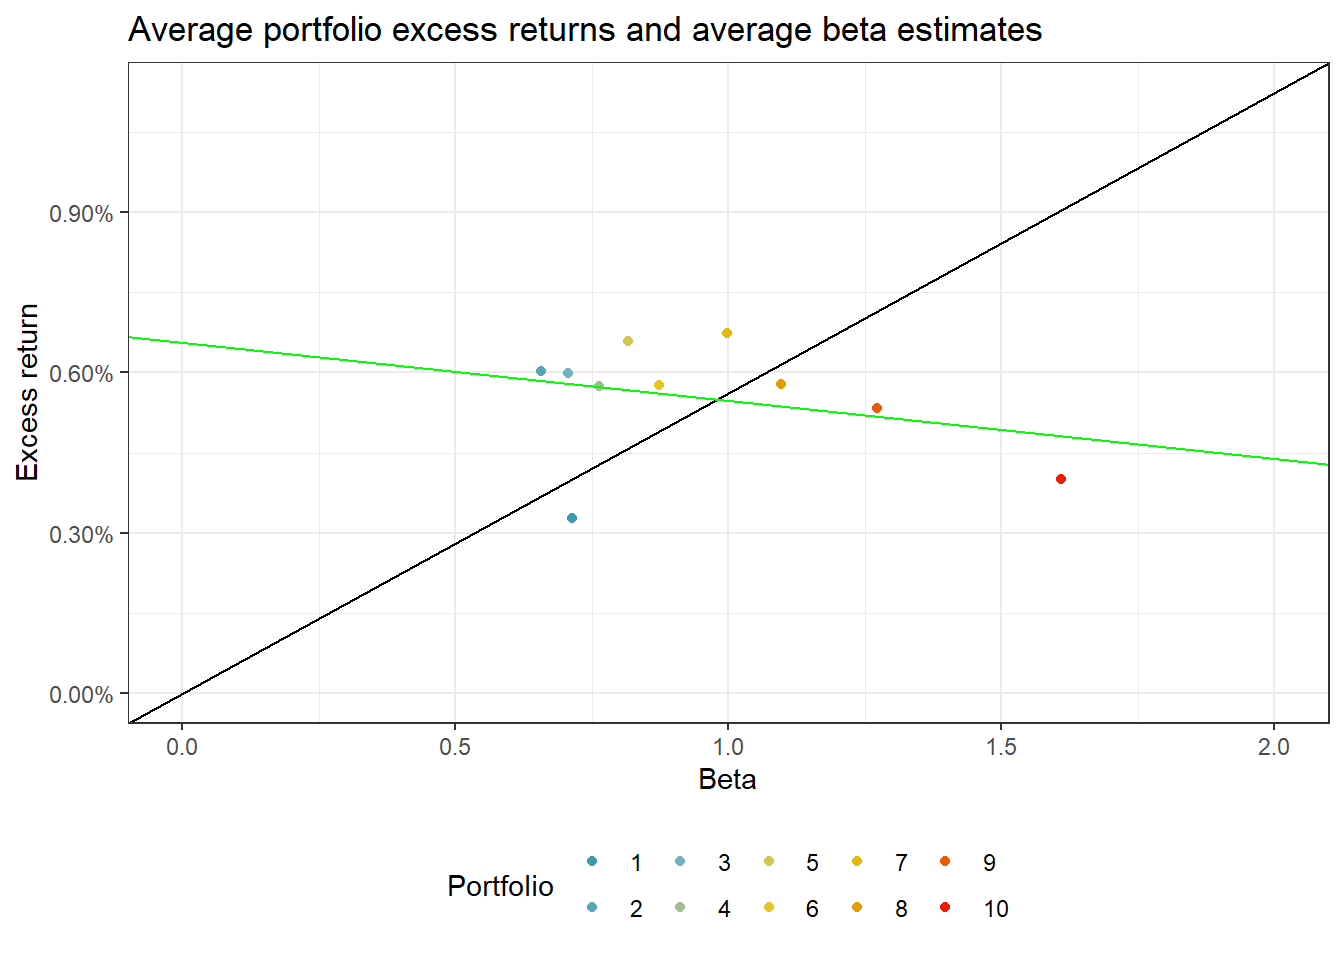
\includegraphics{32_univariate_sorts_files/figure-latex/unnamed-chunk-13-1} \end{center}

To provide more evidence against the CAPM predictions, we again form a long-short strategy that buys the high-beta portfolio and shorts the low-beta portfolio.

\begin{Shaded}
\begin{Highlighting}[]
\NormalTok{beta\_longshort }\OtherTok{\textless{}{-}}\NormalTok{ beta\_portfolios }\SpecialCharTok{|}\ErrorTok{\textgreater{}}
  \FunctionTok{ungroup}\NormalTok{() }\SpecialCharTok{|}\ErrorTok{\textgreater{}}
  \FunctionTok{mutate}\NormalTok{(}\AttributeTok{portfolio =} \FunctionTok{case\_when}\NormalTok{(}
\NormalTok{    portfolio }\SpecialCharTok{==} \FunctionTok{max}\NormalTok{(}\FunctionTok{as.numeric}\NormalTok{(portfolio)) }\SpecialCharTok{\textasciitilde{}} \StringTok{"high"}\NormalTok{,}
\NormalTok{    portfolio }\SpecialCharTok{==} \FunctionTok{min}\NormalTok{(}\FunctionTok{as.numeric}\NormalTok{(portfolio)) }\SpecialCharTok{\textasciitilde{}} \StringTok{"low"}
\NormalTok{  )) }\SpecialCharTok{|}\ErrorTok{\textgreater{}}
  \FunctionTok{filter}\NormalTok{(portfolio }\SpecialCharTok{\%in\%} \FunctionTok{c}\NormalTok{(}\StringTok{"low"}\NormalTok{, }\StringTok{"high"}\NormalTok{)) }\SpecialCharTok{|}\ErrorTok{\textgreater{}}
  \FunctionTok{pivot\_wider}\NormalTok{(month, }\AttributeTok{names\_from =}\NormalTok{ portfolio, }\AttributeTok{values\_from =}\NormalTok{ ret) }\SpecialCharTok{|}\ErrorTok{\textgreater{}}
  \FunctionTok{mutate}\NormalTok{(}\AttributeTok{long\_short =}\NormalTok{ high }\SpecialCharTok{{-}}\NormalTok{ low) }\SpecialCharTok{|}\ErrorTok{\textgreater{}}
  \FunctionTok{left\_join}\NormalTok{(factors\_ff\_monthly, }\AttributeTok{by =} \StringTok{"month"}\NormalTok{)}
\end{Highlighting}
\end{Shaded}

Again, the resulting long-short strategy does not exhibit statistically significant returns.

\begin{Shaded}
\begin{Highlighting}[]
\FunctionTok{coeftest}\NormalTok{(}\FunctionTok{lm}\NormalTok{(long\_short }\SpecialCharTok{\textasciitilde{}} \DecValTok{1}\NormalTok{, }\AttributeTok{data =}\NormalTok{ beta\_longshort), }
         \AttributeTok{vcov =}\NormalTok{ NeweyWest)}
\end{Highlighting}
\end{Shaded}

\begin{verbatim}
## 
## t test of coefficients:
## 
##             Estimate Std. Error t value Pr(>|t|)
## (Intercept) 0.000734   0.002483     0.3     0.77
\end{verbatim}

However, the long-short portfolio yields a statistically significant negative CAPM-adjusted alpha, although, controlling for the effect of beta, the average excess stock returns should be zero according to the CAPM. The results thus provide no evidence in support of the CAPM. The negative value has been documented as the so-called betting against beta factor (\citet{Frazzini2014}). Betting against beta corresponds to a strategy that shorts high beta stocks and takes a (levered) long position in low beta stocks. If borrowing constraints prevent investors from taking positions on the SML they are instead incentivized to buy high beta stocks, which leads to a relatively higher price (and therefore lower expected returns than implied by the CAPM) for such high beta stocks. As a result, the betting-against-beta strategy earns from providing liquidity to capital constraint investors with lower risk aversion.

\begin{Shaded}
\begin{Highlighting}[]
\FunctionTok{coeftest}\NormalTok{(}\FunctionTok{lm}\NormalTok{(long\_short }\SpecialCharTok{\textasciitilde{}} \DecValTok{1} \SpecialCharTok{+}\NormalTok{ mkt\_excess, }\AttributeTok{data =}\NormalTok{ beta\_longshort), }
         \AttributeTok{vcov =}\NormalTok{ NeweyWest)}
\end{Highlighting}
\end{Shaded}

\begin{verbatim}
## 
## t test of coefficients:
## 
##             Estimate Std. Error t value Pr(>|t|)    
## (Intercept) -0.00441    0.00262   -1.69    0.092 .  
## mkt_excess   0.89461    0.10214    8.76   <2e-16 ***
## ---
## Signif. codes:  
## 0 '***' 0.001 '**' 0.01 '*' 0.05 '.' 0.1 ' ' 1
\end{verbatim}

The plot below shows the annual returns of the extreme beta portfolios we are mainly interested in. The figure illustrates no consistent striking patterns over the last years - each portfolio exhibits periods with positive and negative annual returns.

\begin{Shaded}
\begin{Highlighting}[]
\NormalTok{beta\_longshort }\SpecialCharTok{|}\ErrorTok{\textgreater{}}
  \FunctionTok{group\_by}\NormalTok{(}\AttributeTok{year =} \FunctionTok{year}\NormalTok{(month)) }\SpecialCharTok{|}\ErrorTok{\textgreater{}}
  \FunctionTok{summarize}\NormalTok{(}
    \AttributeTok{low =} \FunctionTok{prod}\NormalTok{(}\DecValTok{1} \SpecialCharTok{+}\NormalTok{ low),}
    \AttributeTok{high =} \FunctionTok{prod}\NormalTok{(}\DecValTok{1} \SpecialCharTok{+}\NormalTok{ high),}
    \AttributeTok{long\_short =} \FunctionTok{prod}\NormalTok{(}\DecValTok{1} \SpecialCharTok{+}\NormalTok{ long\_short)}
\NormalTok{  ) }\SpecialCharTok{|}\ErrorTok{\textgreater{}}
  \FunctionTok{pivot\_longer}\NormalTok{(}\AttributeTok{cols =} \SpecialCharTok{{-}}\NormalTok{year) }\SpecialCharTok{|}\ErrorTok{\textgreater{}}
  \FunctionTok{ggplot}\NormalTok{(}\FunctionTok{aes}\NormalTok{(}\AttributeTok{x =}\NormalTok{ year, }\AttributeTok{y =} \DecValTok{1} \SpecialCharTok{{-}}\NormalTok{ value, }\AttributeTok{fill =}\NormalTok{ name)) }\SpecialCharTok{+}
  \FunctionTok{geom\_col}\NormalTok{(}\AttributeTok{position =} \StringTok{"dodge"}\NormalTok{) }\SpecialCharTok{+}
  \FunctionTok{facet\_wrap}\NormalTok{(}\SpecialCharTok{\textasciitilde{}}\NormalTok{name, }\AttributeTok{ncol =} \DecValTok{1}\NormalTok{) }\SpecialCharTok{+}
  \FunctionTok{theme}\NormalTok{(}\AttributeTok{legend.position =} \StringTok{"none"}\NormalTok{) }\SpecialCharTok{+}
  \FunctionTok{scale\_y\_continuous}\NormalTok{(}\AttributeTok{labels =}\NormalTok{ percent) }\SpecialCharTok{+}
  \FunctionTok{labs}\NormalTok{(}
    \AttributeTok{title =} \StringTok{"Annual returns of beta portfolios"}\NormalTok{,}
    \AttributeTok{x =} \ConstantTok{NULL}\NormalTok{, }\AttributeTok{y =} \ConstantTok{NULL}
\NormalTok{  )}
\end{Highlighting}
\end{Shaded}

\begin{center}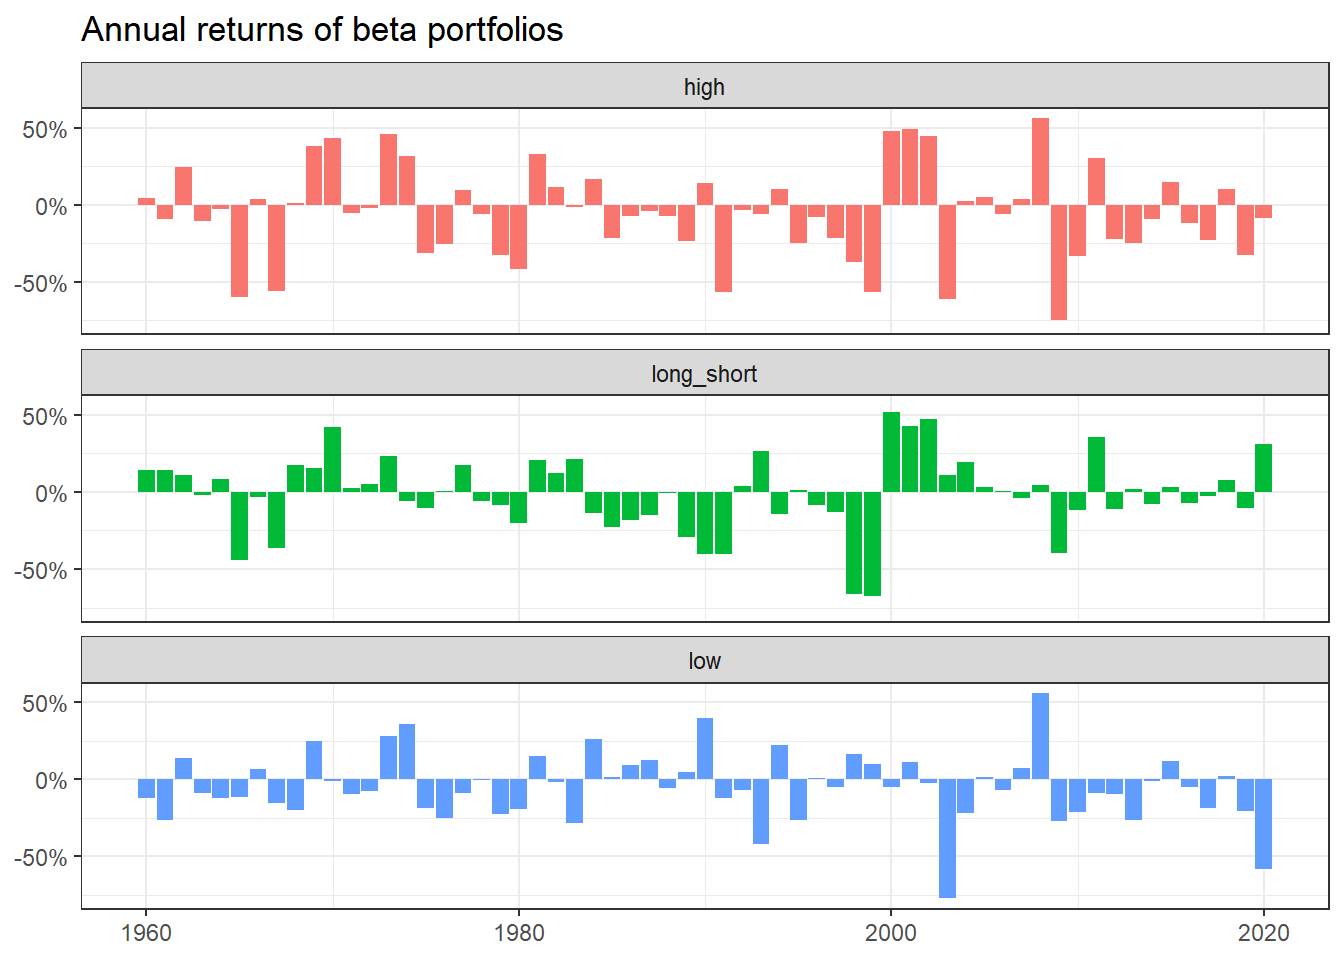
\includegraphics{32_univariate_sorts_files/figure-latex/unnamed-chunk-17-1} \end{center}

Overall, this chapter shows how functional programming can be leveraged to form an arbitrary number of portfolios using any sorting variable and how to evaluate the performance of the resulting portfolios. In the next chapter, we dive deeper into the many degrees of freedom that arise in the context of portfolio analysis.

\hypertarget{exercises-4}{%
\section{Exercises}\label{exercises-4}}

\begin{enumerate}
\def\labelenumi{\arabic{enumi}.}
\tightlist
\item
  Take the two long-short beta strategies based on different numbers of portfolios and compare the returns. Is there a significant difference in returns? How do the Sharpe ratios compare between the strategies? Find one additional portfolio evaluation statistic and compute it.
\item
  We plotted the alphas of the ten beta portfolios above. Write a function that tests these estimates for significance. Which portfolios have significant alphas?
\item
  The analysis here is based on betas from daily returns. However, we also computed betas from monthly returns. Re-run the analysis and point out differences in the results.
\item
  Given the results in this chapter, can you define a long-short strategy that yields positive abnormal returns (i.e., alphas)? Plot the cumulative excess return of your strategy and the market excess return for comparison.
\end{enumerate}

\hypertarget{size-sorts-and-p-hacking}{%
\chapter{Size sorts and p-hacking}\label{size-sorts-and-p-hacking}}

In this chapter, we continue with portfolio sorts in a univariate setting. Yet, we consider firm size as a sorting variable, which gives rise to a well-known return factor: the size premium. The size premium arises from buying small stocks and selling large stocks. Prominently, \citet{Fama1993} include it as a factor in their three-factor model. Apart from that, asset managers commonly include size as a key firm characteristic when making investment decisions.

We also introduce new choices in the formation of portfolios. In particular, we discuss listing exchanges, industries, weighting regimes, and periods. These choices matter for the portfolio returns and result in different size premiums. Exploiting these ideas to generate favorable results is called p-hacking.
There is arguably a thin line between p-hacking and conducting robustness tests, our purpose here is simply to illustrate the substantial variation which can arise along the evidence generating process.

\hypertarget{data-preparation-1}{%
\section{Data preparation}\label{data-preparation-1}}

The chapter relies on the following set of packages.

\begin{Shaded}
\begin{Highlighting}[]
\FunctionTok{library}\NormalTok{(tidyverse)}
\FunctionTok{library}\NormalTok{(RSQLite)}
\FunctionTok{library}\NormalTok{(lubridate)}
\FunctionTok{library}\NormalTok{(sandwich)}
\FunctionTok{library}\NormalTok{(lmtest)}
\FunctionTok{library}\NormalTok{(scales)}
\FunctionTok{library}\NormalTok{(furrr)}
\end{Highlighting}
\end{Shaded}

First, we retrieve the relevant data from our \texttt{SQLite}-database introduced in our chapter on \emph{``Accessing \& managing financial data''}. Firm size is defined as market equity in most asset pricing applications that we retrieve from CRSP. We further use the Fama-French factor returns for performance evaluation.

\begin{Shaded}
\begin{Highlighting}[]
\NormalTok{tidy\_finance }\OtherTok{\textless{}{-}} \FunctionTok{dbConnect}\NormalTok{(}
  \FunctionTok{SQLite}\NormalTok{(), }\StringTok{"data/tidy\_finance.sqlite"}\NormalTok{, }\AttributeTok{extended\_types =} \ConstantTok{TRUE}
\NormalTok{)}

\NormalTok{crsp\_monthly }\OtherTok{\textless{}{-}} \FunctionTok{tbl}\NormalTok{(tidy\_finance, }\StringTok{"crsp\_monthly"}\NormalTok{) }\SpecialCharTok{|}\ErrorTok{\textgreater{}}
  \FunctionTok{collect}\NormalTok{()}

\NormalTok{factors\_ff\_monthly }\OtherTok{\textless{}{-}} \FunctionTok{tbl}\NormalTok{(tidy\_finance, }\StringTok{"factors\_ff\_monthly"}\NormalTok{) }\SpecialCharTok{|}\ErrorTok{\textgreater{}}
  \FunctionTok{collect}\NormalTok{()}
\end{Highlighting}
\end{Shaded}

\hypertarget{size-distribution}{%
\section{Size distribution}\label{size-distribution}}

Before we build our size portfolios, we investigate the distribution of the variable \emph{firm size}. Visualizing the data is a valuable starting point to understand the input to the analysis. The figure below shows the fraction of total market capitalization concentrated in the largest firm. To produce this graph, we create monthly indicators that track whether a stock belongs to the largest x\% of the firms.
Then, we aggregate the firms within each bucket and compute the buckets' share of total market capitalization.

The figure shows that the largest 1\% of firms cover up to 50\% of the total market capitalization, and holding just the 25\% largest firms in the CRSP universe essentially replicates the market portfolio. The distribution of firm size thus implies that the largest firms of the market dominate many small firms whenever we use value-weighted benchmarks.

\begin{Shaded}
\begin{Highlighting}[]
\NormalTok{crsp\_monthly }\SpecialCharTok{|}\ErrorTok{\textgreater{}}
  \FunctionTok{group\_by}\NormalTok{(month) }\SpecialCharTok{|}\ErrorTok{\textgreater{}}
  \FunctionTok{mutate}\NormalTok{(}
    \AttributeTok{top01 =} \FunctionTok{if\_else}\NormalTok{(mktcap }\SpecialCharTok{\textgreater{}=} \FunctionTok{quantile}\NormalTok{(mktcap, }\FloatTok{0.99}\NormalTok{), 1L, 0L),}
    \AttributeTok{top05 =} \FunctionTok{if\_else}\NormalTok{(mktcap }\SpecialCharTok{\textgreater{}=} \FunctionTok{quantile}\NormalTok{(mktcap, }\FloatTok{0.95}\NormalTok{), 1L, 0L),}
    \AttributeTok{top10 =} \FunctionTok{if\_else}\NormalTok{(mktcap }\SpecialCharTok{\textgreater{}=} \FunctionTok{quantile}\NormalTok{(mktcap, }\FloatTok{0.90}\NormalTok{), 1L, 0L),}
    \AttributeTok{top25 =} \FunctionTok{if\_else}\NormalTok{(mktcap }\SpecialCharTok{\textgreater{}=} \FunctionTok{quantile}\NormalTok{(mktcap, }\FloatTok{0.75}\NormalTok{), 1L, 0L),}
    \AttributeTok{total\_market\_cap =} \FunctionTok{sum}\NormalTok{(mktcap)}
\NormalTok{  ) }\SpecialCharTok{|}\ErrorTok{\textgreater{}}
  \FunctionTok{summarize}\NormalTok{(}
    \StringTok{\textasciigrave{}}\AttributeTok{Largest 1\% of stocks}\StringTok{\textasciigrave{}} \OtherTok{=} \FunctionTok{sum}\NormalTok{(mktcap[top01 }\SpecialCharTok{==} \DecValTok{1}\NormalTok{]) }\SpecialCharTok{/}\NormalTok{ total\_market\_cap,}
    \StringTok{\textasciigrave{}}\AttributeTok{Largest 5\% of stocks}\StringTok{\textasciigrave{}} \OtherTok{=} \FunctionTok{sum}\NormalTok{(mktcap[top05 }\SpecialCharTok{==} \DecValTok{1}\NormalTok{]) }\SpecialCharTok{/}\NormalTok{ total\_market\_cap,}
    \StringTok{\textasciigrave{}}\AttributeTok{Largest 10\% of stocks}\StringTok{\textasciigrave{}} \OtherTok{=} \FunctionTok{sum}\NormalTok{(mktcap[top10 }\SpecialCharTok{==} \DecValTok{1}\NormalTok{]) }\SpecialCharTok{/}\NormalTok{ total\_market\_cap,}
    \StringTok{\textasciigrave{}}\AttributeTok{Largest 25\% of stocks}\StringTok{\textasciigrave{}} \OtherTok{=} \FunctionTok{sum}\NormalTok{(mktcap[top25 }\SpecialCharTok{==} \DecValTok{1}\NormalTok{]) }\SpecialCharTok{/}\NormalTok{ total\_market\_cap}
\NormalTok{  ) }\SpecialCharTok{|}\ErrorTok{\textgreater{}}
  \FunctionTok{pivot\_longer}\NormalTok{(}\AttributeTok{cols =} \SpecialCharTok{{-}}\NormalTok{month) }\SpecialCharTok{|}\ErrorTok{\textgreater{}}
  \FunctionTok{mutate}\NormalTok{(}\AttributeTok{name =} \FunctionTok{factor}\NormalTok{(name, }\AttributeTok{levels =} \FunctionTok{c}\NormalTok{(}
    \StringTok{"Largest 1\% of stocks"}\NormalTok{, }\StringTok{"Largest 5\% of stocks"}\NormalTok{,}
    \StringTok{"Largest 10\% of stocks"}\NormalTok{, }\StringTok{"Largest 25\% of stocks"}
\NormalTok{  ))) }\SpecialCharTok{|}\ErrorTok{\textgreater{}}
  \FunctionTok{ggplot}\NormalTok{(}\FunctionTok{aes}\NormalTok{(}\AttributeTok{x =}\NormalTok{ month, }\AttributeTok{y =}\NormalTok{ value, }\AttributeTok{color =}\NormalTok{ name)) }\SpecialCharTok{+}
  \FunctionTok{geom\_line}\NormalTok{() }\SpecialCharTok{+}
  \FunctionTok{scale\_y\_continuous}\NormalTok{(}\AttributeTok{labels =}\NormalTok{ percent, }\AttributeTok{limits =} \FunctionTok{c}\NormalTok{(}\DecValTok{0}\NormalTok{, }\DecValTok{1}\NormalTok{)) }\SpecialCharTok{+}
  \FunctionTok{labs}\NormalTok{(}
    \AttributeTok{x =} \ConstantTok{NULL}\NormalTok{, }\AttributeTok{y =} \ConstantTok{NULL}\NormalTok{, }\AttributeTok{color =} \ConstantTok{NULL}\NormalTok{,}
    \AttributeTok{title =} \StringTok{"Percentage of total market capitalization in largest stocks"}
\NormalTok{  )}
\end{Highlighting}
\end{Shaded}

\begin{center}\includegraphics{33_size_and_portfolio_building_files/figure-latex/unnamed-chunk-3-1} \end{center}

Next, firm sizes also differ across listing exchanges. Stocks' primary listings were important in the past and are potentially still relevant today. The graph below shows that the New York Stock Exchange (NYSE) was and still is the largest listing exchange in terms of market capitalization. More recently, NASDAQ has gained relevance as a listing exchange. Do you know what the small peak in NASDAQ's market cap around the year 2000 was?

\begin{Shaded}
\begin{Highlighting}[]
\NormalTok{crsp\_monthly }\SpecialCharTok{|}\ErrorTok{\textgreater{}}
  \FunctionTok{group\_by}\NormalTok{(month, exchange) }\SpecialCharTok{|}\ErrorTok{\textgreater{}}
  \FunctionTok{summarize}\NormalTok{(}\AttributeTok{mktcap =} \FunctionTok{sum}\NormalTok{(mktcap)) }\SpecialCharTok{|}\ErrorTok{\textgreater{}}
  \FunctionTok{mutate}\NormalTok{(}\AttributeTok{share =}\NormalTok{ mktcap }\SpecialCharTok{/} \FunctionTok{sum}\NormalTok{(mktcap)) }\SpecialCharTok{|}\ErrorTok{\textgreater{}}
  \FunctionTok{ggplot}\NormalTok{(}\FunctionTok{aes}\NormalTok{(}\AttributeTok{x =}\NormalTok{ month, }\AttributeTok{y =}\NormalTok{ share, }\AttributeTok{fill =}\NormalTok{ exchange, }\AttributeTok{color =}\NormalTok{ exchange)) }\SpecialCharTok{+}
  \FunctionTok{geom\_area}\NormalTok{(}
    \AttributeTok{position =} \StringTok{"stack"}\NormalTok{,}
    \AttributeTok{stat =} \StringTok{"identity"}\NormalTok{,}
    \AttributeTok{alpha =} \FloatTok{0.5}
\NormalTok{  ) }\SpecialCharTok{+}
  \FunctionTok{geom\_line}\NormalTok{(}\AttributeTok{position =} \StringTok{"stack"}\NormalTok{) }\SpecialCharTok{+}
  \FunctionTok{scale\_y\_continuous}\NormalTok{(}\AttributeTok{labels =}\NormalTok{ percent) }\SpecialCharTok{+}
  \FunctionTok{labs}\NormalTok{(}
    \AttributeTok{x =} \ConstantTok{NULL}\NormalTok{, }\AttributeTok{y =} \ConstantTok{NULL}\NormalTok{, }\AttributeTok{fill =} \ConstantTok{NULL}\NormalTok{, }\AttributeTok{color =} \ConstantTok{NULL}\NormalTok{,}
    \AttributeTok{title =} \StringTok{"Share of total market capitalization per listing exchange"}
\NormalTok{  )}
\end{Highlighting}
\end{Shaded}

\begin{center}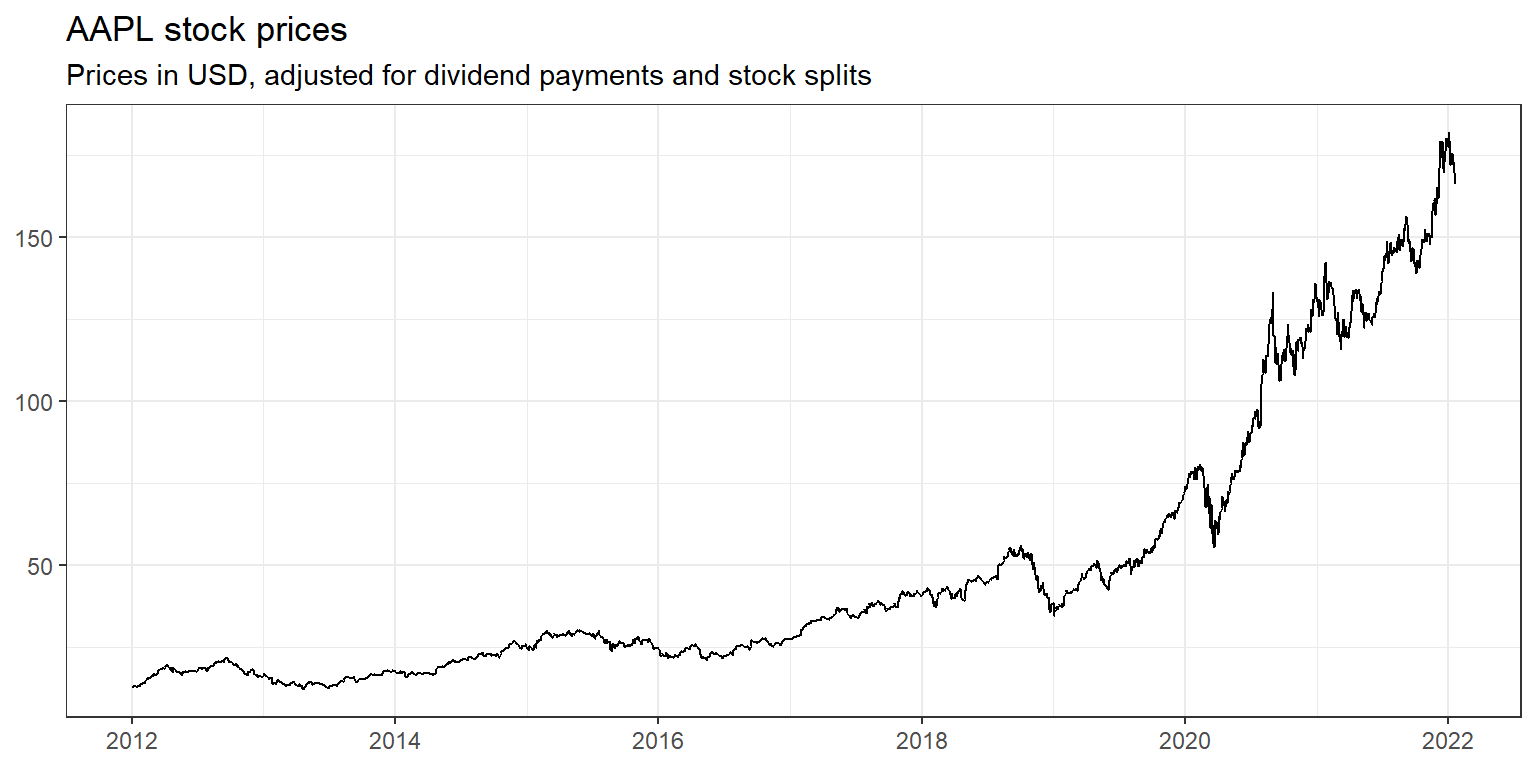
\includegraphics{33_size_and_portfolio_building_files/figure-latex/unnamed-chunk-4-1} \end{center}

Finally, we consider the distribution of firm size across listing exchanges and create summary statistics. The function \texttt{base::summary()} does not include all statistics we are interested in, which is why we create the function \texttt{create\_summary()} that adds the standard deviation and the number of observations. Then, we apply it to the most current month of our CRSP data on each listing exchange. We also add a row with \texttt{tibble::add\_row()} with the overall summary statistics.

The resulting table shows that firms listed on NYSE are significantly larger on average than firms listed on the other exchanges. Moreover, NASDAQ lists the largest number of firms. This discrepancy between firm sizes across listing exchanges motivated researchers to form breakpoints exclusively on the NYSE sample and apply those breakpoints to all stocks. In the following, we use this distinction to update our portfolio sort procedure.

\begin{Shaded}
\begin{Highlighting}[]
\NormalTok{create\_summary }\OtherTok{\textless{}{-}} \ControlFlowTok{function}\NormalTok{(data, column\_name) \{}
\NormalTok{  data }\SpecialCharTok{|}\ErrorTok{\textgreater{}}
    \FunctionTok{select}\NormalTok{(}\AttributeTok{value =}\NormalTok{ \{\{ column\_name \}\}) }\SpecialCharTok{|}\ErrorTok{\textgreater{}}
    \FunctionTok{summarize}\NormalTok{(}
      \AttributeTok{mean =} \FunctionTok{mean}\NormalTok{(value),}
      \AttributeTok{sd =} \FunctionTok{sd}\NormalTok{(value),}
      \AttributeTok{min =} \FunctionTok{min}\NormalTok{(value),}
      \AttributeTok{q05 =} \FunctionTok{quantile}\NormalTok{(value, }\FloatTok{0.05}\NormalTok{),}
      \AttributeTok{q25 =} \FunctionTok{quantile}\NormalTok{(value, }\FloatTok{0.25}\NormalTok{),}
      \AttributeTok{q50 =} \FunctionTok{quantile}\NormalTok{(value, }\FloatTok{0.50}\NormalTok{),}
      \AttributeTok{q75 =} \FunctionTok{quantile}\NormalTok{(value, }\FloatTok{0.75}\NormalTok{),}
      \AttributeTok{q95 =} \FunctionTok{quantile}\NormalTok{(value, }\FloatTok{0.95}\NormalTok{),}
      \AttributeTok{max =} \FunctionTok{max}\NormalTok{(value),}
      \AttributeTok{n =} \FunctionTok{n}\NormalTok{()}
\NormalTok{    )}
\NormalTok{\}}

\NormalTok{crsp\_monthly }\SpecialCharTok{|}\ErrorTok{\textgreater{}}
  \FunctionTok{filter}\NormalTok{(month }\SpecialCharTok{==} \FunctionTok{max}\NormalTok{(month)) }\SpecialCharTok{|}\ErrorTok{\textgreater{}}
  \FunctionTok{group\_by}\NormalTok{(exchange) }\SpecialCharTok{|}\ErrorTok{\textgreater{}}
  \FunctionTok{create\_summary}\NormalTok{(mktcap) }\SpecialCharTok{|}\ErrorTok{\textgreater{}}
  \FunctionTok{add\_row}\NormalTok{(crsp\_monthly }\SpecialCharTok{|}\ErrorTok{\textgreater{}}
    \FunctionTok{filter}\NormalTok{(month }\SpecialCharTok{==} \FunctionTok{max}\NormalTok{(month)) }\SpecialCharTok{|}\ErrorTok{\textgreater{}}
    \FunctionTok{create\_summary}\NormalTok{(mktcap) }\SpecialCharTok{|}\ErrorTok{\textgreater{}}
    \FunctionTok{mutate}\NormalTok{(}\AttributeTok{exchange =} \StringTok{"Overall"}\NormalTok{))}
\end{Highlighting}
\end{Shaded}

\begin{verbatim}
## # A tibble: 5 x 11
##   exchange   mean     sd      min     q05    q25    q50
##   <chr>     <dbl>  <dbl>    <dbl>   <dbl>  <dbl>  <dbl>
## 1 AMEX       283.  1298.     6.04    10.1 3.07e1 6.59e1
## 2 NASDAQ    8041. 74386.     4.65    27.3 1.34e2 4.85e2
## 3 NYSE     16427. 43130.     5.35   154.  9.16e2 3.34e3
## 4 Other    10061.    NA  10061.   10061.  1.01e4 1.01e4
## 5 Overall  10558. 63975.     4.65    31.0 1.85e2 8.72e2
## # ... with 4 more variables: q75 <dbl>, q95 <dbl>,
## #   max <dbl>, n <int>
\end{verbatim}

\hypertarget{univariate-size-portfolios-with-flexible-breakpoints}{%
\section{Univariate size portfolios with flexible breakpoints}\label{univariate-size-portfolios-with-flexible-breakpoints}}

In the previous chapter, we construct portfolios with a varying number of portfolios and different sorting variables. Here, we extend the framework such that we compute breakpoints on a subset of the data, for instance, based on selected listing exchanges. In published asset pricing articles, many scholars compute sorting breakpoints only on NYSE-listed stocks. These NYSE-specific breakpoints are then applied to the entire universe of stocks.

To replicate the NYSE-centered sorting procedure, we introduce \texttt{exchanges} as an argument in our \texttt{assign\_portfolio()} function. The exchange-specific argument then enters in the filter \texttt{filter(grepl(exchanges,\ exchange))}. The function \texttt{base::grepl()} is part of a family of functions on \emph{regular expressions}, which provide various functionalities to work and manipulate character strings. Here, we replace the character string stored in the column \texttt{exchange} with a binary variable that indicates if the string matches the pattern specified in the argument \texttt{exchanges}. For example, if \texttt{exchanges\ =\ \textquotesingle{}NYSE\textquotesingle{}} is specified, only stocks from NYSE are used to compute the breakpoints. Alternatively, you could specify \texttt{exchanges\ =\ \textquotesingle{}NYSE\textbar{}NASDAQ\textbar{}AMEX\textquotesingle{}}, which keeps all stocks listed on either of these exchanges. Overall, regular expressions are a powerful tool, and we only touch on a specific case here.

\begin{Shaded}
\begin{Highlighting}[]
\NormalTok{assign\_portfolio }\OtherTok{\textless{}{-}} \ControlFlowTok{function}\NormalTok{(n\_portfolios,}
\NormalTok{                             exchanges,}
\NormalTok{                             data) \{}
\NormalTok{  breakpoints }\OtherTok{\textless{}{-}}\NormalTok{ data }\SpecialCharTok{|}\ErrorTok{\textgreater{}}
    \FunctionTok{filter}\NormalTok{(}\FunctionTok{grepl}\NormalTok{(exchanges, exchange)) }\SpecialCharTok{|}\ErrorTok{\textgreater{}}
    \FunctionTok{summarize}\NormalTok{(}\AttributeTok{breakpoint =} \FunctionTok{quantile}\NormalTok{(}
\NormalTok{      mktcap\_lag,}
      \AttributeTok{probs =} \FunctionTok{seq}\NormalTok{(}\DecValTok{0}\NormalTok{, }\DecValTok{1}\NormalTok{, }\AttributeTok{length.out =}\NormalTok{ n\_portfolios }\SpecialCharTok{+} \DecValTok{1}\NormalTok{),}
      \AttributeTok{na.rm =} \ConstantTok{TRUE}
\NormalTok{    )) }\SpecialCharTok{|}\ErrorTok{\textgreater{}}
    \FunctionTok{pull}\NormalTok{(breakpoint) }\SpecialCharTok{|}\ErrorTok{\textgreater{}}
    \FunctionTok{as.numeric}\NormalTok{()}

\NormalTok{  data }\SpecialCharTok{|}\ErrorTok{\textgreater{}}
    \FunctionTok{mutate}\NormalTok{(}\AttributeTok{portfolio =} \FunctionTok{findInterval}\NormalTok{(mktcap\_lag, }
\NormalTok{                                    breakpoints, }\AttributeTok{all.inside =} \ConstantTok{TRUE}\NormalTok{)) }\SpecialCharTok{|}\ErrorTok{\textgreater{}}
    \FunctionTok{pull}\NormalTok{(portfolio)}
\NormalTok{\}}
\end{Highlighting}
\end{Shaded}

\hypertarget{weighting-schemes-for-portfolios}{%
\section{Weighting schemes for portfolios}\label{weighting-schemes-for-portfolios}}

Apart from computing breakpoints on different samples, researchers often use different portfolio weighting schemes. So far, we weighted each portfolio constituent by its relative market equity of the previous period. This protocol is called \emph{value-weighting}. The alternative protocol is \emph{equal-weighting}, which assigns each stock's return the same weight, i.e., a simple average of the constituents' returns. Notice that equal-weighting is difficult in practice as the portfolio manager needs to rebalance the portfolio monthly while value-weighting is a truly passive investment.

We implement the two weighting schemes in the function \texttt{compute\_portfolio\_returns()} that takes a logical argument to weight the returns by firm value. The statement \texttt{if\_else(value\_weighted,\ weighted.mean(ret\_excess,\ mktcap\_lag),\ mean(ret\_excess))} generates value-weighted returns if \texttt{value\_weighted\ =\ TRUE}. Additionally, the long-short portfolio is long in the smallest firms and short in the largest firms, consistent with research showing that small firms outperform their larger counterparts. Apart from these two changes, the function is similar to the procedure in the previous chapter.

\begin{Shaded}
\begin{Highlighting}[]
\NormalTok{compute\_portfolio\_returns }\OtherTok{\textless{}{-}} \ControlFlowTok{function}\NormalTok{(}\AttributeTok{n\_portfolios =} \DecValTok{10}\NormalTok{,}
                                      \AttributeTok{exchanges =} \StringTok{"NYSE|NASDAQ|AMEX"}\NormalTok{,}
                                      \AttributeTok{value\_weighted =} \ConstantTok{TRUE}\NormalTok{,}
                                      \AttributeTok{data =}\NormalTok{ crsp\_monthly) \{}
\NormalTok{  data }\SpecialCharTok{|}\ErrorTok{\textgreater{}}
    \FunctionTok{group\_by}\NormalTok{(month) }\SpecialCharTok{|}\ErrorTok{\textgreater{}}
    \FunctionTok{mutate}\NormalTok{(}\AttributeTok{portfolio =} \FunctionTok{assign\_portfolio}\NormalTok{(}
      \AttributeTok{n\_portfolios =}\NormalTok{ n\_portfolios,}
      \AttributeTok{exchanges =}\NormalTok{ exchanges,}
      \AttributeTok{data =} \FunctionTok{cur\_data}\NormalTok{()}
\NormalTok{    )) }\SpecialCharTok{|}\ErrorTok{\textgreater{}}
    \FunctionTok{group\_by}\NormalTok{(month, portfolio) }\SpecialCharTok{|}\ErrorTok{\textgreater{}}
    \FunctionTok{summarize}\NormalTok{(}
      \AttributeTok{ret =} \FunctionTok{if\_else}\NormalTok{(value\_weighted, }
                    \FunctionTok{weighted.mean}\NormalTok{(ret\_excess, mktcap\_lag), }\FunctionTok{mean}\NormalTok{(ret\_excess)),}
      \AttributeTok{.groups =} \StringTok{"drop\_last"}
\NormalTok{    ) }\SpecialCharTok{|}\ErrorTok{\textgreater{}}
    \FunctionTok{summarize}\NormalTok{(}\AttributeTok{size\_premium =}\NormalTok{ ret[portfolio }\SpecialCharTok{==} \FunctionTok{min}\NormalTok{(portfolio)] }\SpecialCharTok{{-}} 
\NormalTok{                ret[portfolio }\SpecialCharTok{==} \FunctionTok{max}\NormalTok{(portfolio)]) }\SpecialCharTok{|}\ErrorTok{\textgreater{}}
    \FunctionTok{summarize}\NormalTok{(}\AttributeTok{size\_premium =} \FunctionTok{mean}\NormalTok{(size\_premium))}
\NormalTok{\}}
\end{Highlighting}
\end{Shaded}

To see how the function \texttt{compute\_portfolio\_returns()} works, we consider a simple median breakpoint example with value-weighted returns. We are interested in the effect of restricting listing exchanges on the estimation of the size premium. In the first function call, we compute returns based on breakpoints from all listing exchanges. Then, we computed returns based on breakpoints from NYSE-listed stocks.

\begin{Shaded}
\begin{Highlighting}[]
\NormalTok{ret\_all }\OtherTok{\textless{}{-}} \FunctionTok{compute\_portfolio\_returns}\NormalTok{(}
  \AttributeTok{n\_portfolios =} \DecValTok{2}\NormalTok{,}
  \AttributeTok{exchanges =} \StringTok{"NYSE|NASDAQ|AMEX"}\NormalTok{,}
  \AttributeTok{value\_weighted =} \ConstantTok{TRUE}\NormalTok{,}
  \AttributeTok{data =}\NormalTok{ crsp\_monthly}
\NormalTok{)}

\NormalTok{ret\_nyse }\OtherTok{\textless{}{-}} \FunctionTok{compute\_portfolio\_returns}\NormalTok{(}
  \AttributeTok{n\_portfolios =} \DecValTok{2}\NormalTok{,}
  \AttributeTok{exchanges =} \StringTok{"NYSE"}\NormalTok{,}
  \AttributeTok{value\_weighted =} \ConstantTok{TRUE}\NormalTok{,}
  \AttributeTok{data =}\NormalTok{ crsp\_monthly}
\NormalTok{)}

\FunctionTok{tibble}\NormalTok{(}\AttributeTok{Exchanges =} \FunctionTok{c}\NormalTok{(}\StringTok{"all"}\NormalTok{, }\StringTok{"NYSE"}\NormalTok{), }
       \AttributeTok{Premium =} \FunctionTok{as.numeric}\NormalTok{(}\FunctionTok{c}\NormalTok{(ret\_all, ret\_nyse)) }\SpecialCharTok{*} \DecValTok{100}\NormalTok{)}
\end{Highlighting}
\end{Shaded}

\begin{verbatim}
## # A tibble: 2 x 2
##   Exchanges Premium
##   <chr>       <dbl>
## 1 all         0.110
## 2 NYSE        0.181
\end{verbatim}

The table shows that the size premium is more than 60\% larger if we consider only stocks from NYSE to form the breakpoint each month. The NYSE-specific breakpoints are larger, and there are more than 50\% of the stocks in the entire universe in the resulting small portfolio because NYSE firms are larger on average. The impact of this choice is not negligible.

\hypertarget{p-hacking-and-non-standard-errors}{%
\section{P-hacking and non-standard errors}\label{p-hacking-and-non-standard-errors}}

Since the choice of the exchange has a significant impact, the next step is to investigate the effect of other data processing decisions researchers have to make along the way. In particular, any portfolio sort analysis has to decide at least on the number of portfolios, the listing exchanges to form breakpoints, and equal- or value-weighting. Further, one may exclude firms that are active in the finance industry or restrict the analysis to some parts of the time series. All of the variations of these choices that we discuss here are part of scholarly articles published in the top finance journals.
The intention of this application is to show that the different ways to form portfolios result in different estimated size premia. Despite the effects of this multitude of choices, there is no correct way. It should also be noted that none of the procedures is wrong, the aim is simply to illustrate the changes that can arise due to the variation in the evidence-generating process \citep{Menkveld2022}.
From a malicious perspective, these modeling choices give the researcher multiple \emph{chances} to find statistically significant results. Yet this is considered \emph{p-hacking} which renders the statistical inference due to multiple testing invalid \citep{Harvey2016}.

Nevertheless, the multitude of options creates a problem since there is no single correct way of sorting portfolios. How should a researcher convince a reader that their results do not come from a p-hacking exercise? To circumvent this dilemma, academics are encouraged to present evidence from different sorting schemes as \emph{robustness tests} and report multiple approaches to show that a result does not depend on a single choice. Thus, the robustness of premiums is a key feature.

Below we conduct a series of robustness tests which could also be interpreted as a p-hacking exercise. To do so, we examine the size premium in different specifications presented in the table \texttt{p\_hacking\_setup}. The function \texttt{tidyr::expand\_grid()} produces a table of all possible permutations of its arguments. Notice that we use the argument \texttt{data} to exclude financial firms and truncate the time series.

\begin{Shaded}
\begin{Highlighting}[]
\NormalTok{p\_hacking\_setup }\OtherTok{\textless{}{-}} \FunctionTok{expand\_grid}\NormalTok{(}
  \AttributeTok{n\_portfolios =} \FunctionTok{c}\NormalTok{(}\DecValTok{2}\NormalTok{, }\DecValTok{5}\NormalTok{, }\DecValTok{10}\NormalTok{),}
  \AttributeTok{exchanges =} \FunctionTok{c}\NormalTok{(}\StringTok{"NYSE"}\NormalTok{, }\StringTok{"NYSE|NASDAQ|AMEX"}\NormalTok{),}
  \AttributeTok{value\_weighted =} \FunctionTok{c}\NormalTok{(}\ConstantTok{TRUE}\NormalTok{, }\ConstantTok{FALSE}\NormalTok{),}
  \AttributeTok{data =}\NormalTok{ rlang}\SpecialCharTok{::}\FunctionTok{parse\_exprs}\NormalTok{(}
  \StringTok{\textquotesingle{}crsp\_monthly; crsp\_monthly |\textgreater{} filter(industry != "Finance");}
\StringTok{   crsp\_monthly |\textgreater{} filter(month \textless{} "1990{-}06{-}01");}
\StringTok{   crsp\_monthly |\textgreater{} filter(month \textgreater{}="1990{-}06{-}01")\textquotesingle{}}\NormalTok{)}
\NormalTok{)}
\NormalTok{p\_hacking\_setup}
\end{Highlighting}
\end{Shaded}

\begin{verbatim}
## # A tibble: 48 x 4
##   n_portfolios exchanges value_weighted data      
##          <dbl> <chr>     <lgl>          <list>    
## 1            2 NYSE      TRUE           <sym>     
## 2            2 NYSE      TRUE           <language>
## 3            2 NYSE      TRUE           <language>
## 4            2 NYSE      TRUE           <language>
## 5            2 NYSE      FALSE          <sym>     
## # ... with 43 more rows
\end{verbatim}

To speed the computation up we parallelize the (many) different sorting procedures, as in Chapter 3. Finally, we report the resulting size premiums in descending order. There are indeed substantial size premia possible in our data, in particular when we use equal-weighted portfolios.

\begin{Shaded}
\begin{Highlighting}[]
\FunctionTok{plan}\NormalTok{(multisession, }\AttributeTok{workers =} \FunctionTok{availableCores}\NormalTok{())}

\NormalTok{p\_hacking\_setup }\OtherTok{\textless{}{-}}\NormalTok{ p\_hacking\_setup }\SpecialCharTok{|}\ErrorTok{\textgreater{}}
  \FunctionTok{mutate}\NormalTok{(}\AttributeTok{size\_premium =} \FunctionTok{future\_pmap}\NormalTok{(}
    \AttributeTok{.l =} \FunctionTok{list}\NormalTok{(}
\NormalTok{      n\_portfolios,}
\NormalTok{      exchanges,}
\NormalTok{      value\_weighted,}
\NormalTok{      data}
\NormalTok{    ),}
    \AttributeTok{.f =} \SpecialCharTok{\textasciitilde{}} \FunctionTok{compute\_portfolio\_returns}\NormalTok{(}
      \AttributeTok{n\_portfolios =}\NormalTok{ ..}\DecValTok{1}\NormalTok{,}
      \AttributeTok{exchanges =}\NormalTok{ ..}\DecValTok{2}\NormalTok{,}
      \AttributeTok{value\_weighted =}\NormalTok{ ..}\DecValTok{3}\NormalTok{,}
      \AttributeTok{data =}\NormalTok{ rlang}\SpecialCharTok{::}\FunctionTok{eval\_tidy}\NormalTok{(..}\DecValTok{4}\NormalTok{)}
\NormalTok{    )}
\NormalTok{  ))}

\NormalTok{p\_hacking\_results }\OtherTok{\textless{}{-}}\NormalTok{ p\_hacking\_setup }\SpecialCharTok{|}\ErrorTok{\textgreater{}}
  \FunctionTok{mutate}\NormalTok{(}\AttributeTok{data =} \FunctionTok{map\_chr}\NormalTok{(data, deparse)) }\SpecialCharTok{|}\ErrorTok{\textgreater{}}
  \FunctionTok{unnest}\NormalTok{(size\_premium) }\SpecialCharTok{|}\ErrorTok{\textgreater{}}
  \FunctionTok{mutate}\NormalTok{(}\AttributeTok{data =} \FunctionTok{str\_remove}\NormalTok{(data, }\StringTok{"crsp\_monthly |\textgreater{} "}\NormalTok{)) }\SpecialCharTok{|}\ErrorTok{\textgreater{}}
  \FunctionTok{arrange}\NormalTok{(}\FunctionTok{desc}\NormalTok{(size\_premium))}
\NormalTok{p\_hacking\_results}
\end{Highlighting}
\end{Shaded}

\begin{verbatim}
## # A tibble: 48 x 5
##   n_portfolios exchanges        value_weighted data    
##          <dbl> <chr>            <lgl>          <chr>   
## 1           10 NYSE|NASDAQ|AMEX FALSE          "filter~
## 2           10 NYSE|NASDAQ|AMEX FALSE          "filter~
## 3           10 NYSE|NASDAQ|AMEX FALSE          "crsp_m~
## 4           10 NYSE|NASDAQ|AMEX FALSE          "filter~
## 5           10 NYSE|NASDAQ|AMEX TRUE           "filter~
## # ... with 43 more rows, and 1 more variable:
## #   size_premium <dbl>
\end{verbatim}

\hypertarget{the-size-premium-variation}{%
\section{The size-premium variation}\label{the-size-premium-variation}}

We provide a graph that shows the different premiums. This plot also shows the relation to the average Fama-French SMB (small minus big) premium used in the literature which we include as a dotted vertical line.

\begin{Shaded}
\begin{Highlighting}[]
\NormalTok{p\_hacking\_results }\SpecialCharTok{|}\ErrorTok{\textgreater{}}
  \FunctionTok{ggplot}\NormalTok{(}\FunctionTok{aes}\NormalTok{(}\AttributeTok{x =}\NormalTok{ size\_premium)) }\SpecialCharTok{+}
  \FunctionTok{geom\_histogram}\NormalTok{(}\AttributeTok{bins =} \FunctionTok{nrow}\NormalTok{(p\_hacking\_results)) }\SpecialCharTok{+}
  \FunctionTok{labs}\NormalTok{(}
    \AttributeTok{x =} \ConstantTok{NULL}\NormalTok{, }\AttributeTok{y =} \ConstantTok{NULL}\NormalTok{,}
    \AttributeTok{title =} \StringTok{"Size premium over different sorting choices"}\NormalTok{,}
    \AttributeTok{subtitle =} \StringTok{"The dotted vertical line indicates the average Fama{-}French SMB permium"}
\NormalTok{  ) }\SpecialCharTok{+}
  \FunctionTok{geom\_vline}\NormalTok{(}\FunctionTok{aes}\NormalTok{(}\AttributeTok{xintercept =} \FunctionTok{mean}\NormalTok{(factors\_ff\_monthly}\SpecialCharTok{$}\NormalTok{smb)),}
    \AttributeTok{color =} \StringTok{"red"}\NormalTok{,}
    \AttributeTok{linetype =} \StringTok{"dashed"}
\NormalTok{  ) }\SpecialCharTok{+}
  \FunctionTok{scale\_x\_continuous}\NormalTok{(}\AttributeTok{labels =}\NormalTok{ percent)}
\end{Highlighting}
\end{Shaded}

\begin{center}\includegraphics{33_size_and_portfolio_building_files/figure-latex/unnamed-chunk-11-1} \end{center}

\hypertarget{exercises-5}{%
\section{Exercises}\label{exercises-5}}

\begin{enumerate}
\def\labelenumi{\arabic{enumi}.}
\tightlist
\item
  We gained several insights on the size distribution above. However, we did not analyse the average size across exchanges and industries. Which exchanges/industries have the largest firms? Plot the average firm size for the three exchanges over time. What do you see?
\item
  We compute breakpoints but do not take a look at them in the exposition above. This might cover potential data errors. Plot the breakpoints for ten size portfolios over time. Then, take the difference between the two extreme portfolios and plot it. Describe your results.
\item
  The returns that we analyse above do not account for differences in the exposure to market risk, i.e., the CAPM beta. Change the function \texttt{compute\_portfolio\_returns()} to output the CAPM alpha or beta instead of the average excess return.
\item
  While you saw the spread in returns from the p-hacking exercise, we did not show which choices led to the largest effects. Find a way to investigate which choice variable has the largest impact on the estimated size premium.
\item
  We computed several size premiums, but they do not follow the definition of \citet{Fama1993}. Which of our approaches comes closest to their SMB premium?
\end{enumerate}

\hypertarget{value-and-bivariate-sorts}{%
\chapter{Value and bivariate sorts}\label{value-and-bivariate-sorts}}

This chapter extends univariate portfolio analysis to bivariate sorts which means that we assign stocks to portfolios based on two characteristics. Bivariate sorts are regularly used in the academic asset pricing literature. Yet, some scholars also use sorts with three grouping variables. Conceptually, portfolio sorts are easily applicable in higher dimensions.

We form portfolios on firm size and the book-to-market ratio. To calculate book-to-market ratios, accounting data is required which necessitates additional steps during portfolio formation. In the end, we demonstrate how to form portfolios on two sorting variables using so-called independent and dependent portfolio sorts.

The current chapter relies on this set of packages.

\begin{Shaded}
\begin{Highlighting}[]
\FunctionTok{library}\NormalTok{(tidyverse)}
\FunctionTok{library}\NormalTok{(RSQLite)}
\FunctionTok{library}\NormalTok{(lubridate)}
\FunctionTok{library}\NormalTok{(sandwich)}
\FunctionTok{library}\NormalTok{(lmtest)}
\FunctionTok{library}\NormalTok{(scales)}
\end{Highlighting}
\end{Shaded}

\hypertarget{data-preparation-2}{%
\section{Data preparation}\label{data-preparation-2}}

First, we load the necessary data from our \texttt{SQLite}-database introduced in our chapter on \emph{``Accessing \& managing financial data''}. We conduct portfolio sorts based on the CRSP sample but keep only the necessary columns in our memory. We use the same data sources for firm size as in the previous chapter.

\begin{Shaded}
\begin{Highlighting}[]
\NormalTok{tidy\_finance }\OtherTok{\textless{}{-}} \FunctionTok{dbConnect}\NormalTok{(}
  \FunctionTok{SQLite}\NormalTok{(), }\StringTok{"data/tidy\_finance.sqlite"}\NormalTok{, }\AttributeTok{extended\_types =} \ConstantTok{TRUE}
\NormalTok{)}

\NormalTok{crsp\_monthly }\OtherTok{\textless{}{-}} \FunctionTok{tbl}\NormalTok{(tidy\_finance, }\StringTok{"crsp\_monthly"}\NormalTok{) }\SpecialCharTok{|}\ErrorTok{\textgreater{}}
  \FunctionTok{collect}\NormalTok{()}

\NormalTok{factors\_ff\_monthly }\OtherTok{\textless{}{-}} \FunctionTok{tbl}\NormalTok{(tidy\_finance, }\StringTok{"factors\_ff\_monthly"}\NormalTok{) }\SpecialCharTok{|}\ErrorTok{\textgreater{}}
  \FunctionTok{collect}\NormalTok{()}

\NormalTok{crsp\_monthly }\OtherTok{\textless{}{-}}\NormalTok{ crsp\_monthly }\SpecialCharTok{|}\ErrorTok{\textgreater{}}
  \FunctionTok{left\_join}\NormalTok{(factors\_ff\_monthly, }\AttributeTok{by =} \StringTok{"month"}\NormalTok{) }\SpecialCharTok{|}\ErrorTok{\textgreater{}}
  \FunctionTok{select}\NormalTok{(permno, gvkey, month, ret\_excess, mkt\_excess, }
\NormalTok{         mktcap, mktcap\_lag, exchange) }\SpecialCharTok{|}\ErrorTok{\textgreater{}}
  \FunctionTok{drop\_na}\NormalTok{()}
\end{Highlighting}
\end{Shaded}

Further, we utilize accounting data. The most common source of accounting data is \emph{Compustat}. We only need book equity data in this application, which we select from our database. Additionally, we convert the variable \texttt{datadate} to its monthly value, as we only consider monthly returns here and do not need to account for the exact date. To achieve this, we use the function \texttt{lubridate::floor\_date()}.

\begin{Shaded}
\begin{Highlighting}[]
\NormalTok{compustat }\OtherTok{\textless{}{-}} \FunctionTok{tbl}\NormalTok{(tidy\_finance, }\StringTok{"compustat"}\NormalTok{) }\SpecialCharTok{|}\ErrorTok{\textgreater{}}
  \FunctionTok{collect}\NormalTok{()}

\NormalTok{be }\OtherTok{\textless{}{-}}\NormalTok{ compustat }\SpecialCharTok{|}\ErrorTok{\textgreater{}}
  \FunctionTok{select}\NormalTok{(gvkey, datadate, be) }\SpecialCharTok{|}\ErrorTok{\textgreater{}}
  \FunctionTok{drop\_na}\NormalTok{() }\SpecialCharTok{|}\ErrorTok{\textgreater{}}
  \FunctionTok{mutate}\NormalTok{(}\AttributeTok{month =} \FunctionTok{floor\_date}\NormalTok{(}\FunctionTok{ymd}\NormalTok{(datadate), }\StringTok{"month"}\NormalTok{))}
\end{Highlighting}
\end{Shaded}

\hypertarget{book-to-market-ratio}{%
\section{Book-to-market ratio}\label{book-to-market-ratio}}

A fundamental problem in handling accounting data is the \emph{look-ahead bias} - we must not include data in forming a portfolio that is not public knowledge at the time. Of course, researchers have more information when looking into the past than agents had at that moment. However, abnormal excess returns from a trading strategy should not rely on an information advantage because the differential cannot be the result of informed agents' trades. Hence, we have to lag accounting information.

We continue to lag market capitalization and firm size by one month. Then, we compute the book-to-market ratio, which relates a firm's book equity to its market equity. Firms with high (low) book-to-market are called value (growth) firms. After matching the accounting and market equity information from the same month, we lag book-to-market by six months. This is a sufficiently conservative approach because accounting information is usually released well before six months pass. However, in the asset pricing literature, even longer lags are used as well.\footnote{The definition of a time lag is another choice a researcher has to make, similar to breakpoint choices as we describe in the section on p-hacking.}

Having both variables, i.e., firm size lagged by one month and book-to-market lagged by six months, we merge these sorting variables to our returns using the \texttt{sorting\_date}-column created for this purpose. The final step in our data preparation deals with differences in the frequency of our variables. Returns and firm size are recorded monthly. Yet the accounting information is only released on an annual basis. Hence, we only match book-to-market to one month per year and have eleven empty observations. To solve this frequency issue, we carry the latest book-to-market ratio of each firm to the subsequent months, i.e., we fill the missing observations with the most current report. This is done via the \texttt{fill()}-function after sorting by date and firm (which we identify by permno and gvkey) and on a firm basis (which we do by \texttt{group\_by()} as usual). As the last step, we remove all rows with missing entries because the returns cannot be matched to any annual report.

\begin{Shaded}
\begin{Highlighting}[]
\NormalTok{me }\OtherTok{\textless{}{-}}\NormalTok{ crsp\_monthly }\SpecialCharTok{|}\ErrorTok{\textgreater{}}
  \FunctionTok{mutate}\NormalTok{(}\AttributeTok{sorting\_date =}\NormalTok{ month }\SpecialCharTok{\%m+\%} \FunctionTok{months}\NormalTok{(}\DecValTok{1}\NormalTok{)) }\SpecialCharTok{|}\ErrorTok{\textgreater{}}
  \FunctionTok{select}\NormalTok{(permno, sorting\_date, }\AttributeTok{me =}\NormalTok{ mktcap)}

\NormalTok{bm }\OtherTok{\textless{}{-}}\NormalTok{ be }\SpecialCharTok{|}\ErrorTok{\textgreater{}}
  \FunctionTok{inner\_join}\NormalTok{(crsp\_monthly }\SpecialCharTok{|}\ErrorTok{\textgreater{}}
    \FunctionTok{select}\NormalTok{(month, permno, gvkey, mktcap), }\AttributeTok{by =} \FunctionTok{c}\NormalTok{(}\StringTok{"gvkey"}\NormalTok{, }\StringTok{"month"}\NormalTok{)) }\SpecialCharTok{|}\ErrorTok{\textgreater{}}
  \FunctionTok{mutate}\NormalTok{(}
    \AttributeTok{bm =}\NormalTok{ be }\SpecialCharTok{/}\NormalTok{ mktcap,}
    \AttributeTok{sorting\_date =}\NormalTok{ month }\SpecialCharTok{\%m+\%} \FunctionTok{months}\NormalTok{(}\DecValTok{6}\NormalTok{)}
\NormalTok{  ) }\SpecialCharTok{|}\ErrorTok{\textgreater{}}
  \FunctionTok{select}\NormalTok{(permno, gvkey, sorting\_date, bm) }\SpecialCharTok{|}\ErrorTok{\textgreater{}}
  \FunctionTok{arrange}\NormalTok{(permno, gvkey, sorting\_date)}

\NormalTok{data\_for\_sorts }\OtherTok{\textless{}{-}}\NormalTok{ crsp\_monthly }\SpecialCharTok{|}\ErrorTok{\textgreater{}}
  \FunctionTok{left\_join}\NormalTok{(bm, }\AttributeTok{by =} \FunctionTok{c}\NormalTok{(}\StringTok{"permno"}\NormalTok{, }\StringTok{"gvkey"}\NormalTok{, }\StringTok{"month"} \OtherTok{=} \StringTok{"sorting\_date"}\NormalTok{)) }\SpecialCharTok{|}\ErrorTok{\textgreater{}}
  \FunctionTok{left\_join}\NormalTok{(me, }\AttributeTok{by =} \FunctionTok{c}\NormalTok{(}\StringTok{"permno"}\NormalTok{, }\StringTok{"month"} \OtherTok{=} \StringTok{"sorting\_date"}\NormalTok{)) }\SpecialCharTok{|}\ErrorTok{\textgreater{}}
  \FunctionTok{select}\NormalTok{(permno, gvkey, month, ret\_excess, mktcap\_lag, me, bm, exchange)}

\NormalTok{data\_for\_sorts }\OtherTok{\textless{}{-}}\NormalTok{ data\_for\_sorts }\SpecialCharTok{|}\ErrorTok{\textgreater{}}
  \FunctionTok{arrange}\NormalTok{(permno, gvkey, month) }\SpecialCharTok{|}\ErrorTok{\textgreater{}}
  \FunctionTok{group\_by}\NormalTok{(permno, gvkey) }\SpecialCharTok{|}\ErrorTok{\textgreater{}}
  \FunctionTok{fill}\NormalTok{(bm) }\SpecialCharTok{|}\ErrorTok{\textgreater{}}
  \FunctionTok{drop\_na}\NormalTok{()}
\end{Highlighting}
\end{Shaded}

The last step of preparation for the portfolio sorts is the computation of breakpoints. We continue to use the same function allowing for the specification of exchanges to use for the breakpoints. Additionally, we reintroduce the argument \texttt{var} into the function for defining different sorting variables via \texttt{curly-curly}.

\begin{Shaded}
\begin{Highlighting}[]
\NormalTok{assign\_portfolio }\OtherTok{\textless{}{-}} \ControlFlowTok{function}\NormalTok{(data, var, n\_portfolios, exchanges) \{}
\NormalTok{  breakpoints }\OtherTok{\textless{}{-}}\NormalTok{ data }\SpecialCharTok{|}\ErrorTok{\textgreater{}}
    \FunctionTok{filter}\NormalTok{(exchange }\SpecialCharTok{\%in\%}\NormalTok{ exchanges) }\SpecialCharTok{|}\ErrorTok{\textgreater{}}
    \FunctionTok{summarize}\NormalTok{(}\AttributeTok{breakpoint =} \FunctionTok{quantile}\NormalTok{(}
\NormalTok{      \{\{ var \}\},}
      \AttributeTok{probs =} \FunctionTok{seq}\NormalTok{(}\DecValTok{0}\NormalTok{, }\DecValTok{1}\NormalTok{, }\AttributeTok{length.out =}\NormalTok{ n\_portfolios }\SpecialCharTok{+} \DecValTok{1}\NormalTok{),}
      \AttributeTok{na.rm =} \ConstantTok{TRUE}
\NormalTok{    )) }\SpecialCharTok{|}\ErrorTok{\textgreater{}}
    \FunctionTok{pull}\NormalTok{(breakpoint) }\SpecialCharTok{|}\ErrorTok{\textgreater{}}
    \FunctionTok{as.numeric}\NormalTok{()}

\NormalTok{  data }\SpecialCharTok{|}\ErrorTok{\textgreater{}}
    \FunctionTok{mutate}\NormalTok{(}\AttributeTok{portfolio =} \FunctionTok{findInterval}\NormalTok{(\{\{ var \}\}, }
\NormalTok{                                    breakpoints, }\AttributeTok{all.inside =} \ConstantTok{TRUE}\NormalTok{)) }\SpecialCharTok{|}\ErrorTok{\textgreater{}}
    \FunctionTok{pull}\NormalTok{(portfolio)}
\NormalTok{\}}
\end{Highlighting}
\end{Shaded}

After these data preparation steps, we present bivariate portfolio sorts on an independent and dependent basis.

\hypertarget{independent-sorts}{%
\section{Independent sorts}\label{independent-sorts}}

Bivariate sorts create portfolios within a two-dimensional space spanned by two sorting variables. It is then possible to assess the return impact of either sorting variable by the return differential from a trading strategy that invests in the portfolios at either end of the respective variables spectrum. We create a five-by-five matrix using book-to-market and firm size as sorting variables in our example below. We end up with 25 portfolios. Since we are interested in the \emph{value premium} (i.e., the return differential between high and low book-to-market firms), we go long the five portfolios of the highest book-to-market firms and short the five portfolios of the lowest book-to-market firms. The five portfolios at each end are due to the size splits we employed alongside the book-to-market splits.

To implement the independent bivariate portfolio sort, we assign monthly portfolios for each of our sorting variables separately to create the variables \texttt{portfolio\_bm} and \texttt{portfolio\_bm}, respectively. Then, these separate portfolios are combined to the final sort stored in \texttt{portfolio\_combined}. After assigning the portfolios, we compute the average return within each portfolio for each month. Additionally, we keep the book-to-market portfolio as it makes the computation of the value premium easier. The alternative would be to disaggregate the combined portfolio in a separate step. Notice that we weigh the stocks within each portfolio by their market capitalization, i.e., we decide to value-weight our returns.

\begin{Shaded}
\begin{Highlighting}[]
\NormalTok{value\_portfolios }\OtherTok{\textless{}{-}}\NormalTok{ data\_for\_sorts }\SpecialCharTok{|}\ErrorTok{\textgreater{}}
  \FunctionTok{group\_by}\NormalTok{(month) }\SpecialCharTok{|}\ErrorTok{\textgreater{}}
  \FunctionTok{mutate}\NormalTok{(}
    \AttributeTok{portfolio\_bm =} \FunctionTok{assign\_portfolio}\NormalTok{(}
      \AttributeTok{data =} \FunctionTok{cur\_data}\NormalTok{(),}
      \AttributeTok{var =}\NormalTok{ bm,}
      \AttributeTok{n\_portfolios =} \DecValTok{5}\NormalTok{,}
      \AttributeTok{exchanges =} \FunctionTok{c}\NormalTok{(}\StringTok{"NYSE"}\NormalTok{)}
\NormalTok{    ),}
    \AttributeTok{portfolio\_me =} \FunctionTok{assign\_portfolio}\NormalTok{(}
      \AttributeTok{data =} \FunctionTok{cur\_data}\NormalTok{(),}
      \AttributeTok{var =}\NormalTok{ me,}
      \AttributeTok{n\_portfolios =} \DecValTok{5}\NormalTok{,}
      \AttributeTok{exchanges =} \FunctionTok{c}\NormalTok{(}\StringTok{"NYSE"}\NormalTok{)}
\NormalTok{    ),}
    \AttributeTok{portfolio\_combined =} \FunctionTok{paste0}\NormalTok{(portfolio\_bm, portfolio\_me)}
\NormalTok{  ) }\SpecialCharTok{|}\ErrorTok{\textgreater{}}
  \FunctionTok{group\_by}\NormalTok{(month, portfolio\_combined) }\SpecialCharTok{|}\ErrorTok{\textgreater{}}
  \FunctionTok{summarize}\NormalTok{(}
    \AttributeTok{ret =} \FunctionTok{weighted.mean}\NormalTok{(ret\_excess, mktcap\_lag),}
    \AttributeTok{portfolio\_bm =} \FunctionTok{unique}\NormalTok{(portfolio\_bm),}
    \AttributeTok{.groups =} \StringTok{"drop"}
\NormalTok{  )}
\end{Highlighting}
\end{Shaded}

Equipped with our monthly portfolio returns, we are ready to compute the value premium. However, we still have to decide how to invest in the five high and the five low book-to-market portfolios. The most common approach is to weigh these portfolios equally, but this is yet another researcher's choice. Then, we compute the return differential between the high and low book-to-market portfolios and show the average value premium.

\begin{Shaded}
\begin{Highlighting}[]
\NormalTok{value\_premium }\OtherTok{\textless{}{-}}\NormalTok{ value\_portfolios }\SpecialCharTok{|}\ErrorTok{\textgreater{}}
  \FunctionTok{group\_by}\NormalTok{(month, portfolio\_bm) }\SpecialCharTok{|}\ErrorTok{\textgreater{}}
  \FunctionTok{summarize}\NormalTok{(}\AttributeTok{ret =} \FunctionTok{mean}\NormalTok{(ret), }\AttributeTok{.groups =} \StringTok{"drop\_last"}\NormalTok{) }\SpecialCharTok{|}\ErrorTok{\textgreater{}}
  \FunctionTok{summarize}\NormalTok{(}\AttributeTok{value\_premium =}\NormalTok{ ret[portfolio\_bm }\SpecialCharTok{==} \FunctionTok{max}\NormalTok{(portfolio\_bm)] }\SpecialCharTok{{-}} 
\NormalTok{              ret[portfolio\_bm }\SpecialCharTok{==} \FunctionTok{min}\NormalTok{(portfolio\_bm)])}

\FunctionTok{mean}\NormalTok{(value\_premium}\SpecialCharTok{$}\NormalTok{value\_premium }\SpecialCharTok{*} \DecValTok{100}\NormalTok{)}
\end{Highlighting}
\end{Shaded}

\begin{verbatim}
## [1] 0.329
\end{verbatim}

The resulting annualized value premium is 3.936 percent.

\hypertarget{dependent-sorts}{%
\section{Dependent sorts}\label{dependent-sorts}}

In the previous exercise, we assigned the portfolios without considering the second variable in the assignment. This protocol is called independent portfolio sorts. The alternative, i.e., dependent sorts, creates portfolios for the second sorting variable within each bucket of the first sorting variable. In our example below, we sort firms into five size buckets, and within each of those buckets, we assign firms to five book-to-market portfolios. Hence, we have monthly breakpoints that are specific to each size group. The decision between independent and dependent portfolio sorts is another choice for the researcher. Notice that dependent sorts ensure an equal amount of stocks within each portfolio.

To implement the dependent sorts, we first create the size portfolios by calling \texttt{assign\_portfolio()} with \texttt{var\ =\ me}. Then, we group our data again by month and by the size portfolio before assigning the book-to-market portfolio. The rest of the implementation is the same as before. Finally, we compute the value premium.

\begin{Shaded}
\begin{Highlighting}[]
\NormalTok{value\_portfolios }\OtherTok{\textless{}{-}}\NormalTok{ data\_for\_sorts }\SpecialCharTok{|}\ErrorTok{\textgreater{}}
  \FunctionTok{group\_by}\NormalTok{(month) }\SpecialCharTok{|}\ErrorTok{\textgreater{}}
  \FunctionTok{mutate}\NormalTok{(}\AttributeTok{portfolio\_me =} \FunctionTok{assign\_portfolio}\NormalTok{(}
    \AttributeTok{data =} \FunctionTok{cur\_data}\NormalTok{(),}
    \AttributeTok{var =}\NormalTok{ me,}
    \AttributeTok{n\_portfolios =} \DecValTok{5}\NormalTok{,}
    \AttributeTok{exchanges =} \FunctionTok{c}\NormalTok{(}\StringTok{"NYSE"}\NormalTok{)}
\NormalTok{  )) }\SpecialCharTok{|}\ErrorTok{\textgreater{}}
  \FunctionTok{group\_by}\NormalTok{(month, portfolio\_me) }\SpecialCharTok{|}\ErrorTok{\textgreater{}}
  \FunctionTok{mutate}\NormalTok{(}
    \AttributeTok{portfolio\_bm =} \FunctionTok{assign\_portfolio}\NormalTok{(}
      \AttributeTok{data =} \FunctionTok{cur\_data}\NormalTok{(),}
      \AttributeTok{var =}\NormalTok{ bm,}
      \AttributeTok{n\_portfolios =} \DecValTok{5}\NormalTok{,}
      \AttributeTok{exchanges =} \FunctionTok{c}\NormalTok{(}\StringTok{"NYSE"}\NormalTok{)}
\NormalTok{    ),}
    \AttributeTok{portfolio\_combined =} \FunctionTok{paste0}\NormalTok{(portfolio\_bm, portfolio\_me)}
\NormalTok{  ) }\SpecialCharTok{|}\ErrorTok{\textgreater{}}
  \FunctionTok{group\_by}\NormalTok{(month, portfolio\_combined) }\SpecialCharTok{|}\ErrorTok{\textgreater{}}
  \FunctionTok{summarize}\NormalTok{(}
    \AttributeTok{ret =} \FunctionTok{weighted.mean}\NormalTok{(ret\_excess, mktcap\_lag),}
    \AttributeTok{portfolio\_bm =} \FunctionTok{unique}\NormalTok{(portfolio\_bm),}
    \AttributeTok{.groups =} \StringTok{"drop"}
\NormalTok{  )}

\NormalTok{value\_premium }\OtherTok{\textless{}{-}}\NormalTok{ value\_portfolios }\SpecialCharTok{|}\ErrorTok{\textgreater{}}
  \FunctionTok{group\_by}\NormalTok{(month, portfolio\_bm) }\SpecialCharTok{|}\ErrorTok{\textgreater{}}
  \FunctionTok{summarize}\NormalTok{(}\AttributeTok{ret =} \FunctionTok{mean}\NormalTok{(ret), }\AttributeTok{.groups =} \StringTok{"drop\_last"}\NormalTok{) }\SpecialCharTok{|}\ErrorTok{\textgreater{}}
  \FunctionTok{summarize}\NormalTok{(}\AttributeTok{value\_premium =}\NormalTok{ ret[portfolio\_bm }\SpecialCharTok{==} \FunctionTok{max}\NormalTok{(portfolio\_bm)] }\SpecialCharTok{{-}} 
\NormalTok{              ret[portfolio\_bm }\SpecialCharTok{==} \FunctionTok{min}\NormalTok{(portfolio\_bm)])}

\FunctionTok{mean}\NormalTok{(value\_premium}\SpecialCharTok{$}\NormalTok{value\_premium }\SpecialCharTok{*} \DecValTok{100}\NormalTok{)}
\end{Highlighting}
\end{Shaded}

\begin{verbatim}
## [1] 0.265
\end{verbatim}

The value premium from dependent sorts is 3.18 percent per year.

Overall, we show how to conduct bivariate portfolio sorts in this chapter. In one case, we sort the portfolios independently of each other. Yet we also discuss how to create dependent portfolio sorts. Along the line of the previous chapter, we see how many choices a researcher has to make to implement portfolio sorts, and bivariate sorts increase the number of choices.

\hypertarget{exercises-6}{%
\section{Exercises}\label{exercises-6}}

\begin{enumerate}
\def\labelenumi{\arabic{enumi}.}
\tightlist
\item
  In the previous chapter, we examined the distribution of market equity. Repeat this analysis for book equity and the book-to-market ratio (alongside a plot of the breakpoints, i.e., deciles).
\item
  When we investigate the portfolios, we focus on the returns exclusively. However, it is also of interest to understand the characteristics of the portfolios. Write a function to compute the average characteristics for size and book-to-market across the 25 independently and dependently sorted portfolios.
\item
  As for the size premium, also the value premium constructed here does not follow \citet{Fama1993}. Implement a p-hacking setup as in the previous chapter to find a premium that comes closest to their HML premium.
\end{enumerate}

\hypertarget{replicating-fama-french-factors}{%
\chapter{Replicating Fama \& French factors}\label{replicating-fama-french-factors}}

The Fama and French three-factor model (see \citet{Fama1993}) is a cornerstone of asset pricing. On top of the market factor represented by the traditional CAPM beta, the model includes the size and value factors. We introduce both factors in the previous chapter, and their definition remains the same. Size is the SMB factor (small-minus-big) that is long small firms and short large firms. The value factor is HML (high-minus-low) and is long in high book-to-market firms and short the low book-to-market counterparts. In this chapter, we also want to show the main idea of how to replicate these significant factors.

The current chapter relies on this set of packages.

\begin{Shaded}
\begin{Highlighting}[]
\FunctionTok{library}\NormalTok{(tidyverse)}
\FunctionTok{library}\NormalTok{(RSQLite)}
\FunctionTok{library}\NormalTok{(lubridate)}
\end{Highlighting}
\end{Shaded}

\hypertarget{databases}{%
\section{Databases}\label{databases}}

We use CRSP and Compustat as data sources, as we need exactly the same variables to compute the size and value factors in the way Fama and French do it. Hence, there is nothing new below and we only load data from our \texttt{SQLite}-database introduced in our chapter on \emph{``Accessing \& managing financial data''}..

\begin{Shaded}
\begin{Highlighting}[]
\NormalTok{tidy\_finance }\OtherTok{\textless{}{-}} \FunctionTok{dbConnect}\NormalTok{(}
  \FunctionTok{SQLite}\NormalTok{(), }\StringTok{"data/tidy\_finance.sqlite"}\NormalTok{, }\AttributeTok{extended\_types =} \ConstantTok{TRUE}
\NormalTok{)}

\NormalTok{crsp\_monthly }\OtherTok{\textless{}{-}} \FunctionTok{tbl}\NormalTok{(tidy\_finance, }\StringTok{"crsp\_monthly"}\NormalTok{) }\SpecialCharTok{|}\ErrorTok{\textgreater{}}
  \FunctionTok{collect}\NormalTok{()}

\NormalTok{factors\_ff\_monthly }\OtherTok{\textless{}{-}} \FunctionTok{tbl}\NormalTok{(tidy\_finance, }\StringTok{"factors\_ff\_monthly"}\NormalTok{) }\SpecialCharTok{|}\ErrorTok{\textgreater{}}
  \FunctionTok{collect}\NormalTok{()}

\NormalTok{compustat }\OtherTok{\textless{}{-}} \FunctionTok{tbl}\NormalTok{(tidy\_finance, }\StringTok{"compustat"}\NormalTok{) }\SpecialCharTok{|}\ErrorTok{\textgreater{}}
  \FunctionTok{collect}\NormalTok{()}

\NormalTok{data\_ff }\OtherTok{\textless{}{-}}\NormalTok{ crsp\_monthly }\SpecialCharTok{|}\ErrorTok{\textgreater{}}
  \FunctionTok{left\_join}\NormalTok{(factors\_ff\_monthly, }\AttributeTok{by =} \StringTok{"month"}\NormalTok{) }\SpecialCharTok{|}\ErrorTok{\textgreater{}}
  \FunctionTok{select}\NormalTok{(}
\NormalTok{    permno, gvkey, month, ret\_excess, mkt\_excess,}
\NormalTok{    mktcap, mktcap\_lag, exchange}
\NormalTok{  ) }\SpecialCharTok{|}\ErrorTok{\textgreater{}}
  \FunctionTok{drop\_na}\NormalTok{()}

\NormalTok{be }\OtherTok{\textless{}{-}}\NormalTok{ compustat }\SpecialCharTok{|}\ErrorTok{\textgreater{}}
  \FunctionTok{select}\NormalTok{(gvkey, datadate, be) }\SpecialCharTok{|}\ErrorTok{\textgreater{}}
  \FunctionTok{drop\_na}\NormalTok{()}
\end{Highlighting}
\end{Shaded}

\hypertarget{data-preparation-3}{%
\section{Data preparation}\label{data-preparation-3}}

Yet when we start merging our data set for computing the premiums, there are a few differences to the previous chapter. First, Fama and French form their portfolios in June of year \(t\), whereby the returns of July are the first monthly return for the respective portfolio. For firm size, they consequently use the market capitalization recorded for June. It is then held constant until June of year \(t+1\).

Second, Fama and French also have a different protocol for computing the book-to-market ratio. They use market equity as of the end of year \(t - 1\) and the book equity reported in year \(t-1\), i.e., the \texttt{datadate} is within the last year. Hence, the book-to-market ratio can be based on accounting information that is up to 18 months old. Market equity also does not necessarily reflect the same time point as book equity.

To implement all these time lags, we again employ the temporary \texttt{sorting\_date}-column. Notice that when we combine the information, we want to have a single observation per year and stock since we are only interested in computing the breakpoints held constant for the entire year. We ensure this by a call of \texttt{distinct()} at the end of the chunk below.

\begin{Shaded}
\begin{Highlighting}[]
\NormalTok{me\_ff }\OtherTok{\textless{}{-}}\NormalTok{ data\_ff }\SpecialCharTok{|}\ErrorTok{\textgreater{}}
  \FunctionTok{filter}\NormalTok{(}\FunctionTok{month}\NormalTok{(month) }\SpecialCharTok{==} \DecValTok{6}\NormalTok{) }\SpecialCharTok{|}\ErrorTok{\textgreater{}}
  \FunctionTok{mutate}\NormalTok{(}\AttributeTok{sorting\_date =}\NormalTok{ month }\SpecialCharTok{\%m+\%} \FunctionTok{months}\NormalTok{(}\DecValTok{1}\NormalTok{)) }\SpecialCharTok{|}\ErrorTok{\textgreater{}}
  \FunctionTok{select}\NormalTok{(permno, sorting\_date, }\AttributeTok{me\_ff =}\NormalTok{ mktcap)}

\NormalTok{me\_ff\_dec }\OtherTok{\textless{}{-}}\NormalTok{ data\_ff }\SpecialCharTok{|}\ErrorTok{\textgreater{}}
  \FunctionTok{filter}\NormalTok{(}\FunctionTok{month}\NormalTok{(month) }\SpecialCharTok{==} \DecValTok{12}\NormalTok{) }\SpecialCharTok{|}\ErrorTok{\textgreater{}}
  \FunctionTok{mutate}\NormalTok{(}\AttributeTok{sorting\_date =} \FunctionTok{ymd}\NormalTok{(}\FunctionTok{paste0}\NormalTok{(}\FunctionTok{year}\NormalTok{(month) }\SpecialCharTok{+} \DecValTok{1}\NormalTok{, }\StringTok{"0701)"}\NormalTok{))) }\SpecialCharTok{|}\ErrorTok{\textgreater{}}
  \FunctionTok{select}\NormalTok{(permno, gvkey, sorting\_date, }\AttributeTok{bm\_me =}\NormalTok{ mktcap)}

\NormalTok{bm\_ff }\OtherTok{\textless{}{-}}\NormalTok{ be }\SpecialCharTok{|}\ErrorTok{\textgreater{}}
  \FunctionTok{mutate}\NormalTok{(}\AttributeTok{sorting\_date =} \FunctionTok{ymd}\NormalTok{(}\FunctionTok{paste0}\NormalTok{(}\FunctionTok{year}\NormalTok{(datadate) }\SpecialCharTok{+} \DecValTok{1}\NormalTok{, }\StringTok{"0701"}\NormalTok{))) }\SpecialCharTok{|}\ErrorTok{\textgreater{}}
  \FunctionTok{select}\NormalTok{(gvkey, sorting\_date, }\AttributeTok{bm\_be =}\NormalTok{ be) }\SpecialCharTok{|}\ErrorTok{\textgreater{}}
  \FunctionTok{drop\_na}\NormalTok{() }\SpecialCharTok{|}\ErrorTok{\textgreater{}}
  \FunctionTok{inner\_join}\NormalTok{(me\_ff\_dec, }\AttributeTok{by =} \FunctionTok{c}\NormalTok{(}\StringTok{"gvkey"}\NormalTok{, }\StringTok{"sorting\_date"}\NormalTok{)) }\SpecialCharTok{|}\ErrorTok{\textgreater{}}
  \FunctionTok{mutate}\NormalTok{(}\AttributeTok{bm\_ff =}\NormalTok{ bm\_be }\SpecialCharTok{/}\NormalTok{ bm\_me) }\SpecialCharTok{|}\ErrorTok{\textgreater{}}
  \FunctionTok{select}\NormalTok{(permno, sorting\_date, bm\_ff)}

\NormalTok{variables\_ff }\OtherTok{\textless{}{-}}\NormalTok{ me\_ff }\SpecialCharTok{|}\ErrorTok{\textgreater{}}
  \FunctionTok{inner\_join}\NormalTok{(bm\_ff, }\AttributeTok{by =} \FunctionTok{c}\NormalTok{(}\StringTok{"permno"}\NormalTok{, }\StringTok{"sorting\_date"}\NormalTok{)) }\SpecialCharTok{|}\ErrorTok{\textgreater{}}
  \FunctionTok{drop\_na}\NormalTok{() }\SpecialCharTok{|}\ErrorTok{\textgreater{}}
  \FunctionTok{distinct}\NormalTok{(permno, sorting\_date, }\AttributeTok{.keep\_all =} \ConstantTok{TRUE}\NormalTok{)}
\end{Highlighting}
\end{Shaded}

\hypertarget{portfolio-sorts}{%
\section{Portfolio sorts}\label{portfolio-sorts}}

Next, we construct our portfolios with an adjusted \texttt{assign\_portfolio()} function. Fama and French rely on NYSE-specific breakpoints, they form two portfolios in the size dimension at the median and three portfolios in the dimension of book-to-market at the 30\%- and 70\%-percentiles, and they use independent sorts. The sorts for book-to-market require an adjustment to the previous function because the \texttt{seq()} we would produce does not produce the right breakpoints. Instead of \texttt{n\_portfolios}, we now specify \texttt{percentiles}, which take the breakpoint-sequence as an object specified in the function's call. Specifically, we give \texttt{percentiles\ =\ c(0,\ 0.3,\ 0.7,\ 1)} to the function. Additionally, we perform an \texttt{inner\_join()} with our return data to ensure that we only use traded stocks when computing the breakpoints as a first step.

\begin{Shaded}
\begin{Highlighting}[]
\NormalTok{assign\_portfolio }\OtherTok{\textless{}{-}} \ControlFlowTok{function}\NormalTok{(data, var, percentiles) \{}
\NormalTok{  breakpoints }\OtherTok{\textless{}{-}}\NormalTok{ data }\SpecialCharTok{|}\ErrorTok{\textgreater{}}
    \FunctionTok{filter}\NormalTok{(exchange }\SpecialCharTok{==} \StringTok{"NYSE"}\NormalTok{) }\SpecialCharTok{|}\ErrorTok{\textgreater{}}
    \FunctionTok{summarize}\NormalTok{(}\AttributeTok{breakpoint =} \FunctionTok{quantile}\NormalTok{(}
\NormalTok{      \{\{ var \}\},}
      \AttributeTok{probs =}\NormalTok{ \{\{ percentiles \}\},}
      \AttributeTok{na.rm =} \ConstantTok{TRUE}
\NormalTok{    )) }\SpecialCharTok{|}\ErrorTok{\textgreater{}}
    \FunctionTok{pull}\NormalTok{(breakpoint) }\SpecialCharTok{|}\ErrorTok{\textgreater{}}
    \FunctionTok{as.numeric}\NormalTok{()}

\NormalTok{  data }\SpecialCharTok{|}\ErrorTok{\textgreater{}}
    \FunctionTok{mutate}\NormalTok{(}\AttributeTok{portfolio =} \FunctionTok{findInterval}\NormalTok{(\{\{ var \}\},}
\NormalTok{                                    breakpoints, }\AttributeTok{all.inside =} \ConstantTok{TRUE}\NormalTok{)) }\SpecialCharTok{|}\ErrorTok{\textgreater{}}
    \FunctionTok{pull}\NormalTok{(portfolio)}
\NormalTok{\}}

\NormalTok{portfolios\_ff }\OtherTok{\textless{}{-}}\NormalTok{ variables\_ff }\SpecialCharTok{|}\ErrorTok{\textgreater{}}
  \FunctionTok{inner\_join}\NormalTok{(data\_ff, }\AttributeTok{by =} \FunctionTok{c}\NormalTok{(}\StringTok{"permno"} \OtherTok{=} \StringTok{"permno"}\NormalTok{, }\StringTok{"sorting\_date"} \OtherTok{=} \StringTok{"month"}\NormalTok{)) }\SpecialCharTok{|}\ErrorTok{\textgreater{}}
  \FunctionTok{group\_by}\NormalTok{(sorting\_date) }\SpecialCharTok{|}\ErrorTok{\textgreater{}}
  \FunctionTok{mutate}\NormalTok{(}
    \AttributeTok{portfolio\_me =} \FunctionTok{assign\_portfolio}\NormalTok{(}
      \AttributeTok{data =} \FunctionTok{cur\_data}\NormalTok{(),}
      \AttributeTok{var =}\NormalTok{ me\_ff,}
      \AttributeTok{percentiles =} \FunctionTok{c}\NormalTok{(}\DecValTok{0}\NormalTok{, }\FloatTok{0.5}\NormalTok{, }\DecValTok{1}\NormalTok{)}
\NormalTok{    ),}
    \AttributeTok{portfolio\_bm =} \FunctionTok{assign\_portfolio}\NormalTok{(}
      \AttributeTok{data =} \FunctionTok{cur\_data}\NormalTok{(),}
      \AttributeTok{var =}\NormalTok{ bm\_ff,}
      \AttributeTok{percentiles =} \FunctionTok{c}\NormalTok{(}\DecValTok{0}\NormalTok{, }\FloatTok{0.3}\NormalTok{, }\FloatTok{0.7}\NormalTok{, }\DecValTok{1}\NormalTok{)}
\NormalTok{    )}
\NormalTok{  ) }\SpecialCharTok{|}\ErrorTok{\textgreater{}}
  \FunctionTok{select}\NormalTok{(permno, sorting\_date, portfolio\_me, portfolio\_bm)}
\end{Highlighting}
\end{Shaded}

Next, we merge the portfolios to the return data for the rest of the year. To implement this step, we create a new column \texttt{sorting\_date} in our return data by setting the date to sort on to July of \(t-1\) if the month is June (of year \(t\)) or earlier or to July of year \(t\) if the month is July or later.

\begin{Shaded}
\begin{Highlighting}[]
\NormalTok{portfolios\_ff }\OtherTok{\textless{}{-}}\NormalTok{ data\_ff }\SpecialCharTok{|}\ErrorTok{\textgreater{}}
  \FunctionTok{mutate}\NormalTok{(}\AttributeTok{sorting\_date =} \FunctionTok{case\_when}\NormalTok{(}
    \FunctionTok{month}\NormalTok{(month) }\SpecialCharTok{\textless{}=} \DecValTok{6} \SpecialCharTok{\textasciitilde{}} \FunctionTok{ymd}\NormalTok{(}\FunctionTok{paste0}\NormalTok{(}\FunctionTok{year}\NormalTok{(month) }\SpecialCharTok{{-}} \DecValTok{1}\NormalTok{, }\StringTok{"0701"}\NormalTok{)),}
    \FunctionTok{month}\NormalTok{(month) }\SpecialCharTok{\textgreater{}=} \DecValTok{7} \SpecialCharTok{\textasciitilde{}} \FunctionTok{ymd}\NormalTok{(}\FunctionTok{paste0}\NormalTok{(}\FunctionTok{year}\NormalTok{(month), }\StringTok{"0701"}\NormalTok{))}
\NormalTok{  )) }\SpecialCharTok{|}\ErrorTok{\textgreater{}}
  \FunctionTok{inner\_join}\NormalTok{(portfolios\_ff, }\AttributeTok{by =} \FunctionTok{c}\NormalTok{(}\StringTok{"permno"}\NormalTok{, }\StringTok{"sorting\_date"}\NormalTok{))}
\end{Highlighting}
\end{Shaded}

\hypertarget{fama-and-french-factor-returns}{%
\section{Fama and French factor returns}\label{fama-and-french-factor-returns}}

Equipped with the return data and the assigned portfolios, we can now compute the value-weighted average return for each of the six portfolios. Then, we form the Fama and French factors. For the size factor (i.e., SMB), we go long in the three small portfolios and short the three large portfolios by taking an average across either group. For the value factor (i.e., HML), we go long in the two high book-to-market portfolios and short the two low book-to-market portfolios, again weighting them equally.

\begin{Shaded}
\begin{Highlighting}[]
\NormalTok{factors\_ff\_monthly\_replicated }\OtherTok{\textless{}{-}}\NormalTok{ portfolios\_ff }\SpecialCharTok{|}\ErrorTok{\textgreater{}}
  \FunctionTok{mutate}\NormalTok{(}\AttributeTok{portfolio =} \FunctionTok{paste0}\NormalTok{(portfolio\_me, portfolio\_bm)) }\SpecialCharTok{|}\ErrorTok{\textgreater{}}
  \FunctionTok{group\_by}\NormalTok{(portfolio, month) }\SpecialCharTok{|}\ErrorTok{\textgreater{}}
  \FunctionTok{summarize}\NormalTok{(}
    \AttributeTok{ret =} \FunctionTok{weighted.mean}\NormalTok{(ret\_excess, mktcap\_lag), }\AttributeTok{.groups =} \StringTok{"drop"}\NormalTok{,}
    \AttributeTok{portfolio\_me =} \FunctionTok{unique}\NormalTok{(portfolio\_me),}
    \AttributeTok{portfolio\_bm =} \FunctionTok{unique}\NormalTok{(portfolio\_bm)}
\NormalTok{  ) }\SpecialCharTok{|}\ErrorTok{\textgreater{}}
  \FunctionTok{group\_by}\NormalTok{(month) }\SpecialCharTok{|}\ErrorTok{\textgreater{}}
  \FunctionTok{summarize}\NormalTok{(}
    \AttributeTok{smb\_replicated =} \FunctionTok{mean}\NormalTok{(ret[portfolio\_me }\SpecialCharTok{==} \DecValTok{1}\NormalTok{]) }\SpecialCharTok{{-}} 
      \FunctionTok{mean}\NormalTok{(ret[portfolio\_me }\SpecialCharTok{==} \DecValTok{2}\NormalTok{]),}
    \AttributeTok{hml\_replicated =} \FunctionTok{mean}\NormalTok{(ret[portfolio\_bm }\SpecialCharTok{==} \DecValTok{3}\NormalTok{]) }\SpecialCharTok{{-}} 
      \FunctionTok{mean}\NormalTok{(ret[portfolio\_bm }\SpecialCharTok{==} \DecValTok{1}\NormalTok{])}
\NormalTok{  )}
\end{Highlighting}
\end{Shaded}

\hypertarget{replication-evaluation}{%
\section{Replication evaluation}\label{replication-evaluation}}

In the previous section, we replicated the size and value premiums following the procedure outlined by Fama and French. However, we did not follow their procedure strictly. The final question is then: how close did we get? We answer this question by looking at the two time-series estimates in a regression analysis using \texttt{lm()}. If we did a good job, then we should see a non-significant intercept (rejecting the notion of systematic error), a coefficient close to 1 (indicating a high correlation), and an adjusted R-squared close to 1 (indicating a high proportion of explained variance).

\begin{Shaded}
\begin{Highlighting}[]
\NormalTok{test }\OtherTok{\textless{}{-}}\NormalTok{ factors\_ff\_monthly }\SpecialCharTok{|}\ErrorTok{\textgreater{}}
  \FunctionTok{inner\_join}\NormalTok{(factors\_ff\_monthly\_replicated, }\AttributeTok{by =} \StringTok{"month"}\NormalTok{) }\SpecialCharTok{|}\ErrorTok{\textgreater{}}
  \FunctionTok{mutate}\NormalTok{(}
    \AttributeTok{smb\_replicated =} \FunctionTok{round}\NormalTok{(smb\_replicated, }\DecValTok{4}\NormalTok{),}
    \AttributeTok{hml\_replicated =} \FunctionTok{round}\NormalTok{(hml\_replicated, }\DecValTok{4}\NormalTok{)}
\NormalTok{  )}
\end{Highlighting}
\end{Shaded}

The results for the SMB factor are quite convincing as all three criteria outlined above are met and the coefficient and R-squared are at 99\%.

\begin{Shaded}
\begin{Highlighting}[]
\FunctionTok{summary}\NormalTok{(}\FunctionTok{lm}\NormalTok{(smb }\SpecialCharTok{\textasciitilde{}}\NormalTok{ smb\_replicated, }\AttributeTok{data =}\NormalTok{ test))}
\end{Highlighting}
\end{Shaded}

\begin{verbatim}
## 
## Call:
## lm(formula = smb ~ smb_replicated, data = test)
## 
## Residuals:
##       Min        1Q    Median        3Q       Max 
## -0.020320 -0.001501  0.000027  0.001519  0.014615 
## 
## Coefficients:
##                 Estimate Std. Error t value Pr(>|t|)
## (Intercept)    -0.000143   0.000133   -1.07     0.28
## smb_replicated  0.996413   0.004418  225.55   <2e-16
##                   
## (Intercept)       
## smb_replicated ***
## ---
## Signif. codes:  
## 0 '***' 0.001 '**' 0.01 '*' 0.05 '.' 0.1 ' ' 1
## 
## Residual standard error: 0.00355 on 712 degrees of freedom
## Multiple R-squared:  0.986,  Adjusted R-squared:  0.986 
## F-statistic: 5.09e+04 on 1 and 712 DF,  p-value: <2e-16
\end{verbatim}

The replication of the HML factor is also a success, although at a slightly lower level with coefficient and R-squared around 95\%.

\begin{Shaded}
\begin{Highlighting}[]
\FunctionTok{summary}\NormalTok{(}\FunctionTok{lm}\NormalTok{(hml }\SpecialCharTok{\textasciitilde{}}\NormalTok{ hml\_replicated, }\AttributeTok{data =}\NormalTok{ test))}
\end{Highlighting}
\end{Shaded}

\begin{verbatim}
## 
## Call:
## lm(formula = hml ~ hml_replicated, data = test)
## 
## Residuals:
##       Min        1Q    Median        3Q       Max 
## -0.022250 -0.002933 -0.000101  0.002366  0.027475 
## 
## Coefficients:
##                Estimate Std. Error t value Pr(>|t|)
## (Intercept)    0.000294   0.000214    1.38     0.17
## hml_replicated 0.958849   0.007376  130.00   <2e-16
##                   
## (Intercept)       
## hml_replicated ***
## ---
## Signif. codes:  
## 0 '***' 0.001 '**' 0.01 '*' 0.05 '.' 0.1 ' ' 1
## 
## Residual standard error: 0.0057 on 712 degrees of freedom
## Multiple R-squared:  0.96,   Adjusted R-squared:  0.96 
## F-statistic: 1.69e+04 on 1 and 712 DF,  p-value: <2e-16
\end{verbatim}

The evidence hence allows us to conclude that we did a relatively good job in replicating the original Fama-French premiums, although we cannot see their underlying code.
From our perspective, a perfect match is only possible with additional information from the maintainers of the original data.

\hypertarget{fama-macbeth-regressions}{%
\chapter{Fama-MacBeth Regressions}\label{fama-macbeth-regressions}}

The regression approach of \citet{Fama1973} is widely used in empirical asset pricing studies.
Researchers use the two-stage regression approach to estimate risk premiums in various markets, but predominately in the stock market.
Essentially, the two-step Fama-MacBeth regressions exploit a linear relationship between expected returns and exposure to (priced) risk factors.
The basic idea of the regression approach is to project asset returns on factor exposures or characteristics that resemble exposure to a risk factor in the cross-section in each time period.
Then, in the second step, the estimates are then aggregated across time to test if a risk factor is priced.
In principle, Fama-MacBeth regressions can be used in the same way as portfolio sorts introduced in previous chapters.
In this chapter, we present a simple implementation of \citet{Fama1973} to introduce the concept of their regressions. We use individual stocks as test assets to estimate the risk premium associated with the three factors included in \citet{Fama1993}.

The Fama-MacBeth procedure is a simple two-step approach:
The first step uses the exposures (characteristics) as explanatory variables in \(T\) cross-sectional regressions, i.e.,
\[\begin{aligned}r_{i,t+1} = \alpha_i + \lambda^{M}_t \beta^M_{i,t}  + \lambda^{SMB}_t \beta^{SMB}_{i,t} + \lambda^{HML}_t \beta^{HML}_{i,t} + \epsilon_{i,t}\text{, for each t}.\end{aligned}\]
Here, we are interested in the compensation \(\lambda^{f}_t\) for the exposure to each risk factor \(\beta^{f}_{i,t}\) at each time point, i.e., the risk premium. Note the terminology: \(\beta^{f}_{i,t}\) is a asset-specific characteristic, e.g., a factor exposure or an accounting variable. \emph{If} there is a linear relationship between expected returns and the characteristic in a given month, we expect the regression coefficient to reflect the relationship, i.e., \(\lambda_t^{f}\neq0\).

In the second step, the time-series average \(\frac{1}{T}\sum\limits_{t=1}^T \hat\lambda^{f}_t\) of the estimates \(\hat\lambda^{f}_t\) can then be interpreted as the risk premium for the specific risk factor \(f\). We follow \citet{Zaffaroni2022} and consider the standard cross-sectional regression to predict future returns. If the characteristics are replaced with time \(t+1\) variables, the regression approach rather captures risk attributes.

Before we move to the implementation, we want to highlight that the characteristics, e.g., \(\hat\beta^{f}_{i}\), are typically estimated in a separate step before applying the actual Fama-MacBeth methodology. You can think of this as a \emph{step 0}. You might thus worry that the errors of \(\hat\beta^{f}_{i}\) impact the risk premiums' standard errors. Measurement error in \(\hat\beta^{f}_{i}\) indeed affects the risk premium estimates, i.e., they lead to biased estimates. The literature provides adjustments for this bias (see, e.g., \citet{Shanken1992}, \citet{Kim1995}, \citet{Chen2015}, among others) but also shows that the bias goes to zero as \(T \to \infty\). We refer to \citet{Gagliardini2016} for an in-depth discussion also covering the case of time-varying betas. Moreover, if you plan to use Fama-MacBeth regressions with individual stocks: \citet{Hou2020} advocates using weighed-least squares to estimate the coefficients such that they are not biased towards small firms. Without this adjustment, the high number of small firms would drive the coefficient estimates.

\hypertarget{data-preparation-4}{%
\section{Data preparation}\label{data-preparation-4}}

The current chapter relies on this set of packages.

\begin{Shaded}
\begin{Highlighting}[]
\FunctionTok{library}\NormalTok{(tidyverse)}
\FunctionTok{library}\NormalTok{(RSQLite)}
\FunctionTok{library}\NormalTok{(lubridate)}
\FunctionTok{library}\NormalTok{(broom)}
\FunctionTok{library}\NormalTok{(sandwich)}
\end{Highlighting}
\end{Shaded}

We illustrate \citet{Fama1973} with the monthly CRSP sample and use three characteristics to explain the cross-section of returns: market capitalization, the book-to-market ratio, and the CAPM beta (i.e., the covariance of the excess stock returns with the market excess returns). We collect the data from our \texttt{SQLite}-database introduced in our chapter on \emph{``Accessing \& managing financial data''}.

\begin{Shaded}
\begin{Highlighting}[]
\NormalTok{tidy\_finance }\OtherTok{\textless{}{-}} \FunctionTok{dbConnect}\NormalTok{(}
  \FunctionTok{SQLite}\NormalTok{(), }\StringTok{"data/tidy\_finance.sqlite"}\NormalTok{, }\AttributeTok{extended\_types =} \ConstantTok{TRUE}
\NormalTok{)}

\NormalTok{crsp\_monthly }\OtherTok{\textless{}{-}} \FunctionTok{tbl}\NormalTok{(tidy\_finance, }\StringTok{"crsp\_monthly"}\NormalTok{) }\SpecialCharTok{|}\ErrorTok{\textgreater{}}
  \FunctionTok{collect}\NormalTok{()}

\NormalTok{compustat }\OtherTok{\textless{}{-}} \FunctionTok{tbl}\NormalTok{(tidy\_finance, }\StringTok{"compustat"}\NormalTok{) }\SpecialCharTok{|}\ErrorTok{\textgreater{}}
  \FunctionTok{collect}\NormalTok{()}

\NormalTok{beta }\OtherTok{\textless{}{-}} \FunctionTok{tbl}\NormalTok{(tidy\_finance, }\StringTok{"beta"}\NormalTok{) }\SpecialCharTok{|}\ErrorTok{\textgreater{}}
  \FunctionTok{collect}\NormalTok{()}
\end{Highlighting}
\end{Shaded}

We use the Compustat and CRSP data to compute the book-to-market ratio and the (log) market capitalization.
Furthermore, we also use the CAPM betas based on daily returns we computed in the previous chapters.

\begin{Shaded}
\begin{Highlighting}[]
\NormalTok{bm }\OtherTok{\textless{}{-}}\NormalTok{ compustat }\SpecialCharTok{|}\ErrorTok{\textgreater{}}
  \FunctionTok{mutate}\NormalTok{(}\AttributeTok{month =} \FunctionTok{floor\_date}\NormalTok{(}\FunctionTok{ymd}\NormalTok{(datadate), }\StringTok{"month"}\NormalTok{)) }\SpecialCharTok{|}\ErrorTok{\textgreater{}}
  \FunctionTok{left\_join}\NormalTok{(crsp\_monthly, }\AttributeTok{by =} \FunctionTok{c}\NormalTok{(}\StringTok{"gvkey"}\NormalTok{, }\StringTok{"month"}\NormalTok{)) }\SpecialCharTok{|}\ErrorTok{\textgreater{}}
  \FunctionTok{left\_join}\NormalTok{(beta, }\AttributeTok{by =} \FunctionTok{c}\NormalTok{(}\StringTok{"permno"}\NormalTok{, }\StringTok{"month"}\NormalTok{)) }\SpecialCharTok{|}\ErrorTok{\textgreater{}}
  \FunctionTok{transmute}\NormalTok{(gvkey,}
            \AttributeTok{bm =}\NormalTok{ be }\SpecialCharTok{/}\NormalTok{ mktcap,}
            \AttributeTok{log\_mktcap =} \FunctionTok{log}\NormalTok{(mktcap),}
            \AttributeTok{beta =}\NormalTok{ beta\_daily,}
            \AttributeTok{sorting\_date =}\NormalTok{ month }\SpecialCharTok{\%m+\%} \FunctionTok{months}\NormalTok{(}\DecValTok{6}\NormalTok{))}

\NormalTok{data\_fama\_macbeth }\OtherTok{\textless{}{-}}\NormalTok{ crsp\_monthly }\SpecialCharTok{|}\ErrorTok{\textgreater{}}
  \FunctionTok{left\_join}\NormalTok{(bm, }\AttributeTok{by =} \FunctionTok{c}\NormalTok{(}\StringTok{"gvkey"}\NormalTok{, }\StringTok{"month"} \OtherTok{=} \StringTok{"sorting\_date"}\NormalTok{)) }\SpecialCharTok{|}\ErrorTok{\textgreater{}}
  \FunctionTok{group\_by}\NormalTok{(permno) }\SpecialCharTok{|}\ErrorTok{\textgreater{}}
  \FunctionTok{arrange}\NormalTok{(month) }\SpecialCharTok{|}\ErrorTok{\textgreater{}}
  \FunctionTok{fill}\NormalTok{(}\FunctionTok{c}\NormalTok{(beta, bm, log\_mktcap), }\AttributeTok{.direction =} \StringTok{"down"}\NormalTok{) }\SpecialCharTok{|}\ErrorTok{\textgreater{}}
  \FunctionTok{ungroup}\NormalTok{() }\SpecialCharTok{|}\ErrorTok{\textgreater{}}
  \FunctionTok{left\_join}\NormalTok{(crsp\_monthly }\SpecialCharTok{|}\ErrorTok{\textgreater{}}
              \FunctionTok{select}\NormalTok{(permno, month, }\AttributeTok{ret\_excess\_lead =}\NormalTok{ ret) }\SpecialCharTok{|}\ErrorTok{\textgreater{}}
              \FunctionTok{mutate}\NormalTok{(}\AttributeTok{month =}\NormalTok{ month }\SpecialCharTok{\%m{-}\%} \FunctionTok{months}\NormalTok{(}\DecValTok{1}\NormalTok{)),}
            \AttributeTok{by =} \FunctionTok{c}\NormalTok{(}\StringTok{"permno"}\NormalTok{, }\StringTok{"month"}\NormalTok{)) }\SpecialCharTok{|}\ErrorTok{\textgreater{}}
  \FunctionTok{select}\NormalTok{(permno, month, ret\_excess\_lead, beta, log\_mktcap, bm) }\SpecialCharTok{|}\ErrorTok{\textgreater{}}
  \FunctionTok{drop\_na}\NormalTok{()}
\end{Highlighting}
\end{Shaded}

\hypertarget{cross-sectional-regression}{%
\section{Cross-sectional regression}\label{cross-sectional-regression}}

Next, we run the cross-sectional regressions with the characteristics as explanatory variables for each month.\\
We regress the returns of the test assets at a particular time point on each asset's characteristics.
By doing so, we get an estimate of the risk premiums \(\hat\lambda^{F_f}_t\) for each point in time.

\begin{Shaded}
\begin{Highlighting}[]
\NormalTok{risk\_premiums }\OtherTok{\textless{}{-}}\NormalTok{ data\_fama\_macbeth }\SpecialCharTok{|}\ErrorTok{\textgreater{}}
  \FunctionTok{nest}\NormalTok{(}\AttributeTok{data =} \SpecialCharTok{{-}}\NormalTok{month) }\SpecialCharTok{|}\ErrorTok{\textgreater{}} 
  \FunctionTok{mutate}\NormalTok{(}\AttributeTok{estimates =} \FunctionTok{map}\NormalTok{(data, }
                         \SpecialCharTok{\textasciitilde{}}\FunctionTok{tidy}\NormalTok{(}\FunctionTok{lm}\NormalTok{(ret\_excess\_lead }\SpecialCharTok{\textasciitilde{}}\NormalTok{ . }\SpecialCharTok{{-}}\NormalTok{ permno, }\AttributeTok{data =}\NormalTok{ .x)))) }\SpecialCharTok{|}\ErrorTok{\textgreater{}} 
  \FunctionTok{unnest}\NormalTok{(estimates)}
\end{Highlighting}
\end{Shaded}

\hypertarget{time-series-aggregation}{%
\section{Time-series aggregation}\label{time-series-aggregation}}

Now that we have the risk premiums' estimates for each period, we can average across the time-series dimension to get the expected risk premium for each characteristic. Similarly, we manually create the t-test statistics for each regressor, which we can then compare to usual critical values of 1.96 or 2.576 for two-tailed significance tests.

\begin{Shaded}
\begin{Highlighting}[]
\NormalTok{price\_of\_risk }\OtherTok{\textless{}{-}}\NormalTok{ risk\_premiums }\SpecialCharTok{|}\ErrorTok{\textgreater{}}
  \FunctionTok{group\_by}\NormalTok{(}\AttributeTok{factor =}\NormalTok{ term) }\SpecialCharTok{|}\ErrorTok{\textgreater{}}
  \FunctionTok{summarise}\NormalTok{(}
    \AttributeTok{risk\_premium =} \FunctionTok{mean}\NormalTok{(estimate) }\SpecialCharTok{*} \DecValTok{100}\NormalTok{,}
    \AttributeTok{t\_statistic =} \FunctionTok{mean}\NormalTok{(estimate) }\SpecialCharTok{/} \FunctionTok{sd}\NormalTok{(estimate) }\SpecialCharTok{*} \FunctionTok{sqrt}\NormalTok{(}\FunctionTok{n}\NormalTok{())}
\NormalTok{  )}
\end{Highlighting}
\end{Shaded}

On a final note: It is common to adjust for autocorrelation when reporting standard errors of risk premiums. The typical procedure for this is computing \citet{Newey1987} standard errors. One necessary input for Newey-West standard errors is a chosen bandwidth based on the number of lags employed for the estimation. While it seems that researchers often default on choosing a pre-specified lag length of 6 months, we instead recommend a data-driven approach. This automatic selection is advocated by \citet{Newey1994} and available in the \texttt{sandwich} package thanks to \citet{Zeileis2004}. If you want to implement the apparent \emph{default}, you can enforce \texttt{sandwich::NeweyWest(.,\ lag\ =\ 6,\ prewhite\ =\ FALSE)} in the code below.

\begin{Shaded}
\begin{Highlighting}[]
\NormalTok{regressions\_for\_newey\_west }\OtherTok{\textless{}{-}}\NormalTok{ risk\_premiums }\SpecialCharTok{|}\ErrorTok{\textgreater{}}
  \FunctionTok{select}\NormalTok{(month, }\AttributeTok{factor =}\NormalTok{ term, estimate) }\SpecialCharTok{|}\ErrorTok{\textgreater{}}
  \FunctionTok{nest}\NormalTok{(}\AttributeTok{data =} \FunctionTok{c}\NormalTok{(month, estimate)) }\SpecialCharTok{|}\ErrorTok{\textgreater{}}
  \FunctionTok{mutate}\NormalTok{(}
    \AttributeTok{model =} \FunctionTok{map}\NormalTok{(data, }\SpecialCharTok{\textasciitilde{}} \FunctionTok{lm}\NormalTok{(estimate }\SpecialCharTok{\textasciitilde{}} \DecValTok{1}\NormalTok{, .)),}
    \AttributeTok{mean =} \FunctionTok{map}\NormalTok{(model, tidy)}
\NormalTok{  )}

\NormalTok{price\_of\_risk\_newey\_west }\OtherTok{\textless{}{-}}\NormalTok{ regressions\_for\_newey\_west }\SpecialCharTok{|}\ErrorTok{\textgreater{}}
  \FunctionTok{mutate}\NormalTok{(}\AttributeTok{newey\_west\_se =} \FunctionTok{map\_dbl}\NormalTok{(model, }\SpecialCharTok{\textasciitilde{}} \FunctionTok{sqrt}\NormalTok{(}\FunctionTok{NeweyWest}\NormalTok{(.)))) }\SpecialCharTok{|}\ErrorTok{\textgreater{}}
  \FunctionTok{unnest}\NormalTok{(mean) }\SpecialCharTok{|}\ErrorTok{\textgreater{}}
  \FunctionTok{mutate}\NormalTok{(}\AttributeTok{t\_statistic\_newey\_west =}\NormalTok{ estimate }\SpecialCharTok{/}\NormalTok{ newey\_west\_se) }\SpecialCharTok{|}\ErrorTok{\textgreater{}}
  \FunctionTok{select}\NormalTok{(factor,}
    \AttributeTok{risk\_premium =}\NormalTok{ estimate,}
\NormalTok{    t\_statistic\_newey\_west}
\NormalTok{  )}

\FunctionTok{left\_join}\NormalTok{(price\_of\_risk,}
\NormalTok{          price\_of\_risk\_newey\_west }\SpecialCharTok{|}\ErrorTok{\textgreater{}} \FunctionTok{select}\NormalTok{(factor, t\_statistic\_newey\_west),}
          \AttributeTok{by =} \StringTok{"factor"}\NormalTok{)}
\end{Highlighting}
\end{Shaded}

\begin{verbatim}
## # A tibble: 4 x 4
##   factor      risk_premium t_statistic t_statistic_new~
##   <chr>              <dbl>       <dbl>            <dbl>
## 1 (Intercept)       1.62         5.09             4.07 
## 2 beta             -0.0587      -0.790           -0.792
## 3 bm                0.177        3.48             2.95 
## 4 log_mktcap       -0.114       -3.00            -2.51
\end{verbatim}

Finally, let us interpret the results. Stocks with higher book-to-market ratios earn higher expected future returns, which is in line with the value premium. The negative value for log market capitalization reflects the size premium for smaller stocks. Lastly, the negative value for CAPM betas as characteristics is in line with the well-established betting against beta anomalies, indicating that investors with borrowing constraints tilt their portfolio towards high beta stocks to replicate a levered market portfolio \citep{Frazzini2014}.

\hypertarget{exercises-7}{%
\section{Exercises}\label{exercises-7}}

\begin{enumerate}
\def\labelenumi{\arabic{enumi}.}
\tightlist
\item
  Download a sample of test assets from Kenneth French's homepage and reevaluate the risk premiums for industry portfolios instead of individual stocks.
\item
  Use individual stocks with weighted-least squares based on a firm's size as suggested by \citet{Hou2020}. Then, repeat the Fama-MacBeth regressions without the weighting scheme adjustment but drop the smallest 20\% of firms each month. Compare the results of the three approaches.
\item
  Implement a rolling-window regression for the time-series estimation of the factor exposure. Skip one month after each rolling period before including the exposures in the cross-sectional regression to avoid a look-ahead bias. Then, adapt the cross-sectional regression and compute the average risk premiums.
\end{enumerate}

\hypertarget{part-modeling-machine-learning}{%
\part*{Modeling \& machine learning}\label{part-modeling-machine-learning}}


\hypertarget{factor-selection-via-machine-learning}{%
\chapter{Factor selection via machine learning}\label{factor-selection-via-machine-learning}}

The aim of this chapter is twofold. From a data science perspective, we introduce \texttt{tidymodels}, a collection of packages for modeling and machine learning (ML) using \texttt{tidyverse} principles. \texttt{tidymodels} comes with a handy workflow for all sorts of typical prediction tasks. From a finance perspective, we address the \emph{factor zoo} \citep{Cochrane2011}. In previous chapters, we illustrate that stock characteristics such as size provide valuable pricing information in addition to the market beta.
Such findings question the usefulness of the Capital Asset Pricing Model.
In fact, during the last decades, financial economists ``discovered'' a plethora of additional factors which may be correlated with the marginal utility of consumption (and would thus deserve a prominent role for pricing applications). The search for factors that explain the cross section of expected stock returns has produced hundreds of potential candidates, as noted more recently by \citet{Harvey2016}, \citet{McLean2016} and \citet{Hou2020}.
Therefore, given the multitude of proposed risk factors, the challenge these days rather is: \emph{Do we believe in the relevance of 300+ risk factors?}. During recent years, promising methods from the vast field of machine learning (ML) got applied to common finance applications. We refer to \citet{Mullainathan2017} for a treatment of ML from the perseptive of an econometrician, \citet{Nagel2021} for an excellent review of ML practices in asset pricing, \citet{Easley2021} for ML applications in (high-frequency) market microstructure and \citet{Dixon2020} for a detailed treatment of all methodological aspects.

We introduce Lasso and Ridge regression as a special case of penalized regression models. Then, we explain the concept of cross-validation for model \emph{tuning} with Elastic Net regularization as a popular example. We implement and showcase the entire cycle from model specification, training, and forecast evaluation within the \texttt{tidymodels} universe. While the tools can generally be applied to an abundance of interesting asset pricing problems, we apply penalized regressions for identifying macro-economic variables and asset pricing factors that help explain a cross-section of industry portfolios.

\hypertarget{brief-theoretical-background}{%
\section{Brief theoretical background}\label{brief-theoretical-background}}

This is a book about \emph{doing} empirical work in a tidy manner, and we refer to any of the many excellent textbook treatments of ML methods and especially penalized regressions for some deeper discussion \citep[e.g.,][\citet{Hastie2013}, \citet{DePrado2018}]{Hastie2009}. Instead, we briefly summarize the idea of Lasso and Ridge regressions as well as the more general Elastic Net. Then, we turn to the fascinating question on \emph{how} to implement, tune, and use such models with the \texttt{tidymodels} workflow.

To set the stage, we start with the definition of a linear model: suppose we have data \((y_t, x_t), t = 1,\ldots, T\) where \(x_t\) is a \((K \times 1)\) vector of regressors and \(y_t\) is the response for observation \(t\).
The linear model takes the form \(y_t = \beta' x_t + \varepsilon_t\) with some error term \(\varepsilon_t\) and has been studied in abundance. The well-known ordinary-least square (OLS) estimator for the \((K \times 1)\) vector \(\beta\) minimizes the sum of squared residuals and is then \[\hat{\beta}^\text{ols} = \left(\sum\limits_{t=1}^T x_t'x_t\right)^{-1} \sum\limits_{t=1}^T x_t'y_t.\]
While we are often interested in the estimated coefficient vector \(\hat\beta^\text{ols}\), ML is about the predictive performance most of the time. For a new observation \(\tilde{x}_t\), the linear model generates predictions such that \[\hat y_t = E\left(y|x_t = \tilde x_t\right) = \hat\beta^\text{ols}{}' \tilde x_t.\]
Is this the best we can do?
Not really: Instead of minimizing the sum of squared residuals, penalized linear models can improve predictive performance by choosing other estimators \(\hat{\beta}\) with lower variance than the estimator \(\hat\beta^\text{ols}\).
At the same time, it seems appealing to restrict the set of regressors to a few meaningful ones if possible. In other words, if \(K\) is large (such as for the number of proposed factors in the asset pricing literature), it may be a desirable feature to \emph{select} reasonable factors and set \(\hat\beta^{\text{ols}}_k = 0\) for some redundant factors.

It should be clear that the promised benefits of penalized regressions (reducing the mean squared error) come at a cost. In most cases, reducing the variance of the estimator introduces a bias such that \(E\left(\hat\beta\right) \neq \beta\). What is the effect of such a bias-variance trade-off? To understand the implications, assume the following data-generating process for \(y\): \[y = f(x) + \varepsilon, \quad \varepsilon \sim (0, \sigma_\varepsilon^2)\] While the properties of \(\hat\beta^\text{ols}\) as an unbiased estimator may be desirable under some circumstances, they are certainly not if we consider predictive accuracy. For instance, the mean-squared error (MSE) depends on our model choice as follow: \[\begin{aligned}
MSE &=E((y-\hat{f}(\textbf{x}))^2)=E((f(\textbf{x})+\epsilon-\hat{f}(\textbf{x}))^2)\\
&= \underbrace{E((f(\textbf{x})-\hat{f}(\textbf{x}))^2)}_{\text{total quadratic error}}+\underbrace{E(\epsilon^2)}_{\text{irreducible error}} \\
&= E\left(\hat{f}(\textbf{x})^2\right)+E\left(f(\textbf{x})^2\right)-2E\left(f(\textbf{x})\hat{f}(\textbf{x})\right)+\sigma_\varepsilon^2\\
&=E\left(\hat{f}(\textbf{x})^2\right)+f(\textbf{x})^2-2f(\textbf{x})E\left(\hat{f}(\textbf{x})\right)+\sigma_\varepsilon^2\\
&=\underbrace{\text{Var}\left(\hat{f}(\textbf{x})\right)}_{\text{variance of model}}+ \underbrace{E\left((f(\textbf{x})-\hat{f}(\textbf{x}))\right)^2}_{\text{squared bias}} +\sigma_\varepsilon^2. 
\end{aligned}\] While no model can reduce \(\sigma_\varepsilon^2\), a biased estimator with small variance may have a lower mean squared error than an unbiased estimator.

\hypertarget{ridge-regression}{%
\subsection{Ridge regression}\label{ridge-regression}}

One biased estimator is known as Ridge regression. \citet{Hoerl1970} propose to minimize the sum of squared errors \emph{while simultaneously imposing a penalty on the \(L_2\) norm of the parameters} \(\hat\beta\). Formally, this means that for a penalty factor \(\lambda\geq 0\) the minimization problem takes the form \(\min_\beta \left(y - X\beta\right)'\left(y - X\beta\right)\text{ s.t. } \beta'\beta \leq c\). Here, \(X = \left(x_1 \ldots x_T\right)'\) and \(y = \left(y_1, \ldots, y_T\right)'\). A closed-form solution for the resulting regression coefficient vector \(\beta^\text{ridge}\) exists: \[\hat{\beta}^\text{ridge} = \left(X'X + \lambda I\right)^{-1}X'y.\] A couple of observations are worth noting: \(\hat\beta^\text{ridge} = \hat\beta^\text{ols}\) for \(\lambda = 0\) and \(\hat\beta^\text{ridge} \rightarrow 0\) for \(\lambda\rightarrow \infty\). Also for \(\lambda > 0\), \(\left(X'X + \lambda I\right)\) is non-singular even if \(X'X\) is which means that \(\hat\beta^\text{ridge}\) exists even if \(\hat\beta\) is not defined. However, note also that the Ridge estimator requires careful choice of the hyperparameter \(\lambda\) which controls the \emph{amount of regularization}: A larger value of \(\lambda\) implies \emph{shrinkage} of the regression coefficient towards 0, a smaller value of \(\lambda\) reduces the bias of the resulting estimator.

Usually, \(X\) contains an intercept column with ones. As a general rule, the associated intercept coefficient is not penalized. In practice, this often implies that \(y\) is simply demeaned before computing \(\hat\beta^\text{ridge}\).

What about the statistical properties of the Ridge estimator? First, the bad news is that \(\hat\beta^\text{ridge}\) is a biased estimator of \(\beta\). However, the good news is that (under homoscedastic error terms) the variance of the Ridge estimator is guaranteed to be \emph{smaller} than the variance of the ordinary least square estimator. We encourage you to verify these two statements in the exercises. As a result, we face a trade-off: The Ridge regression sacrifices some bias to achieve a smaller variance than the OLS estimator.

\hypertarget{lasso}{%
\subsection{Lasso}\label{lasso}}

An alternative to Ridge regression is the Lasso (\emph{l}east \emph{a}bsolute \emph{s}hrinkage and \emph{s}election \emph{o}perator). Similar to Ridge regression, the Lasso \citep{Tibshirani1996} is a penalized and biased estimator.
The main difference to Ridge regression is that Lasso does not only \emph{shrink} coefficients but effectively selects variables by setting coefficients for \emph{irrelevant} variables to zero. Lasso implements a \(L_1\) penalization on the parameters such that: \[\hat\beta^\text{Lasso} = \arg\min_\beta \left(Y - X\beta\right)'\left(Y - X\beta\right)\text{ s.t. } \sum\limits_{k=1}^K|\beta_k| < c.\] There is no closed form solution for \(\hat\beta^\text{Lasso}\) in the above maximization problem but efficient algorithms exist (e.g., the R package \texttt{glmnet}). Like for Ridge regression, the hyperparameter \(\lambda\) has to be specified beforehand.

\hypertarget{elastic-net}{%
\subsection{Elastic Net}\label{elastic-net}}

The Elastic Net \citep{Zou2005} combines \(L_1\) with \(L_2\) penalization and encourages a grouping effect where strongly correlated predictors tend to be in or out of the model together. This more general framework considers the following optimization problem: \[\hat\beta^\text{EN} = \arg\min_\beta \left(Y - X\beta\right)'\left(Y - X\beta\right) + \lambda(1-\rho)\sum\limits_{k=1}^K|\beta_k| +\frac{1}{2}\lambda\rho\sum\limits_{k=1}^K\beta_k^2\] Now, we have to chose two hyperparameters: the \emph{shrinkage} factor \(\lambda\) and the \emph{weighting parameter} \(\rho\). The Elastic Net resembles Lasso for \(\rho = 1\) and Ridge regression for \(\rho = 0\). While the R package \texttt{glmnet} provides efficient algorithms to compute the coefficients of penalized regressions, it is a good exercise to implement Ridge and Lasso estimation on your own before you use the \texttt{glmnet} package or the \texttt{tidymodels} back-end.

\hypertarget{data-preparation-5}{%
\section{Data preparation}\label{data-preparation-5}}

To get started, we load the required packages and data. The main focus is on the workflow behind the amazing \texttt{tidymodels} package collection. \citet{Kuhn2022} provide a thorough introduction into all \texttt{tidymodels} components.

\begin{Shaded}
\begin{Highlighting}[]
\FunctionTok{library}\NormalTok{(RSQLite)}
\FunctionTok{library}\NormalTok{(tidyverse)}
\FunctionTok{library}\NormalTok{(tidymodels)}
\FunctionTok{library}\NormalTok{(furrr)}
\FunctionTok{library}\NormalTok{(glmnet)}
\FunctionTok{library}\NormalTok{(broom)}
\FunctionTok{library}\NormalTok{(timetk)}
\FunctionTok{library}\NormalTok{(scales)}
\end{Highlighting}
\end{Shaded}

In this analysis, we use four different data sources that we load from our \texttt{SQLite}-database introduced in our chapter on \emph{``Accessing \& managing financial data''}. We start with two different sets of factor portfolio returns which have been suggested as representing practical risk factor exposure and thus should be relevant when it comes to asset pricing applications.

\begin{itemize}
\tightlist
\item
  The standard workhorse: monthly Fama-French 3 factor returns (market, small-minus-big, and high-minus-low book-to-market valuation sorts) defined in \citet{Fama1992} and \citet{Fama1993}
\item
  Monthly q-factor returns from \citet{Hou2015}. The factors contain the size factor, the investment factor, the return-on-equity factor, and the expected growth factor
\end{itemize}

Next, we include macroeconomic predictors which may predict the general stock market economy. Macroeconomic variables effectively serve as conditioning information such that their inclusion hints at the relevance of conditional models instead of unconditional asset pricing. We refer the interested reader to \citet{Cochrane2005} on the role of conditioning information.

\begin{itemize}
\tightlist
\item
  Our set of macroeconomic predictors comes from the paper ``A Comprehensive Look at The Empirical Performance of Equity Premium Prediction'' \citep{Goyal2008}. The data has been updated by the authors until 2020 and contains monthly variables that have been suggested as good predictors for the equity premium. Some of the variables are the Dividend Price Ratio, Earnings Price Ratio, Stock Variance, Net Equity Expansion, Treasury Bill rate, and inflation
\end{itemize}

Finally, we need a set of \emph{test assets}. The aim is to understand which of the plenty factors and macroeconomic variable combinations prove helpful in explaining our test assets' cross-section of returns.

\begin{itemize}
\tightlist
\item
  In line with many existing papers, we use monthly portfolio returns from 10 different industries according to the definition from \href{https://mba.tuck.dartmouth.edu/pages/faculty/ken.french/Data_Library/det_10_ind_port.html}{Kenneth French's homepage} as test assets.
\end{itemize}

\begin{Shaded}
\begin{Highlighting}[]
\NormalTok{tidy\_finance }\OtherTok{\textless{}{-}} \FunctionTok{dbConnect}\NormalTok{(}
  \FunctionTok{SQLite}\NormalTok{(), }\StringTok{"data/tidy\_finance.sqlite"}\NormalTok{, }\AttributeTok{extended\_types =} \ConstantTok{TRUE}
\NormalTok{)}

\NormalTok{factors\_ff\_monthly }\OtherTok{\textless{}{-}} \FunctionTok{tbl}\NormalTok{(tidy\_finance, }\StringTok{"factors\_ff\_monthly"}\NormalTok{) }\SpecialCharTok{|}\ErrorTok{\textgreater{}}
  \FunctionTok{collect}\NormalTok{() }\SpecialCharTok{|}\ErrorTok{\textgreater{}}
  \FunctionTok{rename\_with}\NormalTok{(}\SpecialCharTok{\textasciitilde{}} \FunctionTok{paste0}\NormalTok{(}\StringTok{"factor\_ff\_"}\NormalTok{, .), }\SpecialCharTok{{-}}\NormalTok{month)}

\NormalTok{factors\_q\_monthly }\OtherTok{\textless{}{-}} \FunctionTok{tbl}\NormalTok{(tidy\_finance, }\StringTok{"factors\_q\_monthly"}\NormalTok{) }\SpecialCharTok{|}\ErrorTok{\textgreater{}}
  \FunctionTok{collect}\NormalTok{() }\SpecialCharTok{|}\ErrorTok{\textgreater{}}
  \FunctionTok{rename\_with}\NormalTok{(}\SpecialCharTok{\textasciitilde{}} \FunctionTok{paste0}\NormalTok{(}\StringTok{"factor\_q\_"}\NormalTok{, .), }\SpecialCharTok{{-}}\NormalTok{month)}

\NormalTok{macro\_predictors }\OtherTok{\textless{}{-}} \FunctionTok{tbl}\NormalTok{(tidy\_finance, }\StringTok{"macro\_predictors"}\NormalTok{) }\SpecialCharTok{|}\ErrorTok{\textgreater{}}
  \FunctionTok{collect}\NormalTok{() }\SpecialCharTok{|}\ErrorTok{\textgreater{}}
  \FunctionTok{rename\_with}\NormalTok{(}\SpecialCharTok{\textasciitilde{}} \FunctionTok{paste0}\NormalTok{(}\StringTok{"macro\_"}\NormalTok{, .), }\SpecialCharTok{{-}}\NormalTok{month) }\SpecialCharTok{|}\ErrorTok{\textgreater{}}
  \FunctionTok{select}\NormalTok{(}\SpecialCharTok{{-}}\NormalTok{macro\_rp\_div)}

\NormalTok{industries\_ff\_monthly }\OtherTok{\textless{}{-}} \FunctionTok{tbl}\NormalTok{(tidy\_finance, }\StringTok{"industries\_ff\_monthly"}\NormalTok{) }\SpecialCharTok{|}\ErrorTok{\textgreater{}}
  \FunctionTok{collect}\NormalTok{() }\SpecialCharTok{|}\ErrorTok{\textgreater{}}
  \FunctionTok{pivot\_longer}\NormalTok{(}\SpecialCharTok{{-}}\NormalTok{month,}
    \AttributeTok{names\_to =} \StringTok{"industry"}\NormalTok{, }\AttributeTok{values\_to =} \StringTok{"ret"}
\NormalTok{  ) }\SpecialCharTok{|}\ErrorTok{\textgreater{}}
  \FunctionTok{mutate}\NormalTok{(}\AttributeTok{industry =} \FunctionTok{as\_factor}\NormalTok{(industry))}
\end{Highlighting}
\end{Shaded}

We combine all the monthly observations into one data frame.

\begin{Shaded}
\begin{Highlighting}[]
\NormalTok{data }\OtherTok{\textless{}{-}}\NormalTok{ industries\_ff\_monthly }\SpecialCharTok{|}\ErrorTok{\textgreater{}}
  \FunctionTok{left\_join}\NormalTok{(factors\_ff\_monthly, }\AttributeTok{by =} \StringTok{"month"}\NormalTok{) }\SpecialCharTok{|}\ErrorTok{\textgreater{}}
  \FunctionTok{left\_join}\NormalTok{(factors\_q\_monthly, }\AttributeTok{by =} \StringTok{"month"}\NormalTok{) }\SpecialCharTok{|}\ErrorTok{\textgreater{}}
  \FunctionTok{left\_join}\NormalTok{(macro\_predictors, }\AttributeTok{by =} \StringTok{"month"}\NormalTok{) }\SpecialCharTok{|}\ErrorTok{\textgreater{}}
  \FunctionTok{mutate}\NormalTok{(}
    \AttributeTok{ret =}\NormalTok{ ret }\SpecialCharTok{{-}}\NormalTok{ factor\_ff\_rf}
\NormalTok{  ) }\SpecialCharTok{|}\ErrorTok{\textgreater{}}
  \FunctionTok{select}\NormalTok{(month, industry, ret, }\FunctionTok{everything}\NormalTok{()) }\SpecialCharTok{|}\ErrorTok{\textgreater{}}
  \FunctionTok{drop\_na}\NormalTok{()}
\end{Highlighting}
\end{Shaded}

Our data contains 22 columns of regressors with the 13 macro variables and 8 factor returns for each month.
The figure below provides summary statistics for the 10 monthly industry excess returns in percent.

\begin{Shaded}
\begin{Highlighting}[]
\NormalTok{data }\SpecialCharTok{|}\ErrorTok{\textgreater{}}
  \FunctionTok{group\_by}\NormalTok{(industry) }\SpecialCharTok{|}\ErrorTok{\textgreater{}}
  \FunctionTok{mutate}\NormalTok{(}\AttributeTok{ret =} \DecValTok{100} \SpecialCharTok{*}\NormalTok{ ret) }\SpecialCharTok{|}\ErrorTok{\textgreater{}}
  \FunctionTok{ggplot}\NormalTok{(}\FunctionTok{aes}\NormalTok{(}\AttributeTok{x =}\NormalTok{ industry, }\AttributeTok{y =}\NormalTok{ ret)) }\SpecialCharTok{+}
  \FunctionTok{geom\_boxplot}\NormalTok{() }\SpecialCharTok{+}
  \FunctionTok{coord\_flip}\NormalTok{() }\SpecialCharTok{+}
  \FunctionTok{labs}\NormalTok{(}
    \AttributeTok{x =} \ConstantTok{NULL}\NormalTok{, }\AttributeTok{y =} \ConstantTok{NULL}\NormalTok{,}
    \AttributeTok{title =} \StringTok{"Industry excess return distribtion (in \%)"}
\NormalTok{  )}
\end{Highlighting}
\end{Shaded}

\begin{center}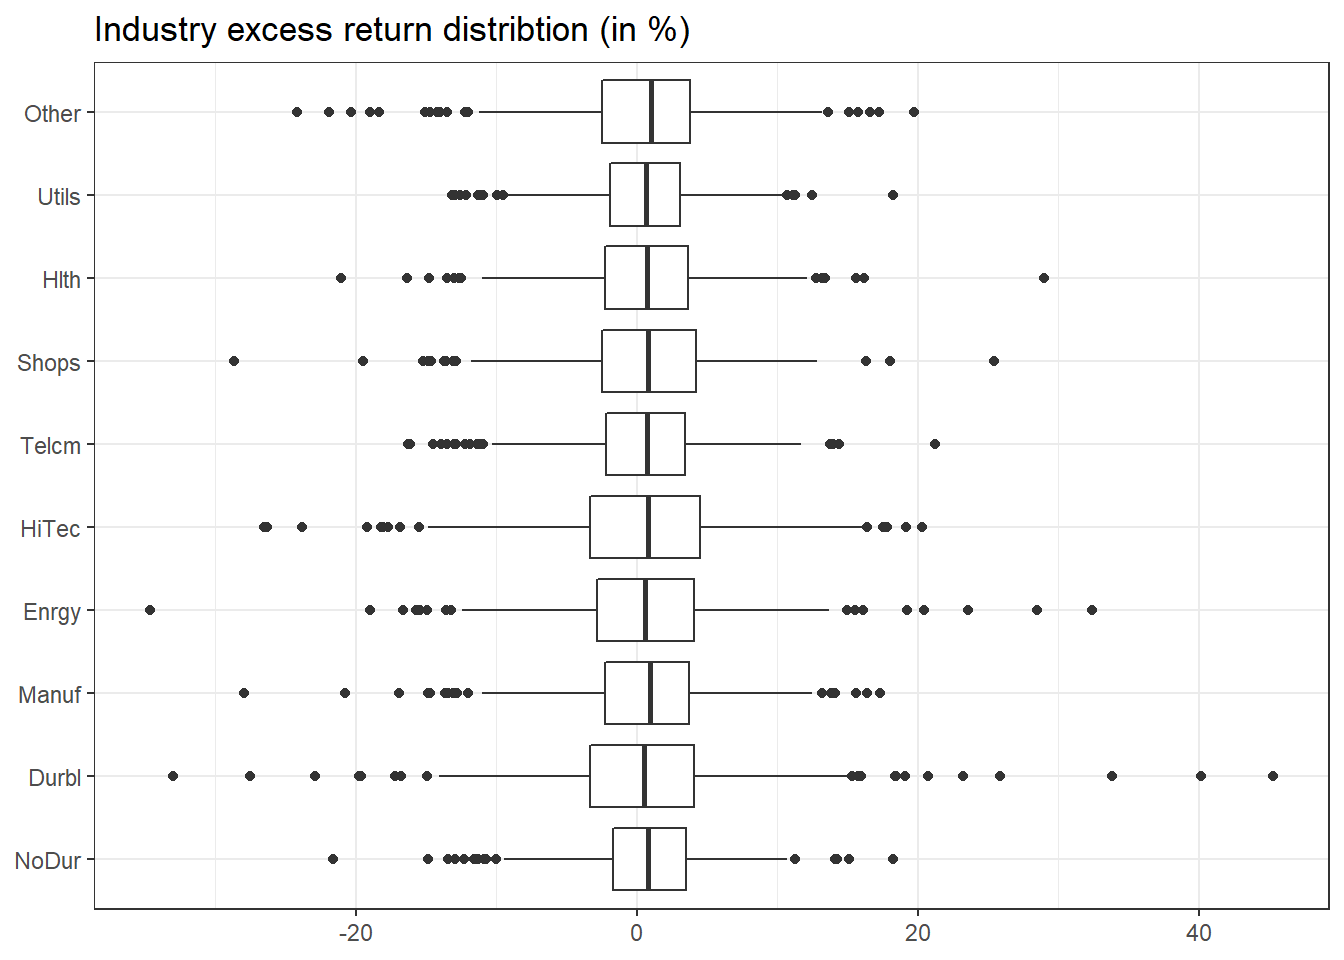
\includegraphics{40_factor_selection_with_machine_learning_files/figure-latex/industryreturns-1} \end{center}

\hypertarget{the-tidymodels-workflow}{%
\section{The tidymodels workflow}\label{the-tidymodels-workflow}}

To illustrate penalized linear regressions, we employ the \texttt{tidymodels} collection of packages for modeling and ML using \texttt{tidyverse} principles. You can simply use \texttt{install.packages("tidymodels")} to get access to all the related packages. We recommend checking out the work of Max Kuhn and Julia Silge: They continuously write on the great book `\href{https://www.tmwr.org/}{Tidy Modeling with R}' using tidy principles.

The \texttt{tidymodels} workflow encompasses the main stages of the modeling process: pre-processing of data, model fitting, and post-processing of results. As we demonstrate below, \texttt{tidymodels} provides efficient workflows that you can update with low effort.

Using the ideas of Ridge and Lasso regressions, the following example guides you through (i) pre-processing the data (data split and variable mutation), (ii) building models, (iii) fitting models, and (iv) tuning models to create the ``best'' possible predictions.

To start, we restrict our analysis to just one industry: Manufacturing. We first split the sample into a \emph{training} and a \emph{test} set.
For that purpose, \texttt{tidymodels} provides the function \texttt{initial\_time\_split} from the \texttt{rsample} package.
The split takes the last 20\% of the data as a test set, which is not used for any model tuning.
We use this test set to evaluate the predictive accuracy in an out-of-sample scenario.

\begin{Shaded}
\begin{Highlighting}[]
\NormalTok{split }\OtherTok{\textless{}{-}} \FunctionTok{initial\_time\_split}\NormalTok{(}
\NormalTok{  data }\SpecialCharTok{|}\ErrorTok{\textgreater{}}
    \FunctionTok{filter}\NormalTok{(industry }\SpecialCharTok{==} \StringTok{"Manuf"}\NormalTok{) }\SpecialCharTok{|}\ErrorTok{\textgreater{}}
    \FunctionTok{select}\NormalTok{(}\SpecialCharTok{{-}}\NormalTok{industry),}
  \AttributeTok{prop =} \DecValTok{4} \SpecialCharTok{/} \DecValTok{5}
\NormalTok{)}
\NormalTok{split}
\end{Highlighting}
\end{Shaded}

\begin{verbatim}
## <Training/Testing/Total>
## <517/130/647>
\end{verbatim}

The object \texttt{split} simply keeps track of the observations of the training and the test set.
We can call the training set with \texttt{training(split)}, while we can extract the test set with \texttt{testing(split)}.

\hypertarget{pre-process-data}{%
\subsection{Pre-process data}\label{pre-process-data}}

Recipes help you pre-process your data before training your model. Recipes are a series of pre-processing steps such as variable selection, transformation, or conversion of qualitative predictors to indicator variables. Each recipe starts with a \texttt{formula} that defines the general structure of the dataset and the role of each variable (regressor or dependent variable). For our dataset, our recipe contains the following steps before we fit any model:

\begin{itemize}
\tightlist
\item
  Our formula defines that we want to explain excess returns with all available predictors.
\item
  We exclude the column \emph{month} from the analysis.
\item
  We include all interaction terms between factors and macroeconomic predictors.
\item
  We demean and scale each regressor such that the standard deviation is one.
\end{itemize}

\begin{Shaded}
\begin{Highlighting}[]
\NormalTok{rec }\OtherTok{\textless{}{-}} \FunctionTok{recipe}\NormalTok{(ret }\SpecialCharTok{\textasciitilde{}}\NormalTok{ ., }\AttributeTok{data =} \FunctionTok{training}\NormalTok{(split)) }\SpecialCharTok{|}\ErrorTok{\textgreater{}}
  \FunctionTok{step\_rm}\NormalTok{(month) }\SpecialCharTok{|}\ErrorTok{\textgreater{}}
  \FunctionTok{step\_interact}\NormalTok{(}\AttributeTok{terms =} \SpecialCharTok{\textasciitilde{}} \FunctionTok{contains}\NormalTok{(}\StringTok{"factor"}\NormalTok{)}\SpecialCharTok{:}\FunctionTok{contains}\NormalTok{(}\StringTok{"macro"}\NormalTok{)) }\SpecialCharTok{|}\ErrorTok{\textgreater{}}
  \FunctionTok{step\_normalize}\NormalTok{(}\FunctionTok{all\_predictors}\NormalTok{()) }\SpecialCharTok{|}\ErrorTok{\textgreater{}}
  \FunctionTok{step\_center}\NormalTok{(ret, }\AttributeTok{skip =} \ConstantTok{TRUE}\NormalTok{)}
\end{Highlighting}
\end{Shaded}

A table of all available recipe steps can be found \href{https://www.tidymodels.org/find/recipes/}{here}. As of 2022, more than 150 different processing steps are available! One important point: The definition of a recipe does not trigger any calculations yet but rather provides a \emph{description} of the tasks to be applied. As a result, it is very easy to \emph{reuse} recipes for different models and thus make sure that the outcomes are comparable as they are based on the same input.
In the example above, it does not make a difference whether you use the input \texttt{data\ =\ training(split)} or \texttt{data\ =\ testing(split)}.
All that matters at this early stage are the column names and types.

We can apply the recipe to any data with a suitable structure. The code below combines two different functions: \texttt{prep} estimates the required parameters from a training set that can be applied to other data sets later. \texttt{bake} applies the processed computations to new data.

\begin{Shaded}
\begin{Highlighting}[]
\NormalTok{tmp\_data }\OtherTok{\textless{}{-}} \FunctionTok{bake}\NormalTok{(}\FunctionTok{prep}\NormalTok{(rec, }\FunctionTok{training}\NormalTok{(split)), }\AttributeTok{new\_data =} \FunctionTok{testing}\NormalTok{(split))}
\NormalTok{tmp\_data}
\end{Highlighting}
\end{Shaded}

\begin{verbatim}
## # A tibble: 130 x 126
##   factor_ff_rf factor_ff_mkt_excess factor_ff_smb
##          <dbl>                <dbl>         <dbl>
## 1        -1.92                0.644        0.298 
## 2        -1.88                1.27         0.387 
## 3        -1.88                0.341        1.43  
## 4        -1.88               -1.80        -0.0411
## 5        -1.88               -1.29        -0.627 
## # ... with 125 more rows, and 123 more variables:
## #   factor_ff_hml <dbl>, factor_q_me <dbl>,
## #   factor_q_ia <dbl>, factor_q_roe <dbl>,
## #   factor_q_eg <dbl>, macro_dp <dbl>, macro_dy <dbl>,
## #   macro_ep <dbl>, macro_de <dbl>, macro_svar <dbl>,
## #   macro_bm <dbl>, macro_ntis <dbl>, macro_tbl <dbl>,
## #   macro_lty <dbl>, macro_ltr <dbl>, ...
\end{verbatim}

Note that the resulting data contains the 130 observations from the test set and 126 columns. Why so many? Recall that the recipe states to compute every possible interaction term between the factors and predictors, which increases the dimension of the data matrix substantially.

You may ask at this stage: Why should I use a recipe instead of simply using the data wrangling commands such as \texttt{mutate} or \texttt{select}? \texttt{tidymodels} beauty is that a lot is happening under the hood. Recall, that for the simple scaling step, you actually have to compute the standard deviation of each column, then \emph{store} this value, and apply the identical transformation to a different dataset, e.g., \texttt{testing(split)}. A prepped \texttt{recipe} stores these values and hands them on once you \texttt{bake} a novel dataset. Easy as pie with \texttt{tidymodels}, isn't it?

\hypertarget{build-a-model}{%
\subsection{Build a model}\label{build-a-model}}

Next, we can build an actual model based on our pre-processed data. In line with the definition above, we estimate regression coefficients of a Lasso regression such that we get
\[\begin{aligned}\hat\beta_\lambda^\text{Lasso} = \arg\min_\beta \left(Y - X\beta\right)'\left(Y - X\beta\right) + \lambda\sum\limits_{k=1}^K|\beta_k|.\end{aligned}\] We want to emphasize that the \texttt{tidymodels} workflow for \emph{any} model is very similar, irrespective of the specific model. As you will see further below, it is straightforward to fit Ridge regression coefficients and - later - Neural networks or Random forests with basically the same code. The structure is always as follows: create a so-called \texttt{workflow} and use the \texttt{fit} function. A table with all available model APIs is available \href{https://www.tidymodels.org/find/parsnip/}{here}.
For now, we start with the linear regression model with a given value for the penalty factor \(\lambda\). In the setup below, \texttt{mixture} denotes the value of \(\rho\), hence setting \texttt{mixture\ =\ 1} implies the Lasso.

\begin{Shaded}
\begin{Highlighting}[]
\NormalTok{lm\_model }\OtherTok{\textless{}{-}} \FunctionTok{linear\_reg}\NormalTok{(}
  \AttributeTok{penalty =} \FloatTok{0.0001}\NormalTok{,}
  \AttributeTok{mixture =} \DecValTok{1}
\NormalTok{) }\SpecialCharTok{|}\ErrorTok{\textgreater{}}
  \FunctionTok{set\_engine}\NormalTok{(}\StringTok{"glmnet"}\NormalTok{, }\AttributeTok{intercept =} \ConstantTok{FALSE}\NormalTok{)}
\end{Highlighting}
\end{Shaded}

That's it - we are done! The object \texttt{lm\_model} contains the definition of our model with all required information. Note that \texttt{set\_engine("glmnet")} indicates the API character of the \texttt{tidymodels} workflow: Under the hood, the package \texttt{glmnet} is doing the heavy lifting, while \texttt{linear\_reg} provides a unified framework to collect the inputs. The \texttt{workflow} ends with combining everything necessary for the (serious) data science workflow, namely, a recipe and a model.

\begin{Shaded}
\begin{Highlighting}[]
\NormalTok{lm\_fit }\OtherTok{\textless{}{-}} \FunctionTok{workflow}\NormalTok{() }\SpecialCharTok{|}\ErrorTok{\textgreater{}}
  \FunctionTok{add\_recipe}\NormalTok{(rec) }\SpecialCharTok{|}\ErrorTok{\textgreater{}}
  \FunctionTok{add\_model}\NormalTok{(lm\_model)}
\NormalTok{lm\_fit}
\end{Highlighting}
\end{Shaded}

\begin{verbatim}
## == Workflow ===========================================
## Preprocessor: Recipe
## Model: linear_reg()
## 
## -- Preprocessor ---------------------------------------
## 4 Recipe Steps
## 
## * step_rm()
## * step_interact()
## * step_normalize()
## * step_center()
## 
## -- Model ----------------------------------------------
## Linear Regression Model Specification (regression)
## 
## Main Arguments:
##   penalty = 1e-04
##   mixture = 1
## 
## Engine-Specific Arguments:
##   intercept = FALSE
## 
## Computational engine: glmnet
\end{verbatim}

\hypertarget{fit-a-model}{%
\subsection{Fit a model}\label{fit-a-model}}

With the \texttt{workflow} from above, we are ready to use \texttt{fit}. Typically, we use training data to fit the model.
The training data is pre-processed according to our recipe steps, and the Lasso regression coefficients are computed.
First, we focus on the predicted values \(\hat{y}_t = x_t\hat\beta^\text{Lasso}.\) The figure below illustrates the projections for the \emph{entire} time series of the Manufacturing industry portfolio returns. The grey area indicates the out-of-sample period, which we did not use to fit the model.

\begin{Shaded}
\begin{Highlighting}[]
\NormalTok{predicted\_values }\OtherTok{\textless{}{-}}\NormalTok{ lm\_fit }\SpecialCharTok{|}\ErrorTok{\textgreater{}}
  \FunctionTok{fit}\NormalTok{(}\AttributeTok{data =} \FunctionTok{training}\NormalTok{(split)) }\SpecialCharTok{|}\ErrorTok{\textgreater{}}
  \FunctionTok{predict}\NormalTok{(data }\SpecialCharTok{|}\ErrorTok{\textgreater{}} \FunctionTok{filter}\NormalTok{(industry }\SpecialCharTok{==} \StringTok{"Manuf"}\NormalTok{)) }\SpecialCharTok{|}\ErrorTok{\textgreater{}}
  \FunctionTok{bind\_cols}\NormalTok{(data }\SpecialCharTok{|}\ErrorTok{\textgreater{}} \FunctionTok{filter}\NormalTok{(industry }\SpecialCharTok{==} \StringTok{"Manuf"}\NormalTok{)) }\SpecialCharTok{|}\ErrorTok{\textgreater{}}
  \FunctionTok{select}\NormalTok{(month,}
    \StringTok{"Fitted value"} \OtherTok{=}\NormalTok{ .pred,}
    \StringTok{"Realization"} \OtherTok{=}\NormalTok{ ret}
\NormalTok{  ) }\SpecialCharTok{|}\ErrorTok{\textgreater{}}
  \FunctionTok{pivot\_longer}\NormalTok{(}\SpecialCharTok{{-}}\NormalTok{month, }\AttributeTok{names\_to =} \StringTok{"Variable"}\NormalTok{)}

\NormalTok{predicted\_values }\SpecialCharTok{|}\ErrorTok{\textgreater{}}
  \FunctionTok{ggplot}\NormalTok{(}\FunctionTok{aes}\NormalTok{(}\AttributeTok{x =}\NormalTok{ month, }\AttributeTok{y =}\NormalTok{ value, }\AttributeTok{color =}\NormalTok{ Variable)) }\SpecialCharTok{+}
  \FunctionTok{geom\_line}\NormalTok{() }\SpecialCharTok{+}
  \FunctionTok{labs}\NormalTok{(}
    \AttributeTok{x =} \ConstantTok{NULL}\NormalTok{,}
    \AttributeTok{y =} \ConstantTok{NULL}\NormalTok{,}
    \AttributeTok{color =} \ConstantTok{NULL}\NormalTok{,}
    \AttributeTok{title =} \StringTok{"Monthly realized and fitted manufacturing industry risk premia"}
\NormalTok{  ) }\SpecialCharTok{+}
  \FunctionTok{scale\_x\_date}\NormalTok{(}
    \AttributeTok{breaks =} \ControlFlowTok{function}\NormalTok{(x) }\FunctionTok{seq.Date}\NormalTok{(}\AttributeTok{from =} \FunctionTok{min}\NormalTok{(x), }\AttributeTok{to =} \FunctionTok{max}\NormalTok{(x), }\AttributeTok{by =} \StringTok{"5 years"}\NormalTok{),}
    \AttributeTok{minor\_breaks =} \ControlFlowTok{function}\NormalTok{(x) }\FunctionTok{seq.Date}\NormalTok{(}\AttributeTok{from =} \FunctionTok{min}\NormalTok{(x), }\AttributeTok{to =} \FunctionTok{max}\NormalTok{(x), }\AttributeTok{by =} \StringTok{"1 years"}\NormalTok{),}
    \AttributeTok{expand =} \FunctionTok{c}\NormalTok{(}\DecValTok{0}\NormalTok{, }\DecValTok{0}\NormalTok{),}
    \AttributeTok{labels =} \FunctionTok{date\_format}\NormalTok{(}\StringTok{"\%Y"}\NormalTok{)}
\NormalTok{  ) }\SpecialCharTok{+}
  \FunctionTok{scale\_y\_continuous}\NormalTok{(}
    \AttributeTok{labels =}\NormalTok{ percent}
\NormalTok{  ) }\SpecialCharTok{+}
  \FunctionTok{annotate}\NormalTok{(}\StringTok{"rect"}\NormalTok{,}
    \AttributeTok{xmin =} \FunctionTok{testing}\NormalTok{(split) }\SpecialCharTok{|}\ErrorTok{\textgreater{}} \FunctionTok{pull}\NormalTok{(month) }\SpecialCharTok{|}\ErrorTok{\textgreater{}} \FunctionTok{min}\NormalTok{(),}
    \AttributeTok{xmax =} \FunctionTok{testing}\NormalTok{(split) }\SpecialCharTok{|}\ErrorTok{\textgreater{}} \FunctionTok{pull}\NormalTok{(month) }\SpecialCharTok{|}\ErrorTok{\textgreater{}} \FunctionTok{max}\NormalTok{(),}
    \AttributeTok{ymin =} \SpecialCharTok{{-}}\ConstantTok{Inf}\NormalTok{, }\AttributeTok{ymax =} \ConstantTok{Inf}\NormalTok{,}
    \AttributeTok{alpha =} \FloatTok{0.5}\NormalTok{, }\AttributeTok{fill =} \StringTok{"grey70"}
\NormalTok{  )}
\end{Highlighting}
\end{Shaded}

\begin{center}\includegraphics{40_factor_selection_with_machine_learning_files/figure-latex/unnamed-chunk-9-1} \end{center}

What do the estimated coefficients look like? To analyze these values and to illustrate the difference between the \texttt{tidymodels} workflow and the underlying \texttt{glmnet} package, it is worth computing the coefficients \(\hat\beta^\text{Lasso}\) directly. The code below estimates the coefficients for the Lasso and Ridge regression for the processed training data sample. Note that \texttt{glmnet} actually takes a vector \texttt{y} and the matrix of regressors \(X\) as input. Moreover, \texttt{glmnet} requires choosing the penalty parameter \(\alpha\), which corresponds to \(\rho\) in the notation above. When using the \texttt{tidymodels} model API, such details do not need consideration.

\begin{Shaded}
\begin{Highlighting}[]
\NormalTok{x }\OtherTok{\textless{}{-}}\NormalTok{ tmp\_data }\SpecialCharTok{|}\ErrorTok{\textgreater{}}
  \FunctionTok{select}\NormalTok{(}\SpecialCharTok{{-}}\NormalTok{ret) }\SpecialCharTok{|}\ErrorTok{\textgreater{}}
  \FunctionTok{as.matrix}\NormalTok{()}
\NormalTok{y }\OtherTok{\textless{}{-}}\NormalTok{ tmp\_data }\SpecialCharTok{|}\ErrorTok{\textgreater{}} \FunctionTok{pull}\NormalTok{(ret)}

\NormalTok{fit\_lasso }\OtherTok{\textless{}{-}} \FunctionTok{glmnet}\NormalTok{(}
  \AttributeTok{x =}\NormalTok{ x,}
  \AttributeTok{y =}\NormalTok{ y,}
  \AttributeTok{alpha =} \DecValTok{1}\NormalTok{,}
  \AttributeTok{intercept =} \ConstantTok{FALSE}\NormalTok{,}
  \AttributeTok{standardize =} \ConstantTok{FALSE}\NormalTok{,}
  \AttributeTok{lambda.min.ratio =} \DecValTok{0}
\NormalTok{)}

\NormalTok{fit\_ridge }\OtherTok{\textless{}{-}} \FunctionTok{glmnet}\NormalTok{(}
  \AttributeTok{x =}\NormalTok{ x,}
  \AttributeTok{y =}\NormalTok{ y,}
  \AttributeTok{alpha =} \DecValTok{0}\NormalTok{,}
  \AttributeTok{intercept =} \ConstantTok{FALSE}\NormalTok{,}
  \AttributeTok{standardize =} \ConstantTok{FALSE}\NormalTok{,}
  \AttributeTok{lambda.min.ratio =} \DecValTok{0}
\NormalTok{)}
\end{Highlighting}
\end{Shaded}

The objects \texttt{fit\_lasso} and \texttt{fit\_ridge} contain an entire sequence of estimated coefficients for multiple values of the penalty factor \(\lambda\). The figure below illustrates the trajectories of the regression coefficients as a function of the penalty factor. Both Lasso and Ridge coefficients converge to zero as the penalty factor increases.

\begin{Shaded}
\begin{Highlighting}[]
\FunctionTok{bind\_rows}\NormalTok{(}
  \FunctionTok{tidy}\NormalTok{(fit\_lasso) }\SpecialCharTok{|}\ErrorTok{\textgreater{}} \FunctionTok{mutate}\NormalTok{(}\AttributeTok{Model =} \StringTok{"Lasso"}\NormalTok{),}
  \FunctionTok{tidy}\NormalTok{(fit\_ridge) }\SpecialCharTok{|}\ErrorTok{\textgreater{}} \FunctionTok{mutate}\NormalTok{(}\AttributeTok{Model =} \StringTok{"Ridge"}\NormalTok{)}
\NormalTok{) }\SpecialCharTok{|}\ErrorTok{\textgreater{}}
  \FunctionTok{rename}\NormalTok{(}\StringTok{"Variable"} \OtherTok{=}\NormalTok{ term) }\SpecialCharTok{|}\ErrorTok{\textgreater{}}
  \FunctionTok{ggplot}\NormalTok{(}\FunctionTok{aes}\NormalTok{(}\AttributeTok{x =}\NormalTok{ lambda, }\AttributeTok{y =}\NormalTok{ estimate, }\AttributeTok{color =}\NormalTok{ Variable)) }\SpecialCharTok{+}
  \FunctionTok{geom\_line}\NormalTok{() }\SpecialCharTok{+}
  \FunctionTok{scale\_x\_log10}\NormalTok{() }\SpecialCharTok{+}
  \FunctionTok{facet\_wrap}\NormalTok{(}\SpecialCharTok{\textasciitilde{}}\NormalTok{Model, }\AttributeTok{scales =} \StringTok{"free\_x"}\NormalTok{) }\SpecialCharTok{+}
  \FunctionTok{labs}\NormalTok{(}
    \AttributeTok{x =} \StringTok{"Lambda"}\NormalTok{, }\AttributeTok{y =} \ConstantTok{NULL}\NormalTok{,}
    \AttributeTok{title =} \StringTok{"Estimated Coefficients paths as a}
\StringTok{    function of the penalty factor"}
\NormalTok{  ) }\SpecialCharTok{+}
  \FunctionTok{theme}\NormalTok{(}\AttributeTok{legend.position =} \StringTok{"none"}\NormalTok{)}
\end{Highlighting}
\end{Shaded}

\begin{center}\includegraphics{40_factor_selection_with_machine_learning_files/figure-latex/unnamed-chunk-11-1} \end{center}

One word of caution: The package \texttt{glmnet} computes estimates of the coefficients \(\hat\beta\) based on numerical optimization procedures.
As a result, the estimated coefficients for the \href{https://parsnip.tidymodels.org/reference/glmnet-details.html}{special case} with no regularization (\(\lambda = 0\)) can deviate from the standard OLS estimates.

\hypertarget{tune-a-model}{%
\subsection{Tune a model}\label{tune-a-model}}

To compute \(\hat\beta_\lambda^\text{Lasso}\) , we simply imposed a value for the penalty hyperparameter \(\lambda\). Model tuning is the process of optimally selecting such hyperparameters. \texttt{tidymodels} provides extensive tuning options based on so-called \emph{cross-validation}. Again, we refer to any treatment of cross-validation to get a more detailed discussion of the statistical underpinnings. Here we focus on the general idea and the implementation with \texttt{tidymodels}.

The goal for choosing \(\lambda\) (or any other hyperparameter, e.g., \(\rho\)) is to find a way to produce predictors \(\hat{Y}\) for an outcome \(Y\) that minimizes the mean squared prediction error \(\text{MSPE} = E\left( \frac{1}{T}\sum_{t=1}^T (\hat{y}_t - y_t)^2 \right)\). Unfortunately, the MSPE is not directly observable. We can only compute an estimate because our data is random and because we do not observe the entire population.

Obviously, if we train an algorithm on the same data that we use to compute the error, our estimate \(\hat{\text{MSPE}}\) would indicate way better predictive accuracy than what we can expect in real out-of-sample data. The result is called overfitting.

Cross-validation is a technique that allows us to alleviate this problem. We approximate the true MSPE as the average of many mean squared prediction errors obtained by creating predictions for \(K\) new random samples of the data, none of them used to train the algorithm \(\frac{1}{K} \sum_{k=1}^K \frac{1}{T}\sum_{t=1}^T \left(\hat{y}_t^k - y_t^k\right)^2\). In practice, this is done by carving out a piece of our data and pretending it is an independent sample. We again divide the data into a training set and a test set. The MSPE on the test set is our measure for actual predictive ability, while we use the training set to fit models with the aim to find the \emph{optimal} hyperparameter values. To do so, we further divide our training sample into (several) subsets, fit our model for a grid of potential hyperparameter values (e.g., \(\lambda\)), and evaluate the predictive accuracy on an \emph{independent} sample. This works as follows:

\begin{enumerate}
\def\labelenumi{\arabic{enumi}.}
\tightlist
\item
  Specify a grid of hyperparameters.
\item
  Obtain predictors \(\hat{y}_i(\lambda)\) to denote the predictors for the used parameters \(\lambda\).
\item
  Compute \[
  \text{MSPE}(\lambda) = \frac{1}{K} \sum_{k=1}^K \frac{1}{T}\sum_{t=1}^T \left(\hat{y}_t^k(\lambda) - y_t^k\right)^2 
  \] With K-fold cross-validation, we do this computation \(K\) times. Simply pick a validation set with \(M=T/K\) observations at random and think of these as random samples \(y_1^k, \dots, y_{\tilde{T}}^k\), with \(k=1\).
\end{enumerate}

How should you pick \(K\)? Large values of \(K\) are preferable because the training data better imitates the original data. However, larger values of \(K\) will have much higher computation time.
\texttt{tidymodels} provides all required tools to conduct \(K\)-fold cross-validation. We just have to update our model specification and let \texttt{tidymodels} know which parameters to tune. In our case, we specify the penalty factor \(\lambda\) as well as the mixing factor \(\rho\) as \emph{free} parameters. Note that it is simple to change an existing \texttt{workflow} with \texttt{update\_model}.

\begin{Shaded}
\begin{Highlighting}[]
\NormalTok{lm\_model }\OtherTok{\textless{}{-}} \FunctionTok{linear\_reg}\NormalTok{(}
  \AttributeTok{penalty =} \FunctionTok{tune}\NormalTok{(),}
  \AttributeTok{mixture =} \FunctionTok{tune}\NormalTok{()}
\NormalTok{) }\SpecialCharTok{|}\ErrorTok{\textgreater{}}
  \FunctionTok{set\_engine}\NormalTok{(}\StringTok{"glmnet"}\NormalTok{)}

\NormalTok{lm\_fit }\OtherTok{\textless{}{-}}\NormalTok{ lm\_fit }\SpecialCharTok{|}\ErrorTok{\textgreater{}}
  \FunctionTok{update\_model}\NormalTok{(lm\_model)}
\end{Highlighting}
\end{Shaded}

For our sample, we consider a time-series cross-validation sample. This means that we tune our models with 20 random samples of length five years with a validation period of four years. For a grid of possible hyperparameters, we then fit the model for each fold and evaluate \(\hat{\text{MSPE}}\) in the corresponding validation set. Finally, we select the model specification with the lowest MSPE in the validation set. First, we define the cross-validation folds based on our training data only.

\begin{Shaded}
\begin{Highlighting}[]
\NormalTok{data\_folds }\OtherTok{\textless{}{-}} \FunctionTok{time\_series\_cv}\NormalTok{(}
  \AttributeTok{data        =} \FunctionTok{training}\NormalTok{(split),}
  \AttributeTok{date\_var    =}\NormalTok{ month,}
  \AttributeTok{initial     =} \StringTok{"5 years"}\NormalTok{,}
  \AttributeTok{assess      =} \StringTok{"48 months"}\NormalTok{,}
  \AttributeTok{cumulative  =} \ConstantTok{FALSE}\NormalTok{,}
  \AttributeTok{slice\_limit =} \DecValTok{20}
\NormalTok{)}
\end{Highlighting}
\end{Shaded}

Then, we evaluate the performance for a grid of different penalty values. \texttt{tidymodels} provides functionalities to construct a suitable grid of hyperparameters with \texttt{grid\_regular}. The code chunk below creates a \(10 \times 3\) hyperparameters grid. Then, the function \texttt{tune\_grid} evaluates all the models for each fold.

\begin{Shaded}
\begin{Highlighting}[]
\NormalTok{lm\_tune }\OtherTok{\textless{}{-}}\NormalTok{ lm\_fit }\SpecialCharTok{|}\ErrorTok{\textgreater{}}
  \FunctionTok{tune\_grid}\NormalTok{(}
    \AttributeTok{resample =}\NormalTok{ data\_folds,}
    \AttributeTok{grid =} \FunctionTok{grid\_regular}\NormalTok{(}\FunctionTok{penalty}\NormalTok{(), }\FunctionTok{mixture}\NormalTok{(), }\AttributeTok{levels =} \FunctionTok{c}\NormalTok{(}\DecValTok{10}\NormalTok{, }\DecValTok{3}\NormalTok{)),}
    \AttributeTok{metrics =} \FunctionTok{metric\_set}\NormalTok{(rmse)}
\NormalTok{  )}
\end{Highlighting}
\end{Shaded}

After the tuning process, we collect the evaluation metrics (the root mean-squared error in our example) to identify the \emph{optimal} model. The figure illustrates the average validation set's root mean-squared error for each value of \(\lambda\) and \(\rho\).

\begin{Shaded}
\begin{Highlighting}[]
\FunctionTok{autoplot}\NormalTok{(lm\_tune) }\SpecialCharTok{+}
  \FunctionTok{labs}\NormalTok{(}
    \AttributeTok{y =} \StringTok{"Root mean{-}squared prediction error"}\NormalTok{,}
    \AttributeTok{title =} \StringTok{"MSPE for Manufacturing excess returns"}\NormalTok{,}
    \AttributeTok{subtitle =} \StringTok{"Lasso (1.0), Ridge (0.0), and Elastic Net (0.5) with different levels of regularization."}
\NormalTok{  )}
\end{Highlighting}
\end{Shaded}

\begin{center}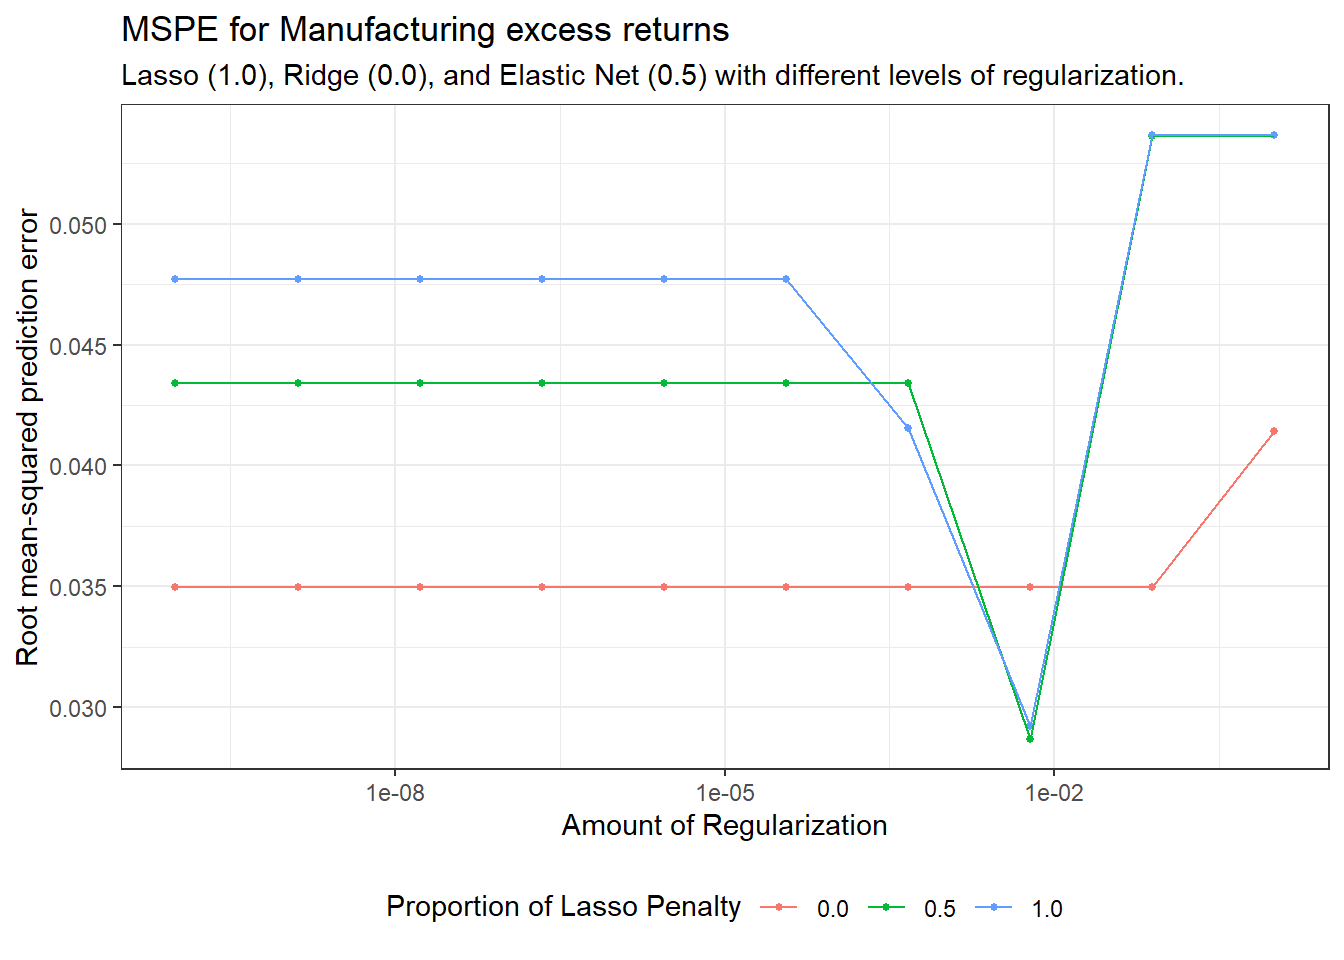
\includegraphics{40_factor_selection_with_machine_learning_files/figure-latex/unnamed-chunk-15-1} \end{center}

The figure shows that the cross-validated mean squared prediction error drops for Lasso and Elastic Net and spikes afterward. For Ridge regression, the MSPE increases above a certain threshold. Recall that the larger the regularization, the more restricted the model becomes. Thus, we would choose the model with the lowest MSPE, which exhibits some intermediate level of regularization.

\hypertarget{parallelized-workflow}{%
\subsection{Parallelized workflow}\label{parallelized-workflow}}

Our starting point was the question: Which factors determine industry returns? To illustrate the entire workflow, we now run the penalized regressions for all ten industries. We want to identify relevant variables by fitting Lasso models for each industry returns time series. More specifically, we perform cross-validation for each industry to identify the optimal penalty factor \(\lambda\). Then, we use the set of \texttt{finalize\_*}-functions that take a list or tibble of tuning parameter values and update objects with those values. After determining the best model, we compute the final fit on the entire training set and analyze the estimated coefficients.

First, we define the Lasso model with one tuning parameter.

\begin{Shaded}
\begin{Highlighting}[]
\NormalTok{lasso\_model }\OtherTok{\textless{}{-}} \FunctionTok{linear\_reg}\NormalTok{(}
  \AttributeTok{penalty =} \FunctionTok{tune}\NormalTok{(),}
  \AttributeTok{mixture =} \DecValTok{1}
\NormalTok{) }\SpecialCharTok{|}\ErrorTok{\textgreater{}}
  \FunctionTok{set\_engine}\NormalTok{(}\StringTok{"glmnet"}\NormalTok{)}

\NormalTok{lm\_fit }\OtherTok{\textless{}{-}}\NormalTok{ lm\_fit }\SpecialCharTok{|}\ErrorTok{\textgreater{}}
  \FunctionTok{update\_model}\NormalTok{(lasso\_model)}
\end{Highlighting}
\end{Shaded}

The following task can be easily parallelized to reduce computing time substantially. We use the parallelization capabilities of \texttt{furrr}. Note that we can also just recycle all the steps from above and collect them in a function.

\begin{Shaded}
\begin{Highlighting}[]
\NormalTok{select\_variables }\OtherTok{\textless{}{-}} \ControlFlowTok{function}\NormalTok{(input) \{}
  \CommentTok{\# Split into training and testing data}
\NormalTok{  split }\OtherTok{\textless{}{-}} \FunctionTok{initial\_time\_split}\NormalTok{(input, }\AttributeTok{prop =} \DecValTok{4} \SpecialCharTok{/} \DecValTok{5}\NormalTok{)}

  \CommentTok{\# Data folds for cross{-}validation}
\NormalTok{  data\_folds }\OtherTok{\textless{}{-}} \FunctionTok{time\_series\_cv}\NormalTok{(}
    \AttributeTok{data =} \FunctionTok{training}\NormalTok{(split),}
    \AttributeTok{date\_var =}\NormalTok{ month,}
    \AttributeTok{initial =} \StringTok{"5 years"}\NormalTok{,}
    \AttributeTok{assess =} \StringTok{"48 months"}\NormalTok{,}
    \AttributeTok{cumulative =} \ConstantTok{FALSE}\NormalTok{,}
    \AttributeTok{slice\_limit =} \DecValTok{20}
\NormalTok{  )}

  \CommentTok{\# Model tuning with the Lasso model}
\NormalTok{  lm\_tune }\OtherTok{\textless{}{-}}\NormalTok{ lm\_fit }\SpecialCharTok{|}\ErrorTok{\textgreater{}}
    \FunctionTok{tune\_grid}\NormalTok{(}
      \AttributeTok{resample =}\NormalTok{ data\_folds,}
      \AttributeTok{grid =} \FunctionTok{grid\_regular}\NormalTok{(}\FunctionTok{penalty}\NormalTok{(), }\AttributeTok{levels =} \FunctionTok{c}\NormalTok{(}\DecValTok{10}\NormalTok{)),}
      \AttributeTok{metrics =} \FunctionTok{metric\_set}\NormalTok{(rmse)}
\NormalTok{    )}

  \CommentTok{\# Finalizing: Identify the best model and fit with the training data}
\NormalTok{  lasso\_lowest\_rmse }\OtherTok{\textless{}{-}}\NormalTok{ lm\_tune }\SpecialCharTok{|}\ErrorTok{\textgreater{}} \FunctionTok{select\_by\_one\_std\_err}\NormalTok{(}\StringTok{"rmse"}\NormalTok{)}
\NormalTok{  lasso\_final }\OtherTok{\textless{}{-}} \FunctionTok{finalize\_workflow}\NormalTok{(lm\_fit, lasso\_lowest\_rmse)}
\NormalTok{  lasso\_final\_fit }\OtherTok{\textless{}{-}} \FunctionTok{last\_fit}\NormalTok{(lasso\_final, split, }\AttributeTok{metrics =} \FunctionTok{metric\_set}\NormalTok{(rmse))}

  \CommentTok{\# Extract the estimated coefficients}
\NormalTok{  lasso\_final\_fit }\SpecialCharTok{|}\ErrorTok{\textgreater{}}
    \FunctionTok{extract\_fit\_parsnip}\NormalTok{() }\SpecialCharTok{|}\ErrorTok{\textgreater{}}
    \FunctionTok{tidy}\NormalTok{() }\SpecialCharTok{|}\ErrorTok{\textgreater{}}
    \FunctionTok{mutate}\NormalTok{(}
      \AttributeTok{term =} \FunctionTok{str\_remove\_all}\NormalTok{(term, }\StringTok{"factor\_|macro\_|industry\_"}\NormalTok{)}
\NormalTok{    )}
\NormalTok{\}}

\CommentTok{\# Parallelization}
\FunctionTok{plan}\NormalTok{(multisession, }\AttributeTok{workers =} \FunctionTok{availableCores}\NormalTok{())}

\CommentTok{\# Computation by industry}
\NormalTok{selected\_factors }\OtherTok{\textless{}{-}}\NormalTok{ data }\SpecialCharTok{|}\ErrorTok{\textgreater{}}
  \FunctionTok{nest}\NormalTok{(}\AttributeTok{data =} \SpecialCharTok{{-}}\NormalTok{industry) }\SpecialCharTok{|}\ErrorTok{\textgreater{}}
  \FunctionTok{mutate}\NormalTok{(}\AttributeTok{selected\_variables =} \FunctionTok{future\_map}\NormalTok{(data, select\_variables,}
    \AttributeTok{.options =} \FunctionTok{furrr\_options}\NormalTok{(}\AttributeTok{seed =} \ConstantTok{TRUE}\NormalTok{)}
\NormalTok{  ))}
\end{Highlighting}
\end{Shaded}

What has just happened? In principle, exactly the same as before but instead of computing the Lasso coefficients for one industry, we did it for ten in parallel. The final option \texttt{seed\ =\ TRUE} is required to make the cross-validation process reproducible.
Now, we just have to do some housekeeping and keep only variables that Lasso does \emph{not} set to zero. We illustrate the results in a heat map.

\begin{Shaded}
\begin{Highlighting}[]
\NormalTok{selected\_factors }\SpecialCharTok{|}\ErrorTok{\textgreater{}}
  \FunctionTok{unnest}\NormalTok{(selected\_variables) }\SpecialCharTok{|}\ErrorTok{\textgreater{}}
  \FunctionTok{filter}\NormalTok{(}
\NormalTok{    term }\SpecialCharTok{!=} \StringTok{"(Intercept)"}\NormalTok{,}
\NormalTok{    estimate }\SpecialCharTok{!=} \DecValTok{0}
\NormalTok{  ) }\SpecialCharTok{|}\ErrorTok{\textgreater{}}
  \FunctionTok{add\_count}\NormalTok{(term) }\SpecialCharTok{|}\ErrorTok{\textgreater{}}
  \FunctionTok{mutate}\NormalTok{(}
    \AttributeTok{term =} \FunctionTok{str\_remove\_all}\NormalTok{(term, }\StringTok{"NA|ff\_|q\_"}\NormalTok{),}
    \AttributeTok{term =} \FunctionTok{str\_replace\_all}\NormalTok{(term, }\StringTok{"\_x\_"}\NormalTok{, }\StringTok{" "}\NormalTok{),}
    \AttributeTok{term =} \FunctionTok{fct\_reorder}\NormalTok{(}\FunctionTok{as\_factor}\NormalTok{(term), n),}
    \AttributeTok{term =} \FunctionTok{fct\_lump\_min}\NormalTok{(term, }\AttributeTok{min =} \DecValTok{2}\NormalTok{),}
    \AttributeTok{selected =} \DecValTok{1}
\NormalTok{  ) }\SpecialCharTok{|}\ErrorTok{\textgreater{}}
  \FunctionTok{filter}\NormalTok{(term }\SpecialCharTok{!=} \StringTok{"Other"}\NormalTok{) }\SpecialCharTok{|}\ErrorTok{\textgreater{}}
  \FunctionTok{mutate}\NormalTok{(}\AttributeTok{term =} \FunctionTok{fct\_drop}\NormalTok{(term)) }\SpecialCharTok{|}\ErrorTok{\textgreater{}}
  \FunctionTok{complete}\NormalTok{(industry, term, }\AttributeTok{fill =} \FunctionTok{list}\NormalTok{(}\AttributeTok{selected =} \DecValTok{0}\NormalTok{)) }\SpecialCharTok{|}\ErrorTok{\textgreater{}}
  \FunctionTok{ggplot}\NormalTok{(}\FunctionTok{aes}\NormalTok{(industry,}
\NormalTok{    term,}
    \AttributeTok{fill =} \FunctionTok{as\_factor}\NormalTok{(selected)}
\NormalTok{  )) }\SpecialCharTok{+}
  \FunctionTok{geom\_tile}\NormalTok{() }\SpecialCharTok{+}
  \FunctionTok{scale\_x\_discrete}\NormalTok{(}\AttributeTok{guide =} \FunctionTok{guide\_axis}\NormalTok{(}\AttributeTok{angle =} \DecValTok{70}\NormalTok{)) }\SpecialCharTok{+}
  \FunctionTok{scale\_fill\_manual}\NormalTok{(}\AttributeTok{values =} \FunctionTok{c}\NormalTok{(}\StringTok{"white"}\NormalTok{, }\StringTok{"cornflowerblue"}\NormalTok{)) }\SpecialCharTok{+}
  \FunctionTok{theme}\NormalTok{(}\AttributeTok{legend.position =} \StringTok{"None"}\NormalTok{) }\SpecialCharTok{+}
  \FunctionTok{labs}\NormalTok{(}
    \AttributeTok{x =} \ConstantTok{NULL}\NormalTok{, }\AttributeTok{y =} \ConstantTok{NULL}\NormalTok{,}
    \AttributeTok{title =} \StringTok{"Selected variables for different industries"}
\NormalTok{  )}
\end{Highlighting}
\end{Shaded}

\begin{center}\includegraphics{40_factor_selection_with_machine_learning_files/figure-latex/unnamed-chunk-18-1} \end{center}

The heat map conveys two main insights. First, we see a lot of white, which means that many factors, macroeconomic variables, and interaction terms are not relevant for explaining the cross-section of returns across the industry portfolios. In fact, only the market factor and the return-on-equity factor play a role for several industries. Second, there seems to be quite some heterogeneity across different industries. While not even the market factor is selected by Lasso for Utilities (which means the proposed model essentially just contains an intercept), many factors are selected for, e.g., High-Tech and Energy, but they do not coincide at all. In other words, there seems to be a clear picture that we do not need many factors, but Lasso does not provide conses across industries when it comes to pricing abilities.

\hypertarget{exercises-8}{%
\section{Exercises}\label{exercises-8}}

\begin{enumerate}
\def\labelenumi{\arabic{enumi}.}
\tightlist
\item
  Write a function that requires three inputs, namely, \texttt{y} (a \(T\) vector), \texttt{X} (a \((T \times K)\) matrix), and \texttt{lambda} and then returns the \textbf{Ridge} estimator (a \(K\) vector) for a given penalization parameter \(\lambda\). Recall that the intercept should not be penalized. Therefore, your function should indicate whether \(X\) contains a vector of ones as the first column, which should be exempt from the \(L_2\) penalty.
\item
  Compute the \(L_2\) norm (\(\beta'\beta\)) for the regression coefficients based on the predictive regression from the previous exercise for a range of \(\lambda\)'s and illustrate the effect of penalization in a suitable figure.
\item
  Now, write a function that requires three inputs, namely,\texttt{y} (a \(T\) vector), \texttt{X} (a \((T \times K)\) matrix), and 'lambda` and then returns the \textbf{Lasso} estimator (a \(K\) vector) for a given penalization parameter \(\lambda\). Recall that the intercept should not be penalized. Therefore, your function should indicate whether \(X\) contains a vector of ones as the first column, which should be exempt from the \(L_1\) penalty.
\item
  After you understand what Ridge and Lasso regressions are doing, familiarize yourself with the \texttt{glmnet()} package's documentation. It is a thoroughly tested and well-established package that provides efficient code to compute the penalized regression coefficients for Ridge and Lasso and for combinations, commonly called \emph{Elastic Nets}.
\end{enumerate}

\hypertarget{option-pricing-via-machine-learning}{%
\chapter{Option pricing via machine learning}\label{option-pricing-via-machine-learning}}

Machine learning (ML) is seen as a part of artificial intelligence.
ML algorithms build a model based on training data in order to make predictions or decisions without being explicitly programmed to do so.
While ML can be specified along a vast array of different branches, this chapter focuses on so-called supervised learning for regressions. The basic idea of supervised learning algorithms is to build a mathematical model for data that contains both the inputs and the desired outputs. In this chapter, we apply well-known methods such as random forests and neural networks to a simple application in option pricing. More specifically, we are going to create an artificial dataset of option prices for different values based on the Black-Scholes pricing equation for call options. Then, we train different models to \emph{learn} how to price call options without prior knowledge of the theoretical underpinnings of the famous option pricing equation.

The roadmap is as follows: First, we briefly introduce regression trees, random forests, and neural networks. As the focus is on implementation, we leave a thorough treatment of the statistical underpinnings to other textbooks from authors with a real comparative advantage on these issues.
We show how to implement random forests and deep neural networks with tidy principles using \texttt{tidymodels} or \texttt{tensorflow} for more complicated network structures.

In order to replicate the analysis regarding neural networks in this chapter, you have to install \texttt{TensorFlow} on your system, which requires administrator rights on your machine. Parts of this can be done from within R. Just follow \href{https://tensorflow.rstudio.com/installation/}{these quick-start instructions}.

Throughout this chapter, we need the following packages.

\begin{Shaded}
\begin{Highlighting}[]
\FunctionTok{library}\NormalTok{(tidyverse)}
\FunctionTok{library}\NormalTok{(tidymodels)}
\FunctionTok{library}\NormalTok{(keras)}
\FunctionTok{library}\NormalTok{(hardhat)}
\end{Highlighting}
\end{Shaded}

\hypertarget{regression-trees-and-random-forests}{%
\section{Regression trees and random forests}\label{regression-trees-and-random-forests}}

Regression trees are a popular ML approach for incorporating multiway predictor interactions. Trees are fully nonparametric and possess a logic that departs markedly from traditional regressions. Trees are designed to find groups of observations that behave similarly to each other. A tree ``grows'' in a sequence of steps. At each step, a new ``branch'' sorts the data leftover from the preceding step into bins based on one of the predictor variables. This sequential branching slices the space of predictors into rectangular partitions and approximates the unknown function \(f(x)\) with the average value of the outcome variable within each partition.

We partition the predictor space into \(J\) non-overlapping regions, \(R_1, R_2, \ldots, R_J\). For any predictor \(x\) that falls within region \(R_j\) we estimate \(f(x)\) with the average of the training observations, \(\hat y_i\), for which the associated predictor \(x_i\) is also in \(R_j\). Once we select a partition \(\mathbf{x}\) to split in order to create the new partitions, we find a predictor \(j\) and value \(s\) that define two new partitions, called \(R_1(j,s)\) and \(R_2(j,s)\), which split our observations in the current partition by asking if \(x_j\) is bigger than \(s\):
\[
R_1(j,s) = \{\mathbf{x} \mid x_j < s\} \mbox{  and  } R_2(j,s) = \{\mathbf{x} \mid x_j \geq s\}
\]
To pick \(j\) and \(s\), we find the pair that minimizes the residual sum of square (RSS):
\[
\sum_{i:\, x_i \in R_1(j,s)} (y_i - \hat{y}_{R_1})^2 +
\sum_{i:\, x_i \in R_2(j,s)} (y_i - \hat{y}_{R_2})^2
\]
Note: Unlike the case for the sample variance, we do not scale by the number of elements \(R_k(j, s)\)! As in the chapter on penalized regressions, the first relevant question is: What are the hyperparameter decisions? Instead of a regularization parameter, trees are fully determined by the number of branches used to generate a partition (sometimes one specifies the minimum number of observations in each final branch instead of the maximum number of branches).

Models with a single tree suffer from high variance. Random forests address the shortcomings of decision trees. The goal is to improve the predictive performance and reduce instability by averaging multiple decision trees (a forest of trees constructed with randomness). A forest basically implies creating many regression trees and averaging their predictions. To assure that the individual trees are not the same, we use a bootstrap to induce randomness. More specifically, we build \(B\) decision trees \(T_1, \ldots, T_B\) using the training sample. For that purpose, we randomly select features to be included in the building of each tree. For each observation in the test set we then form a prediction \(\hat{y} = \frac{1}{B}\sum\limits_{i=1}^B\hat{y}_{T_i}\).

\hypertarget{neural-networks}{%
\section{Neural networks}\label{neural-networks}}

Roughly speaking, neural networks propagate information from an input layer, through one or multiple hidden layers, to an output layer. While the number of units (neurons) in the input layer is equal to the dimension of the predictors, the output layer usually consists of one neuron (for regression) or multiple neurons for classification. The output layer predicts the future data, similar to the fitted value in a regression analysis. Neural networks have theoretical underpinnings as ``universal approximators'' for any smooth predictive association \citep{Hornik1991}. Their complexity, however, ranks neural networks among the least transparent, least interpretable, and most highly parameterized ML tools.

Each neuron applies a nonlinear ``activation function'' \(f\) to its aggregated signal before
sending its output to the next layer
\[x_k^l = f\left(\theta^k_{0} + \sum\limits_{j = 1}^{N ^l}z_j\theta_{l,j}^k\right)\]
While the easiest case with \(f(x) = \alpha + \beta x\) resembles linear regression, typical activation functions are sigmoid (i.e., \(f(x) = (1+e^{-x})^{-1}\)) or ReLu (i.e., \(f(x) = max(x, 0)\)).

Neural networks gain their flexibility from chaining multiple layers together. Naturally, this imposes many degrees of freedom on the network architecture for which no clear theoretical guidance exists. The specification of a neural network requires, at a minimum, a stance on depth (number of hidden layers), the activation function, the number of neurons, the connection structure of the units (dense or sparse), and the application of regularization techniques to avoid overfitting. Finally, \emph{learning} means to choose optimal parameters relying on numerical optimization, which often requires specifying an appropriate learning rate.

Despite the computational challenges, implementation in R is not tedious at all because we can use the API to \texttt{tensorflow}.

\hypertarget{option-pricing}{%
\section{Option pricing}\label{option-pricing}}

To apply ML methods in a relevant field of finance, we focus on option pricing. The application in its core is taken from \citet{Hull2020}. In its most basic form, call options give the owner the right but not the obligation to buy a specific stock (the underlying) at a specific price (the strike price \(K\)) at a specific date (the exercise date \(T\)). The Black--Scholes price \citep{Black1976} of a call option for a non-dividend-paying underlying stock is given by
\[
\begin{aligned}
  C(S, T) &= \Phi(d_1)S - \Phi(d_1 - \sigma\sqrt{T})Ke^{-r T} \\
     d_1 &= \frac{1}{\sigma\sqrt{T}}\left[\ln\left(\frac{S}{K}\right) + \left(r_f + \frac{\sigma^2}{2}\right)T\right]
\end{aligned}
\]
where \(C(S, T)\) is the price of the option as a function of today's stock price of the underlying, \(S\), with time to maturity\(T\), \(r_f\) is the risk-free interest rate, and \(\sigma\) is the volatility of the underlying stock return. \(\Phi\) is the cumulative distribution function of a standard normal random variable.

The Black-Scholes equation provides a way to compute the arbitrage-free price of a call option once the parameters \(S, K, r_f, T\), and \(\sigma\) are specified (arguably, all parameters are easy to specify except for \(\sigma\) which has to be estimated). A simple R function allows computing the price as we do below.

\begin{Shaded}
\begin{Highlighting}[]
\NormalTok{black\_scholes\_price }\OtherTok{\textless{}{-}} \ControlFlowTok{function}\NormalTok{(}\AttributeTok{S =} \DecValTok{50}\NormalTok{, }\AttributeTok{K =} \DecValTok{70}\NormalTok{, }\AttributeTok{r =} \DecValTok{0}\NormalTok{, }\AttributeTok{T =} \DecValTok{1}\NormalTok{, }\AttributeTok{sigma =} \FloatTok{0.2}\NormalTok{) \{}
\NormalTok{  d1 }\OtherTok{\textless{}{-}}\NormalTok{ (}\FunctionTok{log}\NormalTok{(S }\SpecialCharTok{/}\NormalTok{ K) }\SpecialCharTok{+}\NormalTok{ (r }\SpecialCharTok{+}\NormalTok{ sigma}\SpecialCharTok{\^{}}\DecValTok{2} \SpecialCharTok{/} \DecValTok{2}\NormalTok{) }\SpecialCharTok{*}\NormalTok{ T) }\SpecialCharTok{/}\NormalTok{ (sigma }\SpecialCharTok{*} \FunctionTok{sqrt}\NormalTok{(T))}
\NormalTok{  value }\OtherTok{\textless{}{-}}\NormalTok{ S }\SpecialCharTok{*} \FunctionTok{pnorm}\NormalTok{(d1) }\SpecialCharTok{{-}}\NormalTok{ K }\SpecialCharTok{*} \FunctionTok{exp}\NormalTok{(}\SpecialCharTok{{-}}\NormalTok{r }\SpecialCharTok{*}\NormalTok{ T) }\SpecialCharTok{*} \FunctionTok{pnorm}\NormalTok{(d1 }\SpecialCharTok{{-}}\NormalTok{ sigma }\SpecialCharTok{*} \FunctionTok{sqrt}\NormalTok{(T))}
  \FunctionTok{return}\NormalTok{(value)}
\NormalTok{\}}
\end{Highlighting}
\end{Shaded}

\hypertarget{learning-black-scholes}{%
\section{Learning Black-Scholes}\label{learning-black-scholes}}

We illustrate the concept of ML by showing how ML methods \emph{learn} the Black-Scholes equation after observing some different specifications and corresponding prices without us revealing the exact pricing equation.

\hypertarget{data-simulation}{%
\subsection{Data simulation}\label{data-simulation}}

To that end, we start with simulated data. We compute option prices for call options for a grid of different combinations of times to maturity (\texttt{T}), risk-free rates (\texttt{r}), volatilities (\texttt{sigma}), strike prices (\texttt{K}), and current stock prices (\texttt{S}). In the code below, we add an idiosyncratic error term to each observation such that the prices considered do not exactly reflect the values implied by the Black-Scholes equation.

\begin{Shaded}
\begin{Highlighting}[]
\NormalTok{option\_prices }\OtherTok{\textless{}{-}} \FunctionTok{expand\_grid}\NormalTok{(}
  \AttributeTok{S =} \DecValTok{40}\SpecialCharTok{:}\DecValTok{60}\NormalTok{, }\CommentTok{\# Stock price}
  \AttributeTok{K =} \DecValTok{20}\SpecialCharTok{:}\DecValTok{90}\NormalTok{, }\CommentTok{\# Strike price}
  \AttributeTok{r =} \FunctionTok{seq}\NormalTok{(}\AttributeTok{from =} \DecValTok{0}\NormalTok{, }\AttributeTok{to =} \FloatTok{0.05}\NormalTok{, }\AttributeTok{by =} \FloatTok{0.01}\NormalTok{), }\CommentTok{\# Risk{-}free rate}
  \AttributeTok{T =} \FunctionTok{seq}\NormalTok{(}\AttributeTok{from =} \DecValTok{3} \SpecialCharTok{/} \DecValTok{12}\NormalTok{, }\AttributeTok{to =} \DecValTok{2}\NormalTok{, }\AttributeTok{by =} \DecValTok{1} \SpecialCharTok{/} \DecValTok{12}\NormalTok{), }\CommentTok{\# Time to maturity}
  \AttributeTok{sigma =} \FunctionTok{seq}\NormalTok{(}\AttributeTok{from =} \FloatTok{0.1}\NormalTok{, }\AttributeTok{to =} \FloatTok{0.8}\NormalTok{, }\AttributeTok{by =} \FloatTok{0.1}\NormalTok{) }\CommentTok{\# Volatility}
\NormalTok{) }\SpecialCharTok{|}\ErrorTok{\textgreater{}}
  \FunctionTok{mutate}\NormalTok{(}
    \AttributeTok{black\_scholes =} \FunctionTok{black\_scholes\_price}\NormalTok{(S, K, r, T, sigma),}
    \AttributeTok{observed\_price =} \FunctionTok{map}\NormalTok{(black\_scholes, }
                         \ControlFlowTok{function}\NormalTok{(x) x }\SpecialCharTok{+} \FunctionTok{rnorm}\NormalTok{(}\DecValTok{2}\NormalTok{, }\AttributeTok{sd =} \FloatTok{0.15}\NormalTok{))}
\NormalTok{  ) }\SpecialCharTok{|}\ErrorTok{\textgreater{}}
  \FunctionTok{unnest}\NormalTok{(observed\_price)}
\end{Highlighting}
\end{Shaded}

The code above generates more than 1.5 million random parameter constellations. For each of these values, two \emph{observed} prices reflecting the Black-Scholes prices are given and a random innovation term \emph{pollutes} the observed prices.

Next, we split the data into a training set (which contains 1\% of all the observed option prices) and a test set that will only be used for the final evaluation. Note that the entire grid of possible combinations contains 3148992 different specifications. Thus, the sample to learn the Black-Scholes price contains only 31489 observations and is therefore relatively small.
In order to keep the analysis reproducible, we use \texttt{set.seed()}. A random seed specifies the start point when a computer generates a random number sequence and ensures that our simulated data is the same across different machines.

\begin{Shaded}
\begin{Highlighting}[]
\FunctionTok{set.seed}\NormalTok{(}\DecValTok{420}\NormalTok{)}
\NormalTok{split }\OtherTok{\textless{}{-}} \FunctionTok{initial\_split}\NormalTok{(option\_prices, }\AttributeTok{prop =} \DecValTok{1} \SpecialCharTok{/} \DecValTok{100}\NormalTok{)}
\end{Highlighting}
\end{Shaded}

We process the training dataset further before we fit the different ML models. We define a \texttt{recipe} that defines all processing steps for that purpose. For our specific case, we want to explain the observed price by the five variables that enter the Black-Scholes equation. The \emph{true} price (stored in \texttt{black\_scholes}) should obviously not be used to fit the model. The recipe also reflects that we standardize all predictors to ensure that each variable exhibits a sample average of zero and a sample standard deviation of one.

\begin{Shaded}
\begin{Highlighting}[]
\NormalTok{rec }\OtherTok{\textless{}{-}} \FunctionTok{recipe}\NormalTok{(observed\_price }\SpecialCharTok{\textasciitilde{}}\NormalTok{ .,}
  \AttributeTok{data =}\NormalTok{ option\_prices}
\NormalTok{) }\SpecialCharTok{|}\ErrorTok{\textgreater{}}
  \FunctionTok{step\_rm}\NormalTok{(black\_scholes) }\SpecialCharTok{|}\ErrorTok{\textgreater{}}
  \FunctionTok{step\_normalize}\NormalTok{(}\FunctionTok{all\_predictors}\NormalTok{())}
\end{Highlighting}
\end{Shaded}

\hypertarget{single-layer-networks-and-random-forests}{%
\subsection{Single layer networks and random forests}\label{single-layer-networks-and-random-forests}}

Next, we show how to fit a neural network to the data. Note that this requires that \texttt{keras} is installed on your local machine. The function \texttt{mlp} from the package \texttt{parsnip} provides the functionality to initialize a single layer, feed-forward neural network. The specification below defines a single layer feed-forward neural network with 15 hidden units. We set the number of training iterations to \texttt{epochs\ =\ 500}. The option \texttt{set\_mode("regression")} specifies a linear activation function for the output layer.

\begin{Shaded}
\begin{Highlighting}[]
\NormalTok{nnet\_model }\OtherTok{\textless{}{-}} \FunctionTok{mlp}\NormalTok{(}
  \AttributeTok{epochs =} \DecValTok{500}\NormalTok{,}
  \AttributeTok{hidden\_units =} \DecValTok{10}\NormalTok{,}
\NormalTok{) }\SpecialCharTok{|}\ErrorTok{\textgreater{}}
  \FunctionTok{set\_mode}\NormalTok{(}\StringTok{"regression"}\NormalTok{) }\SpecialCharTok{|}\ErrorTok{\textgreater{}}
  \FunctionTok{set\_engine}\NormalTok{(}\StringTok{"keras"}\NormalTok{, }\AttributeTok{verbose =} \ConstantTok{FALSE}\NormalTok{)}
\end{Highlighting}
\end{Shaded}

The \texttt{verbose=0} argument prevents logging the results. We can follow the straightforward \texttt{tidymodel} workflow as in the chapter before: Define a workflow, equip it with the recipe, and specify the associated model. Finally, fit the model with the training data.

\begin{Shaded}
\begin{Highlighting}[]
\NormalTok{nn\_fit }\OtherTok{\textless{}{-}} \FunctionTok{workflow}\NormalTok{() }\SpecialCharTok{|}\ErrorTok{\textgreater{}}
  \FunctionTok{add\_recipe}\NormalTok{(rec) }\SpecialCharTok{|}\ErrorTok{\textgreater{}}
  \FunctionTok{add\_model}\NormalTok{(nnet\_model) }\SpecialCharTok{|}\ErrorTok{\textgreater{}}
  \FunctionTok{fit}\NormalTok{(}\AttributeTok{data =} \FunctionTok{training}\NormalTok{(split))}
\end{Highlighting}
\end{Shaded}

Once you are familiar with the \texttt{tidymodel} workflow, it is a piece of cake to fit other models from the \texttt{parsnip} family. For instance, the model below initializes a random forest with 50 trees contained in the ensemble where we require at least 20 observations in a node.

\begin{Shaded}
\begin{Highlighting}[]
\NormalTok{rf\_model }\OtherTok{\textless{}{-}} \FunctionTok{rand\_forest}\NormalTok{(}
  \AttributeTok{trees =} \DecValTok{50}\NormalTok{,}
  \AttributeTok{min\_n =} \DecValTok{20}
\NormalTok{) }\SpecialCharTok{|}\ErrorTok{\textgreater{}}
  \FunctionTok{set\_engine}\NormalTok{(}\StringTok{"ranger"}\NormalTok{) }\SpecialCharTok{|}\ErrorTok{\textgreater{}}
  \FunctionTok{set\_mode}\NormalTok{(}\StringTok{"regression"}\NormalTok{)}
\end{Highlighting}
\end{Shaded}

Fitting the model follows exactly the same convention as for the neural network before.

\begin{Shaded}
\begin{Highlighting}[]
\NormalTok{rf\_fit }\OtherTok{\textless{}{-}} \FunctionTok{workflow}\NormalTok{() }\SpecialCharTok{|}\ErrorTok{\textgreater{}}
  \FunctionTok{add\_recipe}\NormalTok{(rec) }\SpecialCharTok{|}\ErrorTok{\textgreater{}}
  \FunctionTok{add\_model}\NormalTok{(rf\_model) }\SpecialCharTok{|}\ErrorTok{\textgreater{}}
  \FunctionTok{fit}\NormalTok{(}\AttributeTok{data =} \FunctionTok{training}\NormalTok{(split))}
\end{Highlighting}
\end{Shaded}

\hypertarget{deep-neural-networks}{%
\subsection{Deep neural networks}\label{deep-neural-networks}}

Note that while the \texttt{tidymodels} workflow is extremely convenient, more sophisticated \emph{deep} neural networks are not supported yet (as of January 2022). For that reason, the code snippet below illustrates how to initialize a sequential model with three hidden layers with 10 units per layer. The \texttt{keras} package provides a convenient interface and is flexible enough to handle different activation functions. The \texttt{compile} command defines the loss function with which the model predictions are evaluated.

\begin{Shaded}
\begin{Highlighting}[]
\NormalTok{model }\OtherTok{\textless{}{-}} \FunctionTok{keras\_model\_sequential}\NormalTok{() }\SpecialCharTok{|}\ErrorTok{\textgreater{}}
  \FunctionTok{layer\_dense}\NormalTok{(}\AttributeTok{units =} \DecValTok{10}\NormalTok{, }\AttributeTok{activation =} \StringTok{"sigmoid"}\NormalTok{, }
              \AttributeTok{input\_shape =} \DecValTok{5}\NormalTok{) }\SpecialCharTok{|}\ErrorTok{\textgreater{}}
  \FunctionTok{layer\_dense}\NormalTok{(}\AttributeTok{units =} \DecValTok{10}\NormalTok{, }\AttributeTok{activation =} \StringTok{"sigmoid"}\NormalTok{) }\SpecialCharTok{|}\ErrorTok{\textgreater{}}
  \FunctionTok{layer\_dense}\NormalTok{(}\AttributeTok{units =} \DecValTok{10}\NormalTok{, }\AttributeTok{activation =} \StringTok{"sigmoid"}\NormalTok{) }\SpecialCharTok{|}\ErrorTok{\textgreater{}}
  \FunctionTok{layer\_dense}\NormalTok{(}\AttributeTok{units =} \DecValTok{1}\NormalTok{, }\AttributeTok{activation =} \StringTok{"linear"}\NormalTok{) }\SpecialCharTok{|}\ErrorTok{\textgreater{}}
  \FunctionTok{compile}\NormalTok{(}
    \AttributeTok{loss =} \StringTok{"mean\_absolute\_error"}
\NormalTok{  )}
\NormalTok{model}
\end{Highlighting}
\end{Shaded}

\begin{verbatim}
## Model: "sequential_1"
## _______________________________________________________
## Layer (type)            Output Shape          Param #  
## =======================================================
## dense_5 (Dense)         (None, 10)            60       
## _______________________________________________________
## dense_4 (Dense)         (None, 10)            110      
## _______________________________________________________
## dense_3 (Dense)         (None, 10)            110      
## _______________________________________________________
## dense_2 (Dense)         (None, 1)             11       
## =======================================================
## Total params: 291
## Trainable params: 291
## Non-trainable params: 0
## _______________________________________________________
\end{verbatim}

To train the neural network, we provide the inputs (\texttt{x}) and the variable to predict (\texttt{y}) and then fit the parameters. Note the slightly tedious use of the method \texttt{extract\_mold(nn\_fit)}. Instead of simply using the \emph{raw} data, we fit the neural network with the same processed data that is used for the single-layer feed-forward network. What is the difference to simply calling \texttt{x\ =\ training(data)\ \textbar{}\textgreater{}\ select(-observed\_price,\ -black\_scholes)}? Recall that the recipe standardizes the variables such that all columns have unit standard deviation and zero mean. Further, it adds consistency if we ensure that all models are trained using the same recipe such that a change in the recipe is reflected in the performance of any model. A final note on a potentially irritating observation: Note that \texttt{fit()} alters the \texttt{keras} model - this is one of the few instances where a function in R alters the \emph{input} such that after the function call the object \texttt{model} is not same anymore!

\begin{Shaded}
\begin{Highlighting}[]
\NormalTok{model }\SpecialCharTok{|}\ErrorTok{\textgreater{}}
  \FunctionTok{fit}\NormalTok{(}
    \AttributeTok{x =} \FunctionTok{extract\_mold}\NormalTok{(nn\_fit)}\SpecialCharTok{$}\NormalTok{predictors }\SpecialCharTok{|}\ErrorTok{\textgreater{}} \FunctionTok{as.matrix}\NormalTok{(),}
    \AttributeTok{y =} \FunctionTok{extract\_mold}\NormalTok{(nn\_fit)}\SpecialCharTok{$}\NormalTok{outcomes }\SpecialCharTok{|}\ErrorTok{\textgreater{}} \FunctionTok{pull}\NormalTok{(observed\_price),}
    \AttributeTok{epochs =} \DecValTok{500}\NormalTok{, }\AttributeTok{verbose =} \ConstantTok{FALSE}
\NormalTok{  )}
\end{Highlighting}
\end{Shaded}

\hypertarget{universal-approximation}{%
\subsection{Universal approximation}\label{universal-approximation}}

Before we evaluate the results, we implement one more model: In principle, any non-linear function can also be approximated by a linear model containing the input variables' polynomial expansions. To illustrate this, we first define a new recipe, \texttt{rec\_linear}, which processes the training data even further. We include polynomials up to the tenth degree of each predictor and then add all possible pairwise interaction terms. The final recipe step, \texttt{step\_lincomb}, removes potentially redundant variables (for instance, the interaction between \(r^4\) and \(r^5\) is the same as the term \(r^9\)). We fit a Lasso regression model with a pre-specified penalty term (consult the chapter on factor selection on how to tune the model hyperparameters).

\begin{Shaded}
\begin{Highlighting}[]
\NormalTok{rec\_linear }\OtherTok{\textless{}{-}}\NormalTok{ rec }\SpecialCharTok{|}\ErrorTok{\textgreater{}}
  \FunctionTok{step\_poly}\NormalTok{(}\FunctionTok{all\_predictors}\NormalTok{(),}
            \AttributeTok{degree =} \DecValTok{10}\NormalTok{, }
            \AttributeTok{options =} \FunctionTok{list}\NormalTok{(}\AttributeTok{raw =}\NormalTok{ T)) }\SpecialCharTok{|}\ErrorTok{\textgreater{}}
  \FunctionTok{step\_interact}\NormalTok{(}\AttributeTok{terms =} \SpecialCharTok{\textasciitilde{}} \FunctionTok{all\_predictors}\NormalTok{()}\SpecialCharTok{:}\FunctionTok{all\_predictors}\NormalTok{()) }\SpecialCharTok{|}\ErrorTok{\textgreater{}}
  \FunctionTok{step\_lincomb}\NormalTok{(}\FunctionTok{all\_predictors}\NormalTok{())}

\NormalTok{lm\_model }\OtherTok{\textless{}{-}} \FunctionTok{linear\_reg}\NormalTok{(}\AttributeTok{penalty =} \FloatTok{0.01}\NormalTok{) }\SpecialCharTok{|}\ErrorTok{\textgreater{}}
  \FunctionTok{set\_engine}\NormalTok{(}\StringTok{"glmnet"}\NormalTok{)}

\NormalTok{lm\_fit }\OtherTok{\textless{}{-}} \FunctionTok{workflow}\NormalTok{() }\SpecialCharTok{|}\ErrorTok{\textgreater{}}
  \FunctionTok{add\_recipe}\NormalTok{(rec\_linear) }\SpecialCharTok{|}\ErrorTok{\textgreater{}}
  \FunctionTok{add\_model}\NormalTok{(lm\_model) }\SpecialCharTok{|}\ErrorTok{\textgreater{}}
  \FunctionTok{fit}\NormalTok{(}\AttributeTok{data =} \FunctionTok{training}\NormalTok{(split))}
\end{Highlighting}
\end{Shaded}

\hypertarget{prediction-evaluation}{%
\section{Prediction evaluation}\label{prediction-evaluation}}

Finally, we collect all predictions to compare the \emph{out-of-sample} prediction error evaluated on ten thousand new data points. Note that for the evaluation, we use the call to \texttt{extract\_mold} to ensure that we use the same pre-processing steps for the testing data across each model. We also use the somewhat advanced functionality in \texttt{hardhat::forge}, which provides an easy, consistent, and robust pre-processor at prediction time.

\begin{Shaded}
\begin{Highlighting}[]
\NormalTok{out\_of\_sample\_data }\OtherTok{\textless{}{-}} \FunctionTok{testing}\NormalTok{(split) }\SpecialCharTok{|}\ErrorTok{\textgreater{}} 
  \FunctionTok{slice\_sample}\NormalTok{(}\AttributeTok{n =} \DecValTok{10000}\NormalTok{)}

\NormalTok{predictive\_performance }\OtherTok{\textless{}{-}}\NormalTok{ model }\SpecialCharTok{|}\ErrorTok{\textgreater{}}
  \FunctionTok{predict}\NormalTok{(}\FunctionTok{forge}\NormalTok{(out\_of\_sample\_data, }
                \FunctionTok{extract\_mold}\NormalTok{(nn\_fit)}\SpecialCharTok{$}\NormalTok{blueprint)}\SpecialCharTok{$}\NormalTok{predictors }\SpecialCharTok{|}\ErrorTok{\textgreater{}} \FunctionTok{as.matrix}\NormalTok{()) }\SpecialCharTok{|}\ErrorTok{\textgreater{}}
  \FunctionTok{as.vector}\NormalTok{() }\SpecialCharTok{|}\ErrorTok{\textgreater{}}
  \FunctionTok{tibble}\NormalTok{(}\StringTok{"Deep NN"} \OtherTok{=}\NormalTok{ \_) }\SpecialCharTok{|}\ErrorTok{\textgreater{}}
  \FunctionTok{bind\_cols}\NormalTok{(nn\_fit }\SpecialCharTok{|}\ErrorTok{\textgreater{}}
    \FunctionTok{predict}\NormalTok{(out\_of\_sample\_data)) }\SpecialCharTok{|}\ErrorTok{\textgreater{}}
  \FunctionTok{rename}\NormalTok{(}\StringTok{"Single layer"} \OtherTok{=}\NormalTok{ .pred) }\SpecialCharTok{|}\ErrorTok{\textgreater{}}
  \FunctionTok{bind\_cols}\NormalTok{(lm\_fit }\SpecialCharTok{|}\ErrorTok{\textgreater{}} \FunctionTok{predict}\NormalTok{(out\_of\_sample\_data)) }\SpecialCharTok{|}\ErrorTok{\textgreater{}}
  \FunctionTok{rename}\NormalTok{(}\StringTok{"Lasso"} \OtherTok{=}\NormalTok{ .pred) }\SpecialCharTok{|}\ErrorTok{\textgreater{}}
  \FunctionTok{bind\_cols}\NormalTok{(rf\_fit }\SpecialCharTok{|}\ErrorTok{\textgreater{}} \FunctionTok{predict}\NormalTok{(out\_of\_sample\_data)) }\SpecialCharTok{|}\ErrorTok{\textgreater{}}
  \FunctionTok{rename}\NormalTok{(}\StringTok{"Random forest"} \OtherTok{=}\NormalTok{ .pred) }\SpecialCharTok{|}\ErrorTok{\textgreater{}}
  \FunctionTok{bind\_cols}\NormalTok{(out\_of\_sample\_data) }\SpecialCharTok{|}\ErrorTok{\textgreater{}}
  \FunctionTok{pivot\_longer}\NormalTok{(}\StringTok{"Deep NN"}\SpecialCharTok{:}\StringTok{"Random forest"}\NormalTok{, }\AttributeTok{names\_to =} \StringTok{"Model"}\NormalTok{) }\SpecialCharTok{|}\ErrorTok{\textgreater{}}
  \FunctionTok{mutate}\NormalTok{(}
    \AttributeTok{moneyness =}\NormalTok{ (S }\SpecialCharTok{{-}}\NormalTok{ K),}
    \AttributeTok{pricing\_error =} \FunctionTok{abs}\NormalTok{(value }\SpecialCharTok{{-}}\NormalTok{ black\_scholes)}
\NormalTok{  )}
\end{Highlighting}
\end{Shaded}

In the lines above, we use each of the fitted models to generate predictions for the entire test data set of option prices. We evaluate the absolute pricing error as one possible measure of pricing accuracy, defined as the absolute value of the difference between predicted option price and the theoretical correct option price from the Black-Scholes model.

\begin{Shaded}
\begin{Highlighting}[]
\NormalTok{predictive\_performance }\SpecialCharTok{|}\ErrorTok{\textgreater{}}
  \FunctionTok{ggplot}\NormalTok{(}\FunctionTok{aes}\NormalTok{(}\AttributeTok{x =}\NormalTok{ moneyness, }\AttributeTok{y =}\NormalTok{ pricing\_error, }\AttributeTok{color =}\NormalTok{ Model)) }\SpecialCharTok{+}
  \FunctionTok{geom\_jitter}\NormalTok{(}\AttributeTok{alpha =} \FloatTok{0.05}\NormalTok{) }\SpecialCharTok{+}
  \FunctionTok{geom\_smooth}\NormalTok{(}\AttributeTok{se =} \ConstantTok{FALSE}\NormalTok{, }\AttributeTok{method =} \StringTok{"gam"}\NormalTok{) }\SpecialCharTok{+}
  \FunctionTok{labs}\NormalTok{(}
    \AttributeTok{x =} \StringTok{"Moneyness (S {-} K)"}\NormalTok{, }\AttributeTok{color =} \ConstantTok{NULL}\NormalTok{,}
    \AttributeTok{y =} \StringTok{"Absolut prediction error (USD)"}\NormalTok{,}
    \AttributeTok{title =} \StringTok{"Prediction errors: Call option prices"}
\NormalTok{  )}
\end{Highlighting}
\end{Shaded}

\begin{center}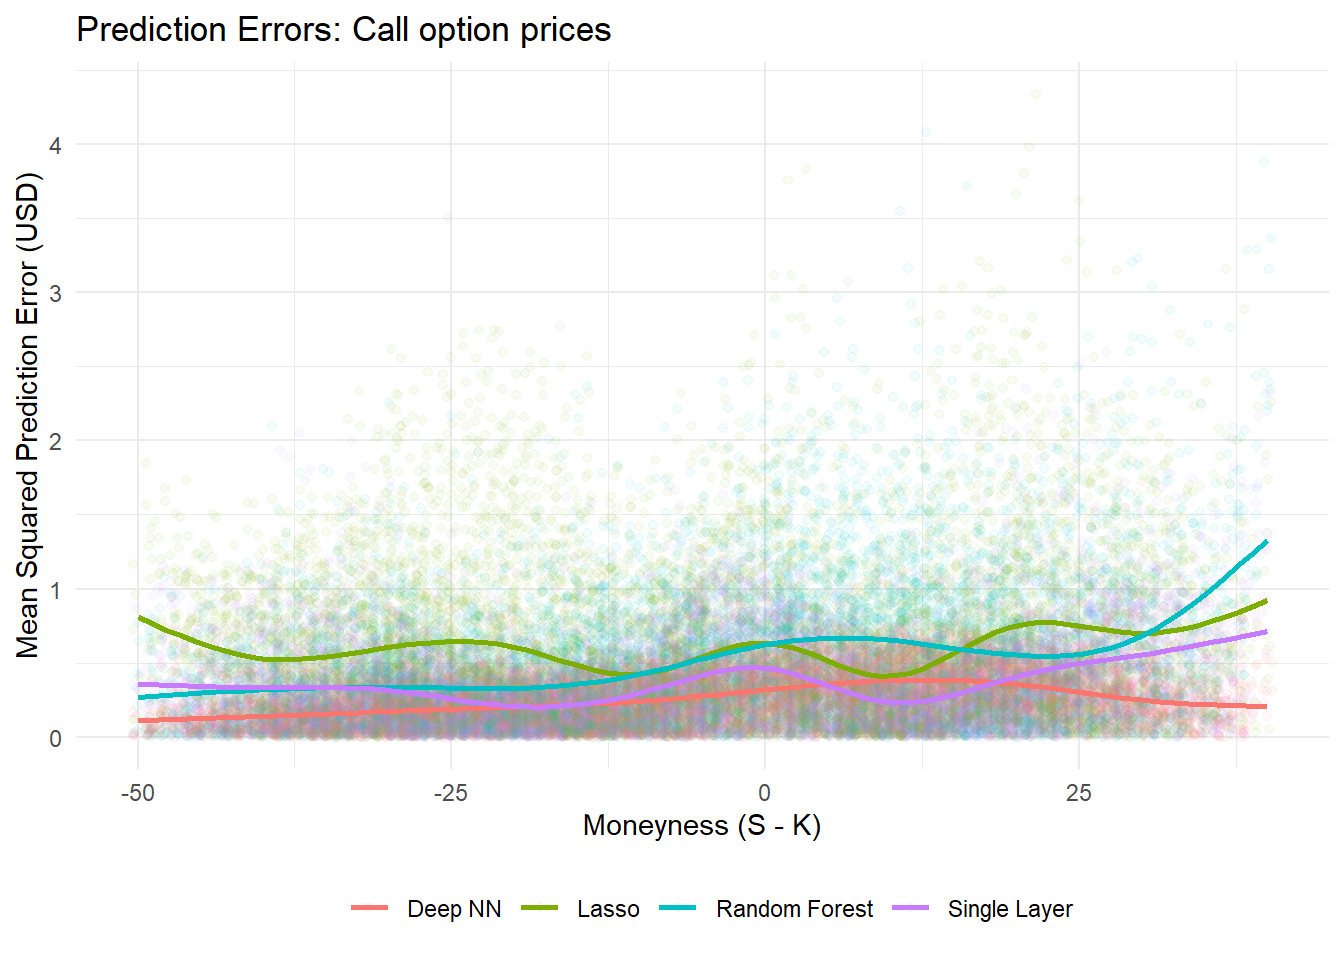
\includegraphics{41_option_pricing_via_machine_learning_files/figure-latex/unnamed-chunk-14-1} \end{center}

The results can be summarized as follow: i) All ML methods seem to be able to \emph{price} call options after observing the training test set. ii) The average prediction errors increase for far in-the money options, especially for the Single Layer neural network and Random Forests. ii) Random forest and the Lasso seem to perform consistently worse in prediction option prices than the Neural networks. iii) The complexity of the deep neural network relative to the single layer neural network does not result in better out-of-sample predictions.

\hypertarget{exercises-9}{%
\section{Exercises}\label{exercises-9}}

\begin{enumerate}
\def\labelenumi{\arabic{enumi}.}
\tightlist
\item
  Write a function that takes \texttt{y} and a matrix of predictors \texttt{X} as inputs and returns a characterization of the relevant parameters of a regression tree with \textbf{1} branch.
\item
  Create a function that creates predictions for a new matrix of predictors `newX´ based on the estimated regression tree.
\item
  Use the package \texttt{rpart} to \emph{grow} a tree based on the training data and use the illustration tools in \texttt{rpart} to understand which characteristics the tree deems relevant for option pricing.
\item
  Make use of a training and a test set to choose the optimal depth (number of sample splits) of the tree.
\item
  Use `keras' to initialize a sequential neural network that can take the predictors from the training dataset as input, contains at least one hidden layer, and generates continuous predictions. \emph{This sounds harder than it is: }see a simple \href{https://tensorflow.rstudio.com/tutorials/beginners/basic-ml/tutorial_basic_regression/}{regression example here}. How many parameters does the neural network you aim to fit have?
\item
  Next, compile the object. It is important that you specify a loss function. Illustrate the difference in predictive accuracy for different architecture choices.
\end{enumerate}

\hypertarget{part-portfolio-optimization}{%
\part*{Portfolio optimization}\label{part-portfolio-optimization}}


\hypertarget{parametric-portfolio-policies}{%
\chapter{Parametric portfolio policies}\label{parametric-portfolio-policies}}

In this chapter, we introduce different portfolio performance measures to evaluate and compare portfolio allocation strategies.
For this purpose, we introduce a direct way to estimate optimal portfolio weights for large-scale cross-sectional applications. More precisely, the approach of \citet{Brandt2009} proposes to parametrize the optimal portfolio weights as a function of stock characteristics directly, instead of estimating the stock's expected return, variance, and covariances with other stocks in a prior step.
We chose weights as a function of the characteristics which maximize the expected utility of the investor. This approach is feasible for large portfolio dimensions (such as the entire CRSP universe) and has been proposed by \citet{Brandt2009}. The review paper \citet{Brandt2010} provides an excellent treatment of related portfolio choice methods.

\hypertarget{data-preparation-6}{%
\section{Data preparation}\label{data-preparation-6}}

To get started, we load the required packages alongside the monthly CRSP file, which forms our investment universe. We load the data from our \texttt{SQLite}-database introduced in our chapter on \emph{``Accessing \& managing financial data''}.

\begin{Shaded}
\begin{Highlighting}[]
\FunctionTok{library}\NormalTok{(tidyverse)}
\FunctionTok{library}\NormalTok{(lubridate)}
\FunctionTok{library}\NormalTok{(RSQLite)}
\end{Highlighting}
\end{Shaded}

\begin{Shaded}
\begin{Highlighting}[]
\NormalTok{tidy\_finance }\OtherTok{\textless{}{-}} \FunctionTok{dbConnect}\NormalTok{(}
  \FunctionTok{SQLite}\NormalTok{(), }\StringTok{"data/tidy\_finance.sqlite"}\NormalTok{, }\AttributeTok{extended\_types =} \ConstantTok{TRUE}
\NormalTok{)}

\NormalTok{crsp\_monthly }\OtherTok{\textless{}{-}} \FunctionTok{tbl}\NormalTok{(tidy\_finance, }\StringTok{"crsp\_monthly"}\NormalTok{) }\SpecialCharTok{|}\ErrorTok{\textgreater{}}
  \FunctionTok{collect}\NormalTok{()}
\end{Highlighting}
\end{Shaded}

To evaluate the performance of portfolios, we further use monthly market returns as a benchmark to compute CAPM alphas.

\begin{Shaded}
\begin{Highlighting}[]
\NormalTok{factors\_ff\_monthly }\OtherTok{\textless{}{-}} \FunctionTok{tbl}\NormalTok{(tidy\_finance, }\StringTok{"factors\_ff\_monthly"}\NormalTok{) }\SpecialCharTok{|}\ErrorTok{\textgreater{}}
  \FunctionTok{collect}\NormalTok{()}
\end{Highlighting}
\end{Shaded}

Next, we retrieve some stock characteristics that have been shown to have an effect on the expected returns or expected variances (or even higher moments) of the return distribution. In particular, we record the lagged one-year return momentum (\texttt{momentum\_lag}), defined as the compounded return between months \(t − 13\) and \(t − 2\) for each firm. The second characteristic is the firm's market equity (\texttt{size\_lag}), defined as the log of the price per share times the number of shares outstanding. To construct the correct lagged values, we use the approach introduced in the chapter on \emph{``Accessing \& managing financial data''}.

\begin{Shaded}
\begin{Highlighting}[]
\NormalTok{crsp\_monthly\_lags }\OtherTok{\textless{}{-}}\NormalTok{ crsp\_monthly }\SpecialCharTok{|}\ErrorTok{\textgreater{}}
  \FunctionTok{transmute}\NormalTok{(permno,}
    \AttributeTok{month\_12 =}\NormalTok{ month }\SpecialCharTok{\%m+\%} \FunctionTok{months}\NormalTok{(}\DecValTok{12}\NormalTok{),}
\NormalTok{    mktcap}
\NormalTok{  )}

\NormalTok{crsp\_monthly }\OtherTok{\textless{}{-}}\NormalTok{ crsp\_monthly }\SpecialCharTok{|}\ErrorTok{\textgreater{}}
  \FunctionTok{inner\_join}\NormalTok{(crsp\_monthly\_lags,}
    \AttributeTok{by =} \FunctionTok{c}\NormalTok{(}\StringTok{"permno"}\NormalTok{, }\StringTok{"month"} \OtherTok{=} \StringTok{"month\_12"}\NormalTok{),}
    \AttributeTok{suffix =} \FunctionTok{c}\NormalTok{(}\StringTok{""}\NormalTok{, }\StringTok{"\_12"}\NormalTok{)}
\NormalTok{  )}

\NormalTok{data\_portfolios }\OtherTok{\textless{}{-}}\NormalTok{ crsp\_monthly }\SpecialCharTok{|}\ErrorTok{\textgreater{}}
  \FunctionTok{mutate}\NormalTok{(}
    \AttributeTok{momentum\_lag =}\NormalTok{ mktcap\_lag }\SpecialCharTok{/}\NormalTok{ mktcap\_12,}
    \AttributeTok{size\_lag =} \FunctionTok{log}\NormalTok{(mktcap\_lag)}
\NormalTok{  ) }\SpecialCharTok{|}\ErrorTok{\textgreater{}}
  \FunctionTok{drop\_na}\NormalTok{(}\FunctionTok{contains}\NormalTok{(}\StringTok{"lag"}\NormalTok{))}
\end{Highlighting}
\end{Shaded}

\hypertarget{parametric-portfolio-policies-1}{%
\section{Parametric portfolio policies}\label{parametric-portfolio-policies-1}}

The basic idea of parametric portfolio weights is as follows. Suppose that at each date \(t\) we have \(N_t\) stocks in the investment universe, where each stock \(i\) has a return of \(r_{i, t+1}\) and is associated with a vector of firm characteristics \(x_{i, t}\) such as time-series momentum or the market capitalization. The investor's problem is to choose portfolio weights \(w_{i,t}\) to maximize the expected utility of the portfolio return:
\[\begin{aligned}
\max_{w} E_t\left(u(r_{p, t+1})\right) = E_t\left[u\left(\sum\limits_{i=1}^{N_t}w_{i,t}r_{i,t+1}\right)\right]
\end{aligned}\]
where \(u(\cdot)\) denotes the utility function.

Where do the stock characteristics show up? We parameterize the optimal portfolio weights as a function of the stock characteristic \(x_{i,t}\) with the following linear specification for the portfolio weights:
\[w_{i,t} = \bar{w}_{i,t} + \frac{1}{N_t}\theta'\hat{x}_{i,t},\]
where \(\bar{w}_{i,t}\) is a stock's weight in a benchmark portfolio (we use the value-weighted or naive portfolio in the application below), \(\theta\) is a vector of coefficients which we are going to estimate, and \(\hat{x}_{i,t}\) are the characteristics of stock \(i\), cross-sectionally standardized to have zero mean and unit standard deviation.

Intuitively, the portfolio strategy is a form of active portfolio management relative to a performance benchmark. Deviations from the benchmark portfolio are derived from the individual stock characteristics. Note that by construction the weights sum up to one as \(\sum_{i=1}^{N_t}\hat{x}_{i,t} = 0\) due to the standardization. Moreover, the coefficients are constant across assets and over time. The implicit assumption is that the characteristics fully capture all aspects of the joint distribution of returns that are relevant for forming optimal portfolios.

We first implement cross-sectional standardization for the entire CRSP universe. We also keep track of (lagged) relative market capitalization \texttt{relative\_mktcap}, which will represent the value-weighted benchmark portfolio, while \texttt{n} denotes the number of traded assets \(N_t\), which we use to construct the naive portfolio benchmark.

\begin{Shaded}
\begin{Highlighting}[]
\NormalTok{data\_portfolios }\OtherTok{\textless{}{-}}\NormalTok{ data\_portfolios }\SpecialCharTok{|}\ErrorTok{\textgreater{}}
  \FunctionTok{group\_by}\NormalTok{(month) }\SpecialCharTok{|}\ErrorTok{\textgreater{}}
  \FunctionTok{mutate}\NormalTok{(}
    \AttributeTok{n =} \FunctionTok{n}\NormalTok{(),}
    \AttributeTok{relative\_mktcap =}\NormalTok{ mktcap\_lag }\SpecialCharTok{/} \FunctionTok{sum}\NormalTok{(mktcap\_lag),}
    \FunctionTok{across}\NormalTok{(}\FunctionTok{contains}\NormalTok{(}\StringTok{"lag"}\NormalTok{), }\SpecialCharTok{\textasciitilde{}}\NormalTok{ (. }\SpecialCharTok{{-}} \FunctionTok{mean}\NormalTok{(.)) }\SpecialCharTok{/} \FunctionTok{sd}\NormalTok{(.)),}
\NormalTok{  ) }\SpecialCharTok{|}\ErrorTok{\textgreater{}}
  \FunctionTok{ungroup}\NormalTok{() }\SpecialCharTok{|}\ErrorTok{\textgreater{}}
  \FunctionTok{select}\NormalTok{(}\SpecialCharTok{{-}}\NormalTok{mktcap\_lag, }\SpecialCharTok{{-}}\NormalTok{altprc)}
\end{Highlighting}
\end{Shaded}

\hypertarget{computing-portfolio-weights}{%
\section{Computing portfolio weights}\label{computing-portfolio-weights}}

Next, we move to identify optimal choices of \(\theta\). We rewrite the optimization problem together with the weight parametrization and can then estimate \(\theta\) to maximize the objective function based on our sample
\[\begin{aligned}
E_t\left(u(r_{p, t+1})\right) = \frac{1}{T}\sum\limits_{t=0}^{T-1}u\left(\sum\limits_{i=1}^{N_t}\left(\bar{w}_{i,t} + \frac{1}{N_t}\theta'\hat{x}_{i,t}\right)r_{i,t+1}\right).
\end{aligned}\]
The allocation strategy is straightforward because the number of parameters to estimate is small. Instead of a tedious specification of the \(N_t\) dimensional vector of expected returns and the \(N_t(N_t+1)/2\) free elements of the covariance matrix, all we need to focus on in our application is the vector \(\theta\). \(\theta\) contains only two elements in our application - the relative deviation from the benchmark due to \emph{size} and \emph{momentum}.

To get a feeling for the performance of such an allocation strategy, we start with an arbitrary initial vector \(\theta_0\). The next step is to choose \(\theta\) optimally to maximize the objective function. We automatically detect the number of parameters by counting the number of columns with lagged values.

\begin{Shaded}
\begin{Highlighting}[]
\NormalTok{n\_parameters }\OtherTok{\textless{}{-}} \FunctionTok{sum}\NormalTok{(}\FunctionTok{grepl}\NormalTok{(}
  \StringTok{"lag"}\NormalTok{,}
  \FunctionTok{colnames}\NormalTok{(data\_portfolios)}
\NormalTok{))}
\NormalTok{theta }\OtherTok{\textless{}{-}} \FunctionTok{rep}\NormalTok{(}\FloatTok{1.5}\NormalTok{, n\_parameters)}
\FunctionTok{names}\NormalTok{(theta) }\OtherTok{\textless{}{-}} \FunctionTok{colnames}\NormalTok{(data\_portfolios)[}\FunctionTok{grepl}\NormalTok{(}
  \StringTok{"lag"}\NormalTok{,}
  \FunctionTok{colnames}\NormalTok{(data\_portfolios)}
\NormalTok{)]}
\end{Highlighting}
\end{Shaded}

The function \texttt{compute\_portfolio\_weights} below computes the portfolio weights \(\bar{w}_{i,t} + \frac{1}{N_t}\theta'\hat{x}_{i,t}\) according to our parametrization for a given value \(\theta_0\) of \(\theta\). Everything happens within a single pipeline, hence we provide a short walkthrough.

We first compute \texttt{characteristic\_tilt}, the tilting values \(\frac{1}{N_t}\theta'\hat{x}_{i, t}\) which resemble the deviation from the benchmark portfolio. Next, we compute the benchmark portfolio \texttt{weight\_benchmark}, which can be any reasonable set of portfolio weights. In our case, we choose either the value or equal-weighted allocation.
\texttt{weight\_tilt} completes the picture and contains the final portfolio weights \texttt{weight\_tilt\ =\ weight\_benchmark\ +\ characteristic\_tilt} which deviate from the benchmark portfolio depending on the stock characteristics.

The final few lines go a bit further and implement a simple version of a no-short sale constraint. While it is generally not straightforward to ensure portfolio weight constraints via the parameterization, we simply normalize the portfolio weights such that they are enforced to be positive. Finally, we make sure that the normalized weights sum up to one again. We do so by\\
\[w_{i,t}^+ = \frac{\max(0, w_{i,t})}{\sum\limits_{j=1}^{N_t}\max(0, w_{i,t})}.\]

The following function computes the optimal portfolio weights in the way just described.

\begin{Shaded}
\begin{Highlighting}[]
\NormalTok{compute\_portfolio\_weights }\OtherTok{\textless{}{-}} \ControlFlowTok{function}\NormalTok{(theta,}
\NormalTok{                                      data,}
                                      \AttributeTok{value\_weighting =} \ConstantTok{TRUE}\NormalTok{,}
                                      \AttributeTok{allow\_short\_selling =} \ConstantTok{TRUE}\NormalTok{) \{}
\NormalTok{  data }\SpecialCharTok{|}\ErrorTok{\textgreater{}}
    \FunctionTok{group\_by}\NormalTok{(month) }\SpecialCharTok{|}\ErrorTok{\textgreater{}}
    \FunctionTok{bind\_cols}\NormalTok{(}
      \AttributeTok{characteristic\_tilt =}\NormalTok{ data }\SpecialCharTok{|}\ErrorTok{\textgreater{}}
        \FunctionTok{transmute}\NormalTok{(}\FunctionTok{across}\NormalTok{(}\FunctionTok{contains}\NormalTok{(}\StringTok{"lag"}\NormalTok{), }\SpecialCharTok{\textasciitilde{}}\NormalTok{ . }\SpecialCharTok{/}\NormalTok{ n)) }\SpecialCharTok{|}\ErrorTok{\textgreater{}}
        \FunctionTok{as.matrix}\NormalTok{() }\SpecialCharTok{\%*\%}\NormalTok{ theta }\SpecialCharTok{|}\ErrorTok{\textgreater{}} \FunctionTok{as.numeric}\NormalTok{()}
\NormalTok{    ) }\SpecialCharTok{|}\ErrorTok{\textgreater{}}
    \FunctionTok{mutate}\NormalTok{(}
      \CommentTok{\# Definition of benchmark weight}
      \AttributeTok{weight\_benchmark =} \FunctionTok{case\_when}\NormalTok{(}
\NormalTok{        value\_weighting }\SpecialCharTok{==} \ConstantTok{TRUE} \SpecialCharTok{\textasciitilde{}}\NormalTok{ relative\_mktcap,}
\NormalTok{        value\_weighting }\SpecialCharTok{==} \ConstantTok{FALSE} \SpecialCharTok{\textasciitilde{}} \DecValTok{1} \SpecialCharTok{/}\NormalTok{ n}
\NormalTok{      ),}
      \CommentTok{\# Parametric portfolio weights}
      \AttributeTok{weight\_tilt =}\NormalTok{ weight\_benchmark }\SpecialCharTok{+}\NormalTok{ characteristic\_tilt,}
      \CommentTok{\# Short{-}sell constraint}
      \AttributeTok{weight\_tilt =} \FunctionTok{case\_when}\NormalTok{(}
\NormalTok{        allow\_short\_selling }\SpecialCharTok{==} \ConstantTok{TRUE} \SpecialCharTok{\textasciitilde{}}\NormalTok{ weight\_tilt,}
\NormalTok{        allow\_short\_selling }\SpecialCharTok{==} \ConstantTok{FALSE} \SpecialCharTok{\textasciitilde{}} \FunctionTok{pmax}\NormalTok{(}\DecValTok{0}\NormalTok{, weight\_tilt)}
\NormalTok{      ),}
      \CommentTok{\# Weights sum up to 1}
      \AttributeTok{weight\_tilt =}\NormalTok{ weight\_tilt }\SpecialCharTok{/} \FunctionTok{sum}\NormalTok{(weight\_tilt)}
\NormalTok{    ) }\SpecialCharTok{|}\ErrorTok{\textgreater{}}
    \FunctionTok{ungroup}\NormalTok{()}
\NormalTok{\}}
\end{Highlighting}
\end{Shaded}

In the next step we compute the portfolio weights for the arbitrary vector \(\theta_0\). In the example below, we use the value-weighted portfolio as a benchmark and allow negative portfolio weights.

\begin{Shaded}
\begin{Highlighting}[]
\NormalTok{weights\_crsp }\OtherTok{\textless{}{-}} \FunctionTok{compute\_portfolio\_weights}\NormalTok{(theta,}
\NormalTok{  data\_portfolios,}
  \AttributeTok{value\_weighting =} \ConstantTok{TRUE}\NormalTok{,}
  \AttributeTok{allow\_short\_selling =} \ConstantTok{TRUE}
\NormalTok{)}
\end{Highlighting}
\end{Shaded}

\hypertarget{portfolio-performance}{%
\section{Portfolio performance}\label{portfolio-performance}}

Are the computed weights optimal in any way? Most likely not, as we picked \(\theta_0\) arbitrarily. To evaluate the performance of an allocation strategy, one can think of many different approaches. In their original paper, \citet{Brandt2009} focus on a simple evaluation of the hypothetical utility of an agent equipped with a power utility function \(u_\gamma(r) = \frac{(1 + r)^\gamma}{1-\gamma}\), where \(\gamma\) is the risk aversion factor.

\begin{Shaded}
\begin{Highlighting}[]
\NormalTok{power\_utility }\OtherTok{\textless{}{-}} \ControlFlowTok{function}\NormalTok{(r, }\AttributeTok{gamma =} \DecValTok{5}\NormalTok{) \{}
\NormalTok{  (}\DecValTok{1} \SpecialCharTok{+}\NormalTok{ r)}\SpecialCharTok{\^{}}\NormalTok{(}\DecValTok{1} \SpecialCharTok{{-}}\NormalTok{ gamma) }\SpecialCharTok{/}\NormalTok{ (}\DecValTok{1} \SpecialCharTok{{-}}\NormalTok{ gamma)}
\NormalTok{\}}
\end{Highlighting}
\end{Shaded}

It should be noted, that \citet{Gehrig2020} warn that in the leading case of constant relative risk aversion (CRRA) strong assumptions on the properties of the returns, the variables used to implement the parametric portfolio policy and the
parameter space are necessary to obtain a well defined optimization problem.

No doubt, there are many other ways to evaluate a portfolio. The function below provides a summary of all kinds of interesting measures that can be considered relevant. Do we need all these evaluation measures? It depends: The original paper \citet{Brandt2009} only cares about expected utility to choose \(\theta\). However, if you want to choose optimal values that achieve the highest performance while putting some constraints on your portfolio weights, it is helpful to have everything in one function.

\begin{Shaded}
\begin{Highlighting}[]
\NormalTok{evaluate\_portfolio }\OtherTok{\textless{}{-}} \ControlFlowTok{function}\NormalTok{(weights\_crsp,}
                               \AttributeTok{full\_evaluation =} \ConstantTok{TRUE}\NormalTok{) \{}
\NormalTok{  evaluation }\OtherTok{\textless{}{-}}\NormalTok{ weights\_crsp }\SpecialCharTok{|}\ErrorTok{\textgreater{}}
    \FunctionTok{group\_by}\NormalTok{(month) }\SpecialCharTok{|}\ErrorTok{\textgreater{}}
    \FunctionTok{summarize}\NormalTok{(}
      \AttributeTok{return\_tilt =} \FunctionTok{weighted.mean}\NormalTok{(ret\_excess, weight\_tilt),}
      \AttributeTok{return\_benchmark =} \FunctionTok{weighted.mean}\NormalTok{(ret\_excess, weight\_benchmark)}
\NormalTok{    ) }\SpecialCharTok{|}\ErrorTok{\textgreater{}}
    \FunctionTok{pivot\_longer}\NormalTok{(}\SpecialCharTok{{-}}\NormalTok{month,}
      \AttributeTok{values\_to =} \StringTok{"portfolio\_return"}\NormalTok{,}
      \AttributeTok{names\_to =} \StringTok{"model"}
\NormalTok{    ) }\SpecialCharTok{|}\ErrorTok{\textgreater{}}
    \FunctionTok{group\_by}\NormalTok{(model) }\SpecialCharTok{|}\ErrorTok{\textgreater{}}
    \FunctionTok{left\_join}\NormalTok{(factors\_ff\_monthly, }\AttributeTok{by =} \StringTok{"month"}\NormalTok{) }\SpecialCharTok{|}\ErrorTok{\textgreater{}}
    \FunctionTok{summarize}\NormalTok{(}\FunctionTok{tibble}\NormalTok{(}
      \StringTok{"Expected utility"} \OtherTok{=} \FunctionTok{mean}\NormalTok{(}\FunctionTok{power\_utility}\NormalTok{(portfolio\_return)),}
      \StringTok{"Average return"} \OtherTok{=} \DecValTok{100} \SpecialCharTok{*} \FunctionTok{mean}\NormalTok{(}\DecValTok{12} \SpecialCharTok{*}\NormalTok{ portfolio\_return),}
      \StringTok{"SD return"} \OtherTok{=} \DecValTok{100} \SpecialCharTok{*} \FunctionTok{sqrt}\NormalTok{(}\DecValTok{12}\NormalTok{) }\SpecialCharTok{*} \FunctionTok{sd}\NormalTok{(portfolio\_return),}
      \StringTok{"Sharpe ratio"} \OtherTok{=} \FunctionTok{mean}\NormalTok{(portfolio\_return) }\SpecialCharTok{/} \FunctionTok{sd}\NormalTok{(portfolio\_return),}
      \StringTok{"CAPM alpha"} \OtherTok{=} \FunctionTok{coefficients}\NormalTok{(}\FunctionTok{lm}\NormalTok{(portfolio\_return }\SpecialCharTok{\textasciitilde{}}\NormalTok{ mkt\_excess))[}\DecValTok{1}\NormalTok{],}
      \StringTok{"Market beta"} \OtherTok{=} \FunctionTok{coefficients}\NormalTok{(}\FunctionTok{lm}\NormalTok{(portfolio\_return }\SpecialCharTok{\textasciitilde{}}\NormalTok{ mkt\_excess))[}\DecValTok{2}\NormalTok{]}
\NormalTok{    )) }\SpecialCharTok{|}\ErrorTok{\textgreater{}}
    \FunctionTok{mutate}\NormalTok{(}\AttributeTok{model =} \FunctionTok{gsub}\NormalTok{(}\StringTok{"return\_"}\NormalTok{, }\StringTok{""}\NormalTok{, model)) }\SpecialCharTok{|}\ErrorTok{\textgreater{}}
    \FunctionTok{pivot\_longer}\NormalTok{(}\SpecialCharTok{{-}}\NormalTok{model, }\AttributeTok{names\_to =} \StringTok{"measure"}\NormalTok{) }\SpecialCharTok{|}\ErrorTok{\textgreater{}}
    \FunctionTok{pivot\_wider}\NormalTok{(}\AttributeTok{names\_from =}\NormalTok{ model, }\AttributeTok{values\_from =}\NormalTok{ value)}

  \ControlFlowTok{if}\NormalTok{ (full\_evaluation) \{}
\NormalTok{    weight\_evaluation }\OtherTok{\textless{}{-}}\NormalTok{ weights\_crsp }\SpecialCharTok{|}\ErrorTok{\textgreater{}}
      \FunctionTok{select}\NormalTok{(month, }\FunctionTok{contains}\NormalTok{(}\StringTok{"weight"}\NormalTok{)) }\SpecialCharTok{|}\ErrorTok{\textgreater{}}
      \FunctionTok{pivot\_longer}\NormalTok{(}\SpecialCharTok{{-}}\NormalTok{month, }\AttributeTok{values\_to =} \StringTok{"weight"}\NormalTok{, }\AttributeTok{names\_to =} \StringTok{"model"}\NormalTok{) }\SpecialCharTok{|}\ErrorTok{\textgreater{}}
      \FunctionTok{group\_by}\NormalTok{(model, month) }\SpecialCharTok{|}\ErrorTok{\textgreater{}}
      \FunctionTok{transmute}\NormalTok{(}\FunctionTok{tibble}\NormalTok{(}
        \StringTok{"Absolute weight"} \OtherTok{=} \FunctionTok{abs}\NormalTok{(weight),}
        \StringTok{"Max. weight"} \OtherTok{=} \FunctionTok{max}\NormalTok{(weight),}
        \StringTok{"Min. weight"} \OtherTok{=} \FunctionTok{min}\NormalTok{(weight),}
        \StringTok{"Avg. sum of negative weights"} \OtherTok{=} \SpecialCharTok{{-}}\FunctionTok{sum}\NormalTok{(weight[weight }\SpecialCharTok{\textless{}} \DecValTok{0}\NormalTok{]),}
        \StringTok{"Avg. fraction of negative weights"} \OtherTok{=} \FunctionTok{sum}\NormalTok{(weight }\SpecialCharTok{\textless{}} \DecValTok{0}\NormalTok{) }\SpecialCharTok{/} \FunctionTok{n}\NormalTok{()}
\NormalTok{      )) }\SpecialCharTok{|}\ErrorTok{\textgreater{}}
      \FunctionTok{group\_by}\NormalTok{(model) }\SpecialCharTok{|}\ErrorTok{\textgreater{}}
      \FunctionTok{summarize}\NormalTok{(}\FunctionTok{across}\NormalTok{(}\SpecialCharTok{{-}}\NormalTok{month, }\SpecialCharTok{\textasciitilde{}} \DecValTok{100} \SpecialCharTok{*} \FunctionTok{mean}\NormalTok{(.))) }\SpecialCharTok{|}\ErrorTok{\textgreater{}}
      \FunctionTok{mutate}\NormalTok{(}\AttributeTok{model =} \FunctionTok{gsub}\NormalTok{(}\StringTok{"weight\_"}\NormalTok{, }\StringTok{""}\NormalTok{, model)) }\SpecialCharTok{|}\ErrorTok{\textgreater{}}
      \FunctionTok{pivot\_longer}\NormalTok{(}\SpecialCharTok{{-}}\NormalTok{model, }\AttributeTok{names\_to =} \StringTok{"measure"}\NormalTok{) }\SpecialCharTok{|}\ErrorTok{\textgreater{}}
      \FunctionTok{pivot\_wider}\NormalTok{(}\AttributeTok{names\_from =}\NormalTok{ model, }\AttributeTok{values\_from =}\NormalTok{ value)}
\NormalTok{    evaluation }\OtherTok{\textless{}{-}} \FunctionTok{bind\_rows}\NormalTok{(evaluation, weight\_evaluation)}
\NormalTok{  \}}
  \FunctionTok{return}\NormalTok{(evaluation)}
\NormalTok{\}}
\end{Highlighting}
\end{Shaded}

Let us take a look at the different portfolio strategies and evaluation measures.

\begin{Shaded}
\begin{Highlighting}[]
\FunctionTok{evaluate\_portfolio}\NormalTok{(weights\_crsp) }\SpecialCharTok{|}\ErrorTok{\textgreater{}} 
  \FunctionTok{print}\NormalTok{(}\AttributeTok{n =} \ConstantTok{Inf}\NormalTok{)}
\end{Highlighting}
\end{Shaded}

\begin{verbatim}
## # A tibble: 11 x 3
##    measure                           benchmark     tilt
##    <chr>                                 <dbl>    <dbl>
##  1 Expected utility                   -2.49e-1 -0.262  
##  2 Average return                      6.86e+0 -0.604  
##  3 SD return                           1.53e+1 21.0    
##  4 Sharpe ratio                        1.29e-1 -0.00831
##  5 CAPM alpha                          1.08e-4 -0.00574
##  6 Market beta                         9.92e-1  0.927  
##  7 Absolute weight                     2.46e-2  0.0631 
##  8 Max. weight                         3.52e+0  3.65   
##  9 Min. weight                         2.78e-5 -0.145  
## 10 Avg. sum of negative weights        0       78.0    
## 11 Avg. fraction of negative weights   0       49.4
\end{verbatim}

The value-weighted portfolio delivers an annualized return of more than 6 percent and clearly outperforms the tilted portfolio, irrespective of whether we evaluate expected utility, the Sharpe ratio or the CAPM alpha. We can conclude the market beta is close to one for both strategies (naturally almost identically 1 for the value-weighted benchmark portfolio). When it comes to the distribution of the portfolio weights, we see that the benchmark portfolio weight takes less extreme positions (lower average absolute weights and lower maximum weight). By definition, the value-weighted benchmark does not take any negative positions, while the tilted portfolio also takes short positions.

\hypertarget{optimal-parameter-choice}{%
\section{Optimal parameter choice}\label{optimal-parameter-choice}}

Next, we move to a choice of \(\theta\) that actually aims to improve some (or all) of the performance measures. We first define a helper function \texttt{compute\_objective\_function}, which we then pass to an optimizer.

\begin{Shaded}
\begin{Highlighting}[]
\NormalTok{compute\_objective\_function }\OtherTok{\textless{}{-}} \ControlFlowTok{function}\NormalTok{(theta,}
\NormalTok{                                       data,}
                                       \AttributeTok{objective\_measure =} \StringTok{"Expected utility"}\NormalTok{,}
                                       \AttributeTok{value\_weighting =} \ConstantTok{TRUE}\NormalTok{,}
                                       \AttributeTok{allow\_short\_selling =} \ConstantTok{TRUE}\NormalTok{) \{}
\NormalTok{  processed\_data }\OtherTok{\textless{}{-}} \FunctionTok{compute\_portfolio\_weights}\NormalTok{(}
\NormalTok{    theta,}
\NormalTok{    data,}
\NormalTok{    value\_weighting,}
\NormalTok{    allow\_short\_selling}
\NormalTok{  )}

\NormalTok{  objective\_function }\OtherTok{\textless{}{-}} \FunctionTok{evaluate\_portfolio}\NormalTok{(processed\_data,}
    \AttributeTok{full\_evaluation =} \ConstantTok{FALSE}
\NormalTok{  ) }\SpecialCharTok{|}\ErrorTok{\textgreater{}}
    \FunctionTok{filter}\NormalTok{(measure }\SpecialCharTok{==}\NormalTok{ objective\_measure) }\SpecialCharTok{|}\ErrorTok{\textgreater{}}
    \FunctionTok{pull}\NormalTok{(tilt)}

  \FunctionTok{return}\NormalTok{(}\SpecialCharTok{{-}}\NormalTok{objective\_function)}
\NormalTok{\}}
\end{Highlighting}
\end{Shaded}

You may wonder why we return the negative value of the objective function. This is simply due to the common convention for optimization procedures to search for minima as a default. By minimizing the negative value of the objective function, we get the maximum value as a result.
In its most basic form, R optimization relies on the function \texttt{optim}. As main inputs, the function requires an initial guess of the parameters and the objective function to minimize. Now, we are fully equipped to compute the optimal values of \(\hat\theta\), which maximize the hypothetical expected utility of the investor.

\begin{Shaded}
\begin{Highlighting}[]
\NormalTok{optimal\_theta }\OtherTok{\textless{}{-}} \FunctionTok{optim}\NormalTok{(}
  \AttributeTok{par =}\NormalTok{ theta,}
\NormalTok{  compute\_objective\_function,}
  \AttributeTok{objective\_measure =} \StringTok{"Expected utility"}\NormalTok{,}
  \AttributeTok{data =}\NormalTok{ data\_portfolios,}
  \AttributeTok{value\_weighting =} \ConstantTok{TRUE}\NormalTok{,}
  \AttributeTok{allow\_short\_selling =} \ConstantTok{TRUE}
\NormalTok{)}

\NormalTok{optimal\_theta}\SpecialCharTok{$}\NormalTok{par}
\end{Highlighting}
\end{Shaded}

\begin{verbatim}
## momentum_lag     size_lag 
##        0.189       -2.007
\end{verbatim}

The resulting values of \(\hat\theta\) are easy to interpret intuitively. Expected utility increases by tilting weights from the value-weighted portfolio towards smaller stocks (negative coefficient for size) and towards past winners (positive value for momentum).

\hypertarget{more-model-specifications}{%
\section{More model specifications}\label{more-model-specifications}}

How does the portfolio perform for different model specifications? For this purpose, we compute the performance of a number of different modeling choices based on the entire CRSP sample. The next code chunk performs all the heavy lifting.

\begin{Shaded}
\begin{Highlighting}[]
\NormalTok{full\_model\_grid }\OtherTok{\textless{}{-}} \FunctionTok{expand\_grid}\NormalTok{(}
  \AttributeTok{value\_weighting =} \FunctionTok{c}\NormalTok{(}\ConstantTok{TRUE}\NormalTok{, }\ConstantTok{FALSE}\NormalTok{),}
  \AttributeTok{allow\_short\_selling =} \FunctionTok{c}\NormalTok{(}\ConstantTok{TRUE}\NormalTok{, }\ConstantTok{FALSE}\NormalTok{),}
  \AttributeTok{data =} \FunctionTok{list}\NormalTok{(data\_portfolios)}
\NormalTok{) }\SpecialCharTok{|}\ErrorTok{\textgreater{}}
  \FunctionTok{mutate}\NormalTok{(}\AttributeTok{optimal\_theta =} \FunctionTok{pmap}\NormalTok{(}
    \AttributeTok{.l =} \FunctionTok{list}\NormalTok{(}
\NormalTok{      data,}
\NormalTok{      value\_weighting,}
\NormalTok{      allow\_short\_selling}
\NormalTok{    ),}
    \AttributeTok{.f =} \SpecialCharTok{\textasciitilde{}} \FunctionTok{optim}\NormalTok{(}
      \AttributeTok{par =}\NormalTok{ theta,}
\NormalTok{      compute\_objective\_function,}
      \AttributeTok{data =}\NormalTok{ ..}\DecValTok{1}\NormalTok{,}
      \AttributeTok{objective\_measure =} \StringTok{"Expected utility"}\NormalTok{,}
      \AttributeTok{value\_weighting =}\NormalTok{ ..}\DecValTok{2}\NormalTok{,}
      \AttributeTok{allow\_short\_selling =}\NormalTok{ ..}\DecValTok{3}
\NormalTok{    )}\SpecialCharTok{$}\NormalTok{par}
\NormalTok{  ))}
\end{Highlighting}
\end{Shaded}

Finally, we can compare the results. The table below shows summary statistics for all possible combinations: equal- or value-weighted benchmark portfolio, with or without short-selling constraints, and tilted towards maximizing expected utility.

\begin{Shaded}
\begin{Highlighting}[]
\NormalTok{performance\_table }\OtherTok{\textless{}{-}}\NormalTok{ full\_model\_grid }\SpecialCharTok{|}\ErrorTok{\textgreater{}}
  \FunctionTok{mutate}\NormalTok{(}
    \AttributeTok{processed\_data =} \FunctionTok{pmap}\NormalTok{(}
      \AttributeTok{.l =} \FunctionTok{list}\NormalTok{(}
\NormalTok{        optimal\_theta,}
\NormalTok{        data,}
\NormalTok{        value\_weighting,}
\NormalTok{        allow\_short\_selling}
\NormalTok{      ),}
      \AttributeTok{.f =} \SpecialCharTok{\textasciitilde{}} \FunctionTok{compute\_portfolio\_weights}\NormalTok{(..}\DecValTok{1}\NormalTok{, ..}\DecValTok{2}\NormalTok{, ..}\DecValTok{3}\NormalTok{, ..}\DecValTok{4}\NormalTok{)}
\NormalTok{    ),}
    \AttributeTok{portfolio\_evaluation =} \FunctionTok{map}\NormalTok{(processed\_data,}
\NormalTok{      evaluate\_portfolio,}
      \AttributeTok{full\_evaluation =} \ConstantTok{TRUE}
\NormalTok{    )}
\NormalTok{  ) }\SpecialCharTok{|}\ErrorTok{\textgreater{}}
  \FunctionTok{select}\NormalTok{(}
\NormalTok{    value\_weighting,}
\NormalTok{    allow\_short\_selling,}
\NormalTok{    portfolio\_evaluation}
\NormalTok{  ) }\SpecialCharTok{|}\ErrorTok{\textgreater{}}
  \FunctionTok{unnest}\NormalTok{(portfolio\_evaluation)}

\NormalTok{performance\_table }\SpecialCharTok{|}\ErrorTok{\textgreater{}}
  \FunctionTok{rename}\NormalTok{(}
    \StringTok{" "} \OtherTok{=}\NormalTok{ benchmark,}
    \AttributeTok{Optimal =}\NormalTok{ tilt}
\NormalTok{  ) }\SpecialCharTok{|}\ErrorTok{\textgreater{}}
  \FunctionTok{mutate}\NormalTok{(}
    \AttributeTok{value\_weighting =} \FunctionTok{case\_when}\NormalTok{(}
\NormalTok{      value\_weighting }\SpecialCharTok{==} \ConstantTok{TRUE} \SpecialCharTok{\textasciitilde{}} \StringTok{"VW"}\NormalTok{,}
\NormalTok{      value\_weighting }\SpecialCharTok{==} \ConstantTok{FALSE} \SpecialCharTok{\textasciitilde{}} \StringTok{"EW"}
\NormalTok{    ),}
    \AttributeTok{allow\_short\_selling =} \FunctionTok{case\_when}\NormalTok{(}
\NormalTok{      allow\_short\_selling }\SpecialCharTok{==} \ConstantTok{TRUE} \SpecialCharTok{\textasciitilde{}} \StringTok{""}\NormalTok{,}
\NormalTok{      allow\_short\_selling }\SpecialCharTok{==} \ConstantTok{FALSE} \SpecialCharTok{\textasciitilde{}} \StringTok{"(no s.)"}
\NormalTok{    )}
\NormalTok{  ) }\SpecialCharTok{|}\ErrorTok{\textgreater{}}
  \FunctionTok{pivot\_wider}\NormalTok{(}
    \AttributeTok{names\_from =}\NormalTok{ value\_weighting}\SpecialCharTok{:}\NormalTok{allow\_short\_selling,}
    \AttributeTok{values\_from =} \StringTok{" "}\SpecialCharTok{:}\NormalTok{Optimal,}
    \AttributeTok{names\_glue =} \StringTok{"\{value\_weighting\} \{allow\_short\_selling\} \{.value\} "}
\NormalTok{  ) }\SpecialCharTok{|}\ErrorTok{\textgreater{}}
  \FunctionTok{select}\NormalTok{(}
\NormalTok{    measure,}
    \StringTok{\textasciigrave{}}\AttributeTok{EW    }\StringTok{\textasciigrave{}}\NormalTok{,}
    \StringTok{\textasciigrave{}}\AttributeTok{VW    }\StringTok{\textasciigrave{}}\NormalTok{,}
    \FunctionTok{sort}\NormalTok{(}\FunctionTok{contains}\NormalTok{(}\StringTok{"Optimal"}\NormalTok{))}
\NormalTok{  ) }\SpecialCharTok{|}\ErrorTok{\textgreater{}}
  \FunctionTok{print}\NormalTok{(}\AttributeTok{n =} \DecValTok{11}\NormalTok{, }\AttributeTok{max\_extra\_cols =} \DecValTok{7}\NormalTok{)}
\end{Highlighting}
\end{Shaded}

\begin{verbatim}
## # A tibble: 11 x 7
##    measure             `EW    ` `VW    ` `VW  Optimal `
##    <chr>                  <dbl>    <dbl>          <dbl>
##  1 Expected utility    -0.250   -2.49e-1       -0.247  
##  2 Average return      10.5      6.86e+0       14.7    
##  3 SD return           20.3      1.53e+1       20.6    
##  4 Sharpe ratio         0.149    1.29e-1        0.206  
##  5 CAPM alpha           0.00231  1.08e-4        0.00649
##  6 Market beta          1.13     9.92e-1        1.01   
##  7 Absolute weight      0.0246   2.46e-2        0.0379 
##  8 Max. weight          0.0246   3.52e+0        3.34   
##  9 Min. weight          0.0246   2.78e-5       -0.0327 
## 10 Avg. sum of negati~  0        0             27.9    
## 11 Avg. fraction of n~  0        0             38.8    
## # ... with 3 more variables:
## #   `VW (no s.) Optimal ` <dbl>, `EW  Optimal ` <dbl>,
## #   `EW (no s.) Optimal ` <dbl>
\end{verbatim}

The results indicate that the average annualized Sharpe ratio of the equal-weighted portfolio exceeds the Sharpe ratio of the value-weighted benchmark portfolio. Nevertheless, starting with the weighted value portfolio as a benchmark and tilting optimally with respect to momentum and small stocks yields the highest Sharpe ratio across all specifications. Imposing no short-sale constraints does not improve the performance of the portfolios in our application.

\hypertarget{exercises-10}{%
\section{Exercises}\label{exercises-10}}

\begin{enumerate}
\def\labelenumi{\arabic{enumi}.}
\tightlist
\item
  How do the estimated parameters \(\hat\theta\) and the portfolio performance change if your objective is to maximize the Sharpe ratio instead of the hypothetical expected utility?
\item
  The code above is very flexible in the sense that you can easily add new firm characteristics. Construct a new characteristic and evaluate the corresponding coefficient \(\hat\theta_i\).
\item
  Tweak the function \texttt{optimal\_theta}such that you can impose additional performance constraints in order to determine \(\hat\theta\) which maximizes expected utility under the constraint that the market beta is below 1.
\item
  Does the portfolio performance resemble a realistic out-of-sample backtesting procedure? Verify the robustness of the results by first estimating \(\hat\theta\) based on \emph{past data} only. Then, use more recent periods to evaluate the actual portfolio performance.
\item
  By formulating the portfolio problem as a statistical estimation problem, you can easily obtain standard errors for the coefficients of the weight function. \citet{Brandt2009} provide the relevant derivations in their paper in Equation (10). Implement a small function that computes standard errors for \(\hat\theta\).
\end{enumerate}

\hypertarget{constrained-optimization-and-backtesting}{%
\chapter{Constrained optimization and backtesting}\label{constrained-optimization-and-backtesting}}

In this chapter, we conduct portfolio backtesting in a more realistic setting by including transaction costs and investment constraints such as no-short-selling rules. We start with \emph{standard} mean-variance efficient portfolios. Then, we introduce further constraints step-by-step. Numerical constrained optimization is performed by the packages \texttt{quadprog} (for quadratic objective functions such as in typical mean-variance framework) and \texttt{alabama} (for more general, non-linear objectives and constraints).

\begin{Shaded}
\begin{Highlighting}[]
\FunctionTok{library}\NormalTok{(tidyverse)}
\FunctionTok{library}\NormalTok{(RSQLite)}
\FunctionTok{library}\NormalTok{(quadprog)}
\FunctionTok{library}\NormalTok{(alabama)}
\end{Highlighting}
\end{Shaded}

\hypertarget{data-preparation-7}{%
\section{Data preparation}\label{data-preparation-7}}

We start by loading the required data from our \texttt{SQLite}-database introduced in our chapter on \emph{``Accessing \& managing financial data''}. For simplicity, we restrict our investment universe to the monthly Fama-French industry portfolio returns in the following application.

\begin{Shaded}
\begin{Highlighting}[]
\NormalTok{tidy\_finance }\OtherTok{\textless{}{-}} \FunctionTok{dbConnect}\NormalTok{(}\FunctionTok{SQLite}\NormalTok{(), }\StringTok{"data/tidy\_finance.sqlite"}\NormalTok{,}
  \AttributeTok{extended\_types =} \ConstantTok{TRUE}
\NormalTok{)}

\NormalTok{industry\_returns }\OtherTok{\textless{}{-}} \FunctionTok{tbl}\NormalTok{(tidy\_finance, }\StringTok{"industries\_ff\_monthly"}\NormalTok{) }\SpecialCharTok{|}\ErrorTok{\textgreater{}}
  \FunctionTok{collect}\NormalTok{()}

\NormalTok{industry\_returns }\OtherTok{\textless{}{-}}\NormalTok{ industry\_returns }\SpecialCharTok{|}\ErrorTok{\textgreater{}}
  \FunctionTok{select}\NormalTok{(}\SpecialCharTok{{-}}\NormalTok{month)}
\end{Highlighting}
\end{Shaded}

\hypertarget{recap-of-portfolio-choice}{%
\section{Recap of portfolio choice}\label{recap-of-portfolio-choice}}

A common objective for portfolio optimization is to find mean-variance efficient portfolio weights, i.e., the allocation which delivers the lowest possible return variance for a given minimum level of expected returns. In the most extreme case, where the investor is only concerned about portfolio variance, she may choose to implement the minimum variance portfolio (MVP) weights which are given by the solution to
\[w_\text{mvp} = \arg\min w'\Sigma w \text{ s.t. } w'\iota = 1\]
where \(\Sigma\) is the \((N \times N)\) covariance matrix of the returns. The optimal weights \(\omega_\text{mvp}\) can be found analytically and are \(\omega_\text{mvp} = \frac{\Sigma^{-1}\iota}{\iota'\Sigma^{-1}\iota}\). In terms of code, the math is equivalent to the following.

\begin{Shaded}
\begin{Highlighting}[]
\NormalTok{Sigma }\OtherTok{\textless{}{-}} \FunctionTok{cov}\NormalTok{(industry\_returns)}
\NormalTok{w\_mvp }\OtherTok{\textless{}{-}} \FunctionTok{solve}\NormalTok{(Sigma) }\SpecialCharTok{\%*\%} \FunctionTok{rep}\NormalTok{(}\DecValTok{1}\NormalTok{, }\FunctionTok{ncol}\NormalTok{(Sigma))}
\NormalTok{w\_mvp }\OtherTok{\textless{}{-}} \FunctionTok{as.vector}\NormalTok{(w\_mvp }\SpecialCharTok{/} \FunctionTok{sum}\NormalTok{(w\_mvp))}
\end{Highlighting}
\end{Shaded}

Next, consider an investor who aims to achieve minimum variance \emph{given a required expected portfolio return} \(\bar{\mu}\) such that she chooses
\[w_\text{eff}({\bar{\mu}}) =\arg\min w'\Sigma w \text{ s.t. } w'\iota = 1 \text{ and } \omega'\mu \geq \bar{\mu}.\]
It can be shown (see Exercises) that the portfolio choice problem can equivalently be formulated for an investor with mean-variance preferences and risk aversion factor \(\gamma\). The investor aims to choose portfolio weights such that
\[ w^*_\gamma = \arg\max w' \mu - \frac{\gamma}{2}w'\Sigma w\quad s.t. w'\iota = 1.\]
The solution to the optimal portfolio choice problem is:
\[\omega^*_{\gamma}  = \frac{1}{\gamma}\left(\Sigma^{-1} - \frac{1}{\iota' \Sigma^{-1}\iota }\Sigma^{-1}\iota\iota' \Sigma^{-1} \right) \mu  + \frac{1}{\iota' \Sigma^{-1} \iota }\Sigma^{-1} \iota.\]
Empirically, this classical solution imposes many problems. In particular, the estimates of \(\mu_t\) are noisy over short horizons, the (\(N \times N\)) matrix \(\Sigma_t\) contains \(N(N-1)/2\) distinct elements and thus, estimation error is huge. Even worse, if the asset universe contains more assets than available time periods \((N > T)\), the sample covariance matrix is no longer positive definite such that the inverse \(\Sigma^{-1}\) does not exist anymore. On top of the estimation uncertainty, \emph{transaction costs} are a major concern. Rebalancing portfolios is costly, and, therefore, the optimal choice should depend on the investor's current holdings.

\hypertarget{estimation-uncertainty-and-transaction-costs}{%
\section{Estimation uncertainty and transaction costs}\label{estimation-uncertainty-and-transaction-costs}}

The empirical evidence regarding the performance of a mean-variance optimization procedure in which you simply plug in some sample estimates \(\hat \mu_t\) and \(\hat \Sigma_t\) can be summarized rather briefly: mean-variance optimization performs poorly! The literature discusses many proposals to overcome these empirical issues. For instance, one may impose some form of regularization of \(\Sigma\), rely on Bayesian priors inspired by theoretical asset pricing models, or use high-frequency data to improve forecasting. One unifying framework that works easily, effectively (even for large dimensions), and is purely inspired by economic arguments is an ex-ante adjustment for transaction costs \citep{Hautsch2019}.

Assume that returns are from a multivariate normal distribution such that \(p_t({r}_{t+1}|\mathcal{M})=N(\mu,\Sigma)\). Additionally, we assume quadratic transaction costs which penalize rebalancing such that \[
\begin{aligned}
\nu\left(\omega_{t+1},\omega_{t^+}, \beta\right) :=\nu_t\left(\omega_{t+1}, \beta\right) = \frac{\beta}{2} \left(\omega_{t+1} - \omega_{t^+}\right)'\left(\omega_{t+1}- \omega_{t^+}\right),\end{aligned}\]
with cost parameter \(\beta>0\) and \(\omega_{t^+} := {\omega_t \circ (1 +r_{t})}/{\iota' (\omega_t \circ (1 + r_{t}))}\). Note that \(\omega_{t^+}\) differs mechanically from \(\omega_t\) due to the returns in the past period.\\
Then, the optimal portfolio choice is
\[\begin{aligned}\omega_{t+1} ^* &:=  \arg\max_{\omega \in \mathbb{R}^N,  \iota'\omega = 1} \omega'\mu - \nu_t (\omega,\omega_{t^+}, \beta) - \frac{\gamma}{2}\omega'\Sigma\omega \\
&=\arg\max_{\omega\in\mathbb{R}^N,\text{ }  \iota'\omega=1}
\omega'\mu^* - \frac{\gamma}{2}\omega'\Sigma^* \omega ,\end{aligned}\]
where
\[\mu^*:=\mu+\beta \omega_{t^+} \quad  \text{and} \quad \Sigma^*:=\Sigma + \frac{\beta}{\gamma} I_N.\]
As a result, adjusting for transaction costs implies a standard mean-variance optimal portfolio choice with adjusted return parameters \(\Sigma^*\) and \(\mu^*\): \[\omega^*_{t+1} = \frac{1}{\gamma}\left(\Sigma^{*-1} - \frac{1}{\iota' \Sigma^{*-1}\iota }\Sigma^{*-1}\iota\iota' \Sigma^{*-1} \right) \mu^*  + \frac{1}{\iota' \Sigma^{*-1} \iota }\Sigma^{*-1} \iota.\]

An alternative formulation of the optimal portfolio can be derived as follows:
\[\omega_{t+1} ^*=\arg\max_{\omega\in\mathbb{R}^N,\text{ }  \iota'\omega=1}
\omega'\left(\mu+\beta\left(\omega_{t^+} - \frac{1}{N}\iota\right)\right) - \frac{\gamma}{2}\omega'\Sigma^* \omega.\]
The optimal weights correspond to a mean-variance portfolio where the vector of expected returns is such that assets that currently exhibit a higher weight are considered as delivering a higher expected return.

\hypertarget{optimal-portfolio-choice}{%
\section{Optimal portfolio choice}\label{optimal-portfolio-choice}}

The function below implements the efficient portfolio weight in its general form, allowing for transaction costs (conditional on the holdings \emph{before} reallocation). For \(\beta=0\), the computation resembles the standard mean-variance efficient framework. \texttt{gamma} denotes the coefficient of risk aversion,\texttt{beta} is the transaction cost parameter and \texttt{w\_prev} are the weights before rebalancing.

\begin{Shaded}
\begin{Highlighting}[]
\NormalTok{compute\_efficient\_weight }\OtherTok{\textless{}{-}} \ControlFlowTok{function}\NormalTok{(Sigma,}
\NormalTok{                                     mu,}
                                     \AttributeTok{gamma =} \DecValTok{2}\NormalTok{,}
                                     \AttributeTok{beta =} \DecValTok{0}\NormalTok{, }\CommentTok{\# transaction costs}
                                     \AttributeTok{w\_prev =} \DecValTok{1} \SpecialCharTok{/} \FunctionTok{ncol}\NormalTok{(Sigma) }\SpecialCharTok{*} \FunctionTok{rep}\NormalTok{(}\DecValTok{1}\NormalTok{, }\FunctionTok{ncol}\NormalTok{(Sigma))) \{}
\NormalTok{  iota }\OtherTok{\textless{}{-}} \FunctionTok{rep}\NormalTok{(}\DecValTok{1}\NormalTok{, }\FunctionTok{ncol}\NormalTok{(Sigma))}
\NormalTok{  Sigma\_processed }\OtherTok{\textless{}{-}}\NormalTok{ Sigma }\SpecialCharTok{+}\NormalTok{ beta }\SpecialCharTok{/}\NormalTok{ gamma }\SpecialCharTok{*} \FunctionTok{diag}\NormalTok{(}\FunctionTok{ncol}\NormalTok{(Sigma))}
\NormalTok{  mu\_processed }\OtherTok{\textless{}{-}}\NormalTok{ mu }\SpecialCharTok{+}\NormalTok{ beta }\SpecialCharTok{*}\NormalTok{ w\_prev}

\NormalTok{  Sigma\_inverse }\OtherTok{\textless{}{-}} \FunctionTok{solve}\NormalTok{(Sigma\_processed)}

\NormalTok{  w\_mvp }\OtherTok{\textless{}{-}}\NormalTok{ Sigma\_inverse }\SpecialCharTok{\%*\%}\NormalTok{ iota}
\NormalTok{  w\_mvp }\OtherTok{\textless{}{-}} \FunctionTok{as.vector}\NormalTok{(w\_mvp }\SpecialCharTok{/} \FunctionTok{sum}\NormalTok{(w\_mvp))}
\NormalTok{  w\_opt }\OtherTok{\textless{}{-}}\NormalTok{ w\_mvp }\SpecialCharTok{+} \DecValTok{1} \SpecialCharTok{/}\NormalTok{ gamma }\SpecialCharTok{*}
\NormalTok{    (Sigma\_inverse }\SpecialCharTok{{-}} \DecValTok{1} \SpecialCharTok{/} \FunctionTok{sum}\NormalTok{(Sigma\_inverse) }\SpecialCharTok{*}\NormalTok{ Sigma\_inverse }\SpecialCharTok{\%*\%}\NormalTok{ iota }\SpecialCharTok{\%*\%} \FunctionTok{t}\NormalTok{(iota) }\SpecialCharTok{\%*\%}\NormalTok{ Sigma\_inverse) }\SpecialCharTok{\%*\%}
\NormalTok{      mu\_processed}
  \FunctionTok{return}\NormalTok{(}\FunctionTok{as.vector}\NormalTok{(w\_opt))}
\NormalTok{\}}

\NormalTok{mu }\OtherTok{\textless{}{-}} \FunctionTok{colMeans}\NormalTok{(industry\_returns)}
\FunctionTok{compute\_efficient\_weight}\NormalTok{(Sigma, mu)}
\end{Highlighting}
\end{Shaded}

\begin{verbatim}
##  [1]  1.428  0.270 -1.302  0.375  0.308 -0.152  0.544
##  [8]  0.472 -0.167 -0.776
\end{verbatim}

What is the effect of transaction costs or different levels of risk aversion on the optimal portfolio choice? The following few lines of code analyze the distance between the MVP and the portfolio implemented by the investor for different values of the transaction cost parameter \(\beta\) and risk aversion \(\gamma\).

\begin{Shaded}
\begin{Highlighting}[]
\NormalTok{transaction\_costs }\OtherTok{\textless{}{-}} \FunctionTok{expand\_grid}\NormalTok{(}
  \AttributeTok{gamma =} \FunctionTok{c}\NormalTok{(}\DecValTok{2}\NormalTok{, }\DecValTok{4}\NormalTok{, }\DecValTok{8}\NormalTok{, }\DecValTok{20}\NormalTok{),}
  \AttributeTok{beta =} \DecValTok{20} \SpecialCharTok{*} \FunctionTok{qexp}\NormalTok{((}\DecValTok{1}\SpecialCharTok{:}\DecValTok{99}\NormalTok{) }\SpecialCharTok{/} \DecValTok{100}\NormalTok{)}
\NormalTok{) }\SpecialCharTok{|}\ErrorTok{\textgreater{}}
  \FunctionTok{mutate}\NormalTok{(}
    \AttributeTok{weights =} \FunctionTok{map2}\NormalTok{(}
      \AttributeTok{.x =}\NormalTok{ gamma,}
      \AttributeTok{.y =}\NormalTok{ beta,}
      \SpecialCharTok{\textasciitilde{}} \FunctionTok{compute\_efficient\_weight}\NormalTok{(Sigma,}
\NormalTok{        mu,}
        \AttributeTok{gamma =}\NormalTok{ .x,}
        \AttributeTok{beta =}\NormalTok{ .y }\SpecialCharTok{/} \DecValTok{10000}\NormalTok{,}
        \AttributeTok{w\_prev =}\NormalTok{ w\_mvp}
\NormalTok{      )}
\NormalTok{    ),}
    \AttributeTok{concentration =} \FunctionTok{map\_dbl}\NormalTok{(weights, }\SpecialCharTok{\textasciitilde{}} \FunctionTok{sum}\NormalTok{(}\FunctionTok{abs}\NormalTok{(. }\SpecialCharTok{{-}}\NormalTok{ w\_mvp)))}
\NormalTok{  )}

\NormalTok{transaction\_costs }\SpecialCharTok{|}\ErrorTok{\textgreater{}}
  \FunctionTok{mutate}\NormalTok{(}\StringTok{\textasciigrave{}}\AttributeTok{Risk aversion}\StringTok{\textasciigrave{}} \OtherTok{=} \FunctionTok{as\_factor}\NormalTok{(gamma)) }\SpecialCharTok{|}\ErrorTok{\textgreater{}}
  \FunctionTok{ggplot}\NormalTok{(}\FunctionTok{aes}\NormalTok{(}\AttributeTok{x =}\NormalTok{ beta, }\AttributeTok{y =}\NormalTok{ concentration, }\AttributeTok{color =} \StringTok{\textasciigrave{}}\AttributeTok{Risk aversion}\StringTok{\textasciigrave{}}\NormalTok{)) }\SpecialCharTok{+}
  \FunctionTok{geom\_line}\NormalTok{() }\SpecialCharTok{+}
  \FunctionTok{scale\_x\_sqrt}\NormalTok{() }\SpecialCharTok{+}
  \FunctionTok{labs}\NormalTok{(}
    \AttributeTok{x =} \StringTok{"Transaction cost parameter"}\NormalTok{,}
    \AttributeTok{y =} \StringTok{"Distance from MVP"}\NormalTok{,}
    \AttributeTok{title =} \StringTok{"Optimal portfolio weights for different risk aversion and transaction cost"}
\NormalTok{  )}
\end{Highlighting}
\end{Shaded}

\begin{center}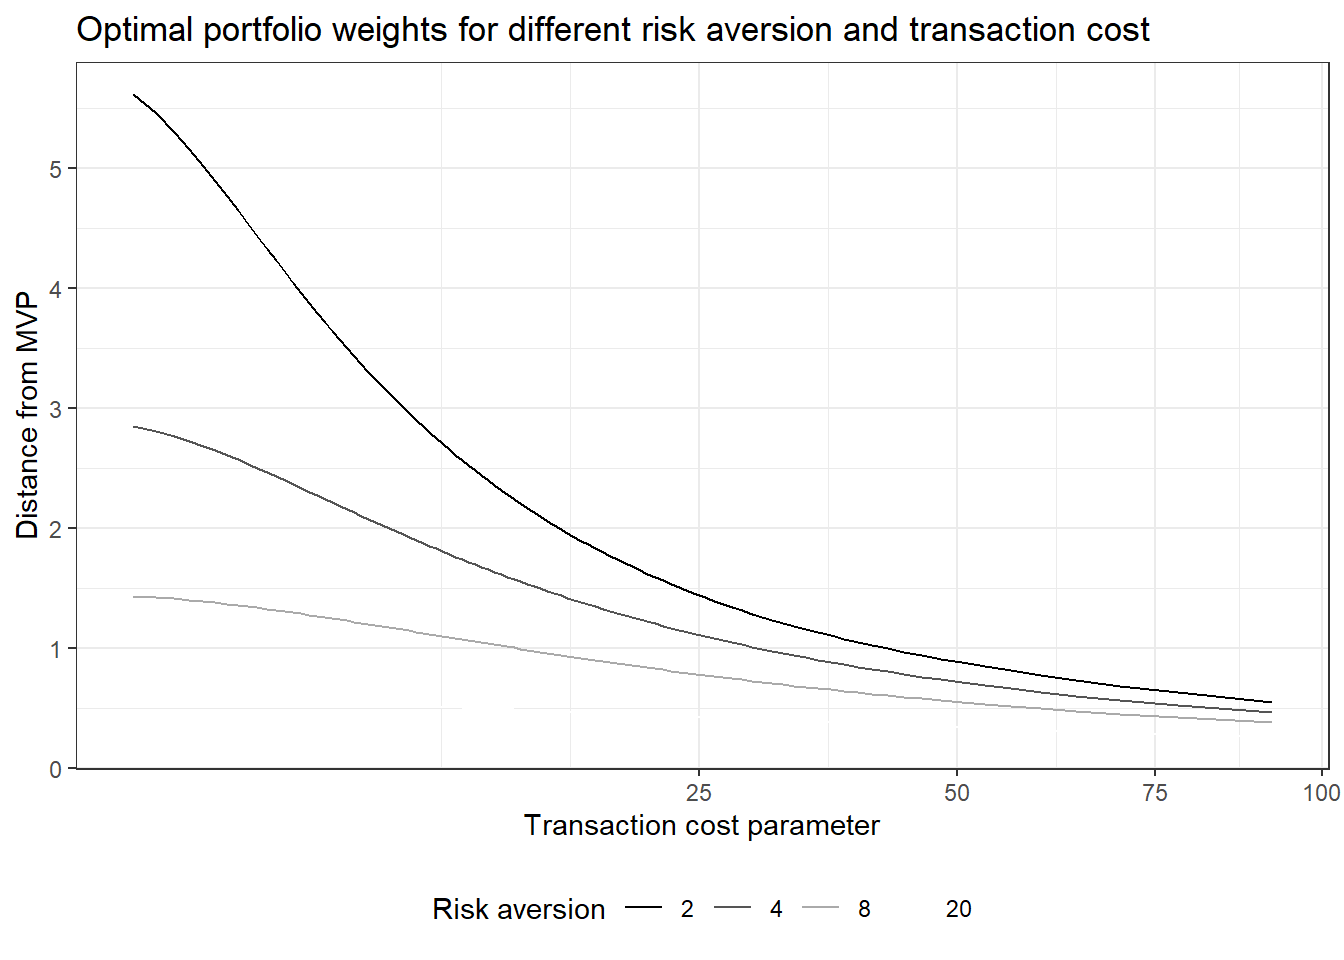
\includegraphics{51_constrained_optimization_and_backtesting_files/figure-latex/unnamed-chunk-5-1} \end{center}

The figure shows that the initial portfolio is always the (sample) MVP and that the higher the transaction costs parameter \(\beta\), the smaller is the rebalancing from the initial portfolio (which we always set to the MVP weights in this example). In addition, if risk aversion \(\gamma\) increases, the efficient portfolio is closer to the MVP weights such that the investor desires less rebalancing from the initial holdings.

\hypertarget{constrained-optimization}{%
\section{Constrained optimization}\label{constrained-optimization}}

Next, we introduce constraints to the above optimization procedure. Very often, typical constraints such as short-selling restrictions prevent analytical solutions for optimal portfolio weights. However, numerical optimization allows computing the solutions to such constrained problems. For the purpose of mean-variance optimization, we rely on the \texttt{solve.QP()} function from the package \texttt{quadprog}.

The function \texttt{solve.QP()} delivers numerical solutions to quadratic programming problems of the form
\[\min(-\mu \omega + 1/2 \omega' \Sigma \omega) \text{ s.t. } A' \omega >= b_0.\]
The function takes one argument (\texttt{meq}) for the number of equality constraints. Therefore, the above matrix \(A\) is simply a vector of ones to ensure that the weights sum up to one. In the case of short-selling constraints, the matrix \(A\) is of the form
\[A = \begin{pmatrix}1 & 1& \ldots&1 \\1 & 0 &\ldots&0\\0 & 1 &\ldots&0\\\vdots&&\ddots&\vdots\\0&0&\ldots&1\end{pmatrix}'\qquad b_0 = \begin{pmatrix}1\\0\\\vdots\\0\end{pmatrix}.\]
Before we dive into unconstrained optimization, we revisit the \emph{unconstrained} problem and replicate the analytical solutions for the minimum variance and efficient portfolio weights from above. We verify that the output is equal to the above solution. Note that we round to the first six digits to avoid differences at higher digits that might arise due to inherent imprecision of numerical estimation procedures. As just discussed, we set \texttt{Amat} to a matrix with a column of ones and \texttt{bvec} to 1 to enforce the constraint that weights must sum up to one. \texttt{meq=1} means that one (out of one) constraints must be satisfied with equality.

\begin{Shaded}
\begin{Highlighting}[]
\NormalTok{n\_industries }\OtherTok{\textless{}{-}} \FunctionTok{ncol}\NormalTok{(industry\_returns)}

\NormalTok{w\_mvp\_numerical }\OtherTok{\textless{}{-}} \FunctionTok{solve.QP}\NormalTok{(}
  \AttributeTok{Dmat =}\NormalTok{ Sigma,}
  \AttributeTok{dvec =} \FunctionTok{rep}\NormalTok{(}\DecValTok{0}\NormalTok{, n\_industries),}
  \AttributeTok{Amat =} \FunctionTok{cbind}\NormalTok{(}\FunctionTok{rep}\NormalTok{(}\DecValTok{1}\NormalTok{, n\_industries)),}
  \AttributeTok{bvec =} \DecValTok{1}\NormalTok{,}
  \AttributeTok{meq =} \DecValTok{1}
\NormalTok{)}

\FunctionTok{all}\NormalTok{(}\FunctionTok{round}\NormalTok{(w\_mvp, }\DecValTok{6}\NormalTok{) }\SpecialCharTok{==} \FunctionTok{round}\NormalTok{(w\_mvp\_numerical}\SpecialCharTok{$}\NormalTok{solution, }\DecValTok{6}\NormalTok{))}
\end{Highlighting}
\end{Shaded}

\begin{verbatim}
## [1] TRUE
\end{verbatim}

\begin{Shaded}
\begin{Highlighting}[]
\NormalTok{w\_efficient\_numerical }\OtherTok{\textless{}{-}} \FunctionTok{solve.QP}\NormalTok{(}
  \AttributeTok{Dmat =} \DecValTok{2} \SpecialCharTok{*}\NormalTok{ Sigma,}
  \AttributeTok{dvec =}\NormalTok{ mu,}
  \AttributeTok{Amat =} \FunctionTok{cbind}\NormalTok{(}\FunctionTok{rep}\NormalTok{(}\DecValTok{1}\NormalTok{, n\_industries)),}
  \AttributeTok{bvec =} \DecValTok{1}\NormalTok{,}
  \AttributeTok{meq =} \DecValTok{1}
\NormalTok{)}

\FunctionTok{all}\NormalTok{(}\FunctionTok{round}\NormalTok{(}\FunctionTok{compute\_efficient\_weight}\NormalTok{(Sigma, mu), }\DecValTok{6}\NormalTok{) }\SpecialCharTok{==} \FunctionTok{round}\NormalTok{(w\_efficient\_numerical}\SpecialCharTok{$}\NormalTok{solution, }\DecValTok{6}\NormalTok{))}
\end{Highlighting}
\end{Shaded}

\begin{verbatim}
## [1] TRUE
\end{verbatim}

For more complex optimization routines, \href{https://cran.r-project.org/web/views/Optimization.html}{this optimization task view} provides an overview of the wast optimization landscape in R.

Next, we approach problems where no analytical solutions exist. First, we additionally impose short-sale constraints, which implies \(N\) inequality constraints if the form \(w_i >=0\).

\begin{Shaded}
\begin{Highlighting}[]
\NormalTok{w\_no\_short\_sale }\OtherTok{\textless{}{-}} \FunctionTok{solve.QP}\NormalTok{(}
  \AttributeTok{Dmat =} \DecValTok{2} \SpecialCharTok{*}\NormalTok{ Sigma,}
  \AttributeTok{dvec =}\NormalTok{ mu,}
  \AttributeTok{Amat =} \FunctionTok{cbind}\NormalTok{(}\DecValTok{1}\NormalTok{, }\FunctionTok{diag}\NormalTok{(n\_industries)),}
  \AttributeTok{bvec =} \FunctionTok{c}\NormalTok{(}\DecValTok{1}\NormalTok{, }\FunctionTok{rep}\NormalTok{(}\DecValTok{0}\NormalTok{, n\_industries)),}
  \AttributeTok{meq =} \DecValTok{1}
\NormalTok{)}
\NormalTok{w\_no\_short\_sale}\SpecialCharTok{$}\NormalTok{solution}
\end{Highlighting}
\end{Shaded}

\begin{verbatim}
##  [1]  6.34e-01 -1.91e-17  1.20e-16 -3.47e-18  6.78e-18
##  [6] -6.24e-17  1.02e-01  2.64e-01  3.38e-22 -2.22e-16
\end{verbatim}

\texttt{solve.QP} is fast because it benefits from a very clear structure with a quadratic objective and linear constraints. However, optimization typically requires more flexibility. As an example, we show how to compute optimal weights, subject to the so-called \href{https://en.wikipedia.org/wiki/Regulation_T}{regulation T-constraint}, which requires that the sum of all absolute portfolio weights is smaller than 1.5. The constraint implies an initial margin requirement of 50\% and, therefore, also a non-linear objective function. Thus, we can no longer rely on \texttt{solve.QP()}. Instead, we rely on the package \texttt{alabama}, which requires a separate definition of objective and constraint functions.

\begin{Shaded}
\begin{Highlighting}[]
\NormalTok{initial\_weights }\OtherTok{\textless{}{-}} \DecValTok{1} \SpecialCharTok{/}\NormalTok{ n\_industries }\SpecialCharTok{*} \FunctionTok{rep}\NormalTok{(}\DecValTok{1}\NormalTok{, n\_industries)}
\NormalTok{objective }\OtherTok{\textless{}{-}} \ControlFlowTok{function}\NormalTok{(w, }\AttributeTok{gamma =} \DecValTok{2}\NormalTok{) }\SpecialCharTok{{-}}\FunctionTok{t}\NormalTok{(w) }\SpecialCharTok{\%*\%}\NormalTok{ (}\DecValTok{1} \SpecialCharTok{+}\NormalTok{ mu) }\SpecialCharTok{+}\NormalTok{ gamma }\SpecialCharTok{/} \DecValTok{2} \SpecialCharTok{*} \FunctionTok{t}\NormalTok{(w) }\SpecialCharTok{\%*\%}\NormalTok{ Sigma }\SpecialCharTok{\%*\%}\NormalTok{ w}
\NormalTok{inequality\_constraints }\OtherTok{\textless{}{-}} \ControlFlowTok{function}\NormalTok{(w, }\AttributeTok{reg\_t =} \FloatTok{1.5}\NormalTok{) \{}
  \FunctionTok{return}\NormalTok{(reg\_t }\SpecialCharTok{{-}} \FunctionTok{sum}\NormalTok{(}\FunctionTok{abs}\NormalTok{(w)))}
\NormalTok{\}}
\NormalTok{equality\_constraints }\OtherTok{\textless{}{-}} \ControlFlowTok{function}\NormalTok{(w) \{}
  \FunctionTok{return}\NormalTok{(}\FunctionTok{sum}\NormalTok{(w) }\SpecialCharTok{{-}} \DecValTok{1}\NormalTok{)}
\NormalTok{\}}

\NormalTok{w\_reg\_t }\OtherTok{\textless{}{-}} \FunctionTok{constrOptim.nl}\NormalTok{(}
  \AttributeTok{par =}\NormalTok{ initial\_weights,}
  \AttributeTok{hin =}\NormalTok{ inequality\_constraints,}
  \AttributeTok{fn =}\NormalTok{ objective,}
  \AttributeTok{heq =}\NormalTok{ equality\_constraints,}
  \AttributeTok{control.outer =} \FunctionTok{list}\NormalTok{(}\AttributeTok{trace =} \ConstantTok{FALSE}\NormalTok{)}
\NormalTok{)}
\NormalTok{w\_reg\_t}\SpecialCharTok{$}\NormalTok{par}
\end{Highlighting}
\end{Shaded}

\begin{verbatim}
##  [1]  4.11e-01 -2.07e-02 -9.00e-02  3.37e-02  8.03e-02
##  [6] -2.25e-08  3.08e-01  3.52e-01  6.25e-02 -1.37e-01
\end{verbatim}

The figure below shows the optimal allocation weights across all 10 industries for the four different strategies considered so far: minimum variance, efficient portfolio with \(\gamma\) = 2, efficient portfolio with short-sale constraints, and the Regulation-T constrained portfolio.

\begin{Shaded}
\begin{Highlighting}[]
\FunctionTok{tibble}\NormalTok{(}
  \StringTok{\textasciigrave{}}\AttributeTok{No short{-}sale}\StringTok{\textasciigrave{}} \OtherTok{=}\NormalTok{ w\_no\_short\_sale}\SpecialCharTok{$}\NormalTok{solution,}
  \StringTok{\textasciigrave{}}\AttributeTok{Minimum Variance}\StringTok{\textasciigrave{}} \OtherTok{=}\NormalTok{ w\_mvp,}
  \StringTok{\textasciigrave{}}\AttributeTok{Efficient portfolio}\StringTok{\textasciigrave{}} \OtherTok{=} \FunctionTok{compute\_efficient\_weight}\NormalTok{(Sigma, mu),}
  \StringTok{\textasciigrave{}}\AttributeTok{Regulation{-}T}\StringTok{\textasciigrave{}} \OtherTok{=}\NormalTok{ w\_reg\_t}\SpecialCharTok{$}\NormalTok{par,}
  \AttributeTok{Industry =} \FunctionTok{colnames}\NormalTok{(industry\_returns)}
\NormalTok{) }\SpecialCharTok{|}\ErrorTok{\textgreater{}}
  \FunctionTok{pivot\_longer}\NormalTok{(}\SpecialCharTok{{-}}\NormalTok{Industry,}
    \AttributeTok{names\_to =} \StringTok{"Strategy"}
\NormalTok{  ) }\SpecialCharTok{|}\ErrorTok{\textgreater{}}
  \FunctionTok{ggplot}\NormalTok{(}\FunctionTok{aes}\NormalTok{(}
    \AttributeTok{fill =}\NormalTok{ Strategy,}
    \AttributeTok{y =}\NormalTok{ value,}
    \AttributeTok{x =}\NormalTok{ Industry}
\NormalTok{  )) }\SpecialCharTok{+}
  \FunctionTok{geom\_bar}\NormalTok{(}\AttributeTok{position =} \StringTok{"dodge"}\NormalTok{, }\AttributeTok{stat =} \StringTok{"identity"}\NormalTok{) }\SpecialCharTok{+}
  \FunctionTok{coord\_flip}\NormalTok{() }\SpecialCharTok{+}
  \FunctionTok{labs}\NormalTok{(}
    \AttributeTok{y =} \StringTok{"Allocation weight"}\NormalTok{,}
    \AttributeTok{title =} \StringTok{" Optimal allocations for different investment rules"}
\NormalTok{  ) }\SpecialCharTok{+}
  \FunctionTok{scale\_y\_continuous}\NormalTok{(}\AttributeTok{labels =}\NormalTok{ scales}\SpecialCharTok{::}\NormalTok{percent)}
\end{Highlighting}
\end{Shaded}

\begin{center}\includegraphics{51_constrained_optimization_and_backtesting_files/figure-latex/unnamed-chunk-9-1} \end{center}

Before we move on, we want to propose a final allocation strategy, which reflects a somewhat more realistic structure of transaction costs instead of the quadratic specification used above. The function below computes efficient portfolio weights while adjusting for \(L_1\) transaction costs \(\beta\sum\limits_{i=1}^N |(w_{i, t+1} - w_{i, t^+})|\). No closed-form solution exists, and we rely on non-linear optimization procedures.

\begin{Shaded}
\begin{Highlighting}[]
\NormalTok{compute\_efficient\_weight\_L1\_TC }\OtherTok{\textless{}{-}} \ControlFlowTok{function}\NormalTok{(mu,}
\NormalTok{                                           Sigma,}
                                           \AttributeTok{gamma =} \DecValTok{2}\NormalTok{,}
                                           \AttributeTok{beta =} \DecValTok{0}\NormalTok{,}
                                           \AttributeTok{initial\_weights =} \DecValTok{1} \SpecialCharTok{/} \FunctionTok{ncol}\NormalTok{(sigma) }\SpecialCharTok{*} \FunctionTok{rep}\NormalTok{(}\DecValTok{1}\NormalTok{, }\FunctionTok{ncol}\NormalTok{(sigma))) \{}
\NormalTok{  objective }\OtherTok{\textless{}{-}} \ControlFlowTok{function}\NormalTok{(w) }\SpecialCharTok{{-}}\FunctionTok{t}\NormalTok{(w) }\SpecialCharTok{\%*\%}\NormalTok{ mu }\SpecialCharTok{+}\NormalTok{ gamma }\SpecialCharTok{/} \DecValTok{2} \SpecialCharTok{*} \FunctionTok{t}\NormalTok{(w) }\SpecialCharTok{\%*\%}\NormalTok{ Sigma }\SpecialCharTok{\%*\%}\NormalTok{ w }\SpecialCharTok{+}\NormalTok{ (beta }\SpecialCharTok{/} \DecValTok{10000}\NormalTok{) }\SpecialCharTok{/} \DecValTok{2} \SpecialCharTok{*} \FunctionTok{sum}\NormalTok{(}\FunctionTok{abs}\NormalTok{(w }\SpecialCharTok{{-}}\NormalTok{ initial\_weights))}

\NormalTok{  w\_optimal }\OtherTok{\textless{}{-}} \FunctionTok{constrOptim.nl}\NormalTok{(}
    \AttributeTok{par =}\NormalTok{ initial\_weights,}
    \AttributeTok{fn =}\NormalTok{ objective,}
    \AttributeTok{heq =} \ControlFlowTok{function}\NormalTok{(w) \{}
      \FunctionTok{sum}\NormalTok{(w) }\SpecialCharTok{{-}} \DecValTok{1}
\NormalTok{    \},}
    \AttributeTok{control.outer =} \FunctionTok{list}\NormalTok{(}\AttributeTok{trace =} \ConstantTok{FALSE}\NormalTok{)}
\NormalTok{  )}

\NormalTok{  w\_optimal}\SpecialCharTok{$}\NormalTok{par}
\NormalTok{\}}
\end{Highlighting}
\end{Shaded}

\hypertarget{out-of-sample-backtesting}{%
\section{Out-of-sample backtesting}\label{out-of-sample-backtesting}}

For the sake of simplicity, we committed one fundamental error in computing portfolio weights above. We used the full sample of the data to determine the optimal allocation. To implement this strategy at the beginning of the 2000s, you will need to know how the returns will evolve until 2020. While interesting from a methodological point of view, we cannot evaluate the performance of the portfolios in a reasonable out-of-sample fashion. We do so next in a backtesting application for three strategies. For the backtest, we recompute optimal weights just based on past available data.

\begin{Shaded}
\begin{Highlighting}[]
\NormalTok{window\_length }\OtherTok{\textless{}{-}} \DecValTok{120}
\NormalTok{periods }\OtherTok{\textless{}{-}} \FunctionTok{nrow}\NormalTok{(industry\_returns) }\SpecialCharTok{{-}}\NormalTok{ window\_length}

\NormalTok{beta }\OtherTok{\textless{}{-}} \DecValTok{50}
\NormalTok{gamma }\OtherTok{\textless{}{-}} \DecValTok{2}

\NormalTok{performance\_values }\OtherTok{\textless{}{-}} \FunctionTok{matrix}\NormalTok{(}\ConstantTok{NA}\NormalTok{,}
  \AttributeTok{nrow =}\NormalTok{ periods,}
  \AttributeTok{ncol =} \DecValTok{3}
\NormalTok{) }\CommentTok{\# A matrix to collect all returns}
\FunctionTok{colnames}\NormalTok{(performance\_values) }\OtherTok{\textless{}{-}} \FunctionTok{c}\NormalTok{(}\StringTok{"raw\_return"}\NormalTok{, }\StringTok{"turnover"}\NormalTok{, }\StringTok{"net\_return"}\NormalTok{)}

\NormalTok{performance\_values }\OtherTok{\textless{}{-}} \FunctionTok{list}\NormalTok{(}
  \StringTok{"MV (TC)"} \OtherTok{=}\NormalTok{ performance\_values,}
  \StringTok{"Naive"} \OtherTok{=}\NormalTok{ performance\_values,}
  \StringTok{"MV"} \OtherTok{=}\NormalTok{ performance\_values}
\NormalTok{)}

\NormalTok{w\_prev\_1 }\OtherTok{\textless{}{-}}\NormalTok{ w\_prev\_2 }\OtherTok{\textless{}{-}}\NormalTok{ w\_prev\_3 }\OtherTok{\textless{}{-}} \FunctionTok{rep}\NormalTok{(}
  \DecValTok{1} \SpecialCharTok{/}\NormalTok{ n\_industries,}
\NormalTok{  n\_industries}
\NormalTok{)}
\end{Highlighting}
\end{Shaded}

We also define two helper functions: one to adjust the weights due to returns and one for performance evaluation, where we compute realized returns net of transaction costs.

\begin{Shaded}
\begin{Highlighting}[]
\NormalTok{adjust\_weights }\OtherTok{\textless{}{-}} \ControlFlowTok{function}\NormalTok{(w, next\_return) \{}
\NormalTok{  w\_prev }\OtherTok{\textless{}{-}} \DecValTok{1} \SpecialCharTok{+}\NormalTok{ w }\SpecialCharTok{*}\NormalTok{ next\_return}
  \FunctionTok{as.numeric}\NormalTok{(w\_prev }\SpecialCharTok{/} \FunctionTok{sum}\NormalTok{(}\FunctionTok{as.vector}\NormalTok{(w\_prev)))}
\NormalTok{\}}

\NormalTok{evaluate\_performance }\OtherTok{\textless{}{-}} \ControlFlowTok{function}\NormalTok{(w, w\_previous, next\_return, }\AttributeTok{beta =} \DecValTok{50}\NormalTok{) \{}
\NormalTok{  raw\_return }\OtherTok{\textless{}{-}} \FunctionTok{as.matrix}\NormalTok{(next\_return) }\SpecialCharTok{\%*\%}\NormalTok{ w}
\NormalTok{  turnover }\OtherTok{\textless{}{-}} \FunctionTok{sum}\NormalTok{(}\FunctionTok{abs}\NormalTok{(w }\SpecialCharTok{{-}}\NormalTok{ w\_previous))}
\NormalTok{  net\_return }\OtherTok{\textless{}{-}}\NormalTok{ raw\_return }\SpecialCharTok{{-}}\NormalTok{ beta }\SpecialCharTok{/} \DecValTok{10000} \SpecialCharTok{*}\NormalTok{ turnover}
  \FunctionTok{c}\NormalTok{(raw\_return, turnover, net\_return)}
\NormalTok{\}}
\end{Highlighting}
\end{Shaded}

The lines above define the general setup. We consider 120 periods from the past to update the parameter estimates before recomputing portfolio weights. Then, we update portfolio weights which is costly and affects the performance. The portfolio weights determine the portfolio return. A period later, the current portfolio weights have changed and form the foundation for transaction costs incurred in the next period. We consider three different competing strategies: the mean-variance efficient portfolio, the mean-variance efficient portfolio with ex-ante adjustment for transaction costs, and the naive portfolio, which allocates wealth equally across the different assets.

The following code chunk performs rolling-window estimation. In each period, the estimation window contains the returns available up to the current period. Note that we use the sample moments, but you might use more advanced estimators in practice.

\begin{Shaded}
\begin{Highlighting}[]
\ControlFlowTok{for}\NormalTok{ (p }\ControlFlowTok{in} \DecValTok{1}\SpecialCharTok{:}\NormalTok{periods) \{}
\NormalTok{  returns\_window }\OtherTok{\textless{}{-}}\NormalTok{ industry\_returns[p}\SpecialCharTok{:}\NormalTok{(p }\SpecialCharTok{+}\NormalTok{ window\_length }\SpecialCharTok{{-}} \DecValTok{1}\NormalTok{), ]}
\NormalTok{  next\_return }\OtherTok{\textless{}{-}}\NormalTok{ industry\_returns[p }\SpecialCharTok{+}\NormalTok{ window\_length, ] }\SpecialCharTok{|}\ErrorTok{\textgreater{}} \FunctionTok{as.matrix}\NormalTok{()}

\NormalTok{  Sigma }\OtherTok{\textless{}{-}} \FunctionTok{cov}\NormalTok{(returns\_window)}
\NormalTok{  mu }\OtherTok{\textless{}{-}} \DecValTok{0} \SpecialCharTok{*} \FunctionTok{colMeans}\NormalTok{(returns\_window)}

  \CommentTok{\# Transaction{-}cost adjusted portfolio}
\NormalTok{  w\_1 }\OtherTok{\textless{}{-}} \FunctionTok{compute\_efficient\_weight\_L1\_TC}\NormalTok{(}
    \AttributeTok{mu =}\NormalTok{ mu,}
    \AttributeTok{Sigma =}\NormalTok{ Sigma,}
    \AttributeTok{beta =}\NormalTok{ beta,}
    \AttributeTok{gamma =}\NormalTok{ gamma,}
    \AttributeTok{initial\_weights =}\NormalTok{ w\_prev\_1}
\NormalTok{  )}

\NormalTok{  performance\_values[[}\DecValTok{1}\NormalTok{]][p, ] }\OtherTok{\textless{}{-}} \FunctionTok{evaluate\_performance}\NormalTok{(w\_1,}
\NormalTok{    w\_prev\_1,}
\NormalTok{    next\_return,}
    \AttributeTok{beta =}\NormalTok{ beta}
\NormalTok{  )}

\NormalTok{  w\_prev\_1 }\OtherTok{\textless{}{-}} \FunctionTok{adjust\_weights}\NormalTok{(w\_1, next\_return)}

  \CommentTok{\# Naive portfolio}
\NormalTok{  w\_2 }\OtherTok{\textless{}{-}} \FunctionTok{rep}\NormalTok{(}\DecValTok{1} \SpecialCharTok{/}\NormalTok{ n\_industries, n\_industries)}

\NormalTok{  performance\_values[[}\DecValTok{2}\NormalTok{]][p, ] }\OtherTok{\textless{}{-}} \FunctionTok{evaluate\_performance}\NormalTok{(}
\NormalTok{    w\_2,}
\NormalTok{    w\_prev\_2,}
\NormalTok{    next\_return}
\NormalTok{  )}

\NormalTok{  w\_prev\_2 }\OtherTok{\textless{}{-}} \FunctionTok{adjust\_weights}\NormalTok{(w\_2, next\_return)}

  \CommentTok{\# Mean{-}variance efficient portfolio (w/o transaction costs)}
\NormalTok{  w\_3 }\OtherTok{\textless{}{-}} \FunctionTok{compute\_efficient\_weight}\NormalTok{(}
    \AttributeTok{Sigma =}\NormalTok{ Sigma,}
    \AttributeTok{mu =}\NormalTok{ mu,}
    \AttributeTok{gamma =}\NormalTok{ gamma}
\NormalTok{  )}

\NormalTok{  performance\_values[[}\DecValTok{3}\NormalTok{]][p, ] }\OtherTok{\textless{}{-}} \FunctionTok{evaluate\_performance}\NormalTok{(}
\NormalTok{    w\_3,}
\NormalTok{    w\_prev\_3,}
\NormalTok{    next\_return}
\NormalTok{  )}

\NormalTok{  w\_prev\_3 }\OtherTok{\textless{}{-}} \FunctionTok{adjust\_weights}\NormalTok{(w\_3, next\_return)}
\NormalTok{\}}
\end{Highlighting}
\end{Shaded}

Finally, we get to the evaluation of the portfolio strategies \emph{net-of-transaction costs}. Note that we compute annualized returns and standard deviations.

\begin{Shaded}
\begin{Highlighting}[]
\NormalTok{performance }\OtherTok{\textless{}{-}} \FunctionTok{lapply}\NormalTok{(performance\_values, as\_tibble) }\SpecialCharTok{|}\ErrorTok{\textgreater{}}
  \FunctionTok{bind\_rows}\NormalTok{(}\AttributeTok{.id =} \StringTok{"strategy"}\NormalTok{)}

\NormalTok{performance }\SpecialCharTok{|}\ErrorTok{\textgreater{}}
  \FunctionTok{group\_by}\NormalTok{(strategy) }\SpecialCharTok{|}\ErrorTok{\textgreater{}}
  \FunctionTok{summarize}\NormalTok{(}
    \AttributeTok{Mean =} \DecValTok{12} \SpecialCharTok{*} \FunctionTok{mean}\NormalTok{(}\DecValTok{100} \SpecialCharTok{*}\NormalTok{ net\_return),}
    \AttributeTok{SD =} \FunctionTok{sqrt}\NormalTok{(}\DecValTok{12}\NormalTok{) }\SpecialCharTok{*} \FunctionTok{sd}\NormalTok{(}\DecValTok{100} \SpecialCharTok{*}\NormalTok{ net\_return),}
    \StringTok{\textasciigrave{}}\AttributeTok{Sharpe ratio}\StringTok{\textasciigrave{}} \OtherTok{=} \FunctionTok{if\_else}\NormalTok{(Mean }\SpecialCharTok{\textgreater{}} \DecValTok{0}\NormalTok{,}
\NormalTok{      Mean }\SpecialCharTok{/}\NormalTok{ SD,}
      \ConstantTok{NA\_real\_}
\NormalTok{    ),}
    \AttributeTok{Turnover =} \DecValTok{100} \SpecialCharTok{*} \FunctionTok{mean}\NormalTok{(turnover)}
\NormalTok{  )}
\end{Highlighting}
\end{Shaded}

\begin{verbatim}
## # A tibble: 3 x 5
##   strategy   Mean    SD `Sharpe ratio` Turnover
##   <chr>     <dbl> <dbl>          <dbl>    <dbl>
## 1 MV       -0.637  12.4         NA     214.    
## 2 MV (TC)  12.1    15.1          0.802   0.0311
## 3 Naive    12.1    15.1          0.801   0.229
\end{verbatim}

The results clearly speak against mean-variance optimization. Turnover is huge when the investor only considers her portfolio's expected return and variance. Effectively, the mean-variance portfolio generates a \emph{negative} annualized return after adjusting for transaction costs. At the same time, the naive portfolio turns out to perform very well. In fact, the performance gains of the transaction-cost adjusted mean-variance portfolio are small. The out-of-sample Sharpe ratio is slightly higher than for the naive portfolio. Note the extreme effect of turnover penalization on turnover: \emph{MV (TC)} effectively resembles a buy-and-hold strategy which only updates the portfolio once the estimated parameters \(\hat\mu_t\) and \(\hat\Sigma_t\)indicate that the current allocation is too far away from the optimal theoretical portfolio.

\hypertarget{exercises-11}{%
\section{Exercises}\label{exercises-11}}

\begin{enumerate}
\def\labelenumi{\arabic{enumi}.}
\tightlist
\item
  We argue that an investor with a quadratic utility function with certainty equivalent \[\max_w CE(w) = \omega'\mu - \frac{\gamma}{2} \omega'\Sigma \omega \text{ s.t. } \iota'\omega = 1\]
  faces an equivalent optimization problem to a framework where portfolio weights are chosen with the aim to minimize volatility given a pre-specified level or expected returns
  \[\min_w \omega'\Sigma \omega \text{ s.t. } \omega'\mu = \bar\mu \text{ and } \iota'\omega = 1. \] Proof that there is an equivalence between the optimal portfolio weights in both cases.
\item
  Consider the portfolio choice problem for transaction-cost adjusted certainty equivalent maximization with risk aversion parameter \(\gamma\)
  \[\omega_{t+1} ^* :=  \arg\max_{\omega \in \mathbb{R}^N,  \iota'\omega = 1} \omega'\mu - \nu_t (\omega, \beta) - \frac{\gamma}{2}\omega'\Sigma\omega\]
  where \(\Sigma\) and \(\mu\) are (estimators of) the variance-covariance matrix of the returns and the vector of expected returns. Assume for now that transaction costs are quadratic in rebalancing \textbf{and} proportional to stock illiquidity such that
  \[\nu_t\left(\omega, \mathbf{\beta}\right) := \frac{\beta}{2} \left(\omega - \omega_{t^+}\right)'B\left(\omega - \omega_{t^+}\right)\] where \(B = \text{diag}(ill_1, \ldots, ill_N)\) is a diagonal matrix where \(ill_1, \ldots, ill_N\). Derive a closed-form solution for the mean-variance efficient portfolio \(\omega_{t+1} ^*\) based on the transaction cost specification above. Discuss the effect of illiquidity \(ill_i\) on the individual portfolio weights relative to an investor that myopically ignores transaction costs in her decision.
\item
  Use the solution from the previous exercise to update the function \texttt{compute\_efficient\_weight} such that you can compute optimal weights conditional on a matrix \(B\) with illiquidity measures.
\item
  Illustrate the evolution of the \emph{optimal} weights from the naive portfolio to the efficient portfolio in the mean-standard deviation diagram.
\item
  Is it always optimal to choose the same \(\beta\) in the optimization problem than the value used in evaluating the portfolio performance? In other words: Can it be optimal to choose theoretically sub-optimal portfolios based on transaction cost considerations that do not reflect the actual incurred costs? Evaluate the out-of-sample Sharpe ratio after transaction costs for a range of different values of imposed \(\beta\) values.
\end{enumerate}

\hypertarget{refs}{}
\begin{CSLReferences}{0}{0}
\end{CSLReferences}

\hypertarget{appendix-appendix}{%
\appendix \addcontentsline{toc}{chapter}{\appendixname}}


\hypertarget{cover-design}{%
\chapter{Cover design}\label{cover-design}}

\begin{Shaded}
\begin{Highlighting}[]
\FunctionTok{library}\NormalTok{(tidyverse)}
\FunctionTok{library}\NormalTok{(RSQLite)}
\FunctionTok{library}\NormalTok{(wesanderson)}

\NormalTok{tidy\_finance }\OtherTok{\textless{}{-}} \FunctionTok{dbConnect}\NormalTok{(}\FunctionTok{SQLite}\NormalTok{(), }\StringTok{"data/tidy\_finance.sqlite"}\NormalTok{, }\AttributeTok{extended\_types =} \ConstantTok{TRUE}\NormalTok{)}
\NormalTok{mfac }\OtherTok{\textless{}{-}} \FunctionTok{tbl}\NormalTok{(tidy\_finance, }\StringTok{"factors\_ff\_daily"}\NormalTok{) }\SpecialCharTok{\%\textgreater{}\%}
  \FunctionTok{collect}\NormalTok{()}

\NormalTok{cp }\OtherTok{\textless{}{-}} \FunctionTok{coord\_polar}\NormalTok{(}\AttributeTok{direction =} \SpecialCharTok{{-}}\DecValTok{1}\NormalTok{, }\AttributeTok{clip =} \StringTok{"on"}\NormalTok{)}
\NormalTok{cp}\SpecialCharTok{$}\NormalTok{is\_free }\OtherTok{\textless{}{-}} \ControlFlowTok{function}\NormalTok{() }\ConstantTok{TRUE}

\NormalTok{plot\_data }\OtherTok{\textless{}{-}}\NormalTok{ mfac }\SpecialCharTok{\%\textgreater{}\%}
  \FunctionTok{select}\NormalTok{(date, mkt\_excess) }\SpecialCharTok{\%\textgreater{}\%}
  \FunctionTok{group\_by}\NormalTok{(}\AttributeTok{year =}\NormalTok{ lubridate}\SpecialCharTok{::}\FunctionTok{floor\_date}\NormalTok{(date, }\StringTok{"year"}\NormalTok{)) }\SpecialCharTok{\%\textgreater{}\%}
  \FunctionTok{mutate}\NormalTok{(}\AttributeTok{group\_id =} \FunctionTok{cur\_group\_id}\NormalTok{())}

\NormalTok{plot\_data }\OtherTok{\textless{}{-}}\NormalTok{ plot\_data }\SpecialCharTok{\%\textgreater{}\%}
  \FunctionTok{mutate}\NormalTok{(}
    \AttributeTok{group\_id =} \FunctionTok{if\_else}\NormalTok{(group\_id }\SpecialCharTok{\textgreater{}=} \DecValTok{28}\NormalTok{, group\_id }\SpecialCharTok{+} \DecValTok{4}\NormalTok{, group\_id }\SpecialCharTok{+} \DecValTok{0}\NormalTok{),}
    \AttributeTok{group\_id =} \FunctionTok{if\_else}\NormalTok{(group\_id }\SpecialCharTok{\textgreater{}=} \DecValTok{36}\NormalTok{, group\_id }\SpecialCharTok{+} \DecValTok{4}\NormalTok{, group\_id }\SpecialCharTok{+} \DecValTok{0}\NormalTok{),}
    \AttributeTok{group\_id =} \FunctionTok{if\_else}\NormalTok{(group\_id }\SpecialCharTok{\textgreater{}=} \DecValTok{44}\NormalTok{, group\_id }\SpecialCharTok{+} \DecValTok{4}\NormalTok{, group\_id }\SpecialCharTok{+} \DecValTok{0}\NormalTok{)}
\NormalTok{  ) }\SpecialCharTok{\%\textgreater{}\%}
  \FunctionTok{bind\_rows}\NormalTok{(plot\_data }\SpecialCharTok{\%\textgreater{}\%}
    \FunctionTok{filter}\NormalTok{(group\_id }\SpecialCharTok{\%in\%} \FunctionTok{c}\NormalTok{(}\DecValTok{28}\SpecialCharTok{:}\DecValTok{31}\NormalTok{, }\DecValTok{36}\SpecialCharTok{:}\DecValTok{39}\NormalTok{, }\DecValTok{44}\SpecialCharTok{:}\DecValTok{47}\NormalTok{)) }\SpecialCharTok{\%\textgreater{}\%}
    \FunctionTok{mutate}\NormalTok{(}\AttributeTok{mkt\_excess =} \ConstantTok{NA}\NormalTok{)) }\SpecialCharTok{\%\textgreater{}\%}
  \FunctionTok{group\_by}\NormalTok{(group\_id) }\SpecialCharTok{\%\textgreater{}\%}
  \FunctionTok{mutate}\NormalTok{(}
    \AttributeTok{day =} \DecValTok{2} \SpecialCharTok{*}\NormalTok{ pi }\SpecialCharTok{*}\NormalTok{ (}\DecValTok{1}\SpecialCharTok{:}\FunctionTok{n}\NormalTok{()) }\SpecialCharTok{/} \DecValTok{252}\NormalTok{,}
    \AttributeTok{ymin =} \FunctionTok{pmin}\NormalTok{(}\DecValTok{1} \SpecialCharTok{+}\NormalTok{ mkt\_excess, }\DecValTok{1}\NormalTok{),}
    \AttributeTok{ymax =} \FunctionTok{pmax}\NormalTok{(}\DecValTok{1} \SpecialCharTok{+}\NormalTok{ mkt\_excess, }\DecValTok{1}\NormalTok{),}
    \AttributeTok{vola =} \FunctionTok{sd}\NormalTok{(mkt\_excess)}
\NormalTok{  ) }\SpecialCharTok{\%\textgreater{}\%}
  \FunctionTok{filter}\NormalTok{(year }\SpecialCharTok{\textgreater{}=} \StringTok{"1961{-}01{-}01"}\NormalTok{)}

\NormalTok{colors }\OtherTok{\textless{}{-}} \FunctionTok{wes\_palette}\NormalTok{(}\StringTok{"Zissou1"}\NormalTok{, }\FunctionTok{n\_groups}\NormalTok{(plot\_data), }\AttributeTok{type =} \StringTok{"continuous"}\NormalTok{)}
\NormalTok{levels }\OtherTok{\textless{}{-}}\NormalTok{ plot\_data }\SpecialCharTok{\%\textgreater{}\%}
  \FunctionTok{distinct}\NormalTok{(group\_id, vola) }\SpecialCharTok{\%\textgreater{}\%}
  \FunctionTok{arrange}\NormalTok{(vola) }\SpecialCharTok{\%\textgreater{}\%}
  \FunctionTok{pull}\NormalTok{(vola)}

\NormalTok{plot }\OtherTok{\textless{}{-}}\NormalTok{ plot\_data }\SpecialCharTok{\%\textgreater{}\%}
  \FunctionTok{mutate}\NormalTok{(}\AttributeTok{vola =} \FunctionTok{factor}\NormalTok{(vola, }\AttributeTok{levels =}\NormalTok{ levels)) }\SpecialCharTok{\%\textgreater{}\%}
  \FunctionTok{ggplot}\NormalTok{() }\SpecialCharTok{+}
  \FunctionTok{aes}\NormalTok{(}\AttributeTok{x =}\NormalTok{ day, }\AttributeTok{y =}\NormalTok{ mkt\_excess, }\AttributeTok{group =}\NormalTok{ group\_id, }\AttributeTok{fill =}\NormalTok{ vola) }\SpecialCharTok{+}
\NormalTok{  cp }\SpecialCharTok{+}
  \FunctionTok{geom\_ribbon}\NormalTok{(}\FunctionTok{aes}\NormalTok{(}
    \AttributeTok{ymin =}\NormalTok{ ymin,}
    \AttributeTok{ymax =}\NormalTok{ ymax,}
    \AttributeTok{fill =} \FunctionTok{as\_factor}\NormalTok{(vola)}
\NormalTok{  ), }\AttributeTok{alpha =} \FloatTok{0.90}\NormalTok{) }\SpecialCharTok{+}
  \FunctionTok{theme\_void}\NormalTok{() }\SpecialCharTok{+}
  \FunctionTok{facet\_wrap}\NormalTok{(}\SpecialCharTok{\textasciitilde{}}\NormalTok{group\_id, }\AttributeTok{ncol =} \DecValTok{8}\NormalTok{, }\AttributeTok{scales =} \StringTok{"free"}\NormalTok{) }\SpecialCharTok{+}
  \FunctionTok{theme}\NormalTok{(}
    \AttributeTok{strip.text.x =} \FunctionTok{element\_blank}\NormalTok{(),}
    \AttributeTok{legend.position =} \StringTok{"None"}\NormalTok{,}
    \AttributeTok{panel.spacing =} \FunctionTok{unit}\NormalTok{(}\SpecialCharTok{{-}}\DecValTok{5}\NormalTok{, }\StringTok{"lines"}\NormalTok{)}
\NormalTok{  ) }\SpecialCharTok{+}
  \FunctionTok{scale\_fill\_manual}\NormalTok{(}\AttributeTok{values =}\NormalTok{ colors)}

\CommentTok{\# ggsave(}
\CommentTok{\#   plot = plot, width = 8, height = 9,}
\CommentTok{\#   filename = "cover.jpg", bg = "white"}
\CommentTok{\# )}
\end{Highlighting}
\end{Shaded}


  \bibliography{book.bib}

\printindex

\end{document}
